% Options for packages loaded elsewhere
\PassOptionsToPackage{unicode}{hyperref}
\PassOptionsToPackage{hyphens}{url}
\PassOptionsToPackage{dvipsnames,svgnames,x11names}{xcolor}
\documentclass[
  10pt,
]{ltjsarticle}
\usepackage{xcolor}
\usepackage[margin=2.2cm]{geometry}
\usepackage{amsmath,amssymb}
\setcounter{secnumdepth}{-\maxdimen} % remove section numbering
\usepackage{iftex}
\ifPDFTeX
  \usepackage[T1]{fontenc}
  \usepackage[utf8]{inputenc}
  \usepackage{textcomp} % provide euro and other symbols
\else % if luatex or xetex
  \usepackage{unicode-math} % this also loads fontspec
  \defaultfontfeatures{Scale=MatchLowercase}
  \defaultfontfeatures[\rmfamily]{Ligatures=TeX,Scale=1}
\fi
\usepackage{lmodern}
\ifPDFTeX\else
  % xetex/luatex font selection
\fi
% Use upquote if available, for straight quotes in verbatim environments
\IfFileExists{upquote.sty}{\usepackage{upquote}}{}
\IfFileExists{microtype.sty}{% use microtype if available
  \usepackage[]{microtype}
  \UseMicrotypeSet[protrusion]{basicmath} % disable protrusion for tt fonts
}{}
\makeatletter
\@ifundefined{KOMAClassName}{% if non-KOMA class
  \IfFileExists{parskip.sty}{%
    \usepackage{parskip}
  }{% else
    \setlength{\parindent}{0pt}
    \setlength{\parskip}{6pt plus 2pt minus 1pt}}
}{% if KOMA class
  \KOMAoptions{parskip=half}}
\makeatother
\usepackage{color}
\usepackage{fancyvrb}
\newcommand{\VerbBar}{|}
\newcommand{\VERB}{\Verb[commandchars=\\\{\}]}
\DefineVerbatimEnvironment{Highlighting}{Verbatim}{commandchars=\\\{\}}
% Add ',fontsize=\small' for more characters per line
\newenvironment{Shaded}{}{}
\newcommand{\AlertTok}[1]{\textcolor[rgb]{1.00,0.00,0.00}{\textbf{#1}}}
\newcommand{\AnnotationTok}[1]{\textcolor[rgb]{0.38,0.63,0.69}{\textbf{\textit{#1}}}}
\newcommand{\AttributeTok}[1]{\textcolor[rgb]{0.49,0.56,0.16}{#1}}
\newcommand{\BaseNTok}[1]{\textcolor[rgb]{0.25,0.63,0.44}{#1}}
\newcommand{\BuiltInTok}[1]{\textcolor[rgb]{0.00,0.50,0.00}{#1}}
\newcommand{\CharTok}[1]{\textcolor[rgb]{0.25,0.44,0.63}{#1}}
\newcommand{\CommentTok}[1]{\textcolor[rgb]{0.38,0.63,0.69}{\textit{#1}}}
\newcommand{\CommentVarTok}[1]{\textcolor[rgb]{0.38,0.63,0.69}{\textbf{\textit{#1}}}}
\newcommand{\ConstantTok}[1]{\textcolor[rgb]{0.53,0.00,0.00}{#1}}
\newcommand{\ControlFlowTok}[1]{\textcolor[rgb]{0.00,0.44,0.13}{\textbf{#1}}}
\newcommand{\DataTypeTok}[1]{\textcolor[rgb]{0.56,0.13,0.00}{#1}}
\newcommand{\DecValTok}[1]{\textcolor[rgb]{0.25,0.63,0.44}{#1}}
\newcommand{\DocumentationTok}[1]{\textcolor[rgb]{0.73,0.13,0.13}{\textit{#1}}}
\newcommand{\ErrorTok}[1]{\textcolor[rgb]{1.00,0.00,0.00}{\textbf{#1}}}
\newcommand{\ExtensionTok}[1]{#1}
\newcommand{\FloatTok}[1]{\textcolor[rgb]{0.25,0.63,0.44}{#1}}
\newcommand{\FunctionTok}[1]{\textcolor[rgb]{0.02,0.16,0.49}{#1}}
\newcommand{\ImportTok}[1]{\textcolor[rgb]{0.00,0.50,0.00}{\textbf{#1}}}
\newcommand{\InformationTok}[1]{\textcolor[rgb]{0.38,0.63,0.69}{\textbf{\textit{#1}}}}
\newcommand{\KeywordTok}[1]{\textcolor[rgb]{0.00,0.44,0.13}{\textbf{#1}}}
\newcommand{\NormalTok}[1]{#1}
\newcommand{\OperatorTok}[1]{\textcolor[rgb]{0.40,0.40,0.40}{#1}}
\newcommand{\OtherTok}[1]{\textcolor[rgb]{0.00,0.44,0.13}{#1}}
\newcommand{\PreprocessorTok}[1]{\textcolor[rgb]{0.74,0.48,0.00}{#1}}
\newcommand{\RegionMarkerTok}[1]{#1}
\newcommand{\SpecialCharTok}[1]{\textcolor[rgb]{0.25,0.44,0.63}{#1}}
\newcommand{\SpecialStringTok}[1]{\textcolor[rgb]{0.73,0.40,0.53}{#1}}
\newcommand{\StringTok}[1]{\textcolor[rgb]{0.25,0.44,0.63}{#1}}
\newcommand{\VariableTok}[1]{\textcolor[rgb]{0.10,0.09,0.49}{#1}}
\newcommand{\VerbatimStringTok}[1]{\textcolor[rgb]{0.25,0.44,0.63}{#1}}
\newcommand{\WarningTok}[1]{\textcolor[rgb]{0.38,0.63,0.69}{\textbf{\textit{#1}}}}
\usepackage{longtable,booktabs,array}
\newcounter{none} % for unnumbered tables
\usepackage{calc} % for calculating minipage widths
% Correct order of tables after \paragraph or \subparagraph
\usepackage{etoolbox}
\makeatletter
\patchcmd\longtable{\par}{\if@noskipsec\mbox{}\fi\par}{}{}
\makeatother
% Allow footnotes in longtable head/foot
\IfFileExists{footnotehyper.sty}{\usepackage{footnotehyper}}{\usepackage{footnote}}
\makesavenoteenv{longtable}
\usepackage{graphicx}
\makeatletter
\newsavebox\pandoc@box
\newcommand*\pandocbounded[1]{% scales image to fit in text height/width
  \sbox\pandoc@box{#1}%
  \Gscale@div\@tempa{\textheight}{\dimexpr\ht\pandoc@box+\dp\pandoc@box\relax}%
  \Gscale@div\@tempb{\linewidth}{\wd\pandoc@box}%
  \ifdim\@tempb\p@<\@tempa\p@\let\@tempa\@tempb\fi% select the smaller of both
  \ifdim\@tempa\p@<\p@\scalebox{\@tempa}{\usebox\pandoc@box}%
  \else\usebox{\pandoc@box}%
  \fi%
}
% Set default figure placement to htbp
\def\fps@figure{htbp}
\makeatother
\ifLuaTeX
  \usepackage{luacolor}
  \usepackage[soul]{lua-ul}
\else
  \usepackage{soul}
\fi
\setlength{\emergencystretch}{3em} % prevent overfull lines
\providecommand{\tightlist}{%
  \setlength{\itemsep}{0pt}\setlength{\parskip}{0pt}}
\usepackage{bookmark}
\IfFileExists{xurl.sty}{\usepackage{xurl}}{} % add URL line breaks if available
\urlstyle{same}
\hypersetup{
  colorlinks=true,
  linkcolor={blue},
  filecolor={Maroon},
  citecolor={Blue},
  urlcolor={blue},
  pdfcreator={LaTeX via pandoc}}

\author{}
\date{}

\begin{document}

{
\setcounter{tocdepth}{3}
\tableofcontents
}
\section{ゼロ閉塞は4次元だった --- 主張案
v4}\label{ux30bcux30edux9589ux585eux306f4ux6b21ux5143ux3060ux3063ux305f-ux4e3bux5f35ux6848-v4}

\subsection{\texorpdfstring{基礎表現は \((r,t,R,Q)\)
の4次元であり、零閉鎖はその上に光錐 \(r^2-t^2-R^2-Q^2=0\)
を与える}{基礎表現は (r,t,R,Q) の4次元であり、零閉鎖はその上に光錐 r\^{}2-t\^{}2-R\^{}2-Q\^{}2=0 を与える}}\label{ux57faux790eux8868ux73feux306f-rtrq-ux306e4ux6b21ux5143ux3067ux3042ux308aux96f6ux9589ux9396ux306fux305dux306eux4e0aux306bux5149ux9310-r2-t2-r2-q20-ux3092ux4e0eux3048ux308b}

\textbf{著者:} 木原 範昭 \textbf{ORCID:} 0009-0004-6753-4020
\textbf{日付:} 2026年8月12日 \textbf{Version DOI:}
10.5281/zenodo.21902806 \textbf{Concept DOI:} 10.5281/zenodo.21902805
\textbf{位置づけ:} 「次元の生成構造」シリーズ・ゼロ閉塞の幾何・代数構造
v4 \textbf{ライセンス:} CC BY 4.0

\begin{center}\rule{0.5\linewidth}{0.5pt}\end{center}

本ノートの位置づけ：\textbf{解釈論文}。新しい定理は含まない。既知の定理を
\(\sum x_n^2 = 0\)
という単一の閉鎖条件の下に並べ直し、そこから何が決まり何が決まらないかを確定させる。v3
では、シリーズの数値模型で実際に何が起きているかを測り、幾何の言明と数値の言明を突き合わせた。

\textbf{v1 → v2 の変更}：主張4を全面改訂した。v1
では「零閉鎖は中心対称かつ凸な配置を選び出す」とし、\(N\ge5\)
における符号の与え方を未解決としていた。v2 では (a)
符号は「両端点を含む最小の面の次元」により長さデータから一意に定まること、(b)
\textbf{平行多面体}（\(N=2^d\)）では交代和が零になること、および中心対称かつ凸では足りないこと、を示した（逆向きの必要性は
\(d=2\) でのみ証明済み。v4 の訂正を参照）。主張6B
を新設し、この強い制約が主張6の楕円体構造と矛盾しないことを示した。

\textbf{v2 → v3 の変更}：数値模型の実測に基づく主張10〜14 を追加した。

\begin{itemize}
\tightlist
\item
  \textbf{主張10}：\(\sum x_n^2 = 0\)
  は定常状態でのみ成立する恒等式であり、過渡状態と準安定状態では破れる。楕円面からの偏差として実測した。
\item
  \textbf{主張11}：空間と物質の生成にはシードが必要であり、シード強度は偏差の大きさに直接効く。本走行のシード
  \(\delta = 0.1\)
  は大きく、準安定状態に入っても偏差が残った。\textbf{シードを弱めた場合・\(\tau\)
  を伸ばした場合に偏差が漸減するかは未確認である。}
\item
  \textbf{主張12}：系の二重中心化読出しは最大 \(N-1\)
  本の非自明な主軸を持ち、そのうち上位3方向 \(A,B,C\)
  へのスペクトル集中により観測スケールが急拡大する。中位の方向はほぼ大きさを変えず、下位の方向は虚方向へ移る。\textbf{これらが物理的時空に同定できるか、別の写像が必要かは今後の課題である。}（v3
  では \(N=12\) につき 11 次元と書いた。v4 では \(N=16\) につき 15
  次元である）
\item
  \textbf{主張13}：保存するのは\textbf{符号付き}トレースであり、実方向の総量と虚方向の総量はともに増えて符号付き和の中で相殺する。「保存則が成り立つのだから拡大は起きていない」という誤読を、この主張が明示的に禁じる。
\item
  \textbf{主張14}：虚方向は真空対照には現れない。物質の生成とともに現れる。
\item
  \textbf{主張15}：\(10^2\)
  ステップ規模の準振動が観察されるが、その周期は \(\tau\)
  の発展とともに変動する。\textbf{これが第2公理 \(U^n = I\)
  によるものか、他の現象かは今後の課題である。}
\end{itemize}

軸の命名も v3 で変更した（§0B）。

\textbf{v3 → v4 の変更}：分解能 \(N\)
そのものへの制約を主張として立て、数値走行を \(N=16\)
に差し替えた。さらに表題の「4次元」の内容と、主軸の向きの安定性を主張として立てた。

\begin{itemize}
\tightlist
\item
  \textbf{主張16}：\textbf{平行多面体族として零閉鎖を実現する場合}、分解能は
  \(N = 2^d\) になる（主張4-b）。本ノートは \(N = 16 = 2^4\)、\(d = 4\)
  を採る。\textbf{これは十分条件ではない}（rank \(= d\)
  も単独では足りず、両方を満たしても楕円面には乗らない）。\textbf{また全零閉鎖解に対する必要条件であることも未導出である}（主張4-e）。
\item
  \textbf{主張17}：符号則を外すと零閉鎖は情報を持たない。全実数・符号なしでは自明解しか無く、符号\textbf{と配置}をともに自由に選べるなら
  \(N\ge3\)
  で非自明解が存在する。\textbf{平行多面体を選び出しているのは符号則（面次元）であって、\(\sum x_n^2=0\)
  という式の形ではない。}
\item
  \textbf{主張4 の追補}：4-a の手続き（長さ \(\to\) 配置 \(\to\) 凸包
  \(\to\) 最小面次元）を長さのみを入力として実行し、\(d=2,3,4\)
  で真の分類と完全一致することを確かめた（4-f）。あわせて
  \(\sum_{辺}d^2 = \sum_{主対角線}d^2\)
  という厳密な全実数恒等式と、虚になるクラスの内訳を明示した。
\item
  \textbf{主張0}：\textbf{中心投影が多体零閉鎖を一つの二次等値拘束へ縮約する、という出発点を主張として明示した。}
  実数では \(\sum x_n^2 = R^2\) が球殻表面上の任意の点 \(P\)
  を表し、拘束は \(X^{\mathsf T}F(X)=0\) の一本に縮約される。複素拡張
  \(\sum x_n^2 = 0\) も \(x^2+y^2+z^2-t^2 = R^2+Q^2\)
  と書けることは既知だったが、\textbf{これが投影曲面上の点を表す方程式として同じ縮約を保つかは未導出だった。仮定（S）・（\(C\)
  固定）・（U）・（R）の下で、\(C = t^2+R^2+Q^2\)
  を固定したときの可視3成分のレベル集合が正定値二次形式 \(G\)
  の定める閉曲面（楕円面）になることを示した。}
  ただし右辺が保存するために数学的に必要なのは \(\dot C=0\)
  だけであり、本数値模型の成分層でそれが期待できるのは定常解である（過渡期・準安定状態では逸脱・振動する、0-d）。\textbf{保存量は運動を決めるのではなく、許される運動の空間を決めるだけである。}
\end{itemize}

\textbf{v4
内での訂正（第三者の査読による指摘を受けて）}：以下は誤りまたは導出不完全であったため訂正した。いずれも\textbf{主張を弱めるためではなく、論理の穴を閉じるための修正}である。

\begin{quote}
\textbf{表の読み方（重要）}：査読は複数回行われ、\textbf{一度の訂正がさらに後の査読で再訂正された箇所がある}。\textbf{「訂正後」欄は最終版の内容に統一してある。}
途中の訂正案がそのまま残っているわけではない。たとえば「\(t\)
を固定した断面」は一度そう訂正したが、後に「\(C=t^2+R^2+Q^2\)
を固定した断面」へ再訂正した。「（S）の下で球面」も同様に「（S）＋（\(C\)
固定）の下で球面」へ再訂正している。
\end{quote}

{\def\LTcaptype{none} % do not increment counter
\begin{longtable}[]{@{}
  >{\raggedright\arraybackslash}p{(\linewidth - 4\tabcolsep) * \real{0.3333}}
  >{\raggedright\arraybackslash}p{(\linewidth - 4\tabcolsep) * \real{0.3333}}
  >{\raggedright\arraybackslash}p{(\linewidth - 4\tabcolsep) * \real{0.3333}}@{}}
\toprule\noalign{}
\begin{minipage}[b]{\linewidth}\raggedright
箇所
\end{minipage} & \begin{minipage}[b]{\linewidth}\raggedright
訂正前
\end{minipage} & \begin{minipage}[b]{\linewidth}\raggedright
訂正後
\end{minipage} \\
\midrule\noalign{}
\endhead
\bottomrule\noalign{}
\endlastfoot
主張6 & 楕円体に乗るのは \(n\le d(d+1)/2\) の\textbf{ときに限る} &
\textbf{誤り。両向きに反例あり}（一方は本文の主張6B
自身）。過剰決定の目安に格下げ \\
主張15・§3B & \(U^n=I\) なら\textbf{不動点は存在しない} &
\textbf{誤り。} \(U=I\) が反例。周期は \(n\) の約数（周期1を含む） \\
主張0-c & 読出しが等方でないから楕円曲面として現れる &
\textbf{導出になっていない。} 読出し写像 \(X=Lu\) を明示し
\(G=(L^{-1})^{\mathsf T}L^{-1}>0\) から導出。\textbf{\(C=t^2+R^2+Q^2\)
を固定したときの可視3成分のレベル集合}であることも明示 \\
主張0 表題 & 保存量が\textbf{運動を決める} &
保存量は\textbf{許される運動の空間を決める} \\
主張18-e & 保存量から偏差の非減衰が\textbf{従う} & \textbf{主張0
と矛盾していた。}
非減衰は実測された事実であって導出された帰結ではない \\
主張4 表題・16-a & 零閉鎖する配置は平行多面体で\textbf{ある} & \(d\ge3\)
の必要性は未証明（4-e）。\textbf{平行多面体族として実現する場合の条件}に限定 \\
主張17-b & 符号が自由なら\textbf{常に解ける} &
距離集合を固定すると偽（正三角形が反例）。\textbf{符号と配置をともに}自由な場合に限定 \\
主張5 & 零閉鎖が \(\mathrm{tr}(T)\) を\textbf{固定する} &
同次性より絶対値は決まらない。\textbf{課すのは符号付き \(S(D)=0\)
の1条件であり、無符号 \(U(D)=N\mathrm{tr}(B)\)
は決まらない}（後の巡で再訂正） \\
主張8 & \(\sum q_np_n\)
は生成子であり全体スケールの無意味さと\textbf{同値} &
シンプレクティック構造が未導入。\textbf{同次性による錐の議論}に置換（こちらの方が厳密） \\
主張9 & コンパクトゆえに\textbf{離散スペクトル} &
作用素の指定が要る。\textbf{コンパクトであることまで}に限定 \\
主張2 & 関係が2体だから単位は2次元 & 「辺 →
2次元状態単位」の写像が\textbf{未与}であることを明示 \\
記号 & \((r,T,R,Q)\) の \(T\) が慣性テンソル \(T\) と衝突 &
基層の自由度を小文字 \(t\) に変更 \\
主張0-b & 拘束は\textbf{一本}である &
一般の複素数では\textbf{二本}（等値＋直交）。\textbf{仮定（S：実部と虚部の支持の分離）の下で初めて一本に縮約される}。仮定（S）は主張7
の内容だが数値模型では成立していない \\
主張0-b & \(\sum_n x_n^2\) が \(0\) とも \(t^2+R^2+Q^2\)
とも書かれていた & 添字範囲が違う。\(\mathcal{I}_\pm\) 分割で
\(\sum_{n\in \mathcal{I}_+}x_n^2 = t^2+R^2+Q^2\) と整理 \\
主張0-c & \(\mathbb{R}^M \to \mathbb{R}^3\) の縮約が無言で行われていた &
一般の線形全射は球面を\textbf{中身の詰まった楕円体}に写す。3次元部分空間
\(U\) への制限が先に要ることを明示し、未導出を三段に分解 \\
主張0-c′ & \(\frac{d}{d\tau}(X^{\mathsf T}GX) = 0\) & 0-d
と矛盾していた。正しくは
\(= \dot C\)。\(\dot G\)（形と向き）・\(\dot C\)（スケール）・\(\dot X\)（面上の運動）が分離する \\
主張0-c′ & 向きの拡散は \(G\) が固定でない\textbf{直接の証拠} & \(G\)
の固有方向と上位3主軸の同定が前提。同定自体が未解決なので\textbf{条件付き}の言明 \\
主張5 の記号注意 & \(T\) と \(B\) が「一致するのは \(B\)
が半正定値のとき」 &
\textbf{行列の大きさが違うので一致しえない}。\(B = VV^{\mathsf T}\)（\(N\times N\)）、\(T = V^{\mathsf T}V\)（\(d\times d\)）で、非零固有値が重複度込みで一致し
\(\mathrm{tr}(B)=\mathrm{tr}(T)\) \\
主張8 本体 & スケール対称性は\textbf{複素規約}から従う &
複素かどうかに依らない。\textbf{同次式であること}から従う（結論側は訂正済みだったが本体が残っていた） \\
§3 & 「力学、時間発展、相互作用は測っていない」 & \textbf{誤り。}
主張10〜18 で時間発展を大量に測っている。正しくは「\textbf{動力学法則
\(F\) は導出していない}」 \\
主張0-c & 「無条件に言えること：\(t\) 固定断面は球面」 &
\textbf{無条件ではない。}
仮定なし→拘束2本／（S）→等値拘束1本（球面\textbf{族}）／（S）＋（\(C\)
固定）→\(S^{|\mathcal{I}_+|-1}\)／＋（U）→\(S^2\)／＋（R）→楕円面、の\textbf{五段}に整理。固定すべきは
\(t\) ではなく \(C=t^2+R^2+Q^2\) \\
主張0-b & \(\mathcal{I}_\pm\) 分割の直後に
\(\sum_n x_n^2 = t^2+R^2+Q^2\) が復活 &
\(\sum_{n\in \mathcal{I}_+}x_n^2\) に統一。\(x^2+y^2+z^2-t^2\)
の形は「可視側3成分」を選んだ後の式なので仮定（U）より後に置くべきことも明示 \\
主張5 & 一般に「拘束は1条件」 & \textbf{主張0-b と衝突していた。}
一般複素では2本。本主張は\textbf{実距離幾何の層}、かつ仮定（S）の下での言明であると限定 \\
主張0-c′ & \(\dot G\)＝形、\(\dot C\)＝スケール &
\(G\mapsto\alpha G,\ C\mapsto\alpha C\)
の冗長性があり一意でない。\(G = g\widehat G\)、\(\det\widehat G=1\)、\(\rho^2 = C/g\)
で一意化 \\
主張4-d 見出し・6B・16-b &
平行多面体が「必要」「要求する」「乗るのはこれだけ」 & 必要性は
\(d\ge3\) で未証明。「より強い構成族が存在する」「主張4-b
が保証する」「本検査で1となったのは平行多面体だけだが唯一性は未証明」に \\
主張8 表題 & スケール対称性は独立な公理ではない（無条件） &
第0.5公理の\textbf{読み A（解集合の不変性）と読み
B（状態の同一視）}を区別。A なら外せる、B
は射影化が別に要る。どちらを採るかの確定が課題 \\
主張1 & 「系の運動は2次元回転平面の直和に分解する」 &
\textbf{生成子ごと}の分解であり、非可換なので異なる生成子を同時にブロック対角化できない。rank
は極大可換部分代数の次元であって恒久的な単位数ではない \\
主張2B & 4次元の説明が過剰に条件付きになっていた &
\textbf{骨格に戻した。} 基礎表現は \((r,t,R,Q)\)
の\textbf{4次元}、零閉鎖がその上に\textbf{光錐} \(r^2-t^2-R^2-Q^2=0\)
を与える。これで十分である。\(x,y,z\)
は後段の3次元読出しの話であり、Stiefel・球面直積・隠れ側の成分数の議論は4次元の主張には要らない \\
主張0-c & 3次元化の議論で
\(\mathbb{R}^M\)、\(S^{M-1}\)、\(U\subset\mathbb{R}^M\) &
（S）の後なので対象は\textbf{可視側}。\(\mathbb{R}^{|\mathcal{I}_+|}\)、\(S^{|\mathcal{I}_+|-1}\)、\(U\subset\mathbb{R}^{|\mathcal{I}_+|}\)
に統一 \\
主張0 表題 & 「複素拡張でもこの縮約は失われない」（無条件） &
一般複素では拘束2本。\textbf{「仮定（S）の下では」}を付した \\
主張0-c 末尾・主張2B & \(S(D)=0\) へ直接飛んでいた &
仮定（\(\Gamma\)）を経由することを明示 \\
主張0-c′ & 変動する \(C\) を「\textbf{保存量}」と呼んでいた &
保存していないものを保存量と呼ばない。「二次尺度
\(C\)」に統一し、\(\dot C=0\) の場合だけ保存量と呼ぶ。「\(\dot C=0\)
となるのは定常状態に限る」も、孤立時刻では起こりうるので「\textbf{区間にわたって持続すると期待できるのは}」に \\
主張0-b & Stiefel の2平面を「主張1・2 の2次元性への部分的な答え」 &
\textbf{三つの「2」は別の空間にある。} Stiefel は関係係数空間
\(\mathbb{R}^M\)、主張1 は頂点空間 \(\mathbb{R}^N\)、主張2
は抽象的な状態単位。同一視する写像は未導出 \\
主張0-c & 仮定（S）下の全状態を \(\bigcup_C S^{|\mathcal{I}_+|-1}\) &
\textbf{球面の直積である。} 固定 \(C\) の全状態は
\(S^{|\mathcal{I}_+|-1}\times S^{|\mathcal{I}_-|-1}\)。可視側への射影が球面族。\(C\)
を全て許すと可視側の和集合は \(\mathbb{R}^{|\mathcal{I}_+|}\)
全体で情報が残らない \\
主張0-b & 「模型では拘束は依然二本」と 18-b の3量測定を接続 &
別の問題。前者は成分層の目標条件の本数、後者は読出し層でどの二次量が保存するか。\(\sum_e x_e^2\)
は読出し層では非零 \\
§6 課題 & 仮定（\(\Gamma\)：幾何符号対応）が抜けていた &
5項目に戻した。\(\mathcal{I}_\pm\) 分割と面次元符号の一致は\textbf{§3B
の欠落そのもの}であり、通らなければ複素零閉鎖と \(S(D)=0\)
は繋がらない \\
主張18-f & \(\delta\) 掃引で選択肢1 と 2・3 を\textbf{判別できる} &
\textbf{論理的に誤り。} 拡散が止まっても 1
は否定できない。測れるのは「拡散が過渡・シード依存か、定常極限でも残るか」まで。三つの読み方の判別実験は未設計 \\
記号 &
\(L\)（添字集合と読出し写像）、\(R\)（添字集合と物理量）、\(G\)（仮定と正定値行列）が衝突
& 添字集合を \(\mathcal{I}_\pm\)、読出し写像を
\(\Lambda\)、幾何符号対応の仮定を（\(\Gamma\)）に改名 \\
主張2B & 射影化 \(\sim\lambda(r,t,R,Q)\) の \(\lambda\) が無制限 & \(r\)
は長さで \(r\ge0\) なので \(\lambda>0\)。符号込みなら
\(\tilde r\in\mathbb{R}\) を導入して \(r=|\tilde r|\) とする \\
主張14 & 真空のランク15 を「\textbf{すなわち縮退なし}」 &
\textbf{逆である。} ランク15
は非自明15固有値が非零というだけ。実際は全て \(0.0645\)
で\textbf{最大限に縮退}している。「自明ゼロ以外の15固有値が非零。後期には完全に縮退・等方化」に \\
主張14 & \(B\) の負固有値を主張7 の\textbf{虚数記号と同一視} & 主張5
で切った三層（複素の実/虚・面次元符号・\(B\)
の固有値符号）を再接続していた。「同一視する写像は未導出。定性的な対応候補にとどまる」に \\
主張10 末尾 & 「主張1〜9 の適用範囲は\textbf{定常状態に限られる}」 &
主張4・6B
は静的な幾何定理で定常性を要求しない。「命題自体は定常状態を要求しない。本模型に適用するには各前提が満たされる必要があり、過渡・準安定では満たされていない」に \\
主張13 & 「\(N\) を変えても構造は同じ」 & 2点での確認にすぎない。主張12
と同じ基準で「\(N\) 非依存性は未導出」に \\
主張14 & 真空偏差が \(N=16\) で大きい\textbf{原因}を断定 &
同一条件の比較ではない。「主張16-b
の傾向と定性的に整合する。原因を確定したものではない」に \\
主張9 & 実スピノル平方写像は「2:1」 &
\textbf{原点を除いて}2:1（原点の逆像は1点）。射影化では原点を除くので問題にならない \\
§5.4 見出し & 「15\textbf{次元}とは何か」 & 実測 rank は
8〜11。「15\textbf{本の主軸}とは何か」に（配置次元15と読まれるため） \\
主張12 & 「ランクが \(d=4\)
まで落ちれば\textbf{平行多面体に到達したことになる}」 & \textbf{誤り。}
主張16-b の反例（\(N=16\)・rank\(=4\)
の乱数配置は平行多面体でなく楕円面にも乗らない）と矛盾。「4次元平行多面体ならランクは4。実測は8〜11なので平行多面体ではない。ただし逆は言えない」に \\
主張18-e & 読出し層の非零定数を「\textbf{零閉鎖}は破れていない」と表現 &
零閉鎖の定義は \(\sum x_n^2=0\)。読出し層の \(\sum_e x_e^2\)
は\textbf{非零}なので零閉鎖ではない。「非零の保存量として存在する」に \\
主張0-d & 「どちらの層で 0-c を使うのか明示せよ」 & \textbf{どちらの層も
0-c の全仮定を満たしていない}（成分層は \(C\)
変動、読出し層は（S）不成立）。「どの層・どの写像で（S）（U）（R）が成立するかを確定する必要がある」に \\
主張0-d & 「0-c の『解ける』は\textbf{定常状態についての言明}」 & 0-c
は定常性を要求せず \(\dot C=0\)
のみ要求する。定常状態が要るのは本模型の成分層で \(C\)
固定が期待できるのが定常解だから \\
主張18 表題 & 「保存するのは\textbf{内積}である」 & \(\sum x_e^2\)
は複素対称双線形形式による二次形式で内積ではない。「向きに依らない\textbf{二次形式}は保存する」に \\
主張18-b 見出し & 保存量は「\textbf{二つある}」 &
他に無いことは示していない。「\textbf{少なくとも2種類}が確認される」に \\
§6 問1 & 複素表現は「公理を一つ節約する便法」 &
公理を減らしているのは\textbf{零閉鎖式の同次性}であって複素表現ではない。複素表現が追加するのは直交条件
\(\sum q_np_n=0\) である \\
主張12 誤読3 & 「これはコンパクト化ではない」 &
数値から否定できるのは\textbf{縮小型}の描像。「『余剰方向が小さく縮んで見えなくなる』型のコンパクト化ではない」に限定 \\
主張6・図4・主張2B & 「零閉鎖が \(l=0\)（大きさ）を拘束する」 &
\textbf{主張5 の訂正により誤りになった連鎖。} 零閉鎖 \(S(D)=0\)
はスケールを固定しない（平行多面体族では恒等式なので生成元を取り替えても成立する）。\(l=0\)
を決めるのは \textbf{\(C\) の固定または正規化}である \\
主張5 表題 & 「拘束するのは\textbf{トレース型}の1条件」 & \(S(D)=0\)
はトレース型条件ではない。「符号付き \(S(D)=0\) の1条件を課す。無符号
\(U(D)=N\mathrm{tr}(B)\) は零閉鎖単独では決まらない」に \\
主張5 & 仮定（S）から面次元符号則が従うかのような書き方 &
\textbf{仮定（\(\Gamma\)：幾何符号対応）が別に要る。}
（S）は支持の分離だけを与え、\(L=\{s_e=+1\}\)、\(R=\{s_e=-1\}\)
は出ない。§3B の欠落そのもの \\
主張7 & \(i\) が生む群は \(\mathbb{Z}_2\) & \textbf{振幅レベルでは
\(\mathbb{Z}_4\)}（\(1\to i\to-1\to-i\to1\)）。\(\mathbb{Z}_2\)
になるのは二乗量の符号への誘導作用 \\
主張12 表題 & 「系は \(N-1\) 次元の\textbf{自由度}を持つ」 &
自由度ではなく\textbf{非自明な主軸（符号付きスペクトル方向）が最大
\(N-1\) 本}。主張2B で ambient 次元と独立自由度を区別したのと同じ理由 \\
主張5 & 無符号の恒等式 \(\sum d^2=N\mathrm{tr}(B)\)
から「零閉鎖が拘束するのはトレース型1条件」 & \textbf{符号付き
\(S(D)=\sum s_ed_e^2\) と無符号 \(U(D)=\sum d_e^2\) の混同。} \(S(D)=0\)
は \(U(D)\) の値を決めない。\(C\) 固定で初めて
\(U(D)=2C\)、\(\mathrm{tr}(B)=2C/N\) と結ばれる。主張13 の「\(B\)
の固有値の符号」も第三の別物 \\
主張4-b と 6B & 生成元を両節とも \(u_i\) と書いていた & \textbf{factor 2
の食い違い}（辺長で2倍、\(\Sigma d^2\) で4倍。数値確認済み）。4-b
は辺ベクトル \(e_i\)、6B は \(A\equiv\frac12[e_1\cdots e_d]\)
と記号を分離 \\
主張0-c & 「\((t,R,Q)\) を固定、\textbf{同値に} \(C\) を固定」 &
\textbf{同値でない。} \(C\) 一定でも \((t,R,Q)\)
は再配分できる。必要なのは \(C\) の固定であり、\((t,R,Q)\)
の個別固定はより強い十分条件。また「3次元断面」ではなく「\textbf{\(C\)
固定時の可視3成分のレベル集合}」が正確 \\
主張2 & 「共通の成分数は3である」と断定した直後に集約則を未導出と記載 &
三層に分離。各ブロック単独の3（証明済み）／系全体の3（数値的事実）／両者を結ぶ集約則（未導出） \\
主張0-c & 仮定（R）が（U）を飲み込んでいた &
（U：状態が3次元部分空間に載る）と（R：\(L:U\to\mathbb{R}^3\)
が線形正則）を分離定義 \\
主張6 & 「飽和の原因は閉鎖条件が二次式だから」 & \textbf{正確でない。}
原因は読出しが二階テンソル \(T\)
だから。四次モーメントでは区別できる（本文の数値確認がそれを示している） \\
主張6 & \(l=2\) は「形2＋向き3」 &
5成分は常に正しいが、その分解は\textbf{非縮退な一般位置}の場合。縮退点では固有方向が意味を失う \\
主張4-a & 「\(d\) 種類に\textbf{過不足なく}分かれる」 &
一般の多面体では空のクラスがありうる（単体は \(k=1\)
のみ）。「各対に一意な \(k\)
が割り当てられる。平行多面体では全クラスが現れる」に \\
§3B & 数値模型は \(\sum x_e^2=0\) を「\textbf{課している}」 &
ハード拘束なら破れない。実際は非零（主張10）。「\textbf{定常閉鎖条件として置いている}。各時刻に射影して強制してはいない」に \\
主張0-c & 「仮定（S）の下：可視側は球面 \(S^{|\mathcal{I}_+|-1}\)」 &
\textbf{（S）だけでは球面にならない。} \(C\)
は変動しうるので許される状態は球面族（錐）\(\bigcup_C S^{|\mathcal{I}_+|-1}_{\sqrt C}\)。球面になるのは（\(C\)
固定）を加えたとき。四段→\textbf{五段}に分離 \\
主張6 & 多重極表に \(l=1\)（中心のずれ、中心対称性から零） &
\textbf{二重に誤り。} \(l=1\) は一次モーメントであり \(T\)
の成分ではない（\(\mathrm{Sym}^2\) の分解は \(l=0\oplus l=2\)
のみ）。また零になるのは中心対称性ではなく\textbf{重心座標の定義から}である \\
主張6B 冒頭 & 「外接楕円体と慣性楕円体は同一」 &
\textbf{正規化}慣性楕円体（\(c=d/N\)）と同一、に統一（結論部は訂正済みだったが冒頭が残存） \\
主張6B & 「平行多面体は\textbf{生成的な配置ではない}」 &
語が逆にも読める。「\textbf{一般位置の配置ではない}。頂点が \(d\)
本の生成元から構成され条件間に従属関係がある」に \\
主張17-b & 符号と配置の自由で「\textbf{ほぼ常に}満たせる」 &
測度論的な言明で未証明。削除し「非自明な配置族が存在する。よって零閉鎖式単独では一意に選別できない」に \\
主張3 表題 & 「決まらないのは\textbf{符号付き体積の符号}ただ一つ」 &
退化配置では体積が \(0\)
で二択が存在しない。「\textbf{非退化な最大次元配置において}、向き（鏡映）の
\(\mathbb{Z}_2\) ただ一つ」に \\
主張0 表題・本文 & 「\textbf{保存}二次形式1本の上の運動へ縮約」 &
零閉鎖が与えるのは\textbf{等値拘束}。「二次等値拘束1本へ縮約する。\(C\)
が保存される場合、その運動は固定二次曲面上に閉じる」に統一 \\
主張0-c & 「\textbf{\(t\) を固定}した断面」 & \(t\) だけ固定しても
\(R,Q\) が動けば \(C\) が変わり閉曲面にならない。\textbf{固定すべきは
\(C = t^2+R^2+Q^2\)}。\((t,R,Q)\)
の個別固定はより強い十分条件にすぎない \\
主張2 表題 & 3成分は「関係が\textbf{2体であることから決まる}」 &
\(\mathrm{Sym}^2(\mathbb{R}^d)\) の範囲で \(d=2\)
を選ぶまで。2体性との橋は未導出。表題も本文も統一 \\
主張2B 表題・§6 & 「独立な自由度は4」 &
見出し・誤読禁止節・主張16・結論に旧文が残っていた。全て「\((r,t,R,Q)\)
を座標とする4次元 ambient space、零錐拘束により独立自由度は3」に統一 \\
主張2B & 4次元を無条件に読める書き方 &
\textbf{仮定（S）を採る中心投影の定式化}での言明であることを明示。一般複素の解空間は
\(\sqrt{C}\,V_2(\mathbb{R}^M)\) で高次元である \\
図4・§6 & 「外接楕円体は\textbf{慣性楕円体}と一致」 &
\textbf{正規化慣性楕円体（\(c=d/N\)）}と一致、に統一 \\
主張2B & \((r,t,R,Q)\) は\textbf{独立な4自由度} & \(r^2=t^2+R^2+Q^2\)
の拘束が1本あるので独立は\textbf{3}。正しくは「\textbf{4次元 ambient
space 内の零錐}」。表題の4次元は ambient の次元を指す \\
主張2B & \(x,y,z\) は \(r\) から\textbf{決まる} & 一つの \(r\)
に対し点は無限にある。\(r \mapsto S_r^2\)（\textbf{軌道}を決める）。点を選ぶのは読出しまたは動力学 \\
§0 用語定義・主張6B & 慣性楕円体 \(x^{\mathsf T}T^{-1}x=1\) &
\textbf{この定義では主張6B の一致が成立しない。}\(Q^{-1}=(d/N)T\) なので
\(c \equiv k/N\) と正規化。これで用語定義・6B・偏差 \(s_i\)・16-c
が一本になる \\
主張0-b & 一本の\textbf{保存}条件へ落ちる &
零閉鎖が与えるのは\textbf{等値拘束}一本。\(\dot C=0\)
は出ない。代数的縮約と動力学への要求を二段に分離 \\
主張1 表題 & 関係層は\textbf{完全可約}である &
表現論の語であり証明内容と異なる。「各反対称生成子は2次元回転ブロックへ直交標準分解される」に \\
主張2 & 実測3は\textbf{関係が2体である直接の証拠} &
\(\mathrm{Sym}^2(\mathbb{R}^d)\) を仮定する範囲で \(d=2\)
を選ぶ、まで。2体性への接続は未導出 \\
主張9 表 & \((3,3)\) の\textbf{状態空間}が \(\mathfrak{so}(3,3)\) &
それは対称性のリー代数である。状態空間は
\(\mathrm{Gr}(2,4;\mathbb{R})\)。列を分離 \\
主張9 & 実符号のまま主要構造は\textbf{全て}成立 &
上表からは言えない。検討した構造（零錐・射影化・2:1被覆・クライン型）に限定 \\
主張2 & 主張1 から3成分が直ちに従う &
「各生成子の2Dブロック」→「共通の3成分」の\textbf{集約則}が別に要る。既出の「辺→2次元状態単位」とは別の隙間 \\
\end{longtable}
}

\begin{itemize}
\tightlist
\item
  \textbf{主張2B}：\textbf{表題の「4次元」の内容を明示した。} 基礎表現は
  \((r,t,R,Q)\) の\textbf{4次元}であり、零閉鎖がその上に\textbf{光錐}
  \(r^2-t^2-R^2-Q^2=0\) を与える。\(x,y,z\)
  はその後の3次元読出しの話であって、4次元という主張には要らない。零錐上の自由度は
  3、射影化すれば 2 である。\textbf{これは主張16 の平行多面体の次元
  \(d=4\) とは別物であり、数字の一致は偶然である。}
\item
  \textbf{主張18}：\textbf{主軸の向きは保存しないが、向きに依らない二次形式は保存する。}
  上位3主軸の部分空間は約 2000
  ステップで乱数基準まで相関を失う。一方、\(\sum_e\lvert x_e\rvert^2\)（エルミート）と
  \(\sum_e x_e^2\)（双線形・複素）はともに\textbf{数値精度の範囲で保存し}、後者は\textbf{転移を貫通して複素数として不変}である（解析的保存則としては未証明）。どちらもトレース型なので向きの拡散の影響を受けない。\textbf{ただし保存するのは読出しの層だけで、成分の層では保存しない。}
\item
  \textbf{主張10 の限定}：主張10
  は成分の層についての言明であることを明記した（主張18-e）。\textbf{読出しの層には「零閉鎖」という語を適用しない。}
  そこでは \(\sum_e x_e^2\)
  が\textbf{非零}の値を取り、数値精度の範囲で保存される。
\item
  \textbf{数値節の差し替え}：v3 までの数値節は \(N=12\)
  の走行に基づいていた。\(12\) は \(2^d\) ではないので、主張16
  により幾何の言明と突き合わせる対象にならない。\(N=16\)・\(T=40000\)
  の同条件走行に差し替えた。これに伴い\textbf{主軸の本数は \(N-1 = 11\)
  本から 15 本になる}（主張12）。
\end{itemize}

\begin{center}\rule{0.5\linewidth}{0.5pt}\end{center}

\subsection{0. 用語の定義}\label{ux7528ux8a9eux306eux5b9aux7fa9}

以下の語は本ノート内でこの意味に限る。定義していない語は使わない。

{\def\LTcaptype{none} % do not increment counter
\begin{longtable}[]{@{}
  >{\raggedright\arraybackslash}p{(\linewidth - 2\tabcolsep) * \real{0.5000}}
  >{\raggedright\arraybackslash}p{(\linewidth - 2\tabcolsep) * \real{0.5000}}@{}}
\toprule\noalign{}
\begin{minipage}[b]{\linewidth}\raggedright
語
\end{minipage} & \begin{minipage}[b]{\linewidth}\raggedright
定義
\end{minipage} \\
\midrule\noalign{}
\endhead
\bottomrule\noalign{}
\endlastfoot
\textbf{分解能 \(N\)} & 系に置く頂点の個数。正整数。 \\
\textbf{頂点} & 関係の端点。それ自体は状態量を持たない。 \\
\textbf{関係}（辺、線分） & 相異なる2頂点の順序なし対。総数
\(M = N(N-1)/2\)。 \\
\textbf{関係量 \(x_n\)} &
各関係に割り当てるスカラー。実数か複素数かは各主張で明示する。 \\
\textbf{長さ \(d_{ij}\)} & 関係量を非負実数として読み、頂点 \(i,j\)
の距離と解釈したもの。 \\
\textbf{閉包} & 与えられた全ての長さ \(d_{ij}\) を厳密に満たす \(N\)
頂点のユークリッド空間内の配置。存在するか否かが定まる。 \\
\textbf{零閉鎖} & 条件 \(\sum_n x_n^2 = 0\)。 \\
\textbf{中心} & 全頂点の重心。頂点ではない。 \\
\textbf{中心対称} & 配置が中心に関する点対称写像で不変であること。 \\
\textbf{主対角線} &
中心対称配置において、点対称で移り合う2頂点を結ぶ線分。中心を通る。 \\
\textbf{慣性テンソル} & \(T = \sum_i v_i v_i^{\mathsf T}\)（\(v_i\)
は中心を原点とする頂点位置）。 \\
\textbf{慣性楕円体} & \(T\) の等位面
\(\{x : x^{\mathsf T}T^{-1}x = c\}\)、\(c \equiv k/N\)（\(k\)
は読出しのランク、\(N\) は頂点数）。\textbf{v4
で正規化した}（下記）。 \\
\textbf{半軸} &
正規化慣性楕円体の主軸半長。\(a_i = \sqrt{c\,\lambda_i(T)}\)。 \\
\textbf{偏差 \(s_i\)} &
\(s_i = \sqrt{v_i^{\mathsf T}T^{-1}v_i / c}\)。全頂点が慣性楕円面上にあれば全ての
\(i\) で \(s_i = 1\)。 \\
\end{longtable}
}

\begin{quote}
\textbf{慣性楕円体の正規化（v4 で訂正）}：v3 まで慣性楕円体を
\(x^{\mathsf T}T^{-1}x = 1\)
と定義していたが、\textbf{この定義では主張6B
の「外接楕円体と慣性楕円体が一致する」が成立しない。} 平行多面体では
\(T = 2^dAA^{\mathsf T} = NAA^{\mathsf T}\)、\(Q^{-1} = dAA^{\mathsf T}\)
であるから

\[Q^{-1} = \frac{d}{N}\,T \quad\Longleftrightarrow\quad x^{\mathsf T}Qx = 1 \;\iff\; x^{\mathsf T}T^{-1}x = \frac{d}{N}\]

となり、右辺は \(1\) ではない。\(c = 1\)
のままなら両者は\textbf{相似・同軸・同形状だが大きさが違う}にとどまる。

そこで \(c \equiv k/N\)（\(k\)
は読出しのランク）と正規化する。読出しランクが \(d\) なら \(c = d/N\)
となり、\[\boxed{\;E_Q = E_T^{(d)}\;}\]
が\textbf{厳密な同一性}になる。3次元射影で測るときは
\(c = 3/N\)、全次元（rank \(= N-1\)）で測るときは \(c = (N-1)/N\)
である。

\textbf{この正規化は本ノートの計算側が既に使っているものである。} 偏差
\(s_i\) の定義は \(c = 3/N\) を用いており（§5 の図、主張10）、主張16-c
の自明化の議論は \(c = (N-1)/N\)
を用いている。\textbf{用語定義・主張6B・偏差 \(s_i\)・主張16-c
が、\(c = k/N\) によって一本になる。} \textbar{} \textbf{回転平面}
\textbar{} \(\mathfrak{so}(N)\)
の元の直交標準形に現れる2次元不変部分空間。 \textbar{} \textbar{}
\textbf{読出し} \textbar{}
状態から二次形式として取り出す操作。取り出せる独立成分の個数を読出しの成分数と呼ぶ。
\textbar{} \textbar{} \textbf{主観空間} \textbar{}
中心方向を座標に含まない局所座標系。球殻表面の住民が持てる座標系。
\textbar{} \textbar{} \textbf{偏差 \(s_i\)（再掲）} \textbar{} 頂点
\(i\)
が正規化慣性楕円体からどれだけ外れているか。\(s_i = \sqrt{v_i^{\mathsf T}T^{-1}v_i / c}\)、\(c = k/N\)。§5
の図と主張10 は3次元射影で測るので \(c = 3/N\)。 \textbar{} \textbar{}
\textbf{シード \(\delta\)} \textbar{}
系に物質を生成させるために初期状態へ加える擾乱の強度。 \textbar{}
\textbar{} \textbf{虚方向} \textbar{} 二重中心化グラム行列 \(B\)
の負固有値に対応する主軸。 \textbar{}
\end{quote}

\begin{center}\rule{0.5\linewidth}{0.5pt}\end{center}

\subsection{0B.
主軸の命名規約}\label{b.-ux4e3bux8ef8ux306eux547dux540dux898fux7d04}

主軸は\textbf{固有値の大きい順に付けた序数的な抽象名}で呼ぶ。名前に物理的な意味は持たせない。

{\def\LTcaptype{none} % do not increment counter
\begin{longtable}[]{@{}
  >{\raggedright\arraybackslash}p{(\linewidth - 4\tabcolsep) * \real{0.3333}}
  >{\raggedright\arraybackslash}p{(\linewidth - 4\tabcolsep) * \real{0.3333}}
  >{\raggedright\arraybackslash}p{(\linewidth - 4\tabcolsep) * \real{0.3333}}@{}}
\toprule\noalign{}
\begin{minipage}[b]{\linewidth}\raggedright
名前
\end{minipage} & \begin{minipage}[b]{\linewidth}\raggedright
位置
\end{minipage} & \begin{minipage}[b]{\linewidth}\raggedright
内容
\end{minipage} \\
\midrule\noalign{}
\endhead
\bottomrule\noalign{}
\endlastfoot
\(A,\ B,\ C\) & 第1〜第3主軸 & 3次元射影に現れる。図化に用いる \\
\(D,\ E,\ F\) & 第4〜第6主軸 & 実だが3次元射影には現れない \\
\(h,\ i,\ j,\ k,\ l,\ m,\ n,\ o,\ p\) & 第7主軸以降 & 符号が \(\tau\)
により実／虚を往復しうる \\
\end{longtable}
}

二重中心化により自明ゼロ（\(B\mathbf{1} = 0\)）が1個生じるため、主軸は
\(N-1\) 本である。本ノートが採る \(N = 16\) では \textbf{15 本}（\(A\)
から \(p\) まで）である。\(N=12\) なら 11 本（\(l\)
まで）になる。\textbf{この本数は分解能から出た \(N-1\)
であって、外から選んだ数ではない}（主張12・主張16-d）。

\textbf{この命名は \(t, R, Q\) という以前の呼び方を置き換える。}
\(t/R/Q\)
を捨てたのは、次の三つの測定によりその区別に根拠がないことが確定したためである。

\begin{enumerate}
\def\labelenumi{\arabic{enumi}.}
\tightlist
\item
  ラベルは固有値の大小順で付けていたにすぎず、\(t\) と \(R\) と \(Q\)
  を区別する独立な判定基準が一つも無かった。
\item
  固有値がほぼ縮退する時刻がある。\(N=16\)
  走行の最小ギャップ実測値は、第1--2主軸間
  \(5.1\times10^{-5}\)（\(\tau = 3112\)）、第2--3主軸間
  \(3.4\times10^{-6}\)（\(\tau = 2786\)）、第3--4主軸間
  \(2.6\times10^{-5}\)（\(\tau = 3045\)）、第4--5主軸間
  \(1.8\times10^{-5}\)（\(\tau = 3803\)）。縮退点で順序が入れ替わる。
\item
  主軸ベクトルが時間的に連続しない。第1主軸ベクトルの内積の絶対値は
  \(\tau = 0\) と \(\tau = 39991\) の間で
  \(0.4689\)、\(\tau = 4000\)（転移前）と \(\tau = 39991\) の間で
  \(0.0450\)、\(\tau = 9487\)（転移直後）と \(\tau = 39991\) の間で
  \(0.0233\) である。固定した物理軸にラベルを貼ることはできない。
\end{enumerate}

\begin{center}\rule{0.5\linewidth}{0.5pt}\end{center}

\subsection{1.
背景（本研究に至る経緯）}\label{ux80ccux666fux672cux7814ux7a76ux306bux81f3ux308bux7d4cux7def}

シリーズは \(\sum x_n^2 = R^2\)
という\textbf{中心投影}から出発している。曲率半径 \(R\)
の球殻の表面において、主観空間は次の三つを観測できない。

\begin{itemize}
\tightlist
\item
  中心投影の方向
\item
  投影軸の本数
\item
  各投影軸の寄与の内訳（\(R'^2 = R^2 + Q^2\) の \(R\) と \(Q\) の別）
\end{itemize}

観測できるのは合成曲率の\textbf{大きさと符号だけ}である。この実数の系において
\(R^2\) を左辺へ移し

\[\sum_n x_n^2 - R^2 = 0\]

とし、無名性の第0公理に従って \(\sum x_n^2 = 0\)
の形に揃えるため、\textbf{観測できない量に虚数記号を付す}という方針で複素数を導入した
{[}S1{]}。ここでの虚数は、左辺から観測できない右辺の量を左辺へ移すための演算記号として導入されたものであり、それ以上の意味を持たせていない。

以降のシリーズでは \(x_n\)
を複素数として扱っているが、標準的な量子論と異なり\textbf{共役複素数を用いない}。\(x_n = a + ib\)
に対し \(x_n^2 = (a+ib)^2\) であって \(|x_n|^2\) ではない {[}S1{]}。

さらに第0.5公理としてスケール対称性、追加公理として「唯一のパラメータは分解能である」を置き、分解能を
\(N\) としたとき関係数が \(M = N(N-1)/2\)
であること、関係の数だけ複素表現の波が存在することを仮定して研究を進めた
{[}S1{]}{[}S2{]}。得られた主な結果は以下である。

\begin{itemize}
\tightlist
\item
  単一振動数の波を初期条件とすると、揺らぎが計算精度の下限であっても、助走期間の後に幾何級数的な発展が起き、その後に自律的に準安定状態へ移行する
  {[}S8{]}{[}S14{]}。準安定状態へ移行する段階で系に3つの方向が現れる
  {[}S6{]}{[}S7{]}{[}S11{]}。分裂の停止と新しい直交回転平面の創発、およびその時間構造の因果分離は別途扱った
  {[}S10{]}{[}S12{]}
\item
  波の個数は系の内部では定まらず、外から与える分解能が決める {[}S9{]}
\item
  局在した粒子的な波を再現するには、振幅の等しい倍音が必要である
  {[}S18{]}
\item
  線形波ではボゾン的な透過しか起こらない。反射係数を計算した相互作用（回転演算）を導入すると、フェルミオン的な弾性反射、波束の収縮的な反応が再現される
  {[}S3{]}。白猫・黒猫・灰色猫の混合状態の読出しも再現される {[}S4{]}
\item
  反射率 \(0.7\) 付近に特殊解があり、有限位数回帰の厳密根が
  \(\alpha^{-1}\approx137\) および \(\alpha^{-1}\approx128.946\)
  の近傍に位置する {[}S5{]}。同じ \(0.70\)
  近傍の予測子は多体埋め込みでも現れた
  {[}S16{]}。\textbf{微細構造定数を導出したとは主張していない} {[}S5{]}
\item
  この過程で第2公理 \(U^n = I\) が要求されていることを見出した {[}S5{]}
\item
  フェルミオン的構造の生成機構、および空間3軸と固有時間の創生を扱った
  {[}S13{]}{[}S15{]}{[}S17{]}
\item
  以上を整理し、粒子的な波62種の周期表を作成した
  {[}S18{]}。場の読出しへの拡張は別途扱った
  {[}S19{]}。シードが粒子を生む条件と分解能の下限は最新の論文で扱った
  {[}S20{]}
\end{itemize}

次に波の動力学へ進もうとした段階で、基礎の理解が不足していることが判明した。すなわち、\textbf{波を複素数で表現することが必須なのか}、複素表現した場合の中心投影がどういう形になるのか、が確定していない。本ノートはこの二点を確定させるために書かれた。

後者について、より正確に述べておく。実数の中心投影
\(\sum_n x_n^2 = R^2\)
は、球殻表面上の任意の点を表す方程式であり、\textbf{多体の相互作用を個別に追う代わりに、保存量
\(R\)
を保存するという一本の拘束へ問題を縮約できる}という利点を持つ。これがシリーズの出発点である。複素拡張後も
\(x^2+y^2+z^2-t^2 = R^2+Q^2\)
と書けることは分かっていたが、\textbf{この式が投影曲面上の点を表す方程式として同じ縮約を保つのかは未導出だった}。主張0
がこれを扱う。

\begin{center}\rule{0.5\linewidth}{0.5pt}\end{center}

\subsection{2. 主張}\label{ux4e3bux5f35}

\subsubsection{\texorpdfstring{主張0（中心投影は、多体零閉鎖問題を一つの二次等値拘束へ縮約する。\(C\)
が保存される場合、その運動は固定二次曲面上に閉じる。\textbf{仮定（S）の下では}複素拡張でもこの縮約は失われない）}{主張0（中心投影は、多体零閉鎖問題を一つの二次等値拘束へ縮約する。C が保存される場合、その運動は固定二次曲面上に閉じる。仮定（S）の下では複素拡張でもこの縮約は失われない）}}\label{ux4e3bux5f350ux4e2dux5fc3ux6295ux5f71ux306fux591aux4f53ux96f6ux9589ux9396ux554fux984cux3092ux4e00ux3064ux306eux4e8cux6b21ux7b49ux5024ux62d8ux675fux3078ux7e2eux7d04ux3059ux308bc-ux304cux4fddux5b58ux3055ux308cux308bux5834ux5408ux305dux306eux904bux52d5ux306fux56faux5b9aux4e8cux6b21ux66f2ux9762ux4e0aux306bux9589ux3058ux308bux4eeeux5b9asux306eux4e0bux3067ux306fux8907ux7d20ux62e1ux5f35ux3067ux3082ux3053ux306eux7e2eux7d04ux306fux5931ux308fux308cux306aux3044}

\textbf{本シリーズが中心投影から出発した理由がこれである。以下の主張はすべてこの上に載っている。}

\textbf{0-a. 実数の場合。多体問題が一つの拘束へ縮約される。}

中心投影は全て実数のまま

\[\sum_n x_n^2 = R^2\]

と書ける。これは \(n\) 次元空間における半径 \(R\)
の球殻の表面に乗る\textbf{任意の座標 \(P\) を表す方程式}である。

ここから直ちに次が従う。動力学を \(\dot X = F(X)\)
と書くとき、この系に課される条件は

\[\frac{d}{d\tau}\left(X^{\mathsf T}X\right) = 0 \quad\Longleftrightarrow\quad X^{\mathsf T}F(X) = 0\]

\textbf{ただ一本}である。

\begin{quote}
\textbf{\(\sum_n x_n^2\) の多体問題を個別に解く必要はない。保存量 \(R\)
を保存するという一本の拘束を満たしさえすれば、あとは球殻表面上を自由に動いてよい。}
\end{quote}

\textbf{言葉づかいを正確にしておく。}
保存量は\textbf{運動を決めない}。決めるのは\textbf{許される運動の空間}である。\(X^{\mathsf T}X = R^2\)
の上には無限に多くの運動があり、保存量ひとつではそのどれかを選べない。中心投影が与える利点は「運動が一意に決まる」ことではなく、\textbf{多体の相互作用を個別に追う代わりに、右辺ひとつを保存させる一本の拘束へ問題を縮約できる}ことである。これが中心投影を出発点に選んだ理由である。

\textbf{0-b. 複素の場合。実の二乗量の等値がそのまま残る。}

本シリーズは \(x_n\) を複素数として \(\sum_n x_n^2 = 0\)
を基本方程式に採る（§1、主張7）。

\textbf{まず最短の証明を置く。} \(x_n = q_n + ip_n\)（\(q_n, p_n\)
は実）と書けば

\[\sum_n x_n^2 = \sum_n (q_n^2 - p_n^2) + 2i\sum_n q_np_n\]

であるから、実部と虚部を別々に零とおいて

\[\boxed{\;\sum_n q_n^2 = \sum_n p_n^2\;}, \qquad \boxed{\;\sum_n q_np_n = 0\;}\]

を得る。これは代数的に厳密であり、仮定を要しない。

\begin{quote}
\textbf{これが「複素数にしても表面への写像が生き残る」ことの最も直接的な証明である。}
\(\sum q_n^2 = \sum p_n^2\) は、\textbf{各状態において \(q\) と \(p\)
が同じ半径を持つ}ことを言っている（\(C\) を固定すれば両者は同一半径
\(\sqrt{C}\) の球面に載る）。実数の中心投影 \(\sum x_n^2 = R^2\)
と同じ型の条件である。
\end{quote}

\textbf{ここで拘束が何本あるかを数えなければならない。} 一般の複素
\(z_n = q_n + ip_n\)
に対して、零閉鎖は上の\textbf{二本}の実条件を課す。等値条件
\(\sum q_n^2 = \sum p_n^2\) と、\textbf{直交条件 \(\sum q_np_n = 0\)}
である。\textbf{したがって一般の複素数のままでは「拘束は一本」とは言えない。}

\textbf{支持の分離（主張7 の内容）を使うと一本に落ちる。} 主張7
は「虚数記号が付くのは観測できない中心方向だけであり、線分の長さは全て実数のままである」と述べている。これを添字の言葉で書くと、観測側
\(\mathcal{I}_+\) と非観測側 \(\mathcal{I}_-\) に分かれて

\[z_n = a_n \quad (n \in \mathcal{I}_+, \ a_n \in \mathbb{R}), \qquad z_m = i\,b_m \quad (m \in \mathcal{I}_-, \ b_m \in \mathbb{R})\]

となる。すなわち\textbf{同じ成分が実部と虚部を同時に持たない}。このとき
\(q = (a_{\mathcal{I}_+}, 0)\)、\(p = (0, b_{\mathcal{I}_-})\)
であるから

\[\sum_n q_np_n = 0\]

は\textbf{拘束ではなく構造上の恒等式}になる。残るのは等値条件ただ一本である。

\begin{quote}
\textbf{仮定（S：支持の分離）}：実部と虚部の支持が交わらない。\(\operatorname{supp}(q) \cap \operatorname{supp}(p) = \varnothing\)。

\textbf{仮定（S）の下で、複素零閉鎖の独立な実拘束は二乗和の等値ただ一本に縮約される。}
\end{quote}

\[\boxed{\;\sum_{n \in \mathcal{I}_+} a_n^2 \;=\; \sum_{m \in \mathcal{I}_-} b_m^2 \;\equiv\; C\;}\]

\textbf{これが本ノートの核心である。}
多体の零閉鎖問題が、実スカラー\textbf{1本の等値拘束}へ落ちる。

\begin{quote}
\textbf{「等値拘束」と「保存」を混同しないこと（v4 で分離）。}
零閉鎖が与えるのは

\[\lvert a\rvert^2 - \lvert b\rvert^2 = 0\]

という\textbf{代数的な等値拘束一本}である。\textbf{ここから
\(\dot C = 0\) は出ない。} \(C\) が \(\tau\)
とともに変化しても等値は保たれうるからである（実際 0-d
のとおり、過渡状態と準安定状態では \(C\) 自身が変動する）。

したがって二段に分ける。

\textbf{第一段（代数的縮約。零閉鎖だけから従う）}：\(\sum z_n^2 = 0\)
かつ仮定（S）\(\Rightarrow\)
\(\lvert a\rvert^2 = \lvert b\rvert^2 = C\)。
\textbf{第二段（動力学への要求。零閉鎖からは従わない）}：さらに
\(\dot C = 0\) を課せば、運動は\textbf{固定された二次曲面の上に閉じる}。

\textbf{零閉鎖は多体系を一本のスカラー等値拘束へ縮約する。\(C\)
を保存する動力学を選べば、その運動は固定二次曲面上に閉じる。}
前半は定理、後半は動力学の設計方針である。
\end{quote}

\textbf{一般の複素数の場合（仮定（S）なし）にも、厳密に言えることがある。}
拘束二本は

\[\lvert q\rvert^2 = \lvert p\rvert^2 = C, \qquad q\cdot p = 0\]

と書ける。\(C > 0\) のとき

\[E \;\equiv\; \frac{1}{\sqrt{C}}\begin{pmatrix} | & | \\ q & p \\ | & | \end{pmatrix} \in \mathbb{R}^{M\times 2}\]

と置けば、この二本はちょうど

\[\boxed{\;E^{\mathsf T}E = I_2\;}\]

と同値である。すなわち\textbf{固定 \(C\)
における一般複素零閉鎖の解集合は、正規直交2フレームの空間（シュティーフェル多様体）}

\[\sqrt{C}\cdot V_2(\mathbb{R}^M)\]

\textbf{そのものである。} さらに位相変換 \(z \mapsto e^{i\theta}z\) は
\((q,p)\) をその2平面内で回転させるだけであるから、位相まで同一視すると

\[V_2(\mathbb{R}^M)/SO(2) \;=\; \mathrm{Gr}_2^{+}(\mathbb{R}^M)\]

すなわち\textbf{向き付き2次元平面の空間}になる。

\begin{quote}
\textbf{これは主張1・2
の2次元性と同一視してはならない。三つの「2」は別の空間にある。}

{\def\LTcaptype{none} % do not increment counter
\begin{longtable}[]{@{}
  >{\raggedright\arraybackslash}p{(\linewidth - 4\tabcolsep) * \real{0.3333}}
  >{\raggedright\arraybackslash}p{(\linewidth - 4\tabcolsep) * \real{0.3333}}
  >{\raggedright\arraybackslash}p{(\linewidth - 4\tabcolsep) * \real{0.3333}}@{}}
\toprule\noalign{}
\begin{minipage}[b]{\linewidth}\raggedright
出所
\end{minipage} & \begin{minipage}[b]{\linewidth}\raggedright
2次元の対象
\end{minipage} & \begin{minipage}[b]{\linewidth}\raggedright
属する空間
\end{minipage} \\
\midrule\noalign{}
\endhead
\bottomrule\noalign{}
\endlastfoot
本項（複素零閉鎖） & 向き付き2平面（Stiefel/Grassmann） &
\textbf{関係係数空間 \(\mathbb{R}^M\)} \\
主張1 & 反対称生成子の回転ブロック & \textbf{頂点空間
\(\mathbb{R}^N\)} \\
主張2 & 二次読出しの状態単位 \(d=2\) & \textbf{抽象的な状態単位} \\
\end{longtable}
}

\textbf{厳密に言えるのはここまでである}：複素零閉鎖は、関係係数空間
\(\mathbb{R}^M\)
内に向き付き2平面を厳密に選び出す。\textbf{この2平面と、主張1 の
\(\mathbb{R}^N\) 内の回転平面、主張2
の2次元状態単位とを同一視する写像は未導出である。}

\textbf{両者を結ぶ写像が見つかれば、2次元性の三つの出現が一本につながる。}
これは本ノートが残す課題の一つである。

仮定（S）はこの2フレームのうち「\(q\) と \(p\)
の台が交わらないもの」を選ぶ特別な場合にあたる。
\end{quote}

\begin{itemize}
\tightlist
\item
  仮定（S）は主張7
  の内容そのものであり、中心投影の定式化では成立する（虚数が付くのは中心方向だけだから）
\item
  \textbf{ただし数値模型では成立していない。} 模型の関係振幅
  \(x_e = \sum_{k,\eta}C_{2}[e,k,\eta]\)
  は一般の複素数であり、実部と虚部の支持は分離していない。したがって\textbf{成分層の定常閉鎖条件を一般の複素数として読む限り、目標条件は実2本である}（ただし走行中はその条件自体が厳密には成立していない、主張10）。
  \textbf{これは主張18-b の読出し層の保存量とは別の問題である。} 18-b
  が測っているのは「零閉鎖の拘束が何本か」ではなく「どの二次量が保存するか」であり、そこでの
  \(\sum_e x_e^2\)
  は\textbf{非零}である（主張18-c）。拘束の本数と保存量の個数を混同しない
\item
  \textbf{模型において仮定（S）に相当する構造が現れるのか、現れないのかは今後の課題である。}
  現れないなら、模型と中心投影の定式化の間にもう一段の写像が要る
\end{itemize}

\textbf{記法の整理（v4 で訂正）}：以上より、\(\sum_n x_n^2\) を「\(0\)
に等しい」と書く場合と「\(t^2+R^2+Q^2\)
に等しい」と書く場合とで、\textbf{添字の範囲が違う}。同じ範囲なら両立しない。正しくは全体（\(\mathcal{I}_+ \cup \mathcal{I}_-\)）について

\[0 \;=\; \sum_{n \in \mathcal{I}_+}x_n^2 \;-\; \left(t^2 + R^2 + Q^2\right)\]

であり、したがって

\[\boxed{\;\sum_{n \in \mathcal{I}_+} x_n^2 \;=\; t^2 + R^2 + Q^2\;}\]

である。\textbf{左辺は何体でも何成分でもよい。}
右辺は非観測側がまとめて作る二次量 \(C\) である。\textbf{\(C\)
が保存量になるかどうかは動力学と層による}（0-d、主張18-d）。零閉鎖が与えるのは等値であって保存ではない。

ここで \(t^2\)
が左辺から右辺へ移るときの符号は、観測できない量に虚数記号を付すという
§1 の方針から出る（\((it)^2 = -t^2\)）。右辺 \(R^2 + Q^2 = R'^2\)
は主観空間が観測できない合成曲率であり、その内訳 \(R\) と \(Q\)
の別も観測できない（§1）。

\begin{quote}
\textbf{【v4
で明示した最大の未導出】隠れ側が3成分であることは、零閉鎖から出ない。}

0-b が厳密に導いたのは、仮定（S）の下で
\[\sum_{n\in\mathcal{I}_+}a_n^2 \;=\; \sum_{m\in\mathcal{I}_-}b_m^2 \;=\; C\]
までである。可視側を一つの半径 \(r^2 = \sum_{\mathcal{I}_+}a_n^2\)
にまとめられるのと同様に、\textbf{隠れ側も本来はまず一つの合成半径
\(h^2 = \sum_{\mathcal{I}_-}b_m^2\) にまとまる。零閉鎖だけなら
\(r^2 = h^2\) である。}

ところが上では \(h^2\) を \(t^2+R^2+Q^2\)
という\textbf{3成分}に展開している。\textbf{零閉鎖からは
\(C = \sum_{\alpha=1}^{k}h_\alpha^2\) と何成分にでも分解でき、\(k=3\)
を選ぶ理由は出ない。} §1
自身が「主観空間は投影軸の本数も各軸の寄与の内訳も観測できない」と述べているとおりである。

\[\text{仮定（H：隠れ側3成分表現）}:\quad C = \sum_{m\in\mathcal{I}_-}b_m^2 = t^2 + R^2 + Q^2\]

\textbf{この3成分性は零閉鎖からは導出されない。}
本シリーズから継承する表現規約であり、別途導出すべき仮定である。

\textbf{この3成分表現は本シリーズの中心投影規約から来る}（§1 の
\(t, R, Q\)）。\textbf{表題の「4次元」は \((r,t,R,Q)\)
を座標に採るというこの規約の上での言明であり、それで十分である}（主張2B）。隠れ側を別の成分数で表す定式化がありうるかは、必要になった場所で検討すればよい。
\end{quote}

\textbf{さらに可視側 \(\mathcal{I}_+\) が3成分であるとき}（この仮定は
0-c の仮定（U）である。ここではまだ正当化されていない）、左辺を
\(x^2+y^2+z^2\) と書き、\(t^2\) を左辺へ戻せば

\[x^2 + y^2 + z^2 - t^2 \;=\; R^2 + Q^2\]

というよく書かれる形になる。\textbf{この形はすでに「可視側は3成分」を選んだ後の式であり、0-b
の段階では正当化されていない。} 論理の順序としては 0-c
の仮定（U）より後に置くべき式である。

\textbf{この形に書けること自体は以前から分かっていた。}
未導出だったのは次の一点である。

\begin{quote}
これが実数の場合の中心投影と同様に、\textbf{投影軸を中心とする投影曲面の上に乗る任意の点
\(P\) を表す方程式}として解釈できるのか。
\end{quote}

\textbf{0-c.~導出の結果。\(C\)
を固定したときの可視3成分のレベル集合が、正定値二次形式の定める閉曲面になる。}

\textbf{まず符号数を確かめる。} \((x,y,z,t)\)
の4変数として見ると、\(x^2+y^2+z^2-t^2 = R^2+Q^2\) の左辺は符号数
\((3,1)\)
であり、これは\textbf{一葉双曲面であって閉曲面ではない}。閉じるのは断面を取ったときに限る。\textbf{この一点を落とすと以下の議論は全て崩れるので、明示しておく。}

\begin{quote}
\textbf{固定すべきは \(t\) ではなく \(C\) である（v4 で訂正）。} \(t\)
だけを固定しても \(R, Q\) が動けば \[C \equiv t^2+R^2+Q^2\]
は変わり、半径が変わるので\textbf{一枚の閉曲面にならない}。主張2B
のとおり \(t, R, Q\) はいずれも ambient の成分であって、\(t\)
だけが特別なわけではない。\textbf{正しくは \(C\) を固定した断面である。}
\((t,R,Q)\)
を個別に固定することは、それより\textbf{強い十分条件}にすぎない。\(C\)
が一定のままでも \((t,R,Q)\) は球面 \(t^2+R^2+Q^2=C\)
の上で再配分できるからである。

\textbf{この区別は理論的に意味がある。} \(t, R, Q\)
の\textbf{内訳が変化しても、合成二次量 \(C\)
が同じなら同じ読出し面を与える}。主観空間が \(R\) と \(Q\)
の別を観測できない（§1）ことと整合する。
\end{quote}

\(C > 0\) を固定すると

\[x^2 + y^2 + z^2 \;=\; t^2 + R^2 + Q^2 \;\equiv\; C \;>\; 0\]

となる。\textbf{この座標のままでは、これは半径 \(\sqrt{C}\)
の球面である。楕円体ではない。}
ここから楕円体を出すには読出し写像を一本入れなければならない。

\textbf{3次元へ落とす段が、もう一本の橋である。}
仮定（S）を使った後なので、これから楕円面へ写そうとしているのは\textbf{可視側}である。可視側は
\(\mathbb{R}^{|\mathcal{I}_+|}\) の元であり、\(u\)
は3次元である。\textbf{この
\(\mathbb{R}^{|\mathcal{I}_+|} \to \mathbb{R}^3\)
の縮約は自明ではない。}

\begin{quote}
\textbf{なぜ自明でないか。} 一般の線形全射
\(P : \mathbb{R}^{|\mathcal{I}_+|} \to \mathbb{R}^3\)（\(|\mathcal{I}_+| > 3\)）で球面
\(S^{|\mathcal{I}_+|-1}\)
を写すと、像は\textbf{楕円面ではなく中身の詰まった楕円体}になる。表面が表面のまま写るとは限らない。

表面を保つには、先に\textbf{3次元部分空間への制限}が要る。すなわち状態が3次元部分空間
\(U \subset \mathbb{R}^{|\mathcal{I}_+|}\)（\(\dim U = 3\)）に載っていることを示し、その上で
\(L : U \to \mathbb{R}^3\) が正則であることを言う必要がある。\(U\)
の存在は主張2
の「読出しの成分数は3」と接続すべき事柄であるが、\textbf{両者を繋ぐ議論は与えていない。}
\end{quote}

したがって未解決は次の三段に分解される。

\[\text{複素零閉鎖} \;\xrightarrow{\;\text{未導出}\;}\; \text{3次元状態部分空間 }U \;\xrightarrow{\;\text{未導出}\;}\; L \;\longrightarrow\; \text{楕円面}\]

\textbf{重要（本ノートの成果の位置づけ）}：\textbf{縮約そのものには3次元化は不要である。}
\(|\mathcal{I}_+|\) 次元のままでも
\(\sum_{n\in \mathcal{I}_+}x_n^2 = C\) は一本の等値拘束であり、\(C\)
を固定すれば \(S^{|\mathcal{I}_+|-1}\) 上の運動として扱える。すなわち
0-a・0-b
で得た「多体問題を二次等値拘束1本へ縮約する」という結論は、\textbf{3次元読出しより前の段階で成立している}。3次元化は観測との対応をつけるために必要なのであって、縮約のためには要らない。

\textbf{以下は3次元読出しを仮定した場合の話である。ここは導出ではなく条件付き定理である。}

\begin{quote}
\textbf{仮定（U：3次元部分空間）}：状態は3次元部分空間
\(U \subset \mathbb{R}^{|\mathcal{I}_+|}\) に載る。\(\dim U = 3\)。

\textbf{仮定（R：線形正則読出し）}：読出し
\(\Lambda : U \to \mathbb{R}^3\) は線形かつ正則である。すなわち
\(X = \Lambda\,u\)、\(u \in U \cong \mathbb{R}^3\)、\(\Lambda \in GL(3,\mathbb{R})\)。

\textbf{（U）と（R）は別の仮定である（v4 で分離）。} v3
まで（R）の定義が（U）を飲み込んでいたため、五段階の整理と対応が取れていなかった。（U）は状態の載る場所についての仮定、（R）はそこから観測座標への写像についての仮定である。
\end{quote}

仮定（R）の下で \(u = \Lambda^{-1}X\) を \(u^{\mathsf T}u = C\)
に代入すると

\[X^{\mathsf T}\,G\,X = C, \qquad G \;\equiv\; (\Lambda^{-1})^{\mathsf T}\Lambda^{-1}\]

\(G\) は正則行列のグラム行列であるから\textbf{正定値}である。したがって
\(X\) の描く曲面は\textbf{閉じた楕円面}であり、その主軸は \(G\)
の固有ベクトル、半軸は \(\sqrt{C/\lambda_i(G)}\) で与えられる。

\begin{quote}
\textbf{これが 0-c の内容である。仮定を落とさずに正確に述べる。}

\textbf{仮定なし（一般の複素零閉鎖）}：独立な実拘束は\textbf{二本}である（0-b）。曲面はまだ定まらない。固定
\(C\) の解集合は \(\sqrt{C}\,V_2(\mathbb{R}^M)\) である。

\textbf{仮定（S）の下}：直交条件が恒等式になり、残るのは
\(\sum_{n\in \mathcal{I}_+}a_n^2 = \sum_{m\in \mathcal{I}_-}b_m^2\)
という\textbf{一本の等値拘束}である。\textbf{ここではまだ球面にならない。}
固定 \(C\) における\textbf{全状態}は
\[S^{|\mathcal{I}_+|-1}_{\sqrt{C}} \times S^{|\mathcal{I}_-|-1}_{\sqrt{C}}\]
という\textbf{二つの球面の直積}である。\(C\) は \(\tau\)
とともに変わりうるので、許される状態全体は
\[\mathcal{N}_S \;=\; \bigcup_{C \ge 0}\left(S^{|\mathcal{I}_+|-1}_{\sqrt{C}} \times S^{|\mathcal{I}_-|-1}_{\sqrt{C}}\right)\]
すなわち\textbf{球面直積の錐}である。\textbf{可視側 \(\mathcal{I}_+\)
だけへ射影すれば球面族になる}が、\(C\) を全て許せばその和集合は
\(\mathbb{R}^{|\mathcal{I}_+|}\) 全体であって拘束の情報が残らない。

\textbf{仮定（S）＋（\(C\) 固定）の下}：\textbf{全状態は球面直積
\(S^{|\mathcal{I}_+|-1}\times S^{|\mathcal{I}_-|-1}\)}
になり、\textbf{可視側だけを見れば \(S^{|\mathcal{I}_+|-1}\)}
である。\(C\)
の固定は零閉鎖からは出ず、\textbf{動力学への要求}である（0-b
の第二段）。 \textbf{ここで中心投影の意味が明瞭になる。隠れ側
\(\mathcal{I}_-\) の自由度を捨てた可視射影が球面になる}、というのが 0-a
の \(\sum x_n^2 = R^2\) に対応する構造である。

\textbf{仮定（S）＋（\(C\)
固定）＋（U）の下}：状態が3次元部分空間に載るなら
\(u \in \mathbb{R}^3\)、\(u^{\mathsf T}u = C\)、すなわち\textbf{2球面
\(S^2\)} である。

\textbf{仮定（S）＋（\(C\) 固定）＋（U）＋（R）の下}：その線形像は
\(X^{\mathsf T}GX = C\)、すなわち\textbf{楕円面}である。\(GL(3,\mathbb{R})\)
軌道は中心楕円体の全体を尽くす。

\textbf{未解決}：（S）は中心投影の定式化では成立するが数値模型では成立していない（0-b）。（\(C\)
固定）が数学的に要求するのは \(\dot C=0\)
のみであり、本数値模型の成分層でそれが区間にわたって持続すると期待できるのは定常解である（0-d）。（U）は未導出。（R）の
\(\Lambda\)
も未与。したがって決まるのは「楕円体である」という型だけであり、\textbf{どの楕円体かは決まらない}。
\end{quote}

\textbf{ここまでは言える。ここから先は言えない。} 上の \(G\)
は「読出しが線形かつ正則である」という仮定から出る一般形にすぎず、\textbf{その
\(G\) が慣性テンソル \(T\) の逆に比例する}という保証は無い。すなわち

\[G^{-1} \;\propto\; T\]

を示して初めて、この楕円面が\textbf{慣性楕円体そのもの}だと言える。これは未導出である。

\begin{itemize}
\tightlist
\item
  平行多面体については \(Q^{-1} \propto T\)
  が厳密に示されている（主張6B、\(T = 2^d AA^{\mathsf T}\)、数値確認の最大差
  \(10^{-14}\)）。\textbf{一般の配置については示されていない。}
\item
  しかも数値模型は平行多面体に到達しない（ランク
  \(15 \to 8\)〜\(11\)、\(d=4\)
  までは落ちない、主張12・16-d）。\textbf{したがって平行多面体で
  \(G^{-1}\propto T\)
  を示せたとしても、それだけでは数値模型には届かない。}
  橋は「平行多面体に到達した場合に限り」という条件付きになる。
\item
  読出し写像 \(\Lambda\) そのものが未与である（主張2B）。\(\Lambda\)
  を与えることと \(r\) から \(x,y,z\)
  を読み出す写像を与えることは同じ問題である。
\end{itemize}

\textbf{したがって現時点で言えることは次の二段である。}

\begin{quote}
\textbf{言える（仮定 S・\(C\) 固定・U・R の下で）}：複素零閉鎖は、\(C\)
を固定した断面において実の閉二次曲面（正定値 \(G\)
による楕円面）を与える。\textbf{縮約そのものは（S）だけで成立し、（\(C\)
固定）（U）（R）を要しない------ただしその意味は「一本の二次等値拘束へ縮約される」であって、「固定球面上の運動になる」ではない。}固定した面の上の運動になるには（\(C\)
固定）が要り、それは動力学への要求である。（U）（R）は観測座標との対応をつけるために要る。

\textbf{言えない}：その楕円面が慣性楕円体そのものであること。それには読出し写像
\(\Lambda\) を与え、\(G^{-1}\propto T\)
を示す必要がある。\textbf{これが本ノートにおける最大の未導出部分である。}
\end{quote}

構造としては主張5・6・6B
と整合する。\textbf{仮定（\(\Gamma\)）の下で実距離幾何へ対応させれば、零閉鎖が課すのは符号付きスカラー条件
\(S(D)=0\) の1本であって、無符号の \(U(D)\)（したがって
\(l=0\)、したがって大きさ）を決めるのは \(C\)
の固定または正規化である}（主張5・6）。個々の半軸 \(A, B, C\)
は固定されない（主張6）。\textbf{「保存量ひとつが曲面を決め、その上での点の分布は自由」という構造が、実数の場合と複素の場合とで同じである。}

\begin{quote}
\textbf{したがって仮定（S）の下では、複素数に拡張しても 0-a
の縮約は失われない。}
右辺の保存量を保存するという一本の拘束を満たせば、あとは曲面上を自由に動いてよい。\textbf{ただしここでも、保存量は運動を決めるのではなく、許される運動の空間を決めるだけである。（S）が無ければ拘束は二本であり、この言明は成り立たない。}
\end{quote}

\textbf{0-c′. 曲面が時間依存する場合。縮約は依然として一本である。}

上の議論は \(G\) を固定して書いた。その場合の拘束は

\[\frac{d}{d\tau}\left(X^{\mathsf T}GX\right) = 2\,X^{\mathsf T}G\,\dot X = 0\]

である（固定楕円面上の接線運動）。

\textbf{しかし数値模型では主軸の向きが拡散する}（主張18-a、上位3主軸の部分空間は約
2000
ステップで乱数基準まで相関を失う）。読出しが時間に依存する、すなわち
\(\Lambda = \Lambda(\tau)\)、したがって \(G = G(\tau)\)
であるなら、拘束は

\[\boxed{\;\frac{d}{d\tau}\left(X^{\mathsf T}G X\right) = 2\,X^{\mathsf T}G\dot X + X^{\mathsf T}\dot G X \;=\; \dot C\;}\]

となる。\textbf{右辺を \(0\) と書いてはならない。} 0-d
のとおり、過渡状態と準安定状態では\textbf{二次尺度 \(C\)
自身が変動する}からである（\(C\) を「保存量」と呼べるのは \(\dot C = 0\)
が成立する場合に限る）。本模型で \(\dot C = 0\)
が\textbf{区間にわたって持続すると期待できる}のは、定常解、あるいは保存が成立する層である（孤立した時刻で
\(\dot C=0\) になることは、それとは別に起こりうる）。

この一般形は三つの寄与に分かれる。

{\def\LTcaptype{none} % do not increment counter
\begin{longtable}[]{@{}ll@{}}
\toprule\noalign{}
項 & 意味 \\
\midrule\noalign{}
\endhead
\bottomrule\noalign{}
\endlastfoot
\(X^{\mathsf T}\dot G X\) & 楕円面の\textbf{形と向き}の変化 \\
\(\dot C\) & 二次尺度 \(C\) そのもの（\textbf{全体スケール}）の変化 \\
\(2X^{\mathsf T}G\dot X\) & その曲面上での\textbf{点の運動} \\
\end{longtable}
}

\textbf{ただしこのままでは形とスケールの分離が一意でない。}
\(X^{\mathsf T}GX = C\) は

\[G \mapsto \alpha G, \qquad C \mapsto \alpha C \qquad (\alpha > 0)\]

の下で同じ楕円面を与えるからである。したがって「\(X^{\mathsf T}\dot GX\)
が形、\(\dot C\) がスケール」と読むには\textbf{正規化が要る}。

\[G = g\,\widehat{G}, \qquad g \equiv (\det G)^{1/3}, \qquad \det\widehat{G} = 1\]

と分けると、\(\widehat G\)
は行列式1の正定値対称行列（\textbf{純粋に形と向き}）、\(g\)
は大きさを担う。楕円面は

\[X^{\mathsf T}\widehat{G}X = \rho^2, \qquad \rho^2 \equiv \frac{C}{g}\]

と書け、\textbf{\(\widehat G\)（形と向き）と
\(\rho\)（全体スケール）が一意に分離される}。動力学を作る際はこの形を使うこと。\(\det\widehat G = 1\)
は \(\mathrm{tr}(\widehat G^{-1}\dot{\widehat G}) = 0\)
を意味するので、\(\dot{\widehat G}\)
は自動的に「体積を変えない変形」だけを表す。

\textbf{これは 0-a・0-c
の結論を壊さない。依然としてスカラー1本の条件である。}
壊れるのは「固定した楕円面の上を接線方向に動く」という描像だけであり、正しくは「\textbf{時間依存する楕円面の族の上を動く}」となる。\textbf{動力学を作る際はこの形から出発すること。}

\textbf{主張18-a との関係（条件付き）}：主張18-a
は上位3主軸の向きが拡散することを示した。\textbf{もし \(G\)
の固有方向を数値模型の上位3主軸と同定するなら、これは \(\dot G \ne 0\)
の証拠になる。} ただしその同定自体が未解決である（読出し写像 \(\Lambda\)
が未与、\(G^{-1}\propto T\)
が未証明）。\textbf{同定を前提にしない限り、主張18-a から
\(\dot G \ne 0\) は導けない。}

\textbf{0-d.~保存の適用範囲。数学的に必要なのは \(\dot C=0\)
だけである。本模型でそれが期待できるのは定常解である。}

\textbf{この点は既に分かっていることであるが、0-c
を使う際に必ず添えなければならない。}

\begin{quote}
\textbf{0-c が数学的に要求するのは \(\dot C = 0\)
だけである。本数値模型の成分層でそれが期待できるのは、系が定常状態に到達した場合である。過渡期および準安定状態では
\(C\) が逸脱し、振動する場合もある。}
\end{quote}

実測がこれを支持する。楕円面からの偏差は \(\tau\)
とともに単調に減らず、転移を経て増加し、転移後 30,000 ステップにわたり
max/min \(= 11\) 前後に留まる（主張10）。閉包残差は準安定状態でも中央値
\(1.338\times10^{-2}\) であり、厳密零となったステップは \(0\)
である。さらに \(10^2\) ステップ規模の準振動が重なり、その周期自体も
\(\tau\) とともに変動する（主張15）。

\textbf{ここで数学的命題と数値模型の事実を分けなければならない。}

\begin{quote}
\textbf{0-c という命題自体は定常状態を要求しない。} 要求するのは
\(\dot C = 0\) だけであり、\(C\)
が一定でありさえすれば\textbf{固定曲面の上を非定常に動いてよい}。これは
0-a
の中心思想そのものである（保存量は許される運動の空間を決めるだけで、運動を決めない）。

\textbf{定常状態が要るのは、本数値模型の成分層において \(C\)
固定が期待できるのが定常解だから}である。すなわち「0-c
は定常状態でのみ成立する」のではなく、「本模型の成分層では定常解でしか
\(\dot C=0\) が期待できない」のである。
\end{quote}

ただし\textbf{層を区別しなければならない}（主張18-d）。上の逸脱は\textbf{成分の層}での話である。\textbf{読出しの層}（倍音を先に和した
\(\sum_e x_e^2\)、距離を与える集約）で見ると、この量は初期条件が与えた複素値に固定されており、転移を貫通して
\(10^{-7}\)
の精度で不変である（主張18-c）。\textbf{「保存量が定常状態でのみ成立する」のは成分の層についてであり、読出しの層には転移を貫通する保存量が存在する。}

\begin{quote}
\textbf{ただし、現時点で 0-c を直接適用できる層は無い。} 0-c
の楕円面定理は（S）＋（\(C\)
固定）＋（U）＋（R）を要する。成分の層では閉包も \(C\)
も変動し、読出しの層では二次量は保存するが\textbf{一般の複素数であって仮定（S）が成立していない}（0-b）。\textbf{したがって「どちらの層で
0-c
を使うのかを明示せよ」では足りない。正しくは「現数値模型では、成分層・読出し層のいずれも0-c
の全仮定を満たすことが未確認である。どの層・どの写像で（S）（U）（R）が成立するかを確定する必要がある」である。}
\end{quote}

\begin{itemize}
\tightlist
\item
  状態：0-a は既知（実数の中心投影）。0-b の \(\mathcal{I}_\pm\)
  分割と仮定（S）による一本化、および一般複素解が
  \(\sqrt{C}\,V_2(\mathbb{R}^M)\)（シュティーフェル多様体）であることは\textbf{本ノートで新たに導出した}。\textbf{0-c
  の楕円面は仮定（S・\(C\)
  固定・U・R）の下での条件付き定理であり、（\(C\)
  固定）は定常状態でのみ成立し、（U）（R）は未導出である。} 0-d
  は主張10・15・18 の実測による
\item
  \textbf{未解決1（最大）}：読出し写像 \(\Lambda\)
  が未与であり、\(G^{-1}\propto T\)
  が未証明である。これを示すまで「読出し面＝慣性楕円体」とは言えない
\item
  \textbf{未解決2}：\(t, R, Q\)
  が測定されるどの量に対応するのかは与えていない。主軸 \(A,\dots,p\)
  の物理への同定が未解決である以上（主張12・18-f）、0-b の \(t, R, Q\)
  への割り当ても確定していない。\(r\)
  からの読出しの写像が未与であること（主張2B）と同じ問題である
\item
  \textbf{導出プログラム：未作成。} 0-c
  は解析的な言明であり、数値模型の上での確認（保存量を固定したときに点
  \(P\) が実際に楕円面に乗るか）は行っていない。主張10
  の偏差測定は「乗っていない」ことを示しているが、それは定常状態に到達していないため（0-d）であって、0-c
  の反証ではない。\textbf{（S）（U）（R）と \(C\)
  固定が成立する状態での確認が必要である。本数値模型では、その候補が定常状態である}
\end{itemize}

\subsubsection{主張1（各反対称生成子は2次元回転ブロックへ直交標準分解される）}\label{ux4e3bux5f351ux5404ux53cdux5bfeux79f0ux751fux6210ux5b50ux306f2ux6b21ux5143ux56deux8ee2ux30d6ux30edux30c3ux30afux3078ux76f4ux4ea4ux6a19ux6e96ux5206ux89e3ux3055ux308cux308b}

\begin{quote}
\textbf{【v4 で表題を訂正】} v3
までの表題は「関係層は完全可約である」であった。「完全可約」は表現論の語であり、ここで実際に証明している内容（各生成子の直交標準分解）とは異なる。また分解は\textbf{生成子ごと}であって層全体に共通の分解ではない（下記）。表題を証明内容に合わせた。
\end{quote}

\(K_N\) の辺集合は \(\mathfrak{so}(N)\)
の基底と一対一に対応し、\(\dim\mathfrak{so}(N) = M = N(N-1)/2\)
である。任意の \(A \in \mathfrak{so}(N)\) は直交変換により
\(\lfloor N/2\rfloor\)
個の2次元回転平面の直和に分解する。同時に独立に動かせる回転平面の数は
\(\mathrm{rank}\,\mathfrak{so}(N) = \lfloor N/2\rfloor\) を超えない。

\textbf{したがって、分解能 \(N\)
を増やしても、各生成子の標準分解に現れるブロックの内部構造（2次元）は変わらない。変わるのはブロックの個数
\(\lfloor N/2\rfloor\) だけである。}

\begin{quote}
\textbf{ただし「系が2次元単位の集まりでできている」とは言えない。}
下記のとおり分解は生成子ごとだからである。
\end{quote}

\begin{quote}
\textbf{【v4 で明示した導出の隙間・その1】}
上の標準分解は\textbf{生成子ごと}のものである。厳密には、任意の
\(A \in \mathfrak{so}(N)\) に対し

\[\exists\, O_A \in O(N): \quad O_A^{\mathsf T} A\, O_A = J(\omega_1)\oplus J(\omega_2)\oplus\cdots\]

であって、\textbf{分解する平面は \(A\)
ごとに変わる}。\(\mathfrak{so}(N)\) は非可換だから、異なる \(A, B\)
を一つの固定した2次元平面分解で\textbf{同時に}ブロック対角化することはできない。

また \(\mathrm{rank}\,\mathfrak{so}(N) = \lfloor N/2\rfloor\)
が数えているのは\textbf{極大可換部分代数の次元}、すなわち「同時に可換な回転の個数」であって、「系が恒久的に
\(\lfloor N/2\rfloor\) 個の2次元単位からできている」ことではない。

\textbf{したがって厳密に言えるのは「各反対称生成子は、その生成子ごとに2次元回転ブロックへ標準分解できる」までである。}
「系の運動が固定した2次元平面の直和に分解する」とは言えない。この区別は主張2
へ渡すときに効く（下記）。
\end{quote}

\begin{itemize}
\tightlist
\item
  根拠：実反対称行列の直交標準形（既知）
\item
  数値確認：\(N=3,4,5,6,8,12\) で独立回転平面の数
  \(=\lfloor N/2\rfloor\)
\end{itemize}

\subsubsection{\texorpdfstring{主張2（二次読出しの成分数は3である。この値は状態単位
\(d=2\)
を選ぶ。2体関係との接続は未導出である）}{主張2（二次読出しの成分数は3である。この値は状態単位 d=2 を選ぶ。2体関係との接続は未導出である）}}\label{ux4e3bux5f352ux4e8cux6b21ux8aadux51faux3057ux306eux6210ux5206ux6570ux306f3ux3067ux3042ux308bux3053ux306eux5024ux306fux72b6ux614bux5358ux4f4d-d2-ux3092ux9078ux30762ux4f53ux95a2ux4fc2ux3068ux306eux63a5ux7d9aux306fux672aux5c0eux51faux3067ux3042ux308b}

2次元実ベクトル空間上の二次形式の独立成分は3個である。

\[\dim\mathrm{Sym}^2(\mathbb{R}^2) = \frac{2\cdot3}{2} = 3\]

主張1により\textbf{各生成子は}2次元回転平面へ分解する。\textbf{各2次元ブロック単独については}
\(\dim\mathrm{Sym}^2(\mathbb{R}^2) = 3\)
であるから、そのブロックから二次量として読み出せる成分数は3である。

\textbf{ここで三つを分けなければならない。}

{\def\LTcaptype{none} % do not increment counter
\begin{longtable}[]{@{}
  >{\raggedright\arraybackslash}p{(\linewidth - 4\tabcolsep) * \real{0.3333}}
  >{\raggedright\arraybackslash}p{(\linewidth - 4\tabcolsep) * \real{0.3333}}
  >{\raggedright\arraybackslash}p{(\linewidth - 4\tabcolsep) * \real{0.3333}}@{}}
\toprule\noalign{}
\begin{minipage}[b]{\linewidth}\raggedright
\end{minipage} & \begin{minipage}[b]{\linewidth}\raggedright
内容
\end{minipage} & \begin{minipage}[b]{\linewidth}\raggedright
状態
\end{minipage} \\
\midrule\noalign{}
\endhead
\bottomrule\noalign{}
\endlastfoot
数学的帰結 & 各2次元ブロック単独の二次読出しは3成分 & 証明済み \\
数値的事実 & 系全体の共通読出しも3成分（\(N=3\dots200\) で実測） &
実測済み \\
\textbf{未導出} &
異なる生成子のブロックを系全体に共通する3成分へ渡す\textbf{集約則} &
\textbf{与えていない} \\
\end{longtable}
}

\textbf{「平面の枚数によらず3である」という系全体についての言明は、数値的事実であって導出された帰結ではない。}

\begin{quote}
\textbf{【v4 で明示した導出の隙間・その2】} 主張1
が与えるのは\textbf{生成子ごとの}2次元ブロック分解であって、固定した平面分解ではない（主張1
の隙間その1）。したがって「各時刻・各生成子の2Dブロック」から「系全体に共通の3成分読出し」へ渡すには、\textbf{集約則が一本必要である}。

\[\{\text{各生成子の2Dブロック}\} \;\xrightarrow{\;\text{集約則（未導出）}\;}\; \text{共通の3成分}\]

\textbf{本ノートはこの集約則を与えていない。}
数値確認（\(N = 3,\dots,200\)
で常に3）はこの集約が実際に成立していることを示唆するが、なぜ成立するのかを説明してはいない。これは下に述べる「辺
\(\to\) 2次元状態単位」の隙間とは\textbf{別の隙間}である。
\end{quote}

\textbf{本シリーズではこの2次元性を、関係が2頂点の対であること（線分の端点が2個であること）に対応させてきた。ただし両者を結ぶ写像は未導出である}（下記の隙間）。なお主張0-b
は、複素零閉鎖そのものが実部・虚部から等長直交2フレームを作ることを示している。\textbf{2次元性の起源のうち少なくとも一つは、2体性を経由せずに複素零閉鎖の代数から直接出る。}

\begin{quote}
\textbf{【v4 で明示した導出の隙間】} 主張1 は \(\mathfrak{so}(N)\)
の元が2次元回転平面へ標準分解することを言う。これは正しい。しかしそこから直ちに「\textbf{関係が2頂点だから状態の単位は2次元実ベクトル空間である}」が出るわけではない。回転平面が2次元であることと、状態単位が2次元実ベクトル空間であることは、同じ「2」を使っているが別の言明である。

両者を繋ぐには
\[\text{辺（関係）} \;\longrightarrow\; \text{2次元の状態単位}\]
という写像、あるいはそれを与える公理が\textbf{一本必要である。本ノートはこれを与えていない。}
現状ではこの対応を仮定して主張2
を述べている。\textbf{この一本を補えば主張2 は格段に強くなる。}
逆に、補わない限り主張2
の「3」は「回転平面が2次元だから」であって「関係が2体だから」ではない、という読み方も残る。
\end{quote}

\begin{itemize}
\tightlist
\item
  数値確認：\(N = 3,4,6,8,12,20,50,200\)（独立平面 \(1\)〜\(100\)
  枚）で共通読出しの成分数は常に3
\item
  \textbf{反証条件}：単位が \(d\) 次元であれば読出しの成分数は
  \(d(d+1)/2\)
  となる。実測が6なら単位は3次元、10なら4次元である。\textbf{二次読出しが
  \(\mathrm{Sym}^2(\mathbb{R}^d)\)
  の形であるという仮定の範囲では、成分数が3であることは \(d=2\)
  を一意に選ぶ。}
\item
  \textbf{ただし「したがって関係が2体である」は未導出である。} \(d=2\)
  という単位の次元と「関係が2頂点の対である」ことを結ぶ写像が未与だからである（上記の隙間その2）。実測の3は
  \(d=2\) の証拠であって、\textbf{2体性の直接の証拠ではない}
\end{itemize}

\subsubsection{\texorpdfstring{主張2B（基礎表現は \((r,t,R,Q)\)
の4次元である。零閉鎖はその上に光錐 \(r^2-t^2-R^2-Q^2=0\)
を与える）}{主張2B（基礎表現は (r,t,R,Q) の4次元である。零閉鎖はその上に光錐 r\^{}2-t\^{}2-R\^{}2-Q\^{}2=0 を与える）}}\label{ux4e3bux5f352bux57faux790eux8868ux73feux306f-rtrq-ux306e4ux6b21ux5143ux3067ux3042ux308bux96f6ux9589ux9396ux306fux305dux306eux4e0aux306bux5149ux9310-r2-t2-r2-q20-ux3092ux4e0eux3048ux308b}

\textbf{これが表題の「4次元」である。骨格は次の二行に尽きる。}

\[\boxed{\;(r,\ t,\ R,\ Q)\ \ \textbf{— 4次元}\;}\]

\[\boxed{\;r^2 = t^2 + R^2 + Q^2 \quad\Longleftrightarrow\quad r^2 - t^2 - R^2 - Q^2 = 0\;}\]

\textbf{基礎表現は \((r,t,R,Q)\)
の4次元であり、零閉鎖はその中に光錐型の零錐を与える。}
これで十分である。

\(x, y, z\)
はこの後の3次元読出しの話であって、4次元という主張には要らない。

関係性が与えるのは2体の間の関係だけである。実数であれば距離だけ、すなわち長さ
\(r\) だけである。したがって系が持っているのは \(r\) であって
\(x, y, z\) ではない。

\[r^2 = x^2 + y^2 + z^2\]

この式は \(x, y, z\) を \textbf{\(r\)
から読み出したときに満たされる関係}であって、\(x, y, z\) が先にあって
\(r\) が定義されるのではない。\textbf{\(x, y, z\)
は実体ではない。読出しで決まる従属量である。}

主張2 はこの読出しの成分数が 3
であることを述べている（\(\dim\mathrm{Sym}^2(\mathbb{R}^2) = 3\)。ただし
\(d=2\) と2体関係を結ぶ写像は未導出である）。主張2
と本主張は表裏である。主張2
が「3成分が読み出せる」と言い、本主張が「だから基層は \(r\) であって
\(x,y,z\) ではない」と言う。

一方、中心投影の側で主観空間が観測できないのは投影の方向と軸の本数であり、観測できるのは合成曲率の大きさと符号だけである（§1）。ここに現れるのが
\(t, R, Q\) である。

\textbf{したがって基礎となる成分は}

\[(r,\ t,\ R,\ Q) \qquad \textbf{4 成分}\]

\textbf{であって、\((x, y, z, t, R, Q)\) の 6 成分ではない。}
\(x, y, z\) は \(r\) からの読出しで生じるので、独立に数えてはならない。

\textbf{数え方の注意}：4次元は \((r,t,R,Q)\)
を座標とする空間の次元である。零錐 \(r^2-t^2-R^2-Q^2=0\)
という拘束が1本あるので、その上の状態の自由度は 3
である。さらに第0.5公理を読み
B（\((r,t,R,Q)\sim\lambda(r,t,R,Q)\)、\(\lambda>0\)、主張8）まで採れば、射影状態空間は
2 次元になる。\textbf{「4次元」は空間の次元を指し、自由度の数ではない。}

\textbf{\(r\) は点を決めない。面を決める。} 「\(x,y,z\) は \(r\)
からの読出しで決まる」という言い方も正確ではない。一つの \(r\) に対し
\(x^2+y^2+z^2 = r^2\) を満たす点は無限にあるからである。正確には

\[\boxed{\;r \;\longmapsto\; S_r^2 = \{(x,y,z) : x^2+y^2+z^2 = r^2\}\;}\]

であり、\textbf{その面上の点 \(P\) を選ぶのは読出しまたは動力学である}。

\[r \;\longmapsto\; S_r^2 \;\xrightarrow{\;\text{読出し／動力学}\;}\; P\]

これは主張0
の構造そのものである（保存量が曲面を決め、曲面上の点は自由）。\textbf{基層は半径
\(r\) であり、読出しは一点ではなく \(r\) が許す軌道を与える。}

\begin{quote}
\textbf{記号の注意（v4 で訂正）}：ここでの \(t\) は主張0-b の \(t\)
と同じ量であり、\textbf{慣性テンソル
\(T = \sum_i v_iv_i^{\mathsf T}\)（§0 用語定義）とは別物である。} v3
まではどちらも \(T\)
と書いており衝突していた。以後、基層の自由度は小文字
\(t\)、慣性テンソルは大文字 \(T\) とする。
\end{quote}

これは主張5
と整合する。\textbf{仮定（\(\Gamma\)）の下で実距離幾何へ対応させれば、零閉鎖が与えるのは符号付き条件
\(S(D)=0\) である。} \(r^2\) の大きさに対応する無符号量
\(U(D) = \sum_e d_e^2 = N\,\mathrm{tr}(B)\)
はこれとは別であり、\textbf{\(C\)
の固定または正規化によって初めて値が定まる}（主張5）。\(t, R, Q\)
の内訳は零閉鎖では決まらない。

\textbf{この主張が禁じる誤読}

\begin{quote}
表題の「4次元」を、平行多面体の次元
\(d = 4\)（主張16、\(N = 16 = 2^4\)）と同一視してはならない。\textbf{両者は別物である。}
前者は \((r,t,R,Q)\) を座標とする ambient space
の次元であり（独立自由度は零錐拘束により
3）、後者は零閉鎖する配置がユークリッド空間に埋め込まれる次元である。数字が一致するのは偶然であって、一方から他方は導かれない。
\end{quote}

\textbf{未解決（主張12・18 と同じ問いである）}

\begin{quote}
\textbf{\(r\) からどう読み出すのか、その写像は与えられていない。}

これは主張12 が挙げた「\(A,B,C,D,E,F,h,\dots,p\)
が物理的時空に同定できるか、別の写像が必要か」という課題と、\textbf{同じ写像の問題である可能性が高い。}
実際、主軸 \(A, B, C\)
は距離行列を二重中心化して上位3成分を取り出したものであり、手続きとしてはそのまま「\(r\)
から3成分を読み出す」操作になっている。すなわち \(A, B, C\) は
\(r \to x, y, z\) の読出しの\textbf{一つの具体的な候補}である。

成分数は合っている（主張2 の 3 と \(x,y,z\) の
3）。未知なのは\textbf{写像の具体形が二重中心化＋上位3射影でよいのか}という一点である。主張18
はこの候補に対する直接の検査になっている。
\end{quote}

\subsubsection{\texorpdfstring{主張3（長さは配置を合同変換と鏡映を除いて決める。非退化な最大次元配置において、決まらないのは向き（鏡映）の
\(\mathbb{Z}_2\)
ただ一つである）}{主張3（長さは配置を合同変換と鏡映を除いて決める。非退化な最大次元配置において、決まらないのは向き（鏡映）の \textbackslash mathbb\{Z\}\_2 ただ一つである）}}\label{ux4e3bux5f353ux9577ux3055ux306fux914dux7f6eux3092ux5408ux540cux5909ux63dbux3068ux93e1ux6620ux3092ux9664ux3044ux3066ux6c7aux3081ux308bux975eux9000ux5316ux306aux6700ux5927ux6b21ux5143ux914dux7f6eux306bux304aux3044ux3066ux6c7aux307eux3089ux306aux3044ux306eux306fux5411ux304dux93e1ux6620ux306e-mathbbz_2-ux305fux3060ux4e00ux3064ux3067ux3042ux308b}

\begin{quote}
\textbf{【v4 で表題を精密化】} v3
までは「決まらないのは符号付き体積の符号ただ一つ」としていた。\textbf{退化配置ではこれが成立しない。}
体積が \(0\) になるので \(V = \pm\sqrt{\cdots}\)
という二択そのものが存在しない。非退化な最大次元配置に限れば、鏡映の
\(\mathbb{Z}_2\) ただ一つ、で正しい。
\end{quote}

\(M\)
本の長さの全体は、配置をユークリッド運動と鏡映を除いて一意に決める。ケイリー・メンガー行列式が与えるのは体積の\textbf{二乗}であり、

\[V = \pm\sqrt{\text{ケイリー・メンガー行列式}}\]

の符号は長さデータから復元できない。

\begin{itemize}
\tightlist
\item
  根拠：シェーンベルクの定理（1935）、ケイリー・メンガー行列式（既知）
\item
  数値確認：鏡像配置の距離行列は元の配置と厳密に一致し、符号付き体積のみが符号反転する
\end{itemize}

\subsubsection{\texorpdfstring{主張4（平行多面体は符号付き零閉鎖を満たす。中心対称かつ凸では足りない。逆向きは
\(d=2\)
でのみ証明済み）}{主張4（平行多面体は符号付き零閉鎖を満たす。中心対称かつ凸では足りない。逆向きは d=2 でのみ証明済み）}}\label{ux4e3bux5f354ux5e73ux884cux591aux9762ux4f53ux306fux7b26ux53f7ux4ed8ux304dux96f6ux9589ux9396ux3092ux6e80ux305fux3059ux4e2dux5fc3ux5bfeux79f0ux304bux3064ux51f8ux3067ux306fux8db3ux308aux306aux3044ux9006ux5411ux304dux306f-d2-ux3067ux306eux307fux8a3cux660eux6e08ux307f}

\begin{quote}
\textbf{【v4 で表題を訂正】} v3
までの表題は「符号付き零閉鎖は、平行多面体\textbf{だけ}を選び出す」であった。\textbf{現在の証明範囲を超えている。}
証明済みなのは

\begin{itemize}
\tightlist
\item
  \textbf{平行多面体 \(\Rightarrow\) 零閉鎖}：全ての
  \(d\)（4-b、二項定理）
\item
  \textbf{零閉鎖 \(\Leftrightarrow\) 平行四辺形}：\(d=2\)
  のみ（4-c、オイラーの四辺形定理）
\end{itemize}

であり、\(d\ge3\) における \textbf{零閉鎖 \(\Rightarrow\) 平行多面体}
は未証明である（4-e）。4-d
の反例表は「中心対称かつ凸では足りない」ことを示すが、必要性の証明ではない。表題をこれに合わせた。
\end{quote}

\textbf{4-a. 符号の与え方は一意に定まる。}

線分を、両端点を含む\textbf{最小の面の次元} \(k\)
によって分類する（\(k = 1\) は辺、\(k=2\) は面の対角線、\(k=3\)
は空間対角線、以下同様）。\textbf{各頂点対には一意な
\(k \in \{1,\dots,d\}\) が割り当てられる。} この線分に符号
\((-1)^{k+1}\) を与える。

\begin{quote}
\textbf{【v4 で訂正】} v3 まで「\(d\)
種類に過不足なく分かれる」と書いていたが、\textbf{一般の多面体では一部のクラスが空でありうる}。例えば
\(d\) 次元単体では任意の頂点対が辺であるから \(k=1\)
しか現れない。\textbf{平行多面体では \(k=1,\dots,d\)
の全クラスが現れる}（主張4-g
の内訳表）。分類の一意性は変わらないので、符号則の一意性も弱まらない。
\end{quote}

この分類は\textbf{長さデータから一意に定まる}。長さ \(\to\)
配置（シェーンベルクの定理により合同と鏡映を除いて一意、主張3）\(\to\)
凸包 \(\to\)
各線分を含む最小の面の次元。鏡映は面構造を変えないため、主張3の
\((1{:}2)\) の不定性は分類に影響しない。\textbf{恣意的な規約ではない。}

\textbf{分類は長さで行ってはならない。}
斜交した平行六面体では相異なる長さ\(^2\)
が13種類現れるが、面の次元による分類はちょうど3種類である。立方体や正八面体のように対称性の高い図形でのみ、両者がたまたま一致する。

\textbf{4-b. 平行多面体では交代和が恒等的に零である。}

\(d\) 本の\textbf{辺ベクトル} \(e_1,\dots,e_d\)
のミンコフスキー和として作られる平行多面体（頂点数
\(N = 2^d\)）において、中心化した頂点は
\(v_{\mathbf{s}} = \tfrac12\sum_i s_ie_i\)（\(\mathbf{s}\in\{\pm1\}^d\)）である。クラス
\(k\) の寄与は

\[\sum_{k\text{-クラス}} d_{ij}^2 \;=\; 2^{d-1}\binom{d-1}{k-1}\sum_{i=1}^{d}|e_i|^2\]

\begin{quote}
\textbf{記号の規約（v4 で統一）}：\(e_i\)
は\textbf{辺ベクトル}である（\(k=1\) のクラスの長さがちょうど \(|e_i|\)
になる）。主張6B では \(A \equiv \tfrac12[e_1\cdots e_d]\) と置いて
\(v_{\mathbf{s}} = A\mathbf{s}\) と書く。\textbf{\(A = [e_1\cdots e_d]\)
と取ると辺長が \(2|e_i|\) になり、上の係数と factor 4
食い違う}（数値確認済み）。v3 まで両節で同じ記号 \(u_i\)
を使っており、この factor が食い違っていた。
\end{quote}

したがって交代和は

\[\sum_{k=1}^{d}(-1)^{k+1}\,2^{d-1}\binom{d-1}{k-1}\,E \;=\; 2^{d-1}E\sum_{j=0}^{d-1}(-1)^j\binom{d-1}{j} \;=\; 2^{d-1}E\,(1-1)^{d-1} \;=\; 0 \qquad (d\ge2), \qquad E \equiv \sum_i |e_i|^2\]

生成元は直交である必要も、長さが等しい必要もない。\textbf{二項定理から従う恒等式である。}

\begin{itemize}
\tightlist
\item
  数値確認：\(d=2,\dots,7\)（\(N=4,\dots,128\)）でランダムな斜交生成元に対し相対誤差
  \(10^{-16}\) 台。閉じた式との最大差 \(10^{-11}\) 以下
\item
  数値確認（凸包による面次元分類）：斜交平行六面体 \(N=8\) で
  \(k=1{:}12\)本\(/30.670\)、\(k=2{:}12\)本\(/61.341\)、\(k=3{:}4\)本\(/30.670\)、交代和
  \(-3.6\times10^{-15}\)。斜交4次元平行多面体 \(N=16\) でも交代和
  \(-2.0\times10^{-13}\)
\end{itemize}

\textbf{4-c.~\(d=2\) では必要性も成立する。}

4頂点の6本を「辺4本・対角線2本」に分ける3通りそれぞれについて、オイラーの四角形定理より

\[\sum(\text{辺})^2 - \sum(\text{対角線})^2 = 4\,LM^2\]

が恒等的に成立する（\(L,M\)
は2本の対角線それぞれの中点）。右辺は非負であるから、左辺が零になるのは
\(LM=0\) のとき、かつそのときに限る。\(LM=0\)
は対角線が互いを二等分すること、すなわち平行四辺形であることと同値である。

\begin{itemize}
\tightlist
\item
  数値確認：平行四辺形で \(0\)、凸だが平行でない四角形で
  \(+4\)、非凸配置では3通りどの分け方でも零にならない（最小 \(16\)）
\end{itemize}

\textbf{4-d.~「中心対称かつ凸」では足りない。平行多面体という、より強い構成族が存在する。}

以下はいずれも\textbf{中心対称かつ凸}であるが、面次元分類による交代和は零にならない。

{\def\LTcaptype{none} % do not increment counter
\begin{longtable}[]{@{}
  >{\raggedright\arraybackslash}p{(\linewidth - 6\tabcolsep) * \real{0.2500}}
  >{\raggedright\arraybackslash}p{(\linewidth - 6\tabcolsep) * \real{0.2500}}
  >{\raggedright\arraybackslash}p{(\linewidth - 6\tabcolsep) * \real{0.2500}}
  >{\raggedright\arraybackslash}p{(\linewidth - 6\tabcolsep) * \real{0.2500}}@{}}
\toprule\noalign{}
\begin{minipage}[b]{\linewidth}\raggedright
配置
\end{minipage} & \begin{minipage}[b]{\linewidth}\raggedright
\(N\)
\end{minipage} & \begin{minipage}[b]{\linewidth}\raggedright
クラス別の本数と \(\sum d^2\)
\end{minipage} & \begin{minipage}[b]{\linewidth}\raggedright
交代和
\end{minipage} \\
\midrule\noalign{}
\endhead
\bottomrule\noalign{}
\endlastfoot
正八面体 & 6 & \(k{=}1{:}12\)本\(/24.000\)、\(k{=}3{:}3\)本\(/12.000\) &
\(+36.000\) \\
立方八面体 & 12 &
\(k{=}1{:}24/48.000\)、\(k{=}2{:}12/48.000\)、\(k{=}3{:}30/192.000\) &
\(+192.000\) \\
正二十面体 & 12 & \(k{=}1{:}30/120.000\)、\(k{=}3{:}36/400.997\) &
\(+521.000\) \\
正十二面体 & 20 &
\(k{=}1{:}30/45.836\)、\(k{=}2{:}60/240.000\)、\(k{=}3{:}100/914.164\) &
\(+720.000\) \\
（対照）斜交平行六面体 & 8 &
\(k{=}1{:}12/30.670\)、\(k{=}2{:}12/61.341\)、\(k{=}3{:}4/30.670\) &
\(\mathbf{-3.6\times10^{-15}}\) \\
\end{longtable}
}

\textbf{したがって零閉鎖が課す制約は「中心対称かつ凸」より真に強い。}
正八面体も正二十面体も中心対称かつ凸だが、零閉鎖しない。\textbf{ただしここから「零閉鎖する配置は平行多面体に限られる」と結論してはならない。}
上表は「中心対称かつ凸では足りない」ことの反例集であって、必要性の証明ではない（4-e）。言えるのは「平行多面体は零閉鎖する」（4-b、全
\(d\)）と「\(d=2\)
では逆も成立する」（4-c）までである。平行多面体族として零閉鎖を実現する場合に限り、頂点数は
\(N=2^d\) になる。

\textbf{4-e. 未解決。}

\(d \ge 3\) における必要性、すなわち「交代和が零 \(\Rightarrow\)
平行多面体」は証明していない。上表は中心対称凸多面体の反例を与えるが、必要性の証明ではない。\(d=2\)
でのみ必要性が証明されている（4-c）。

\textbf{4-f.~分類の復元は長さのみから実行できる（4-a
の手続きの実行検証）。}

4-a は分類が長さデータから一意に定まると述べたが、v3
までの導出プログラム（\texttt{make\_figs.py} の
\texttt{face\_dim\_classes}）は\textbf{配置 \(V\)
を入力に取っていた}。長さのみを入力とする経路

\[d_{ij} \;\longrightarrow\; B = -\tfrac12 JD^{\circ2}J \;\longrightarrow\; V \;\longrightarrow\; \text{凸包} \;\longrightarrow\; k\]

を実装して確かめた。\(d = 2, 3, 4\)（\(N = 4, 8, 16\)）の斜交平行多面体について、各
10 試行すべてで\textbf{真のクラスと完全一致}した（ランクも \(d\)
に一致）。鏡映は面構造を変えないので主張3 の \((1{:}2)\)
の不定性は分類に影響しない、という 4-a
の議論が実行としても確認されたことになる。

\begin{itemize}
\tightlist
\item
  導出プログラム：\texttt{figures\_v1/check\_real\_solutions\_v1.py}（検査F）
\end{itemize}

\textbf{4-g. どのクラスが虚になるか。辺と主対角線は常に等しい。}

4-b の閉じた式 \(\sum_{k\text{-クラス}}d^2 = 2^{d-1}\binom{d-1}{k-1}U\)
において \(k=1\) と \(k=d\) を取ると
\(\binom{d-1}{0} = \binom{d-1}{d-1} = 1\) であるから、任意の平行多面体で

\[\sum_{\text{辺}} d_{ij}^2 \;=\; \sum_{\text{主対角線}} d_{ij}^2\]

が\textbf{厳密に成立する}（生成元は斜交でよい）。数値確認：\(d=2,\dots,6\)
で相対残差 \(10^{-16}\) 台（機械精度）。

この形は、\textbf{「主対角線だけを虚数と読めば、辺と主対角線の範囲で
\(\sum x_n^2 = 0\)
が全実数の長さのまま厳密に成立する」}ことを意味する。\(d=2\)（\(N=4\)）では辺
4 本と対角線 2 本で全 6
対を尽くすので、これだけで零閉鎖が完成する（オイラーの四辺形定理そのもの）。\textbf{辺と主対角線が全対を尽くすのは
\(d+1 = 2^d-1\)、すなわち \(d=2\) のときに限る。}

\(d \ge 3\) では面対角線が残るため、符号は面次元の偶奇で決まる。\(k\)
が奇数なら実、偶数なら虚である。\(d=4\)（\(N=16\)、本ノートが採る場合）の内訳は次のとおり。

{\def\LTcaptype{none} % do not increment counter
\begin{longtable}[]{@{}lllll@{}}
\toprule\noalign{}
\(k\) & 役割 & 本数 & \(\sum d^2\)（例） & 符号 \\
\midrule\noalign{}
\endhead
\bottomrule\noalign{}
\endlastfoot
1 & 辺 & 32 & \(73.3868\) & \(+\)（実） \\
2 & 2次元面の対角線 & 48 & \(220.1604\) & \(-\)（虚） \\
3 & 3次元面の対角線 & 32 & \(220.1604\) & \(+\)（実） \\
4 & 主対角線 & 8 & \(73.3868\) & \(-\)（虚） \\
\end{longtable}
}

交代和 \(= 0.000\)。実 64 本 / 虚 56 本（計
\(M = 120\)）。主対角線が虚になるのは \(d\)
が偶数のときだけであり、\(d=3\) では主対角線は実、虚になるのは面対角線
12 本である。\textbf{したがって「虚数になるのは対角線」は \(d=2\)
で厳密に正しく、一般には「虚数になるのは偶数の面次元クラス」と述べるのが正確である。}

\begin{itemize}
\tightlist
\item
  導出プログラム：\texttt{figures\_v1/check\_real\_solutions\_v1.py}（検査D・検査E）
\end{itemize}

\subsubsection{\texorpdfstring{主張5（実距離幾何では、零閉鎖は符号付き二次スカラー
\(S(D)=0\) の1条件を課す。無符号全二乗量 \(U(D)=N\,\mathrm{tr}(B)\)
の値は、零閉鎖単独では決まらない）}{主張5（実距離幾何では、零閉鎖は符号付き二次スカラー S(D)=0 の1条件を課す。無符号全二乗量 U(D)=N\textbackslash,\textbackslash mathrm\{tr\}(B) の値は、零閉鎖単独では決まらない）}}\label{ux4e3bux5f355ux5b9fux8dddux96e2ux5e7eux4f55ux3067ux306fux96f6ux9589ux9396ux306fux7b26ux53f7ux4ed8ux304dux4e8cux6b21ux30b9ux30abux30e9ux30fc-sd0-ux306e1ux6761ux4ef6ux3092ux8ab2ux3059ux7121ux7b26ux53f7ux5168ux4e8cux4e57ux91cf-udnmathrmtrb-ux306eux5024ux306fux96f6ux9589ux9396ux5358ux72ecux3067ux306fux6c7aux307eux3089ux306aux3044}

\begin{quote}
\textbf{適用範囲（v4
で明示）}：本主張は\textbf{実距離幾何の層}、すなわち関係量を長さ
\(d_{ij}\)
として読んだ後の層についての言明である。\textbf{一般の複素零閉鎖は実条件を二本課す}（主張0-b）。一本に落ちるのは仮定（S：実部と虚部の支持の分離）が成立する場合であり、\textbf{そのとき残るのは二乗和の等値条件一本}である。\textbf{これを面次元符号による
\(S(D)=0\)
に対応させるには、さらに仮定（\(\Gamma\)：幾何符号対応）が要る}（下記）。層を混同しないこと。
\end{quote}

任意の \(N\)、任意の次元で

\[\sum_{i<j} d_{ij}^2 = N\,\mathrm{tr}(B), \qquad B = -\tfrac12 J D^{\circ2} J\]

が成立する。\(B\)
が半正定値のとき（＝配置がユークリッド空間に実現できるとき）\(\mathrm{tr}(B) = \sum_i R_i^2 = \mathrm{tr}(T)\)
であり、\(R_i\) は中心から頂点 \(i\)
までの距離、\(T = \sum_i v_iv_i^{\mathsf T}\)
は慣性テンソルである。これは\textbf{恒等式であり、配置を制約しない}。

\begin{quote}
\textbf{【v4 で訂正】符号付き和と無符号和を区別しなければならない。}
上のラグランジュ恒等式は\textbf{無符号和}
\[U(D) \;\equiv\; \sum_e d_e^2 \;=\; N\,\mathrm{tr}(B)\]
についてのものである。一方、主張4
の幾何が課す零閉鎖は\textbf{符号付き和}
\[S(D) \;\equiv\; \sum_e s_e\,d_e^2 \;=\; 0, \qquad s_e = (-1)^{k_e+1}\]
である。\textbf{この二つは同じ式ではない。} v3
まで無符号の恒等式を示した直後に「したがって零閉鎖が拘束するのはトレース型1条件」と書いていたが、これは両者の混同である。

正しくは次のように分ける。

{\def\LTcaptype{none} % do not increment counter
\begin{longtable}[]{@{}
  >{\raggedright\arraybackslash}p{(\linewidth - 4\tabcolsep) * \real{0.3333}}
  >{\raggedright\arraybackslash}p{(\linewidth - 4\tabcolsep) * \real{0.3333}}
  >{\raggedright\arraybackslash}p{(\linewidth - 4\tabcolsep) * \real{0.3333}}@{}}
\toprule\noalign{}
\begin{minipage}[b]{\linewidth}\raggedright
量
\end{minipage} & \begin{minipage}[b]{\linewidth}\raggedright
定義
\end{minipage} & \begin{minipage}[b]{\linewidth}\raggedright
役割
\end{minipage} \\
\midrule\noalign{}
\endhead
\bottomrule\noalign{}
\endlastfoot
\(S(D)\) & \(\sum_e s_e d_e^2\)（符号付き） &
\textbf{零閉鎖が課す1条件}（主張4） \\
\(U(D)\) & \(\sum_e d_e^2 = N\,\mathrm{tr}(B)\)（無符号） &
全二乗量。恒等式で \(\mathrm{tr}(B)\) と結ばれる \\
\end{longtable}
}

\textbf{\(S(D)=0\) は \(U(D)\) の値を決めない。} 仮定（S）の下で
\(\sum_L a_n^2 = \sum_R b_m^2 = C\) となれば、そのとき初めて
\[U(D) = 2C, \qquad \mathrm{tr}(B) = \frac{2C}{N}\]
と結ばれる。\textbf{\(C\) を固定しない限り、零閉鎖だけでは
\(\mathrm{tr}(B)\) の値は決まらない}（主張0-b の第二段）。

\textbf{仮定（\(\Gamma\)：幾何符号対応）が別に要る。}
仮定（S）が与えるのは「どの成分が実側 \(\mathcal{I}_+\)
に属し、どの成分が虚側 \(\mathcal{I}_-\)
に属するか」という\textbf{支持の分離だけ}である。一方、主張4 の符号則は
\[s_e = (-1)^{k_e+1} \quad(\text{奇数面次元} \to \text{実}、\ \text{偶数面次元} \to \text{虚})\]
という\textbf{具体的な幾何分類}である。\textbf{支持が分離することから、\(\mathcal{I}_+ = \{e : s_e=+1\}\)、\(\mathcal{I}_- = \{e : s_e=-1\}\)
は出ない。}
\[\text{仮定（$\Gamma$）}:\quad \mathcal{I}_\pm \text{ の分割が面次元符号 } s_e \text{ の分割と一致する}\]
\textbf{本ノートは仮定（\(\Gamma\)）を導出していない。} これは §3B
が「複素振幅の閉鎖と面次元による符号付き閉包を繋ぐものが無い」と述べている欠落そのものである。したがって縮約の全体像は
\[\text{複素零閉鎖} \;\xrightarrow{\;S\;}\; \mathcal{I}_\pm\ \text{分離} \;\xrightarrow{\;\Gamma\ (\textbf{未導出})\;}\; \text{面次元符号} \;\longrightarrow\; S(D)=0\]
であり、\(\Gamma\) の欠落が明示的に残る。

\textbf{さらに三つ目の符号を混同しないこと。} 主張13
の「符号付きトレース」は \(B\)
の\textbf{固有値の正負}による符号であって、主張4
の\textbf{面次元による符号 \(s_e\)}
とは別物である。この二つを結ぶ橋も無い（§3B）。本ノートは三層
\[\text{複素零閉鎖の } \sum x_e^2 \;\longleftrightarrow\; \text{実距離幾何の } S(D) \;\longleftrightarrow\; \text{数値模型の } \mathrm{tr}(B)\]
を扱っているが、\textbf{これらは同一視されていない}。
\end{quote}

\begin{quote}
\textbf{記号の注意（v4 で訂正）}：\(T\) と \(B\)
を同一視してはならない。\textbf{そもそも行列の大きさが違う。}
中心化した座標行列を \(V\)（\(N \times d\)、各行が頂点）とすると

\[B = VV^{\mathsf T} \quad (N \times N), \qquad T = V^{\mathsf T}V \quad (d \times d)\]

である。両者は\textbf{同じ行列ではない}が、\(VV^{\mathsf T}\) と
\(V^{\mathsf T}V\) の関係により

\begin{itemize}
\tightlist
\item
  \textbf{非零固有値が重複度込みで一致する}
\item
  \textbf{\(\mathrm{tr}(B) = \mathrm{tr}(T)\)}
\end{itemize}

が成立する（配置がユークリッド空間に実現できる場合）。配置が実現できない場合、\(B\)
は負固有値を持ち、\(V\) が実行列として取れないので \(T\)
自体が定義できない。\textbf{符号付きの和を扱う文脈では常に
\(\mathrm{tr}(B)\) と書く。} v3 まで主張13 等で \(\mathrm{tr}(T)\)
と書いていたのは誤りである。
\end{quote}

したがって\textbf{零閉鎖が拘束する独立なスカラーは1条件だけである}（符号付き和
\(S(D)=0\)）。個々の半軸、各頂点の半径、隠れた軸の本数は決まらない。\textbf{この1条件は無符号のトレース
\(\mathrm{tr}(B)\) の値を決めるものではない}（上記の注意）。

\begin{quote}
\textbf{【v4 で精密化】} v3 まではここを「零閉鎖が固定するのは
\(\mathrm{tr}(T)\)
ただ一つである」と書いていたが、\textbf{二重に誤りである。} 第一に
\(\sum x_n^2 = 0\) は\textbf{同次式}であり、配置全体を \(\lambda\)
倍しても成立する（主張8）から、「固定する」は言い過ぎである。第二に、零閉鎖が課すのは\textbf{符号付き}
\(S(D)=0\) であって、\(\mathrm{tr}(B)\) に直結する\textbf{無符号}
\(U(D)\) の条件ではない。

\textbf{正確には：零閉鎖は \(S(D)=0\)
という1条件を課す。\(U(D)\)（したがって \(\mathrm{tr}(B)\)、したがって
\(l=0\)）の値は、\(C\) の固定または正規化によって初めて決まる。}
これは主張0 の構造そのものである（等値拘束は面の族を与え、\(C\)
の固定が面を一枚に選ぶ）。
\end{quote}

\begin{itemize}
\tightlist
\item
  根拠：ラグランジュの恒等式（既知）
\item
  数値確認：\(N = 3,4,5,6,8,12,20,50\)、次元 \(1\)〜\(7\)
  の全組合せで相対誤差 \(10^{-15}\) 以下
\item
  数値確認：\(\sum d^2\)
  を固定したまま半径の散らばりが大きい配置が多数存在する（2万試行中2434個）
\end{itemize}

\subsubsection{\texorpdfstring{主張6（二次形式が担えるのは多重極
\(l \le 2\)
までであり、そこで飽和する）}{主張6（二次形式が担えるのは多重極 l \textbackslash le 2 までであり、そこで飽和する）}}\label{ux4e3bux5f356ux4e8cux6b21ux5f62ux5f0fux304cux62c5ux3048ux308bux306eux306fux591aux91cdux6975-l-le-2-ux307eux3067ux3067ux3042ux308aux305dux3053ux3067ux98fdux548cux3059ux308b}

配置の二次の情報は慣性テンソル \(T\) に尽きる。\(d\) 次元で \(T\)
の独立成分は \(d(d+1)/2\) 個である。

\textbf{\(T\) の回転群に対する分解は \(l=0\) と \(l=2\)
の二つだけである。}

\[T = \underbrace{\frac{\mathrm{tr}\,T}{d}\,I}_{l=0} \;+\; \underbrace{\left(T - \frac{\mathrm{tr}\,T}{d}\,I\right)}_{l=2}\]

{\def\LTcaptype{none} % do not increment counter
\begin{longtable}[]{@{}
  >{\raggedright\arraybackslash}p{(\linewidth - 6\tabcolsep) * \real{0.2500}}
  >{\raggedright\arraybackslash}p{(\linewidth - 6\tabcolsep) * \real{0.2500}}
  >{\raggedright\arraybackslash}p{(\linewidth - 6\tabcolsep) * \real{0.2500}}
  >{\raggedright\arraybackslash}p{(\linewidth - 6\tabcolsep) * \real{0.2500}}@{}}
\toprule\noalign{}
\begin{minipage}[b]{\linewidth}\raggedright
次数
\end{minipage} & \begin{minipage}[b]{\linewidth}\raggedright
成分数
\end{minipage} & \begin{minipage}[b]{\linewidth}\raggedright
内容
\end{minipage} & \begin{minipage}[b]{\linewidth}\raggedright
運命
\end{minipage} \\
\midrule\noalign{}
\endhead
\bottomrule\noalign{}
\endlastfoot
\(l=0\) & \(1\) & 大きさ（トレース部分） & \textbf{零閉鎖 \(S(D)=0\)
単独では固定されない。\(C\) 固定または正規化が固定する}（主張5） \\
\(l=2\) & \(d(d+1)/2 - 1\) & 形と向き（無跡部分） & 残る \\
\(l\ge3\) & --- & --- & 二次形式では表現されない \\
\end{longtable}
}

\begin{quote}
\textbf{【v4 で訂正】\(l=1\) は \(T\) の成分ではない。} v3
まで上表に「\(l=1\)：\(d\)
成分、中心のずれ、中心対称配置では恒等的に零」という行を置いていたが、\textbf{二つの点で誤りである。}

第一に、\(l=1\) が対応するのは\textbf{一次モーメント} \(\sum_i v_i\)
であって、二階対称テンソル \(T\)
の成分ではない。\(\mathrm{Sym}^2(\mathbb{R}^d)\)
の回転群による既約分解は \(l=0 \oplus l=2\) だけである。

第二に、\(\sum_i v_i = 0\)
となる理由は\textbf{中心対称性ではない}。\(v_i\) は §0
の定義により重心を原点に取った座標であり、\textbf{任意の配置について定義から
\(\sum_i v_i = 0\) である}。中心対称性を要しない。

正しくは二つに分けて述べる。

{\def\LTcaptype{none} % do not increment counter
\begin{longtable}[]{@{}llll@{}}
\toprule\noalign{}
対象 & 次数 & 成分数 & 状態 \\
\midrule\noalign{}
\endhead
\bottomrule\noalign{}
\endlastfoot
一次モーメント \(\sum_i v_i\) & \(l=1\) & \(d\) &
重心座標では定義により零 \\
二次中心モーメント \(T\) & \(l=0\) & \(1\) & \(C\)
固定または正規化が決める \\
〃 & \(l=2\) & \(d(d+1)/2-1\) & 残る \\
\end{longtable}
}

\textbf{この訂正は主張6 の結論を変えない。} \(d=3\) で \(6 = 1+5\)
であり、\(l=0\) の1個が \(C\) 固定または正規化で決まり、\(l=2\)
の5個が残る。
\end{quote}

\(d=3\) では \(6 = 1 + 5\) である。\textbf{\(l=0\)
の1個は零閉鎖からは決まらない。} \(C\) の固定または正規化を加えて初めて
\(U(D)=2C\)、\(\mathrm{tr}(B)=2C/N\)、したがって（ユークリッド実現可能なら）\(\mathrm{tr}(T)\)
が決まる。そのとき残るのは \textbf{5個}である。

\begin{quote}
\textbf{【v4 で訂正】零閉鎖はスケールを固定しない。} v3
まで「零閉鎖が大きさ1個を拘束する」と書いていたが、主張5
のとおり零閉鎖が課すのは符号付き条件 \(S(D)=0\) であって、無符号の
\(U(D)\) を決めない。\textbf{平行多面体族では \(S(D)=0\)
が恒等式であるから、生成元 \(e_i\)
をどう取り替えても成立する。すなわち零閉鎖は \(T\)
のスケールを全く固定しない。}

\[\boxed{\ \text{零閉鎖} \ \ne\ \text{スケール固定}\ }\]\textbf{\(l=2\)
が5成分であることは常に正しい。}
これを「形2個と向き3個」と分けられるのは\textbf{3固有値が非縮退な一般位置の場合}であり、縮退点では固有方向の一部が意味を失う（§0B
の2、実測の最小ギャップは \(10^{-6}\)〜\(10^{-5}\)
台）。半軸は3本だが、そのうち大きさ1個は \(C\)
固定または正規化が決めるため、形の自由度は2である。
\end{quote}

\textbf{飽和の原因は、読出しに用いているのが二次中心モーメント
\(T\)（二階テンソル）だからである。}

\begin{quote}
\textbf{【v4 で訂正】} v3
まで「飽和の原因は、閉鎖条件が二次式であることである」と書いていた。\textbf{これは正確でない。}
零閉鎖が二次式であることは、配置の \(l\ge3\)
の情報が\textbf{存在しない}ことを意味しない。実際、直後の数値確認のとおり立方体・正八面体・立方八面体は\textbf{四次モーメントで区別できる}。消えているのではなく、\(T\)
が拾わないだけである。

正確には「\textbf{二次形式による読出しが \(l\le2\)
で飽和する。零閉鎖が二次式であることはこの二次読出しと整合するが、それ自体が高次モーメントを消すわけではない}」である。
\end{quote}

\begin{itemize}
\tightlist
\item
  数値確認：立方体・正八面体・立方八面体の慣性楕円体は完全に等方（正規化した半軸\(^2\)
  が \((1,1,1)\)）であり、球と区別できない
\item
  数値確認：区別は四次モーメントで初めて現れる。\(\langle x^4+y^4+z^4\rangle\)
  は立方体 \(0.333\)、正八面体 \(1.000\)、立方八面体 \(0.500\)、球
  \(0.600\)
\item
  \(d(d+1)/2\) は二次形式 \(Q\) のパラメータ数である。対の数 \(n\)
  がこれを超えると、一般位置の点集合に対して条件
  \(v_i^{\mathsf T}Qv_i = 1\) は過剰決定になる
\end{itemize}

\begin{quote}
\textbf{【v4 で訂正】} v3 までここに「全頂点が一つの楕円体に乗るのは
\(n \le d(d+1)/2\)
のときに限る」と書いていた。\textbf{これは誤りである。}
パラメータ数の勘定は必要十分条件を与えない。

\textbf{十分でない側の反例}：\(d=2\) で
\(v_1=(1,0)\)、\(v_2=(2,0)\)（中心対称なので
\(\pm v_1, \pm v_2\)）を取る。対の数は \(n=2 \le 3 = d(d+1)/2\)
であるが、\(v_1^{\mathsf T}Qv_1 = 1\) から
\(q_{11}=1\)、\(v_2^{\mathsf T}Qv_2 = 1\) から \(4q_{11}=1\)
となって矛盾する。楕円体は存在しない。

\textbf{必要でない側の反例}：主張6B の平行多面体そのものである。対の数は
\(2^{d-1}\) であり、\(d=5\) では \(16 > 15\)、\(d=7\) では \(64 > 28\)
とパラメータ数を超えるが、\textbf{それでも外接楕円体は存在する}（\(d=5,6,7\)
で数値確認済み）。

すなわちこの不等式は\textbf{どちらの向きにも成り立たない}。一般位置の点集合における過剰決定の目安にすぎない。平行多面体が目安を超えて楕円体に乗るのは、それが一般位置の配置ではないためである（主張6B）。
\end{quote}

\subsubsection{主張6B（主張4の平行多面体制約は、主張6の楕円体と矛盾しない）}\label{ux4e3bux5f356bux4e3bux5f354ux306eux5e73ux884cux591aux9762ux4f53ux5236ux7d04ux306fux4e3bux5f356ux306eux6955ux5186ux4f53ux3068ux77dbux76feux3057ux306aux3044}

主張4-b
が零閉鎖を満たすと保証する平行多面体は、\textbf{必ず楕円体に内接する}。頂点は
\(A\mathbf{s}\)（\(\mathbf{s}\in\{\pm1\}^d\)、\textbf{\(A \equiv \tfrac12[e_1\cdots e_d]\)}、\(e_i\)
は辺ベクトル）であるから、\(Q = (A^{-1})^{\mathsf T}A^{-1}/d\)
と置けば全頂点で \(\mathbf{s}^{\mathsf T}\mathbf{s}/d = 1\)
が成立する。すなわち平行多面体は、超立方体の外接球を線形写像 \(A\)
で写した楕円体の上にある。

さらに、この\textbf{外接楕円体と正規化慣性楕円体（\(c = d/N\)）は同一である}（§0
用語定義の正規化を参照）。

\[T = \sum_{\mathbf{s}} (A\mathbf{s})(A\mathbf{s})^{\mathsf T} = A\left(\sum_{\mathbf{s}}\mathbf{s}\mathbf{s}^{\mathsf T}\right)A^{\mathsf T} = 2^{d}\,AA^{\mathsf T}, \qquad Q^{-1} = d\,AA^{\mathsf T} \;\propto\; T\]

\begin{itemize}
\tightlist
\item
  数値確認：\(d=2,\dots,7\) で全頂点の \(x^{\mathsf T}Qx\) が \(1\)
  からの最大偏差 \(10^{-13}\) 以下
\item
  数値確認：\(d=2,3,4,5\) で \(T = 2^d AA^{\mathsf T}\)（最大差
  \(10^{-14}\)）、\(Q^{-1}T^{-1}\) が単位行列の定数倍（ずれ
  \(10^{-15}\)）
\end{itemize}

\textbf{さらに、平行多面体は一般の数え上げ上限を超えても楕円体に乗る。}
対の数は \(2^{d-1}\) であり、\(d=5\) では
\(16 > 15 = d(d+1)/2\)、\(d=7\) では \(64 > 28\)
となって主張6の適用範囲を超える。それでも外接楕円体は存在する（\(d=5,6,7\)
で数値確認済み）。平行多面体が\textbf{一般位置の配置ではない}ためである。\(2^d\)
個の頂点は独立な点ではなく、\(v_s = A\mathbf{s}\)（\(\mathbf{s}\in\{\pm1\}^d\)）という
\(d\) 本の生成元から構成されるので、頂点条件 \(v_s^{\mathsf T}Qv_s = 1\)
の間に多数の従属関係があり、パラメータ数の勘定を超えても整合しうる。

\textbf{したがって主張4と主張6は両立する。} 主張4-b
が零閉鎖を保証する平行多面体は主張6が述べる楕円体構造を持ち、しかも\textbf{外接楕円体と正規化慣性楕円体（\(c = d/N\)）が厳密に一致する}という、より強い性質を持つ。\(Q^{-1} = (d/N)T\)
がその内容である（§0 用語定義の正規化を参照）。\textbf{\(c=1\)
の旧定義では一致せず、相似・同軸・同形状で大きさだけが異なる、が正しい言明になる。}

\subsubsection{主張7（虚数は移項の演算記号である）}\label{ux4e3bux5f357ux865aux6570ux306fux79fbux9805ux306eux6f14ux7b97ux8a18ux53f7ux3067ux3042ux308b}

実数の閉鎖式

\[\sum_{n \in \mathcal{I}_+} x_n^2 = \sum_{m \in \mathcal{I}_-} y_m^2\]

において、右辺の量を左辺へ移す操作は、その量の\textbf{二乗の符号を反転させる}。この操作を振幅に対する記号として書いたものが
\(i\) であり、\(i^2 = -1\) はこの操作の定義そのものである。

\textbf{ここで二つの群を分けなければならない。} 振幅への乗法としては
\(1 \to i \to -1 \to -i \to 1\) であるから、\textbf{\(i\) が生成するのは
\(\mathbb{Z}_4\)
である}。一方、零閉鎖が読むのは二乗量であり、その符号への誘導作用は\((+)\leftrightarrow(-)\)
の\textbf{\(\mathbb{Z}_2\)} である。

\begin{quote}
\textbf{【v4 で訂正】} v3 まで「この記号が生む
\(\mathbb{Z}_2\)」と書いていたが、振幅レベルでは \(\mathbb{Z}_4\)
である。正確には「\textbf{振幅レベルでは \(i\) は \(\mathbb{Z}_4\)
を生成する。ただし零閉鎖が読む二乗量の符号への誘導作用は
\(\mathbb{Z}_2\)
であり、観測側と非観測側の境界をまたいだ回数の偶奇だけを記録する}」である。
\end{quote}

\(L\) を主観空間で観測できる量、\(R\)
を観測できない量とすると、虚数が付くのは \(R\)
の側だけであり、線分の長さは全て実数のままである。

\begin{itemize}
\tightlist
\item
  状態：規約の帰結。数値確認：振幅 \(A\) に対し
  \((iA)^2 = -A^2\)、\((i^2A)^2 = +A^2\)、\(i^2A = -A\)
\end{itemize}

\subsubsection{主張8（第0.5公理を「解集合のスケール不変性」と読むなら、それは独立な公理ではない。「異なるスケールの同一視」と読むなら射影化が別に要る）}\label{ux4e3bux5f358ux7b2c0.5ux516cux7406ux3092ux89e3ux96c6ux5408ux306eux30b9ux30b1ux30fcux30ebux4e0dux5909ux6027ux3068ux8aadux3080ux306aux3089ux305dux308cux306fux72ecux7acbux306aux516cux7406ux3067ux306fux306aux3044ux7570ux306aux308bux30b9ux30b1ux30fcux30ebux306eux540cux4e00ux8996ux3068ux8aadux3080ux306aux3089ux5c04ux5f71ux5316ux304cux5225ux306bux8981ux308b}

\begin{quote}
\textbf{第0.5公理の定義を確定させる必要がある（v4 で明示）。} §1
は「第0.5公理としてスケール対称性」と述べるだけで、次の二つの読み方を区別していない。

\textbf{読み A（解集合の不変性）}：\(x \mapsto \lambda x\)
で零閉鎖の解集合が不変である。 \textbf{読み
B（物理状態の同一視）}：\(x\) と \(\lambda x\)
を同一の物理状態とみなす（ゲージ同値性）。

\textbf{読み A
なら本主張のとおり公理から外せる}（同次性から従う、下記）。\textbf{読み
B は同次性からは従わない。} 射影化 \(x \sim \lambda x\)
を別の仮定として置く必要がある。

\textbf{どちらを採るかは未確定であり、確定させることが課題である。}
以下は読み A についての議論である。
\end{quote}

規約 \(x_n = q_n + ip_n\)、\(x_n^2 = (q_n+ip_n)^2\)（\(|x_n|^2\)
ではない）の下で、\(\sum_n x_n^2 = 0\) は実二式と同値である。

\[\sum_n q_n^2 = \sum_n p_n^2, \qquad \sum_n q_n p_n = 0\]

\textbf{厳密に言えるのはここまでである。} \(\sum x_n^2 = 0\)
は同次式であるから、\(x_n \mapsto \lambda x_n\) に対し
\(\sum(\lambda x_n)^2 = \lambda^2\sum x_n^2 = 0\)
が成立する。すなわち\textbf{解集合は錐であり、スケール変換で不変である}。これは代数的に厳密である。

\begin{quote}
\textbf{【v4 で訂正】} v3
まではここに「第二式の左辺はスケール変換（ディラテーション）の生成子である。それが零であることは、系の全体スケールが物理的意味を持たないことと同値である」と書いていた。\textbf{これは導出不完全である。}

\(\sum q_np_n\) がディラテーションの生成子として働くには、\(q, p\)
に\textbf{正準共役なシンプレクティック構造}を先に入れなければならない。本ノートはそれを与えていない。さらに、拘束
\(D = 0\)
と「スケールの異なる状態を同一の物理状態とみなす」というゲージ同値性は\textbf{別の事柄}であり、前者から後者は自動的には従わない。後者を言うには射影化を別途置く必要がある。

上に述べた同次性による錐の議論はこれらを必要とせず、それだけで「スケール対称性は独立な公理ではない」という結論に十分である。\textbf{したがって主張8
はむしろ強くなる。} 生成子の議論は落とし、同次性の議論に置き換える。
\end{quote}

\textbf{したがって第0.5公理（スケール対称性）は、\(\sum x_n^2 = 0\)
が同次式であることから従う。独立な公理として置く必要はない。公理は一つ減る。}
複素規約から従うのではない点に注意する（複素かどうかに依らず、同次式なら解集合は錐である）。

\begin{quote}
\textbf{ただし「解集合が錐である」ことと「異なるスケールを同一の物理状態とみなす」ことは別である。}
後者を言うには射影化という別の仮定が要る。第0.5公理がどちらを意味するのかを確定させることが課題である。
\end{quote}

\begin{itemize}
\tightlist
\item
  状態：代数的に厳密
\item
  数値確認：実の符号 \((n,n)\) 零閉鎖は \(\sum q^2 = \sum p^2\)
  のみを要求し、\(\sum q_np_n\)
  は自由に残る。複素零閉鎖はこれを零に落とす
\end{itemize}

\subsubsection{主張9（複素数は必須ではない）}\label{ux4e3bux5f359ux8907ux7d20ux6570ux306fux5fc5ux9808ux3067ux306fux306aux3044}

「\(\sum x_n^2 = 0\)
が非自明解を持つには虚数が必要である」という論証は、\textbf{全ての項が同符号であることを前提としている}。符号が不定であれば実数のまま非自明解が存在する（\(x^2 - y^2 = 0 \Rightarrow x = \pm y\)）。

\textbf{本ノートで検討した構造については、実符号のまま成立する。}
具体的には、零錐の構造、射影化、平方写像の 2:1
二重被覆、クライン型の二次曲面がそれである。\textbf{「シリーズの主要構造が全て成立する」とは上表からは言えない。}
検討していない構造については未確認である。

{\def\LTcaptype{none} % do not increment counter
\begin{longtable}[]{@{}
  >{\raggedright\arraybackslash}p{(\linewidth - 8\tabcolsep) * \real{0.2000}}
  >{\raggedright\arraybackslash}p{(\linewidth - 8\tabcolsep) * \real{0.2000}}
  >{\raggedright\arraybackslash}p{(\linewidth - 8\tabcolsep) * \real{0.2000}}
  >{\raggedright\arraybackslash}p{(\linewidth - 8\tabcolsep) * \real{0.2000}}
  >{\raggedright\arraybackslash}p{(\linewidth - 8\tabcolsep) * \real{0.2000}}@{}}
\toprule\noalign{}
\begin{minipage}[b]{\linewidth}\raggedright
成分数
\end{minipage} & \begin{minipage}[b]{\linewidth}\raggedright
実符号
\end{minipage} & \begin{minipage}[b]{\linewidth}\raggedright
因数分解
\end{minipage} & \begin{minipage}[b]{\linewidth}\raggedright
射影状態空間
\end{minipage} & \begin{minipage}[b]{\linewidth}\raggedright
対称性のリー代数
\end{minipage} \\
\midrule\noalign{}
\endhead
\bottomrule\noalign{}
\endlastfoot
3 & \((2,1)\) & \(\sigma_{\mathbb{R}}(a,b) = (a^2-b^2,\ a^2+b^2,\ 2ab)\)
& \(\mathbb{RP}^1\) & \(\mathfrak{so}(2,1)\) \\
4 & \((2,2)\) & \(\det X = 0 \iff X = \xi\eta^{\mathsf T}\)（実） &
\(\mathbb{RP}^1\times\mathbb{RP}^1\) & \(\mathfrak{so}(2,2)\) \\
6 & \((3,3)\) & 実クライン二次曲面 & \(\mathrm{Gr}(2,4;\mathbb{R})\) &
\(\mathfrak{so}(3,3)\cong\mathfrak{sl}(4,\mathbb{R})\) \\
\end{longtable}
}

\begin{quote}
\textbf{【v4 で訂正】} v3 まで \((3,3)\) の「状態空間」欄に
\(\mathfrak{so}(3,3)\cong\mathfrak{sl}(4,\mathbb{R})\)
と書いていた。\textbf{これは状態空間ではなく対称性のリー代数である。}
状態空間は実クライン二次曲面、すなわち射影零二次曲面であり、標準的には実グラスマン多様体
\(\mathrm{Gr}(2,4;\mathbb{R})\) として読める。列を分けた。
\end{quote}

実スピノル平方写像 \(\sigma_{\mathbb{R}}\)
も\textbf{（原点を除いて）2:1}
であり、二重被覆は虚数由来ではない。\((a,b)\) と \((-a,-b)\)
が同じ像を持つからである。原点の逆像は原点1点のみだが、\textbf{射影化ではもともと原点を除くので問題にならない}。射影化した実零錐
\((S^{p-1}\times S^{q-1})/\mathbb{Z}_2\)
は\textbf{コンパクトである}。この事実は虚数なしで成立する。

\begin{quote}
\textbf{【v4 で訂正】} v3
まではここに続けて「『閉じた面ゆえに離散スペクトル』という量子化の論証も虚数なしで成立する」と書いていた。\textbf{これは導出不完全である。}

\textbf{コンパクトな状態空間だけからスペクトルの離散性は出ない。}
どの作用素のスペクトルなのかを指定していないからである。コンパクト空間の上でも、掛け算作用素のように連続スペクトルを持つものがある。離散性を言うには、自己共役性・楕円型・コンパクトレゾルベントのいずれかを示す必要がある。幾何的量子化の文脈でも、整数性条件と偏極の指定が別途要る。

したがって本ノートが言えるのは「\textbf{射影化した状態空間はコンパクトになる。そしてそれは虚数を必要としない}」までである。そこから離散スペクトルを導く部分は、作用素の指定とスペクトル定理の適用が別途必要である。\textbf{どの作用素について離散性を主張するのかを特定することが課題である。}この訂正は主張9
の結論（複素数は必須ではない）には影響しない。
\end{quote}

\textbf{複素数が付け加えているのは、実の符号不定形に対して
\(\sum q_n p_n = 0\) という一本の式だけである（主張8）。}

\begin{itemize}
\tightlist
\item
  数値確認：\(\sigma_{\mathbb{R}}\) の像の残差
  \(1.7\times10^{-13}\)、\(\sigma_{\mathbb{R}}(a,b) = \sigma_{\mathbb{R}}(-a,-b)\)
  は厳密一致、\(\det X\) と符号 \((2,2)\) 形式の一致の残差
  \(3.6\times10^{-15}\)
\end{itemize}

\subsubsection{主張10（成分の層では、零閉鎖は定常状態でのみ成立する恒等式であり、過渡状態と準安定状態では破れる）}\label{ux4e3bux5f3510ux6210ux5206ux306eux5c64ux3067ux306fux96f6ux9589ux9396ux306fux5b9aux5e38ux72b6ux614bux3067ux306eux307fux6210ux7acbux3059ux308bux6052ux7b49ux5f0fux3067ux3042ux308aux904eux6e21ux72b6ux614bux3068ux6e96ux5b89ux5b9aux72b6ux614bux3067ux306fux7834ux308cux308b}

本シリーズは以前から、\(\sum x_n^2 = 0\)
は\textbf{安定状態での答え}であり、過渡期や状態が変化した直後には一時的に成立しなくなる、と述べてきた。v3
ではこれを幾何の側から測った。

\begin{quote}
\textbf{適用範囲（主張18-e
により限定）}：本主張は\textbf{成分の層}（モデル内部の \texttt{closure}
診断、\(\sum_{e,k,j}C_{ekj}^2\)）についての言明である。\textbf{読出しの層}（倍音を先に和した
\(\sum_e x_e^2\)、距離を与える集約）で見ると、零閉鎖は破れているのではなく\textbf{初期条件で決まった複素値に固定された保存量}であり、転移を貫通して動かない。主張18-c・18-d・18-e
を参照。
\end{quote}

\textbf{測定条件}：mode = electron、分解能
\(N = 16 = 2^4\)（主張16）、シード \(\delta = 0.1\)、\(T = 40000\)
ステップ。物質側と真空対照の2系列。\(M = 120\)
本の関係量から長さを読み、二重中心化により \(N-1 = 15\)
本の主軸へ復元する。楕円面からの偏差 \(s_i\)
を全16頂点について測る。\textbf{偏差は上位3主軸への射影（rank
3）で測る。} rank \(= N-1 = 15\) の全次元配置で測ると主張16-c により
\(s_i \equiv 1\) が自明に成立して判別力を失うため、ここでの rank 3
は判定が内容を持つための条件である。

\textbf{\(\tau\) の選び方}：\(N=16\) の転移は \(\tau \in [8991,\ 9487]\)
で起きる（上位3占有率が \(0.287 \to 0.579\)、虚方向が \(0 \to 5\)
本、ランクが \(15 \to 10\)）。\(N=12\)
の転移（\(\tau \approx 2500\)）より\textbf{およそ4倍遅い}。したがって4時点は「開始
\(\tau=0\)／転移前 \(\tau=4000\)／転移直後 \(\tau=9487\)／終了
\(\tau=39991\)」を採る。\(N=12\) の \(\tau=2000/4000\)
をそのまま使うと、\(N=16\) ではどちらも転移前になってしまう。

\textbf{測定結果}

{\def\LTcaptype{none} % do not increment counter
\begin{longtable}[]{@{}
  >{\raggedright\arraybackslash}p{(\linewidth - 12\tabcolsep) * \real{0.1429}}
  >{\raggedright\arraybackslash}p{(\linewidth - 12\tabcolsep) * \real{0.1429}}
  >{\raggedright\arraybackslash}p{(\linewidth - 12\tabcolsep) * \real{0.1429}}
  >{\raggedright\arraybackslash}p{(\linewidth - 12\tabcolsep) * \real{0.1429}}
  >{\raggedright\arraybackslash}p{(\linewidth - 12\tabcolsep) * \real{0.1429}}
  >{\raggedright\arraybackslash}p{(\linewidth - 12\tabcolsep) * \real{0.1429}}
  >{\raggedright\arraybackslash}p{(\linewidth - 12\tabcolsep) * \real{0.1429}}@{}}
\toprule\noalign{}
\begin{minipage}[b]{\linewidth}\raggedright
\(\tau\)
\end{minipage} & \begin{minipage}[b]{\linewidth}\raggedright
系
\end{minipage} & \begin{minipage}[b]{\linewidth}\raggedright
偏差 max/min
\end{minipage} & \begin{minipage}[b]{\linewidth}\raggedright
偏差 CV
\end{minipage} & \begin{minipage}[b]{\linewidth}\raggedright
中央値 \(s\)
\end{minipage} & \begin{minipage}[b]{\linewidth}\raggedright
虚方向
\end{minipage} & \begin{minipage}[b]{\linewidth}\raggedright
上位3の占有率
\end{minipage} \\
\midrule\noalign{}
\endhead
\bottomrule\noalign{}
\endlastfoot
0（開始） & 物質 & 4.10 & 0.271 & 0.977 & 2 & 0.384 \\
4000（転移前） & 物質 & \textbf{4.25} & \textbf{0.349} & 0.926 & 0 &
0.227 \\
9487（転移直後） & 物質 & 11.74 & 0.487 & 1.000 & 5 & 0.579 \\
39991（終了） & 物質 & \textbf{11.16} & \textbf{0.614} & 0.738 & 6 &
0.812 \\
0 & 真空 & 6.92 & 0.393 & 1.082 & 0 & 0.343 \\
4000 & 真空 & 1.98 & 0.225 & 0.922 & 0 & 0.240 \\
9487 & 真空 & 4.31 & 0.370 & 1.009 & 0 & 0.204 \\
39991 & 真空 & 4.61 & 0.378 & 0.945 & 0 & 0.200 \\
\end{longtable}
}

全頂点が楕円面上にあれば max/min \(= 1.00\)、CV \(= 0\)、中央値
\(s = 1.00\) である。

\textbf{読み取れること}

\begin{itemize}
\tightlist
\item
  物質側の偏差は \(\tau\)
  とともに単調に減らない。\(\tau = 4000\)（転移前）で \(4.25\)
  であったものが、転移を経て \(\tau = 9487\) で
  \(11.74\)、\(\tau = 39991\) でも \(11.16\) と\textbf{高止まりする}。
\item
  転移後 30,000 ステップにわたり偏差は \(11\)
  前後に留まり、楕円面へ戻らない。CV は \(0.349 \to 0.614\)
  と増え続ける。
\item
  真空対照は転移後も \(4.3\)〜\(4.6\)
  に留まり、転移による跳ね上がりを示さない。増加は物質の生成と同時に起きている。
\item
  \(\tau = 0\) で虚方向が 2
  本立っているのはシード設置直後の過渡であり、\(\tau \approx 1000\)
  までに消えて転移まで 0 本が続く（真空側は全区間で 0 本）。
\end{itemize}

\textbf{同じ走行の閉包残差の直接測定}：\(N = 16\) の閉包残差の中央値は
\(1.338\times10^{-2}\)、条件付き閉包残差は
\(1.056\times10^{-1}\)、厳密零となったステップ数は \(0\)
である（走行スクリプトの \texttt{closure\_med} /
\texttt{cond\_closure\_med} /
\texttt{odd\_exact\_zero\_steps}）。準安定状態においてもなお
\(\sum x_n^2 = 0\) は厳密には成立していない。\(N=12\) での対応値は
\(1.796\times10^{-2}\) / \(1.436\times10^{-1}\) / \(0\) であり、\(N\)
を上げても結論は変わらない。

\textbf{ここで数学的命題と数値模型への適用を分けなければならない。}

\begin{quote}
\textbf{【v4 で訂正】} v3 まで「主張1〜9
の幾何的言明の適用範囲は定常状態に限られる」と書いていたが、\textbf{誤りである。}
主張4（平行多面体なら交代和が零）も主張6B（平行多面体は楕円体に内接する）も\textbf{静的な幾何定理}であり、定常状態という動力学的条件を必要としない。主張0-d
のとおり、\(C\) が一定でありさえすれば固定曲面上を非定常に動いてよい。

正確には「\textbf{主張1〜9
の数学的命題それ自体は定常状態を要求しない。ただし現数値模型にそれらを適用するには、各主張の前提（零閉鎖、仮定（S）、\(C\)
固定など）が満たされる必要があり、本走行の過渡状態と準安定状態ではその前提が満たされていない}」である。
\end{quote}

\begin{itemize}
\tightlist
\item
  状態：実測。\(T = 40000\) 走行、二段サンプリング（\(\tau < 4000\)
  は全ステップ、以降31ステップ毎、計5162フレーム）
\item
  決定性の検証：走行スクリプトの \texttt{determinism\_max\_abs} による
\item
  \textbf{サンプリング上の限界（\(N=16\)
  で新たに生じ、専用走行で解消した）}：密領域が \(\tau < 4000\)
  に設定されているのは \(N=12\)
  の転移時刻（\(\tau\approx2500\)）に合わせた設計である。\(N=16\)
  の転移は \(\tau\approx9000\)
  にあるため、本走行（\texttt{...rep-dump40k16\_N16}）では\textbf{転移そのものが
  31
  ステップ間隔の粗い領域に落ちている}。転移域の周期を測るために、密領域を
  \(\tau<10000\)
  に広げた専用走行（\texttt{...rep-dump40k16d\_N16}、\texttt{DUMP\_TAUC=10000}）を別に行った。主張15
  はそちらの走行による。本節の楕円体図・スペクトルは
  \texttt{...rep-dump40k16\_N16}
  によるものであり、両者は同一条件・同一乱数で、密領域の取り方だけが異なる
\end{itemize}

\subsubsection{主張11（偏差はシード強度に依存する。本走行のシードは大きい）}\label{ux4e3bux5f3511ux504fux5deeux306fux30b7ux30fcux30c9ux5f37ux5ea6ux306bux4f9dux5b58ux3059ux308bux672cux8d70ux884cux306eux30b7ux30fcux30c9ux306fux5927ux304dux3044}

空間と物質が現れるためには、系にシードとなる擾乱を与える必要がある。シードが閾値を下回ると物質はまったく育たない。本走行が
\(\delta = 0.1\) を用いたのは、既存データの実測により、これが
\(T = 4000\) の範囲内で最終値へ到達する唯一の水準だったからである。

{\def\LTcaptype{none} % do not increment counter
\begin{longtable}[]{@{}
  >{\raggedright\arraybackslash}p{(\linewidth - 4\tabcolsep) * \real{0.3333}}
  >{\raggedright\arraybackslash}p{(\linewidth - 4\tabcolsep) * \real{0.3333}}
  >{\raggedright\arraybackslash}p{(\linewidth - 4\tabcolsep) * \real{0.3333}}@{}}
\toprule\noalign{}
\begin{minipage}[b]{\linewidth}\raggedright
\(\delta\)
\end{minipage} & \begin{minipage}[b]{\linewidth}\raggedright
\(f_{\rm seed}\) の \(\tau=0 \to 4000\) 倍率
\end{minipage} & \begin{minipage}[b]{\linewidth}\raggedright
\(T = 42000\) の最終値への到達度
\end{minipage} \\
\midrule\noalign{}
\endhead
\bottomrule\noalign{}
\endlastfoot
\(10^{-15}\) & 1.69 & 59.3 \% \\
\(10^{-8}\) & 1.00 & 100.0 \%（何も起きない） \\
\(10^{-4}\) & 1.00 & 100.0 \%（何も起きない） \\
\(10^{-3}\) & 1.00 & 100.0 \%（何も起きない） \\
\(10^{-2}\) & 1.001 & 94.1 \%（物質が動かない） \\
\(3.16\times10^{-2}\) & 1.054 & 0.2 \%（立ち上がりが遅すぎる） \\
\(4.36\times10^{-2}\) & 1.218 & 0.5 \% \\
\(\mathbf{1.0\times10^{-1}}\) & \textbf{51.05} & \textbf{102.0 \%} ←
採用 \\
\end{longtable}
}

\(\delta = 0.1\)
は関係量の典型値に対して小さくない。\textbf{したがって主張10
で測った偏差 \(11.16\) は、シードが大きいことに由来する成分を含む。}

\textbf{この掃引表は \(N=12\) で測ったものである（\(N=16\)
で再測していない）。} 採用根拠であった「\(T = 4000\)
の範囲内で最終値へ到達する」という判定は \(N=12\)
の転移時刻（\(\tau\approx2500\)）を前提にしている。\(N=16\) の転移は
\(\tau\approx9000\) であるから、\textbf{\(N=16\) では \(\delta=0.1\)
でも \(T=4000\) の範囲内には何も起こらない}。\(\delta\) の選択根拠を
\(N=16\) で立て直すには、判定窓を \(T \gtrsim 20000\)
に取り直した掃引が要る。本ノートは \(\delta = 0.1\) を \(N=12\)
由来の設定として引き継いでおり、この点は未解決である。

\textbf{未確認事項}

\begin{quote}
シード強度 \(\delta\) を下げた場合、あるいは \(\tau\)
をさらに伸ばした場合に、楕円面からの偏差が漸減して \(1.00\)
に近づくかどうかは\textbf{確認していない}。

本走行から言えるのは「\(\delta = 0.1\)、\(\tau \le 40000\)
の範囲では偏差は減衰しない」ことだけである。\(\delta\) を下げる方向と
\(\tau\)
を伸ばす方向の二軸掃引が、この主張を決着させるために必要な次の実験である。
\end{quote}

\textbf{外れた予測を記録しておく。} \(T = 4000\)
までのデータから包絡線の減衰時定数を \(1190\)
と見積もり、\(\tau \approx 9300\) で偏差が戻ると予測した。\(T = 40000\)
の実測ではこれは\textbf{外れた}。偏差は 36,000
ステップにわたり平坦であり、\(T=4000\)
で見えていた「減衰」は転移ピークからの一回限りの整定であって、包絡線の減衰ではなかった。

\subsubsection{\texorpdfstring{主張12（系の二重中心化読出しは最大
\(N-1\)
本の非自明な主軸を持ち、上位3方向へのスペクトル集中が観測スケールを拡大する。\(N=16\)
では15本）}{主張12（系の二重中心化読出しは最大 N-1 本の非自明な主軸を持ち、上位3方向へのスペクトル集中が観測スケールを拡大する。N=16 では15本）}}\label{ux4e3bux5f3512ux7cfbux306eux4e8cux91cdux4e2dux5fc3ux5316ux8aadux51faux3057ux306fux6700ux5927-n-1-ux672cux306eux975eux81eaux660eux306aux4e3bux8ef8ux3092ux6301ux3061ux4e0aux4f4d3ux65b9ux5411ux3078ux306eux30b9ux30daux30afux30c8ux30ebux96c6ux4e2dux304cux89b3ux6e2cux30b9ux30b1ux30fcux30ebux3092ux62e1ux5927ux3059ux308bn16-ux3067ux306f15ux672c}

\begin{quote}
\textbf{【v4 で表題を訂正】} v3 まで「系は \(N-1\)
次元の自由度を持つ」と書いていたが、\textbf{「自由度」ではない。}
示しているのは \(B\mathbf{1}=0\)
により二重中心化グラム行列が持ちうる\textbf{非自明な主軸（符号付きスペクトル方向）が最大
\(N-1\) 本}ということであって、配置全体の独立自由度の数ではない。主張2B
で ambient 次元と独立自由度を厳密に区別したのと同じ理由による。
\end{quote}

\(N = 16\) の系は \(N-1 = 15\) 本の主軸を持つ。転移前（\(\tau < 2000\)
平均）と後期（\(\tau \ge 10000\)、968点平均）で各主軸の符号付き
\(\sqrt{\lambda}\) を測った。

{\def\LTcaptype{none} % do not increment counter
\begin{longtable}[]{@{}lllll@{}}
\toprule\noalign{}
名前 & 転移前 & 後期 & \textbar 後期\textbar/\textbar 転移前\textbar{} &
後期の実／虚 \\
\midrule\noalign{}
\endhead
\bottomrule\noalign{}
\endlastfoot
\(A\) & \(+0.08605\) & \(+0.24084\) & \textbf{2.799} & 実（100 \%） \\
\(B\) & \(+0.08234\) & \(+0.14226\) & \textbf{1.728} & 実（100 \%） \\
\(C\) & \(+0.07913\) & \(+0.11234\) & \textbf{1.420} & 実（100 \%） \\
\(D\) & \(+0.07615\) & \(+0.09646\) & 1.267 & 実（100 \%） \\
\(E\) & \(+0.07333\) & \(+0.08339\) & 1.137 & 実（100 \%） \\
\(F\) & \(+0.07074\) & \(+0.07116\) & 1.006 & 実（100 \%） \\
\(h\) & \(+0.06812\) & \(+0.05944\) & 0.872 & 実（100 \%） \\
\(i\) & \(+0.06496\) & \(+0.04615\) & 0.711 & 実（100 \%） \\
\(j\) & \(+0.06198\) & \(+0.02808\) & 0.477 & 往復（94.7 \% が実） \\
\(k\) & \(+0.05889\) & \(-0.01082\) & 0.380 & 往復（31.1 \% が実） \\
\(l\) & \(+0.05531\) & \(-0.03993\) & 0.725 & 往復（0.6 \% が実） \\
\(m\) & \(+0.05147\) & \(-0.05779\) & 1.123 & 虚（100 \%） \\
\(n\) & \(+0.04494\) & \(-0.07524\) & \textbf{1.674} & 虚（100 \%） \\
\(o\) & \(+0.03771\) & \(-0.09894\) & \textbf{2.624} & 虚（100 \%） \\
\(p\) & \(+0.03360\) & \(-0.18711\) & \textbf{5.568} & 虚（100 \%） \\
\end{longtable}
}

虚方向の本数の分布（\(\tau \ge 10000\)、968点）：4本が6点、5本が295点、\textbf{6本が616点}、7本が51点。グラム行列のランクは
8〜11 である。

\textbf{構造}

\begin{itemize}
\tightlist
\item
  \(A, B, C\) は \(1.42\)〜\(2.80\)
  倍に拡大する。この3方向を用いて図化した。上位3方向の占有率は
  \(0.384 \to 0.812\) へ増える（等方値は \(3/15 = 0.200\)）。
\item
  \(D, E, F, h, i\)
  はほぼ大きさを変えないか緩やかに縮む（\(0.71\)〜\(1.27\)
  倍）。実軸のまま、3次元射影には現れない。
\item
  \(m, n, o, p\)
  は虚方向へ移る。ただし\textbf{大きさが小さくなって消えるのではない}。\(p\)
  は \(5.568\) 倍に、\(o\) は \(2.624\) 倍に、\(n\) は \(1.674\)
  倍に\textbf{成長しながら}虚側へ落ちる。
\item
  \(j, k, l\) は実虚の境界を往復する。虚方向の本数が 4〜7
  で揺れるのはこの3本による。
\end{itemize}

\textbf{したがって、これは「余剰方向が小さく縮んで見えなくなる」型のコンパクト化ではない。}
余剰次元が小さく丸まって観測から消えたのではなく、\textbf{3方向側が拡大した}。（数値から否定できるのは縮小型の描像である。位相的コンパクト性を含む一般の
compactification
全般を、固有値の大きさだけから否定したわけではない。）虚側へ移る方向は大きさを保つか、むしろ増やしながら符号を変えている。この結論は
\(N=12\) でも \(N=16\) でも同じである。

\textbf{\(N\) 依存性（\(N=12\) との比較）}

{\def\LTcaptype{none} % do not increment counter
\begin{longtable}[]{@{}lll@{}}
\toprule\noalign{}
& \(N=12\) & \(N=16\) \\
\midrule\noalign{}
\endhead
\bottomrule\noalign{}
\endlastfoot
主軸の本数 \(N-1\) & 11 & \textbf{15} \\
常に実 & 6（\(A\)〜\(F\)） & \textbf{8}（\(A\)〜\(i\)） \\
往復 & 2（\(h,i\)） & \textbf{3}（\(j,k,l\)） \\
常に虚 & 3（\(j,k,l\)） & \textbf{4}（\(m,n,o,p\)） \\
虚方向の最頻値 & 4本 & \textbf{6本} \\
転移時刻 & \(\tau \approx 2500\) & \(\tau \approx 9000\)〜\(9500\) \\
top3 占有率 & \(0.485 \to 0.809\) & \(0.384 \to 0.812\) \\
第1主軸の拡大比 & 2.508 & 2.799 \\
\end{longtable}
}

本数は \(N-1\)
に従って増えるが、\textbf{上位3方向への集中という定性的構造は \(N=12\)
と \(N=16\) の両方で現れた}。最終的な top3 占有率が \(0.81\)
で一致するのは注目に値する。\textbf{ただし2点で再現したというだけであり、\(N\)
非依存性も \(N\) 依存性も主張する根拠にはならない。}

\textbf{今後の課題}

\begin{quote}
\begin{enumerate}
\def\labelenumi{\arabic{enumi}.}
\tightlist
\item
  \(A\) から \(p\) までの15方向が物理的時空（時間、空間3軸、\(R\)、\(Q\)
  など）に\textbf{同定できるのか、同定できないのか、あるいは別の写像を挟む必要があるのかは今後の課題である。同定できる根拠は現時点で何もない}。名前は固有値の大小順で付けた序数にすぎない（§0B）。とくに主軸ベクトルが時間的に連続しないこと（§0B
  の3）は、固定した物理軸との対応付けに対する直接の障害である。
\item
  15本の主軸のうち3方向が急拡大し、5方向がほぼ不変にとどまり、残りが虚方向へ移るというこの構造が、\textbf{超弦理論をはじめとする既存の高次元理論とどのような関係にあるのかも今後の課題である}。\(N=12\)
  で得られた 11 という数が超弦理論の 11
  と一致したのは\textbf{分解能の選び方による偶然}であり、\(N=16\) では
  15
  になる。機構も異なる（コンパクト化ではない）。\textbf{語の一致をもって理論の対応を主張しない。}
\item
  主軸の本数 \(N-1\)（15）と、平行多面体の次元
  \(d\)（4）は別物である（主張16-d）。\textbf{4次元平行多面体であればランクは
  4 でなければならない。} 実測のランクは 8〜11
  であるから、\textbf{系は平行多面体ではない}。
  \textbf{ただし逆は言えない。ランクが 4
  まで落ちても平行多面体であるとは限らない。} 主張16-b
  の実測がその反例である（\(N=16\)・rank \(=4\) の乱数配置は max/min
  中央値 3.44 で楕円面にも乗らない）。ランクが \(d\)
  に落ちることは平行多面体であることの\textbf{必要条件にすぎない}（主張16-d）。
\end{enumerate}
\end{quote}

\subsubsection{主張13（保存するのは符号付きトレースであり、実と虚の総量はともに増える）}\label{ux4e3bux5f3513ux4fddux5b58ux3059ux308bux306eux306fux7b26ux53f7ux4ed8ux304dux30c8ux30ecux30fcux30b9ux3067ux3042ux308aux5b9fux3068ux865aux306eux7dcfux91cfux306fux3068ux3082ux306bux5897ux3048ux308b}

ラグランジュの恒等式（主張5）より
\(\sum_{i<j} d_{ij}^2 = N\,\mathrm{tr}(B)\)
であり、\(\mathrm{tr}(B) = \sum_a \lambda_a\)
は\textbf{符号付きの和}である（\(\lambda_a\) は二重中心化グラム行列
\(B\) の固有値で、負でありうる）。実測する。

\begin{quote}
\textbf{【v4 で訂正】} v3 まではここを \(\mathrm{tr}(T)\)
と書いていた。\textbf{誤りである。} 慣性テンソル
\(T=\sum_i v_iv_i^{\mathsf T}\)
は実配置から作るので必ず半正定値であり、負の固有値を持つ「符号付きトレース」の対象になりえない。符号不定なのは二重中心化グラム行列
\(B\) である（主張5 の記号の注意）。
\end{quote}

{\def\LTcaptype{none} % do not increment counter
\begin{longtable}[]{@{}
  >{\raggedright\arraybackslash}p{(\linewidth - 6\tabcolsep) * \real{0.2500}}
  >{\raggedright\arraybackslash}p{(\linewidth - 6\tabcolsep) * \real{0.2500}}
  >{\raggedright\arraybackslash}p{(\linewidth - 6\tabcolsep) * \real{0.2500}}
  >{\raggedright\arraybackslash}p{(\linewidth - 6\tabcolsep) * \real{0.2500}}@{}}
\toprule\noalign{}
\begin{minipage}[b]{\linewidth}\raggedright
量
\end{minipage} & \begin{minipage}[b]{\linewidth}\raggedright
転移前
\end{minipage} & \begin{minipage}[b]{\linewidth}\raggedright
後期
\end{minipage} & \begin{minipage}[b]{\linewidth}\raggedright
比
\end{minipage} \\
\midrule\noalign{}
\endhead
\bottomrule\noalign{}
\endlastfoot
符号付き \(\sum_a \lambda_a = \mathrm{tr}(B)\) &
\(6.3287292\times10^{-2}\) & \(6.3287292\times10^{-2}\) &
\textbf{1.0000} \\
絶対値和 \(\sum_a \vert\lambda_a\vert\) & \(6.369864\times10^{-2}\) &
\(1.775412\times10^{-1}\) & \textbf{2.7872} \\
正の部分 \(\sum_a \lambda_a^{+}\) & \(6.3493\times10^{-2}\) &
\(1.20414\times10^{-1}\) & 1.896 \\
負の部分 \(\sum_a \vert\lambda_a^{-}\vert\) & \(2.06\times10^{-4}\) &
\(5.713\times10^{-2}\) & --- \\
\end{longtable}
}

符号付きトレースは後期968点の最小値 \(6.328729215\times10^{-2}\)
と最大値 \(6.328729267\times10^{-2}\) が\textbf{8桁まで一致}する（相対幅
\(8.3\times10^{-9}\)）。一方、絶対値和は \(2.79\)
倍に増える。実方向の総量が \(1.90\) 倍に増え、虚方向の総量が
\(2.06\times10^{-4}\) から \(5.71\times10^{-2}\)
まで増え、その差が保存している。

\begin{quote}
\textbf{【v4 で分類】}
これは\textbf{数値精度の範囲での保存}であって、\textbf{解析的に証明された保存則ではない}。更新則から
\(\mathrm{tr}(B)\) の保存を導いてはいない。v3
までは「厳密に保存している」と書いていたが、解析的証明を伴わない限りこの語は使わない。相対幅
\(8.3\times10^{-9}\)
は倍精度演算の累積誤差と同程度の桁であり、\textbf{保存量であることを強く示唆するが、証明ではない}。解析的な保存則として確立するには、動力学
\(\dot X = F(X)\) に対して \(X^{\mathsf T}F(X) = 0\)
に相当する恒等式を更新則から導く必要がある。これは未実施である（主張0
の縮約条件そのものである）。
\end{quote}

（\(N=12\) での対応値：符号付き \(8.281725\times10^{-2}\) 不変、絶対値和
\(2.4710\) 倍、正の部分 \(1.736\) 倍、負の部分
\(6.094\times10^{-2}\)。\textbf{\(N=12\) と \(N=16\)
の二点で同じ定性的構造を確認した。\(N\) 非依存性は未導出である}、主張12
と同じ基準による。）

\textbf{この主張が禁じる誤読}

\begin{quote}
「保存則が成り立っているのだから、拡大は起きていない」------これは誤りである。

保存しているのは符号付き和であって、実方向の総量ではない。実方向の総量は
\(1.90\) 倍、絶対値和は \(2.79\)
倍に増えている。指数関数的な増幅は実在する。観測される3方向のスケールは、絶対値和の増加と上位3方向への集中の\textbf{両方}によって拡大する。

逆向きの誤読も同様に禁じる。「\(A\) が \(2.8\)
倍になったのだから系全体が \(2.8\)
倍になった」------これも誤りである。符号付きトレースは動いていない。
\end{quote}

真空対照では符号付きトレースも絶対値和もともに比 \(1.0000\)
であり、\(6.250000\times10^{-2} = 1/16\) で不変である。

\subsubsection{主張14（虚方向は真空には現れない。物質の生成とともに現れる）}\label{ux4e3bux5f3514ux865aux65b9ux5411ux306fux771fux7a7aux306bux306fux73feux308cux306aux3044ux7269ux8ceaux306eux751fux6210ux3068ux3068ux3082ux306bux73feux308cux308b}

真空対照（同じ分解能、同じ \(T\)、物質を生成しない側）を測る。

\begin{itemize}
\tightlist
\item
  \(\tau \ge 10000\) の全968点で、虚方向の本数は
  \textbf{0本}、グラム行列のランクは
  \textbf{15}（自明ゼロ以外の15固有値がすべて非零）。 \textgreater{}
  \textbf{【v4 で訂正】ランクと縮退は別である。} v3
  まで「ランクは15（すなわち縮退なし）」と書いていたが、\textbf{逆である。}
  ランク15
  は「非自明な15固有値が非零」というだけで、固有値が相異なることを意味しない。実際そのすぐ下に書くとおり、後期には15固有値がすべて
  \(0.0645\)
  に等しくなる。\textbf{これは縮退が無いのではなく、最大限に縮退している状態である。}
\item
  \(\tau = 39991\) において15本の主軸の値は全て \(0.0645\)
  である。\textbf{すなわちスペクトルは完全に縮退し、等方化している。}
\item
  上位3方向の占有率は
  \(0.3433 \to 0.2000 = 3/15\)。完全等方の値と一致する。
\item
  \(r_{\rm rms}\) は \(\tau = 0\) から \(\tau = 39991\) まで
  \(0.062500 = 1/16\) で不変。
\end{itemize}

\textbf{それでも真空は楕円面に乗らない}（max/min
\(= 4.61\)）。等方であることと、全頂点が一つの楕円面上にあることは別の条件である。等方な慣性テンソルは楕円体を球にするが、頂点がその球面上に並ぶことを要求しない。\(N=16\)
で \(N=12\)（\(2.57\)）より大きい。これは主張16-b で観測した「rank
を固定して \(N\)
を増やすと偏差が増える傾向」と\textbf{定性的に整合する}。\textbf{ただし同一条件の比較ではないため、原因を確定したものではない。}

\begin{itemize}
\tightlist
\item
  物質側：虚方向 4〜7本、ランク 8〜11
\item
  真空側：虚方向 0本、ランク 15
\item
  ただし物質側も \(\tau = 0\)（シード設置直後）に限り虚方向が 2
  本立ち、\(\tau \approx 1000\)
  までに消える。虚方向が定常的に現れるのは転移（\(\tau \approx 9000\)）以降である
\end{itemize}

\textbf{したがって \(B\)
の負固有値は系に最初から備わっているものではなく、物質の生成に伴って現れる。}

\begin{quote}
\textbf{【v4 で切り分け】これを主張7 の虚数記号と同一視してはならない。}
主張5 で整理したとおり、本ノートには\textbf{三つの別々の符号}がある。

\begin{enumerate}
\def\labelenumi{\arabic{enumi}.}
\tightlist
\item
  複素零閉鎖における実部／虚部（主張7）
\item
  面次元による符号 \(s_e = (-1)^{k+1}\)（主張4）
\item
  二重中心化グラム行列 \(B\) の固有値の正負（本主張が測っているもの）
\end{enumerate}

\textbf{これらを結ぶ写像はいずれも未導出である}（仮定（\(\Gamma\)）、§3B）。したがって本主張が言えるのは

\textbf{「数値的には、物質生成とともに \(B\)
の負固有値が現れることを確認した。この負固有値と主張7
の複素表示における虚数記号を同一視する写像は未導出であり、現時点では定性的な対応候補にとどまる」}

までである。「観測できない側へ移された量が無いから真空には虚数記号を付ける対象が無い」という説明は、\textbf{主張5
で切った橋を無断で繋ぐことになるので用いない。}
\end{quote}

\begin{itemize}
\tightlist
\item
  状態：実測。物質側・真空側とも同一プログラム・同一乱数で同時に走らせた対照
\end{itemize}

\subsubsection{\texorpdfstring{主張15（\(10^2\)
ステップ規模の準振動が存在するが、その周期は \(\tau\)
とともに変動する）}{主張15（10\^{}2 ステップ規模の準振動が存在するが、その周期は \textbackslash tau とともに変動する）}}\label{ux4e3bux5f3515102-ux30b9ux30c6ux30c3ux30d7ux898fux6a21ux306eux6e96ux632fux52d5ux304cux5b58ux5728ux3059ux308bux304cux305dux306eux5468ux671fux306f-tau-ux3068ux3068ux3082ux306bux5909ux52d5ux3059ux308b}

第2公理 \(U^n = I\)
は、系が有限位数で元に戻ることを要求する。すなわち\textbf{全ての軌道の周期は
\(n\) の約数になる}。

\begin{quote}
\textbf{【v4 で訂正】} v3 までここに「\(U^n=I\)
なら不動点は存在せず巡回のみが存在する。すなわち完全な定常状態はありえない」と書いていた。\textbf{これは誤りである。}
周期 \(1\)（＝不動点）も「\(n\) の約数」に含まれる。最も簡単な反例は
\(U = I\) であり、\(U^n = I\) を満たすが全ての点が不動点である。一般に
\(U\) が固有値 \(1\)
を持てば、その固有空間上の点は動かない。\textbf{\(U^n = I\)
から定常状態の非存在は導けない。}
\end{quote}

したがって \(U^n = I\)
は周期の\textbf{上限}を与えるだけであり、実際にどの周期が現れるかは測るしかない。以下はその測定である。

そこで周期を測った。

\textbf{測定対象}：120本の関係長の平均。密領域（全ステップ記録）でのみ周期を分解できる。

\textbf{走行}：\(N=16\) の転移は \(\tau\approx9000\)
にあり、既定の密領域 \(\tau<4000\)（\(N=12\)
の転移時刻に合わせた設計）では\textbf{転移が窓の外に落ちる}。そこで密領域を
\(\tau<10000\) に広げた専用走行を行った（stem
\texttt{electron\_T40000\_d0.1\_rep-dump40k16d\_N16}、\texttt{DUMP\_TAUC=10000}、10968
フレーム、2688 秒）。\textbf{以下は転移を含む測定である。}

\textbf{推定法（独立な2通りを並べる）}

\begin{enumerate}
\def\labelenumi{\arabic{enumi}.}
\tightlist
\item
  \textbf{自己相関法}：201点移動平均でトレンドを除き、窓 \(496\)
  ステップごとに自己相関をとり、ラグ \(10\)
  以上の第1極大を卓越周期とする。極大に至るまでの最小値のラグを反周期とする。
\item
  \textbf{山間隔法}：トレンド除去後の系列の局所極大を数え、隣接する山の間隔の中央値をとる（\(8\)
  ステップ未満は除く）。
\end{enumerate}

\textbf{2通りの推定が一致しないこと自体が結果である。}

\textbf{測定結果}（導出プログラム \texttt{make\_period\_figure\_v1.py}
の出力そのもの）

\(N = 16\)、密領域 \(\tau < 10000\)（転移 \(\tau\approx9000\)
を含む）。\textbf{振幅}はトレンド除去後の標準偏差で、物質側が真空側の何倍かを併記する。この列を見ずに山間隔だけを読んではならない（後述）。

{\def\LTcaptype{none} % do not increment counter
\begin{longtable}[]{@{}
  >{\raggedright\arraybackslash}p{(\linewidth - 14\tabcolsep) * \real{0.1250}}
  >{\raggedright\arraybackslash}p{(\linewidth - 14\tabcolsep) * \real{0.1250}}
  >{\raggedright\arraybackslash}p{(\linewidth - 14\tabcolsep) * \real{0.1250}}
  >{\raggedright\arraybackslash}p{(\linewidth - 14\tabcolsep) * \real{0.1250}}
  >{\raggedright\arraybackslash}p{(\linewidth - 14\tabcolsep) * \real{0.1250}}
  >{\raggedright\arraybackslash}p{(\linewidth - 14\tabcolsep) * \real{0.1250}}
  >{\raggedright\arraybackslash}p{(\linewidth - 14\tabcolsep) * \real{0.1250}}
  >{\raggedright\arraybackslash}p{(\linewidth - 14\tabcolsep) * \real{0.1250}}@{}}
\toprule\noalign{}
\begin{minipage}[b]{\linewidth}\raggedright
\(\tau\) 窓
\end{minipage} & \begin{minipage}[b]{\linewidth}\raggedright
物質 周期
\end{minipage} & \begin{minipage}[b]{\linewidth}\raggedright
相関
\end{minipage} & \begin{minipage}[b]{\linewidth}\raggedright
反周期
\end{minipage} & \begin{minipage}[b]{\linewidth}\raggedright
物質 山間隔
\end{minipage} & \begin{minipage}[b]{\linewidth}\raggedright
真空 周期
\end{minipage} & \begin{minipage}[b]{\linewidth}\raggedright
真空 山間隔
\end{minipage} & \begin{minipage}[b]{\linewidth}\raggedright
振幅比 物質/真空
\end{minipage} \\
\midrule\noalign{}
\endhead
\bottomrule\noalign{}
\endlastfoot
0--495 & 133 & \(+0.134\) & 67 & 83.0 & 検出できず & 10.5 &
\(2.2\times10^{4}\) \\
496--991 & 105 & \(+0.306\) & 46 & 60.0 & 検出できず & --- & 〃 \\
992--1487 & \textbf{91} & \(+0.673\) & 46 & 94.0 & 118 & --- & 0.88 \\
1488--1983 & \textbf{92} & \(+0.542\) & 46 & 92.0 & 193 & 99.5 & 〃 \\
1984--2479 & \textbf{94} & \(+0.635\) & 48 & 95.5 & 388 & 95.0 & 0.73 \\
2480--2975 & 279 & \(+0.335\) & 50 & 93.5 & 94 & 93.5 & 〃 \\
2976--3471 & 102 & \(+0.177\) & 54 & 92.0 & 98 & 94.0 & 0.65 \\
3472--3967 & 97 & \(+0.276\) & 50 & 90.0 & 202 & 100.0 & 〃 \\
3968--4463 & 367 & \(+0.187\) & 137 & ⟨55.0⟩ & 100 & 98.0 & 1.09 \\
4464--4959 & 105 & \(+0.430\) & 58 & ⟨61.0⟩ & 203 & 99.5 & 〃 \\
4960--5455 & 271 & \(+0.305\) & 141 & ⟨52.5⟩ & 307 & 103.5 & 3.52 \\
5456--5951 & 116 & \(+0.377\) & 73 & ⟨60.0⟩ & 299 & 96.5 & 〃 \\
5952--6447 & 108 & \(+0.081\) & 75 & ⟨47.0⟩ & 288 & 99.0 & 9.49 \\
6448--6943 & 45 & \(+0.500\) & 31 & ⟨50.0⟩ & 197 & 98.0 & 〃 \\
6944--7439 & 294 & \(+0.305\) & 75 & ⟨55.0⟩ & 212 & 138.0 & 14.1 \\
7440--7935 & 333 & \(+0.323\) & 74 & ⟨51.5⟩ & 209 & 105.0 & 〃 \\
7936--8431 & 44 & \(+0.435\) & 26 & ⟨45.5⟩ & 107 & 104.0 & 96.7 \\
8432--8927 & 383 & \(+0.082\) & 279 & ⟨71.0⟩ & 296 & 99.0 & 〃 \\
\textbf{8928--9423（転移）} & 259 & \(+0.212\) & 63 & \textbf{34.0} &
101 & 97.5 & \(2.0\times10^{4}\) \\
\textbf{9424--9919（転移直後）} & 145 & \(+0.258\) & 72 & \textbf{28.0}
& 217 & 105.0 & \(8.5\times10^{4}\) \\
\end{longtable}
}

⟨ ⟩ を付けた \(\tau\in[3968,8927]\)
の山間隔は\textbf{読んではならない}。この区間の物質側の振幅は
\(6\times10^{-7}\)
台まで落ちており（転移前で増幅していない）、拾っている極大は数値ノイズである。振幅比の列がその判定根拠である。

（参考）\(N = 12\)（転移が窓内にある）

{\def\LTcaptype{none} % do not increment counter
\begin{longtable}[]{@{}lllll@{}}
\toprule\noalign{}
\(\tau\) 窓 & 物質 周期 & 相関 & 物質 山間隔 & 真空 山間隔 \\
\midrule\noalign{}
\endhead
\bottomrule\noalign{}
\endlastfoot
0--495 & 180 & \(+0.338\) & 96.0 & 13.0 \\
496--991 & 96 & \(+0.421\) & 94.0 & --- \\
992--1487 & 97 & \(+0.528\) & 70.5 & --- \\
1488--1983 & 188 & \(+0.366\) & 58.5 & 115.0 \\
1984--2479 & 148 & \(+0.220\) & 52.0 & 162.0 \\
2480--2975 & 272 & \(+0.228\) & \textbf{26.0} & 101.0 \\
2976--3471 & 156 & \(+0.165\) & \textbf{21.0} & 97.0 \\
3472--3967 & 113 & \(+0.308\) & \textbf{24.5} & 検出できず \\
\end{longtable}
}

\textbf{測定から言えること}

\begin{enumerate}
\def\labelenumi{\arabic{enumi}.}
\tightlist
\item
  \textbf{\(10^2\) ステップ規模の準振動は実在する。} \(N=16\)
  の転移前で卓越周期 \(91\)〜\(105\)（\(\tau\in[496,2479]\)
  の4窓）、山間隔中央値 \(90\)〜\(95.5\)。\(124\)
  ステップという値はこの準振動が取る値の一つであって、系の定数ではない。
\item
  \textbf{周期は \(\tau\) とともに変動する。} 自己相関法による卓越周期は
  \(N=16\) 物質側で \(91\) から \(279\)
  まで振れる。\textbf{2通りの推定も一致しない}（\(\tau\in[2480,2975]\)
  で自己相関法 \(279\)、山間隔法 \(93.5\)）。
\item
  \textbf{鋭い周期ではない。} 卓越周期における自己相関は
  \(+0.134\)〜\(+0.673\) であって \(1\)
  に近くない。鋭い周期であればここは \(1\)
  に達するはずである。すなわちこれは巡回ではなく準振動である。\(N=12\)（\(+0.165\)〜\(+0.528\)）より高い窓があるが、いずれも
  \(1\) には遠い。
\item
  \textbf{反周期は概ね周期の半分にあたる。} \(N=16\)
  転移前では周期／反周期が \(1.98\)〜\(2.28\)（\(\tau\in[992,2479]\)）と
  \(2.00\) の近くに集まる。ただし \(\tau\in[2480,2975]\) では \(5.58\)
  に飛ぶ。
\item
  \textbf{転移が周期を短くする。\(N=16\) でも再現した。}
  物質側の山間隔中央値は、転移前（\(\tau<4000\)、振動が実在する区間）の
  \(90\)〜\(95.5\) から、転移域の \(\mathbf{34.0}\)（\(\tau\)
  8928--9423）、転移直後の \(\mathbf{28.0}\)（\(\tau\)
  9424--9919）へ短縮する。約 \(1/3\) である。真空側は全区間で
  \(93.5\)〜\(138\) に留まり、短縮しない。\(N=12\)
  の所見（\(96.0 \to 21.0/24.5\)）と同じ向きである。\textbf{ただし
  \(N=12\) と \(N=16\)
  の2点で再現したというだけであり、分解能非依存性は未導出である。}
\item
  \textbf{振幅は転移で 4 桁跳ね上がる。}
  トレンド除去後の標準偏差で見た物質側／真空側の比は、転移前の
  \(0.65\)〜\(1.09\) から転移域で \(2.0\times10^{4}\)、転移直後で
  \(8.5\times10^{4}\) になる。\(N=12\) では 98 倍だったが、これは
  \(N=12\)
  の密領域が転移直後までしか届いていなかったためで、比の大きさそのものを
  \(N\) 間で比較してはならない。
\item
  \textbf{転移前に物質側の振動が一度消える。} \(\tau\in[3968,8927]\)
  で物質側の振幅は \(6\times10^{-7}\)
  台まで落ち、真空側と同程度かそれ以下になる。すなわち \(N=16\)
  の系は「振動 → 静止 → 転移で爆発」という三段階を経る。\(N=12\)
  ではこの静止期が見えていない（転移が早く、密領域が短いため）。\textbf{この静止期が
  \(N\) に固有のものか、転移時刻が遅いことの帰結かは未解決である。}
\end{enumerate}

\textbf{測定の限界（\(\tau > 10000\) では周期を測れない）}

\(\tau \ge 10000\) の記録間隔は \(31\) ステップであり、ナイキスト周期は
\(62\) ステップである。しかも \(124 / 31 = 4.000\)
ちょうどであるため、周期がわずかにずれるとうなりとして現れる。\textbf{この領域の周期は本走行のデータからは直接測れない。}
とくに転移直後の実測値 \(28.0\)〜\(34.0\) はナイキスト周期 \(62\)
を\textbf{下回っている}から、この短い周期は粗い記録では原理的に見えない。後期（\(\tau > 10000\)）で短縮がさらに進むのか、ある値に落ち着くのかを決着させるには、後期でも全ステップ記録する別走行が必要である。

\textbf{今後の課題}

\begin{quote}
この準振動が\textbf{第2公理 \(U^n = I\)
に由来するものなのか、それとも別の現象なのかは今後の課題である}。

\(U^n = I\) に由来するのであれば周期は \(n\)
で決まる定数のはずであり、\(\tau\)
とともに変動することは説明を要する。有限位数の \(n\)
が状態に依存して変わるのか、複数の位数が重なっているのか、あるいは準振動が
\(U^n = I\)
とは無関係な別の起源を持つのか、いずれも決着していない。厳密な周期は見つかっていない。
\end{quote}

図は §5.5 に置いた。

\begin{center}\rule{0.5\linewidth}{0.5pt}\end{center}

\subsubsection{\texorpdfstring{主張16（平行多面体族として零閉鎖を実現する場合、分解能は
\(N = 2^d\)
になる。ただしこれは十分条件ではなく、全零閉鎖解に対する必要条件であることも未導出である）}{主張16（平行多面体族として零閉鎖を実現する場合、分解能は N = 2\^{}d になる。ただしこれは十分条件ではなく、全零閉鎖解に対する必要条件であることも未導出である）}}\label{ux4e3bux5f3516ux5e73ux884cux591aux9762ux4f53ux65cfux3068ux3057ux3066ux96f6ux9589ux9396ux3092ux5b9fux73feux3059ux308bux5834ux5408ux5206ux89e3ux80fdux306f-n-2d-ux306bux306aux308bux305fux3060ux3057ux3053ux308cux306fux5341ux5206ux6761ux4ef6ux3067ux306fux306aux304fux5168ux96f6ux9589ux9396ux89e3ux306bux5bfeux3059ux308bux5fc5ux8981ux6761ux4ef6ux3067ux3042ux308bux3053ux3068ux3082ux672aux5c0eux51faux3067ux3042ux308b}

\textbf{16-a. 制約そのもの。ただし条件付きである。}

平行多面体として零閉鎖を実現する場合、頂点数は \(N = 2^d\)
に限られる（主張4-b）。したがって幾何の言明と突き合わせる数値走行は
\(N \in \{2, 4, 8, 16, 32, \dots\}\)
から選ばなければならない。本ノートは \(N = 16 = 2^4\)
を採る。対応する平行多面体の次元は \(d = 4\) である。

\begin{quote}
\textbf{【v4 で訂正】} v3
まではここを「零閉鎖する配置は平行多面体であり、頂点数は \(N=2^d\)
に限られる」と書いていた。\textbf{現在の導出からは言えない。} \(d\ge3\)
における「零閉鎖 \(\Rightarrow\)
平行多面体」は未証明だからである（主張4-e）。

正確には、\textbf{\(N = 2^d\)
は「平行多面体族として零閉鎖を実現する場合」の条件であって、全ての零閉鎖解に対する必要条件であることは未導出である。}
平行多面体でない零閉鎖解が \(d\ge3\)
に存在しないという保証は無い。\(N=16\) を選ぶ根拠は「主張4-b
が保証する既知の解族に載せるため」であって、「他の \(N\)
が禁じられているから」ではない。
\end{quote}

\textbf{この \(d = 4\) を表題の「4次元」と同一視してはならない。}
表題の4次元は \((r, t, R, Q)\) を座標とする ambient space
の次元であり（主張2B。独立自由度は零錐拘束により
3）、こちらは零閉鎖する配置が埋め込まれるユークリッド空間の次元である。\textbf{数字が一致するのは偶然であって、一方から他方は導かれない。}

\textbf{16-b. \(N = 2^d\) だけでは足りない。rank \(= d\)
だけでも足りない。}

頂点数を \(2^d\) に合わせても、配置の次元を \(d\)
に落としても、その両方を満たしても、頂点は一つの楕円面には乗らない。\textbf{本検査で
max/min が厳密に \(1\)
となった構成族は平行多面体だけであった。ただしそれが唯一の族であることは証明していない}（乱数200試行による検査であって、一般定理ではない）。\(d = 4\)
での実測（乱数配置 200 試行・偏差 \(s\) の max/min。\(1.00\)
が「乗っている」）：

{\def\LTcaptype{none} % do not increment counter
\begin{longtable}[]{@{}
  >{\raggedright\arraybackslash}p{(\linewidth - 8\tabcolsep) * \real{0.2000}}
  >{\raggedright\arraybackslash}p{(\linewidth - 8\tabcolsep) * \real{0.2000}}
  >{\raggedright\arraybackslash}p{(\linewidth - 8\tabcolsep) * \real{0.2000}}
  >{\raggedright\arraybackslash}p{(\linewidth - 8\tabcolsep) * \real{0.2000}}
  >{\raggedright\arraybackslash}p{(\linewidth - 8\tabcolsep) * \real{0.2000}}@{}}
\toprule\noalign{}
\begin{minipage}[b]{\linewidth}\raggedright
条件
\end{minipage} & \begin{minipage}[b]{\linewidth}\raggedright
\(N\)
\end{minipage} & \begin{minipage}[b]{\linewidth}\raggedright
rank
\end{minipage} & \begin{minipage}[b]{\linewidth}\raggedright
max/min 中央値
\end{minipage} & \begin{minipage}[b]{\linewidth}\raggedright
最悪
\end{minipage} \\
\midrule\noalign{}
\endhead
\bottomrule\noalign{}
\endlastfoot
\(N = 2^d\) かつ rank \(= d\)（平行多面体でない） & 16 & 4 &
\(3.4382410192\) & \(17.534\) \\
rank \(= d\) だけ（頂点数が 2 の冪でない） & 13 & 4 & \(3.0423369129\) &
\(18.926\) \\
\textbf{平行多面体} & 16 & 4 & \(\mathbf{1.0000000000}\) & \(1.000\) \\
\end{longtable}
}

rank を \(d = 4\) に固定して \(N\)
を振ると、頂点を増やすほど乗りにくくなる（\(N=6\) で \(1.476\)、\(N=8\)
で \(2.009\)、\(N=13\) で \(2.932\)、\(N=16\) で \(3.373\)、\(N=20\) で
\(3.856\)）。その中で平行多面体だけが厳密に \(1\) になる。

\textbf{16-c.~測定の但し書き（配置に課す条件ではない）。}

偏差 \(s\) による楕円面判定は rank \(< N-1\)
のときだけ判別力を持つ。rank \(= N-1\) のとき射影行列は
\(H = V T^{-1}V^{\mathsf T} = I - \frac1N\mathbf{1}\mathbf{1}^{\mathsf T}\)
に一致し、\(H_{ii} = (N-1)/N = c\) が全ての \(i\)
で成立するから、\textbf{どんな配置でも \(s_i \equiv 1\)
になる}。この場合「楕円面に乗った」ことは何の情報でもない。

rank \(= d\) と rank \(= N-1\) を同時に課せば \(N = d+1\)（\(d=4\) なら
\(N=5\)、4次元単体）に潰れるが、\textbf{これは検査が無意味になる場合であって、許される
\(N\) ではない。} 実測でも \(N=5\)・rank \(=4\) の乱数配置は max/min
\(= 1.0000000000\)（自明に乗る）である。\(5\) は \(2^d\)
でないので主張16-a により最初から対象外である。

平行多面体族では rank \(= d\)、\(N-1 = 2^d-1\)
であり、両者が一致するのは \(2^d - 1 = d\)、すなわち
\(d = 1\)（\(N=2\)）に限る。\(d \ge 2\)、したがって本ノートの
\(N = 16\)（rank 4 対 \(N-1 = 15\)）では判定は常に内容を持つ。

\textbf{16-d.~\(N-1\) と \(d\) を混同しない。}

主軸の本数は \(N-1\) 本（\(N=16\) で 15 本）、平行多面体の次元は
\(d\)（\(= 4\)）である。別物である。rank が \(d\)
まで落ちることは平行多面体であることの\textbf{必要条件にすぎない}（16-b
の第1行がその反例である）。

\textbf{16-e. 未解決。}

\(d \ge 3\) における必要性は未証明である（主張4-e）。したがって 16-a
は「零閉鎖が実現するならば」という条件下の言明であって、\(N\) が \(2^d\)
でない系で動力学が走らないという意味ではない。\(N = 12\)
の走行が無効なのではなく、\textbf{幾何の言明と突き合わせる対象にならない}ということである。

\begin{itemize}
\tightlist
\item
  導出プログラム：\texttt{figures\_v1/check\_sufficiency\_v1.py}
\end{itemize}

\begin{center}\rule{0.5\linewidth}{0.5pt}\end{center}

\subsubsection{主張17（符号則を外すと零閉鎖は情報を持たない。選び出しているのは符号則である）}\label{ux4e3bux5f3517ux7b26ux53f7ux5247ux3092ux5916ux3059ux3068ux96f6ux9589ux9396ux306fux60c5ux5831ux3092ux6301ux305fux306aux3044ux9078ux3073ux51faux3057ux3066ux3044ux308bux306eux306fux7b26ux53f7ux5247ux3067ux3042ux308b}

\textbf{17-a. 全実数・符号なしでは自明解しか無い。}

\(x_n\) が全て実数であれば \(\sum_n x_n^2 = 0 \Leftrightarrow\) 全ての
\(n\) で \(x_n = 0\)
である。長さは非負であるから、非自明な配置は存在しない。これは測定ではなく一行の帰結である。

\textbf{17-b. 符号と配置をともに自由に選べるなら、\(N \ge 3\)
で非自明解が存在する。}

\textbf{まず区別しなければならない。} \(s_e\)
は連続な未知数ではなく\textbf{離散値}である。したがって「1本の方程式だから常に解ける」という数え方は、そのままでは使えない。

\begin{itemize}
\tightlist
\item
  \textbf{距離集合を固定した場合、符号選択だけで零にできるとは限らない。}
  反例：正三角形 \(d_1^2 = d_2^2 = d_3^2 = 1\) では、どの符号を選んでも
  \(\pm1\pm1\pm1\) は \(0\) にならない。
\item
  \textbf{配置も自由に選べる場合、\(N=3\) から非自明解が存在する。}
  \(d_1^2 + d_2^2 - d_3^2 = 0\)、すなわち直角三角形である。符号を固定したとき、この式は配置空間における余次元1の条件であり、解は存在する。
\end{itemize}

実測でもこの区別が出る。乱数配置（距離集合を固定）に対し符号を最適化して達成できる
\(|\sum_e s_e d_e^2| / \sum_e d_e^2\) の中央値は、\(N = 4\) で
\(2.2\times10^{-2}\)、\(N=6\) で \(5.0\times10^{-3}\)、\(N=8\) で
\(1.5\times10^{-3}\) である。\textbf{\(N\)
とともに小さくなるが、零にはならない。}
零にするには配置の側を動かす必要がある。

\begin{quote}
\textbf{【v4 で訂正】} v3 まではここを「符号を自由に選べるなら \(N\ge3\)
で常に解ける」と書いていた。固定された距離集合に対しては\textbf{誤り}である。上記のとおり「符号と配置をともに自由に選べるなら」と限定した。実測値が零でないこと自体が、その限定の必要性を示していた。
\end{quote}

\textbf{この限定を入れても主張の本質は変わらない。}
上で示したのは次のことである。

\begin{quote}
\textbf{符号則を固定しなければ、零閉鎖を満たす非自明な配置族が存在する（\(N\ge3\)
の直角三角形がその最小例）。したがって零閉鎖式単独では平行多面体を一意に選別できない。}
\end{quote}

これで主張17
には十分である。「符号と配置の自由を合わせれば\textbf{ほぼ常に}満たせる」という測度論的な言明は\textbf{本ノートでは証明していないので用いない}。

\textbf{17-c.~選び出しているのは符号則である。}

符号を面次元 \(k\)
で固定して初めて（主張4-a）、交代和は配置ごとに一意に決まり、選ぶ自由が消える。そのとき平行多面体では恒等的に零になり（4-b）、正八面体では
\(+36.000\)、正二十面体では \(+521.000\) で零にならない（4-d）。

\begin{quote}
\textbf{したがって「\(\sum x_n^2 = 0\)
という式の形」が平行多面体を選び出しているのではない。選び出しているのは「面次元による符号則」である。}
式の形だけを他所へ持ち出しても、同じ選出は起こらない。
\end{quote}

\textbf{17-d.~虚数の位置づけ。}

17-a〜17-c
より、虚数は解の存在のために必要なのではなく、\textbf{符号を書き分けるための記法}である。実際
4-g のとおり、平行多面体では \(\sum_{辺}d^2 = \sum_{主対角線}d^2\)
が全実数の長さのまま厳密に成立しており、「主対角線を虚数と読む」という言い方は、この実数の恒等式を移項した表現にすぎない。

\begin{itemize}
\tightlist
\item
  導出プログラム：\texttt{figures\_v1/check\_real\_solutions\_v1.py}（検査A・検査B・検査D・検査E）
\end{itemize}

\subsubsection{主張18（主軸の向きは保存しない。向きに依らない二次形式は保存する）}\label{ux4e3bux5f3518ux4e3bux8ef8ux306eux5411ux304dux306fux4fddux5b58ux3057ux306aux3044ux5411ux304dux306bux4f9dux3089ux306aux3044ux4e8cux6b21ux5f62ux5f0fux306fux4fddux5b58ux3059ux308b}

\begin{quote}
\textbf{【v4 で表題を訂正】「内積」ではない。}
\(\sum_e\lvert x_e\rvert^2\)
はエルミート内積から作るノルム二乗だが、\(\sum_e x_e^2\)
は\textbf{複素対称双線形形式から作る二次形式であって内積ではない}（正定値でも共役線形でもない）。両者をまとめて呼ぶなら「二次形式」が正しい。
\end{quote}

主張12 は上位3方向への集中を述べ、§0B は主軸ベクトルが \(\tau\)
について連続しないことを述べた。ではこの向きは \(\tau\)
を長く掃引すれば安定するのか。\textbf{重要なのは向きでも符号でもなく、向きに依らない保存量（二次形式）が存在するかどうかである。}
両方を測る。

\textbf{18-a. 向きは安定しない。}

個々の主軸は縮退でいくらでも回るので、判定すべきは上位 \(k\)
本が張る\textbf{部分空間}である。射影子の重なり
\(\mathrm{tr}(P_1P_2)/k = \lVert U_1^{\mathsf T}U_2\rVert_F^2/k\)
で測る（\(1\) なら同一、\(0\) なら直交）。\textbf{乱数の \(k\)
次元部分空間どうしの期待値は \(k/(N-1)\)}
で、これが「向きを完全に失った」水準である。\(N=16\) では \(k=3\) で
\(0.200\)、\(k=1\) で \(0.0667\)。

\(N=16\)、物質側、\(k=3\)（ラグの単位はステップ。\(\tau<4000\)
は全ステップ記録、以降は31ステップ間隔）：

{\def\LTcaptype{none} % do not increment counter
\begin{longtable}[]{@{}
  >{\raggedright\arraybackslash}p{(\linewidth - 22\tabcolsep) * \real{0.0833}}
  >{\raggedright\arraybackslash}p{(\linewidth - 22\tabcolsep) * \real{0.0833}}
  >{\raggedright\arraybackslash}p{(\linewidth - 22\tabcolsep) * \real{0.0833}}
  >{\raggedright\arraybackslash}p{(\linewidth - 22\tabcolsep) * \real{0.0833}}
  >{\raggedright\arraybackslash}p{(\linewidth - 22\tabcolsep) * \real{0.0833}}
  >{\raggedright\arraybackslash}p{(\linewidth - 22\tabcolsep) * \real{0.0833}}
  >{\raggedright\arraybackslash}p{(\linewidth - 22\tabcolsep) * \real{0.0833}}
  >{\raggedright\arraybackslash}p{(\linewidth - 22\tabcolsep) * \real{0.0833}}
  >{\raggedright\arraybackslash}p{(\linewidth - 22\tabcolsep) * \real{0.0833}}
  >{\raggedright\arraybackslash}p{(\linewidth - 22\tabcolsep) * \real{0.0833}}
  >{\raggedright\arraybackslash}p{(\linewidth - 22\tabcolsep) * \real{0.0833}}
  >{\raggedright\arraybackslash}p{(\linewidth - 22\tabcolsep) * \real{0.0833}}@{}}
\toprule\noalign{}
\begin{minipage}[b]{\linewidth}\raggedright
\(\tau\) 区間
\end{minipage} & \begin{minipage}[b]{\linewidth}\raggedright
2
\end{minipage} & \begin{minipage}[b]{\linewidth}\raggedright
4
\end{minipage} & \begin{minipage}[b]{\linewidth}\raggedright
8
\end{minipage} & \begin{minipage}[b]{\linewidth}\raggedright
16
\end{minipage} & \begin{minipage}[b]{\linewidth}\raggedright
32
\end{minipage} & \begin{minipage}[b]{\linewidth}\raggedright
62
\end{minipage} & \begin{minipage}[b]{\linewidth}\raggedright
124
\end{minipage} & \begin{minipage}[b]{\linewidth}\raggedright
248
\end{minipage} & \begin{minipage}[b]{\linewidth}\raggedright
496
\end{minipage} & \begin{minipage}[b]{\linewidth}\raggedright
992
\end{minipage} & \begin{minipage}[b]{\linewidth}\raggedright
1984
\end{minipage} \\
\midrule\noalign{}
\endhead
\bottomrule\noalign{}
\endlastfoot
0--4000（転移前） & 0.996 & 0.987 & 0.959 & 0.883 & 0.730 & --- & --- &
--- & --- & --- & --- \\
4000--8991 & --- & --- & --- & --- & --- & 0.485 & 0.164 & 0.218 & 0.228
& 0.231 & 0.235 \\
8991--9487（転移中） & --- & --- & --- & --- & --- & 0.594 & 0.417 &
0.310 & --- & --- & --- \\
9487--20000 & --- & --- & --- & --- & --- & 0.651 & 0.556 & 0.459 &
0.385 & 0.314 & \textbf{0.238} \\
20000--40000 & --- & --- & --- & --- & --- & 0.649 & 0.564 & 0.474 &
0.397 & 0.331 & \textbf{0.285} \\
\end{longtable}
}

（転移前の区間はラグ 64 で \(0.524\)。）

\textbf{読み取れること}

\begin{itemize}
\tightlist
\item
  転移後の相関はおよそ 2000 ステップで乱数基準 \(0.200\)
  に近づく。\textbf{向きは拡散する。}
\item
  第1主軸のみ（\(k=1\)、乱数基準 \(0.0667\)）でも同じである。ラグ 1984
  で
  \(0.176\)（9487--20000）、\(0.295\)（20000--40000）。第1固有値は相対ギャップ
  \(0.70\)
  でよく分離しているので、\textbf{これは縮退によるラベル入れ替わりではなく、分離した固有ベクトルそのものが向きを失っている。}
\item
  後の窓ほどわずかに持続する（\(k=3\) のラグ 1984 で
  \(0.238 \to 0.285\)）。\textbf{この緩やかな上昇がさらに長い \(\tau\)
  で続くのかは未確認である。} \(36{,}000\)
  ステップの掃引では安定化に至っていない。
\item
  参考：\(N=12\)
  の同じ測定では三つの窓の減衰曲線がほぼ完全に重なり（ラグ 1984 で
  \(0.276 / 0.278 / 0.272\)、乱数基準
  \(3/11 = 0.273\)）、上昇の兆候すら無かった。
\end{itemize}

\textbf{真空対照では向きは即座に失われる。} \(k=3\) でラグ 124 において
\(0.078\)〜\(0.235\)
と、すでに乱数基準の周辺で揺れている。真空は全15方向が等方で固有値が縮退しているため（主張14）、上位3の選び方に意味が無い。\textbf{したがって「向きが定まる」こと自体が物質の生成に伴う現象であり、その向きも保存はしない。}

\textbf{18-b.
それでも向きに依らない保存量は存在する。少なくとも2種類が確認される。}

関係ごとの複素振幅を \(x_e\) とする（倍音を先に和した量。距離の読出し
\texttt{lengths\_from\_C2}
と同じ集約）。\(N=16\)、物質側、\(\tau \ge 10000\)、242点：

{\def\LTcaptype{none} % do not increment counter
\begin{longtable}[]{@{}
  >{\raggedright\arraybackslash}p{(\linewidth - 6\tabcolsep) * \real{0.2500}}
  >{\raggedright\arraybackslash}p{(\linewidth - 6\tabcolsep) * \real{0.2500}}
  >{\raggedright\arraybackslash}p{(\linewidth - 6\tabcolsep) * \real{0.2500}}
  >{\raggedright\arraybackslash}p{(\linewidth - 6\tabcolsep) * \real{0.2500}}@{}}
\toprule\noalign{}
\begin{minipage}[b]{\linewidth}\raggedright
量
\end{minipage} & \begin{minipage}[b]{\linewidth}\raggedright
値
\end{minipage} & \begin{minipage}[b]{\linewidth}\raggedright
変動幅／平均
\end{minipage} & \begin{minipage}[b]{\linewidth}\raggedright
判定
\end{minipage} \\
\midrule\noalign{}
\endhead
\bottomrule\noalign{}
\endlastfoot
\(\sum_e \lvert x_e\rvert^2\)（エルミート） & \(1.01259668\) &
\(8.3\times10^{-9}\) & \textbf{数値精度内で保存} \\
\(\sum_e x_e^2\)（双線形・複素） &
\(+7.16836667\times10^{-3} + 2.99111734\times10^{-3}\,i\) &
\(1.5\times10^{-7}\) & \textbf{数値精度内で保存} \\
\(\mathrm{tr}(B) = \sum_a \lambda_a\) & \(0.06328729\) &
\(8.3\times10^{-9}\) & \textbf{数値精度内で保存} \\
\(\mathrm{tr}(B^2) = \sum_a \lambda_a^2\) & --- & \(1.7\) &
保存しない \\
\(\mathrm{tr}(B^3)\) & --- & \(2.5\) & 保存しない \\
\end{longtable}
}

\(\mathrm{tr}(B) = \sum_e\lvert x_e\rvert^2 / N\)
であり（ラグランジュ恒等式、主張5）、上の二つは同じ量である。\textbf{本走行で保存が確認できた二次不変量は2種類}、エルミート
\(\sum\lvert x_e\rvert^2\) と双線形 \(\sum x_e^2\)
である。\(\mathrm{tr}(B^2)\) 以上は保存しない。

\begin{quote}
\textbf{【v4 で訂正】} v3
まではここを「保存する二次の不変量はちょうど二つ」と断定していた。\textbf{これは言えない。}
検査したのはエルミート・双線形・\(\mathrm{tr}(B^k)\)
の範囲であり、他に保存量が無いことは示していない。「ちょうど二つ」ではなく「\textbf{少なくともこの2種類が保存する}」である。

さらに個数の数え方にも定義が要る。\(\sum x_e^2\)
は複素数であるから、実スカラーとして数えれば実部と虚部の\textbf{2本}である。複素1本を1個と数えるか実2本と数えるかで総数は変わる。本ノートは種類として2種類と数えている。
\end{quote}

\textbf{どちらも関係についての和（トレース型）であるから、主軸の枠がどう回っても値は変わらない。}
すなわち 18-a
の拡散は、これらの量に対して何の代償も払っていない。\textbf{向きが失われても、向きに依らない二次量は失われない。}

\textbf{18-c.~\(\sum x_e^2\)
は複素数として、転移を貫通して保存する（数値精度の範囲で）。}

\(N=16\) の転移は \(\tau \in [8991, 9487]\)
で起きる（主張10）。その前後で \(\sum_e x_e^2\)
を実部・虚部それぞれ測る。

{\def\LTcaptype{none} % do not increment counter
\begin{longtable}[]{@{}
  >{\raggedright\arraybackslash}p{(\linewidth - 6\tabcolsep) * \real{0.2500}}
  >{\raggedright\arraybackslash}p{(\linewidth - 6\tabcolsep) * \real{0.2500}}
  >{\raggedright\arraybackslash}p{(\linewidth - 6\tabcolsep) * \real{0.2500}}
  >{\raggedright\arraybackslash}p{(\linewidth - 6\tabcolsep) * \real{0.2500}}@{}}
\toprule\noalign{}
\begin{minipage}[b]{\linewidth}\raggedright
\(\tau\) 区間
\end{minipage} & \begin{minipage}[b]{\linewidth}\raggedright
実部
\end{minipage} & \begin{minipage}[b]{\linewidth}\raggedright
虚部
\end{minipage} & \begin{minipage}[b]{\linewidth}\raggedright
変動幅／\(\lvert\)平均\(\rvert\)
\end{minipage} \\
\midrule\noalign{}
\endhead
\bottomrule\noalign{}
\endlastfoot
0--4000 & \(+7.16836667\times10^{-3}\) & \(+2.99111734\times10^{-3}\) &
\(5.9\times10^{-13}\) \\
4000--8991（転移前） & \(+7.16836667\times10^{-3}\) &
\(+2.99111735\times10^{-3}\) & \(1.5\times10^{-10}\) \\
\textbf{8991--9487（転移中）} & \(+7.16836667\times10^{-3}\) &
\(+2.99111735\times10^{-3}\) & \(1.7\times10^{-10}\) \\
9487--20000 & \(+7.16836669\times10^{-3}\) &
\(+2.99111738\times10^{-3}\) & \(4.2\times10^{-8}\) \\
20000--40000 & \(+7.16836706\times10^{-3}\) &
\(+2.99111683\times10^{-3}\) & \(9.8\times10^{-8}\) \\
\end{longtable}
}

\textbf{転移中も含めて全区間で同一値である。}
絶対値だけでなく偏角も動かない。\textbf{ただしこれも数値精度の範囲での言明である}（主張13
の分類）。

真空対照では
\(\sum_e x_e^2 = 2.0\times10^{-15}\)、すなわち\textbf{数値精度の範囲でゼロ}である。\(\sum_e\lvert x_e\rvert^2 = 1.00000000\)（変動
\(2.0\times10^{-15}\)）、\(\mathrm{tr}(B) = 0.06250000 = 1/16\)。

\textbf{したがって \(\sum x_e^2\) はシードが \(\tau = 0\)
で与えた複素値に固定されている。} 真空では \(0\)、シードを入れると \(0\)
でない値に移り、\textbf{観測区間 \(\tau \le 39991\)
を通じて一定である}。「以後決して動かない」と言うには解析的な保存則の導出が要る（主張13
の分類）。

\textbf{18-d.~保存するのは読出しの層だけである。成分の層では保存しない。}

集約の順序で別の量になる。\(N=16\)、物質側：

{\def\LTcaptype{none} % do not increment counter
\begin{longtable}[]{@{}
  >{\raggedright\arraybackslash}p{(\linewidth - 4\tabcolsep) * \real{0.3333}}
  >{\raggedright\arraybackslash}p{(\linewidth - 4\tabcolsep) * \real{0.3333}}
  >{\raggedright\arraybackslash}p{(\linewidth - 4\tabcolsep) * \real{0.3333}}@{}}
\toprule\noalign{}
\begin{minipage}[b]{\linewidth}\raggedright
集約
\end{minipage} & \begin{minipage}[b]{\linewidth}\raggedright
値
\end{minipage} & \begin{minipage}[b]{\linewidth}\raggedright
変動幅／平均
\end{minipage} \\
\midrule\noalign{}
\endhead
\bottomrule\noalign{}
\endlastfoot
\textbf{倍音を先に和してから二乗}
\(\sum_e\left(\sum_{k,j}C_{ekj}\right)^2\) &
\(\lvert\cdot\rvert = 7.767\times10^{-3}\) &
\(1.5\times10^{-7}\)（\textbf{保存}） \\
成分ごとに二乗して和 \(\sum_{e,k,j}C_{ekj}^2\) &
\(\lvert\cdot\rvert = 1.521\times10^{-2}\) & \(2.7\)（保存しない） \\
\end{longtable}
}

後者がモデル内部の閉包診断 \texttt{closure}
と一致する。\textbf{距離を読み出す集約で見たときにだけ不変量が現れ、成分の層では現れない。}

\textbf{18-e. 主張10 の修正。}

主張10
は成分層の閉包残差が零でないことを根拠に「零閉鎖は過渡状態と準安定状態では破れる」と述べた。\textbf{読出しの層で見ると、破れているのではない。}

\textbf{読出しの層に存在するのは「零閉鎖」ではない。} §0
の定義により零閉鎖とは \(\sum x_n^2 = 0\) であるが、読出し層の
\(\sum_e x_e^2\) は\textbf{非零の複素定数}である（\(N=16\) 物質側で
\(+7.168\times10^{-3}+2.991\times10^{-3}i\)）。したがって正しくは「\textbf{読出し層では零閉鎖ではなく、双線形二次量
\(\sum_e x_e^2\)
が非零の保存量として存在する}」である。真空では数値精度の範囲で
\(0\)、シードを入れると \(0\)
でない一定値になり、転移を貫通して動かない。

したがって主張10 の適用範囲は次のように限定される。

\begin{itemize}
\tightlist
\item
  \textbf{成分の層}（モデルの \texttt{closure}
  診断）：零ではなく、しかも大きく変動する。主張10
  はこの層についての言明として正しい
\item
  \textbf{読出しの層}（距離を与える集約）：零ではないが、数値精度の範囲で保存する。「破れる」という記述は当たらない
\end{itemize}

\textbf{主張11 との関係（v4 で後退させた）。}

\begin{quote}
\textbf{【v4 で訂正】} v3 までここに「\(\sum x_e^2\)
が初期条件で決まる保存量であるなら、\(\tau\)
をいくら伸ばしても偏差は減衰しない。減らす手段は \(\delta\)
を下げることだけである」と書いていた。\textbf{この推論は成立しない。}

保存量が一つ固定されていても、その保存面の上で配置の形は自由に変化できる。まさに主張0
が「保存量は運動を決めない。許される運動の空間を決めるだけである」と述べている通りであり、\textbf{上の推論は主張0
と矛盾する。}

偏差の非減衰を \(\sum x_e^2\)
の保存から導くには、少なくとも次のいずれかが要る。 1.
偏差が保存量だけの関数であることを示す 2.
保存量が偏差に正の下限を与えることを示す

\textbf{どちらも未導出である。} したがって「\(\tau\)
を伸ばしても偏差は減衰しない」は\textbf{実測された事実}（主張10、\(T=40000\)
の範囲で平坦）であって、保存量から導かれた帰結ではない。
\end{quote}

\(\delta\) 掃引で \(\lvert\sum x_e^2\rvert\) の \(\delta\)
依存を測ることは、主張11
を決着させる実験として依然有効である。\textbf{これは未実施である。}

\textbf{18-f.~読出しの問題への含意。}

主張2B は「\(r\) からどう読み出すのか」を未解決として残し、主張12
は「\(A,B,\dots,p\) を物理に同定できるか」を未解決として残した。18-a と
18-b はこの二つに次の形を与える。

\begin{quote}
\textbf{本走行の範囲では、固定された枠との同定は支持されない。向きは拡散する（18-a）。}
\textbf{同定できるとすれば、向きに依らない量、すなわち保存する二次形式とスペクトルの大きさである（18-b）。}
\end{quote}

読み方は三つある。\textbf{現時点では、どれが正しいかを判別する実験は設計できていない。これ自体が課題である。}

\begin{enumerate}
\def\labelenumi{\arabic{enumi}.}
\tightlist
\item
  上位3主軸は読出しではない。別の写像が要る
\item
  読出しは向きに依らない量だけを使う。3次元性と大きさのみが物理量であり、絶対的な向きは元から存在しない
\item
  向きが拡散するのが正しい。純粋に関係的な系には向きを固定する外部基準が無いのだから、絶対座標系が拡散するのは欠陥ではなく当然の帰結である
\end{enumerate}

\textbf{関係性の前提（主張2B）からは 3 が自然である。}
関係性が長さしか与えないなら、読出しは3成分を出せても絶対的な向きは出せないはずであり、18-a
はそれと整合する。

\textbf{測定できること（判別ではない）}：\(\delta\)
を下げて定常状態に到達させたとき向きの拡散が止まるかどうかを測れば、\textbf{向きの拡散が過渡的・シード依存の現象なのか、定常極限でも残る構造なのか}が分かる。\textbf{これは未実施である。}

\begin{quote}
\textbf{ただしこの測定は 1 と 2・3 を判別しない。}
拡散が止まっても「上位3主軸は読出しではない」（選択肢1）が偽だとは言えない------1
を支持していた反証材料が一つ消えるだけである。逆に拡散が止まらなくても、上位3主軸がそもそも読出しでない可能性は残る。\textbf{三つの読み方を判別する実験は、現時点で設計できていない。これ自体が課題である。}
\end{quote}

\begin{itemize}
\tightlist
\item
  導出プログラム：\texttt{複製\_ダンプ版\_v1/次元の生成構造/対照実験\_N掃引1to20\_三系\_v2/check\_invariants\_v1.py}
\item
  測定値：\texttt{複製\_ダンプ版\_v1/次元の生成構造/対照実験\_N掃引1to20\_三系\_v2/figures\_tau/invariants\_electron\_T40000\_d0.1\_rep-dump40k16\_N16\_v1.json}
\item
  再現：\texttt{python3\ check\_invariants\_v1.py\ electron\_T40000\_d0.1\_rep-dump40k16\_N16\ -\/-N\ 16\ -\/-late\ 10000\ -\/-windows\ 0,4000,8991,9487,20000,40000}
\end{itemize}

\begin{center}\rule{0.5\linewidth}{0.5pt}\end{center}

\subsection{3.
主張しないこと}\label{ux4e3bux5f35ux3057ux306aux3044ux3053ux3068}

\begin{itemize}
\tightlist
\item
  本ノートは新しい定理を含まない
\item
  現実の物理空間が3次元であることを説明したとは主張しない。主張2は本模型の読出しについての言明である
\item
  微細構造定数、素電荷、粒子周期表との接続を主張しない
\item
  \(d\ge3\)
  における主張4の\textbf{必要性}（交代和が零ならば平行多面体である）を証明しない（主張4-e）
\item
  平行多面体が零閉鎖を満たすことは確認した（主張4-b、全
  \(d\)）。\textbf{これが物理の実体と同定できるのか、同定できないのか、あるいは別の写像を挟む必要があるのかは今後の課題である。}同定できる根拠は現時点で何もない（主張2B・12・18-f
  と同じ写像の問題である）
\item
  個々の半軸、球であること、隠れた軸の本数は零閉鎖では決まらない（主張5・6）。\textbf{これらを決める条件が別に存在するのか、それとも原理的に決まらない自由度なのかは今後の課題である}
\item
  \textbf{動力学法則 \(F\) は導出していない。}
  時間発展そのものは主張10〜18 で大量に測っているが、\(\dot X = F(X)\)
  の \(F\) を書き下してはいない。\textbf{主張0 の縮約条件
  \(X^{\mathsf T}F(X)=\tfrac12\dot C\) を満たす \(F\)
  が何であるかは未導出であり、\(F\)
  の特定が動力学へ進むための最初の関門である}
\item
  \textbf{\(A,B,C,D,E,F,h,i,j,k,l\)
  が物理的時空の軸に対応することを主張しない。同定できる根拠は何もない（主張12）}
\item
  \textbf{主軸の本数（\(N=16\) で 15、\(N=12\) なら
  11）が、超弦理論その他の高次元理論の次元数と同じものであることを主張しない。\(N=12\)
  で 11
  が出たのは分解能の選び方による偶然である。語の一致をもって理論の対応を主張しない（主張12）}
\item
  \textbf{シード強度を下げれば、あるいは \(\tau\)
  を伸ばせば楕円面からの偏差が消えることを主張しない。未確認である（主張11）}
\item
  \textbf{本シリーズの数値模型が定常状態に到達することを主張しない。\(T = 40000\)
  の範囲では到達していない（主張10）}
\item
  \textbf{観測された準振動が第2公理 \(U^n = I\)
  に由来することを主張しない。周期が \(\tau\)
  とともに変動するため、\(U^n = I\)
  によるものか別の現象かは決着していない（主張15）}
\item
  \textbf{\(124\)
  ステップを系の周期定数として主張しない。準振動が取る値の一つにすぎない（主張15）}
\item
  \textbf{表題の「4次元」\((r,t,R,Q)\) と、平行多面体の次元
  \(d=4\)（\(N=16\)）を同一視しない。別物であり、数字の一致は偶然である（主張2B・16-a）}
\item
  \textbf{主張0-c
  の楕円面解釈を、数値模型の上で確認したとは主張しない。解析的な言明であり、（S）（U）（R）と
  \(C\)
  固定が成立する状態での数値確認は未実施である。本模型ではその候補が定常状態である（主張0）}
\item
  \textbf{読出し面が慣性楕円体そのものであるとは主張しない。読出し写像
  \(\Lambda\) が未与であり、\(G^{-1}\propto T\)
  は未証明である（主張0-c）}
\item
  \textbf{\(x^2+y^2+z^2-t^2=R^2+Q^2\)
  が4変数のまま閉曲面であるとは主張しない。符号数 \((3,1)\)
  であり、閉じるのは \(C = t^2+R^2+Q^2\)
  を固定したときの可視3成分のレベル集合に限る。\(t\) だけを固定しても
  \(R,Q\) が動けば閉曲面にならない（主張0-c）}
\item
  \textbf{一般の複素数において零閉鎖の独立な実拘束が一本であるとは主張しない。二本である（等値と直交）。一本に縮約されるのは仮定（S：実部と虚部の支持の分離）の下に限る（主張0-b）}
\item
  \textbf{数値模型が仮定（S）を満たすとは主張しない。模型の関係振幅は一般の複素数であり、支持は分離していない。模型において仮定（S）に相当する構造が現れるかは今後の課題である（主張0-b）}
\item
  \textbf{\(M\)
  次元から3次元への縮約が表面を表面のまま写すとは主張しない。一般の線形全射は球面を中身の詰まった楕円体に写す。3次元部分空間
  \(U\) の存在は未導出である（主張0-c）}
\item
  \textbf{零閉鎖する配置が平行多面体に限られるとは主張しない。\(d\ge3\)
  における必要性は未証明であり、\(N=2^d\)
  は平行多面体族として実現する場合の条件である（主張4-e・16-a）}
\item
  \textbf{\(U^n=I\) から定常状態の非存在が導けるとは主張しない。周期
  \(1\) も \(n\) の約数である（主張15）}
\item
  \textbf{保存量から楕円面偏差の非減衰が導けるとは主張しない。非減衰は実測された事実である（主張18-e）}
\item
  \textbf{コンパクト性から離散スペクトルが導けるとは主張しない。作用素の指定が別途必要である（主張9）}
\item
  \textbf{右辺の保存量が全ての \(\tau\)
  で保存するとは主張しない。成分の層では定常状態でのみ成立し、過渡期・準安定状態では逸脱し振動する（主張0-d・10・15）}
\item
  \textbf{数値精度の範囲で一定であることをもって解析的な保存則が成立するとは主張しない。更新則からの導出は未実施である（主張13・18-b）}
\item
  \textbf{\(t, R, Q\)
  が測定されるどの量に対応するかを与えたとは主張しない（主張0・2B・12）}
\item
  \textbf{\(r\) から \(x,y,z\)
  への読出しの写像を与えたとは主張しない。未解決である（主張2B）}
\item
  \textbf{主軸の向きが \(\tau\)
  を伸ばせば安定することを主張しない。\(N=16\)
  で緩やかな上昇は見えたが、\(36{,}000\)
  ステップでは安定化していない（主張18-a）}
\item
  \textbf{保存する二次不変量が二つだけであることは主張しない。検査した範囲でこの2種類が保存したという実測にとどまる（主張18-b）}
\item
  \textbf{仮定（S）・（U）・（R）のいずれかを外したまま、複素零閉鎖が楕円面を与えるとは主張しない。仮定なしでは拘束は二本であり、曲面は定まらない（主張0-c）}
\item
  \textbf{主張1
  から「系の運動が固定した2次元平面の直和に分解する」とは主張しない。分解は生成子ごとであり、非可換な生成子を同時にブロック対角化することはできない（主張1）}
\item
  \textbf{主張1 から主張2
  の3成分が直ちに従うとは主張しない。各生成子の2Dブロックを共通の3成分へ渡す集約則は未導出である（主張2）}
\item
  \textbf{第0.5公理が「異なるスケールを同一の物理状態とみなす」ことまで含むなら、それが零閉鎖の同次性から従うとは主張しない。射影化が別に要る（主張8）}
\item
  \textbf{\(\sum x_n^2 = 0\)
  という式の形それ自体が平行多面体を選び出すとは主張しない。選出を行っているのは面次元による符号則であり、符号則を外せば、符号と配置をともに自由に選べる限り
  \(N\ge3\) で非自明解が存在してしまう（主張17）}
\item
  \textbf{虚数が解の存在に必要であるとは主張しない。平行多面体では
  \(\sum_{辺}d^2 = \sum_{主対角線}d^2\)
  が全実数のまま厳密に成立する。虚数は符号の記法である（主張4-g・主張17-d）}
\item
  \textbf{\(N = 2^d\)
  を満たすことをもって楕円面に乗るとは主張しない。十分条件ではない（主張16-b）。また
  \(N=2^d\)
  が全零閉鎖解に対する必要条件であることも未導出である（主張4-e・16-a）}
\item
  \textbf{\(N-1\)（主軸の本数）と
  \(d\)（平行多面体の次元）が同じものであるとは主張しない（主張16-d）}
\end{itemize}

\begin{center}\rule{0.5\linewidth}{0.5pt}\end{center}

\subsection{3B.
未解決の理論的欠落}\label{b.-ux672aux89e3ux6c7aux306eux7406ux8ad6ux7684ux6b20ux843d}

\textbf{本ノートの最大の欠落を明示しておく。}

数値模型は複素振幅に対して \(\sum_e x_e^2 = 0\)
を\textbf{成分の層における定常閉鎖条件として置いている}。\textbf{各時刻に射影して厳密に強制しているのではない。}
もしハード拘束として強制していれば破れようがないが、実測では過渡状態と準安定状態で閉包残差が非零であり、厳密零となったステップは
\(0\)
である（主張10）。更新則はこの閉鎖条件を\textbf{定常解として要求する}が、各ステップで満たすことは要求していない。一方、主張4の幾何が要求するのは、線分を面次元
\(k\) で分類し符号 \((-1)^{k+1}\)
を与えた\textbf{符号付き}閉包条件である。

\textbf{この二つを繋ぐものが、現時点で何も無い。}
これが本ノートの隠れた仮定である。

\begin{quote}
\textbf{層の区別（v4 で追記）}：「模型が \(\sum_e x_e^2 = 0\)
を課している」という言い方は成分の層についてのみ正しい。\textbf{読出しの層}（倍音を先に和した
\(x_e\)）で測ると \(\sum_e x_e^2\) は零ではなく、シードが \(\tau=0\)
で与えた複素値に固定された定数である（主張18-c、\(N=16\) 物質側で
\(+7.168\times10^{-3} + 2.991\times10^{-3}i\)、転移を貫通して
\(10^{-7}\)
精度で不変）。真空側でのみ厳密に零である。どちらの層の話かを常に明示すること。
\end{quote}

\textbf{さらに大きな欠落が主張0 で明らかになった。} 複素零閉鎖が \(C\)
固定時の可視3成分のレベル集合において正定値二次形式 \(G\)
の閉曲面を与えるところまでは（仮定 S・U・R
の下で）示せたが、\textbf{その \(G\) が慣性テンソル \(T\) と
\(G^{-1}\propto T\)
の関係にあることは未証明である}（主張0-c）。示せなければ「読出し面＝慣性楕円体」とは言えない。しかも数値模型は平行多面体に到達しないため、平行多面体で示しても模型には届かない。

\textbf{もう一つの欠落は読出しの写像である。} 主張2B は基層が \(r\)
であり \(x,y,z\)
が読出しで決まると述べるが、\textbf{その写像を与えていない。} 主張12
の「\(A,B,\dots,p\)
を物理に同定できるか」と同じ問題である可能性が高い（主張2B・18-f）。主張18-a
は、少なくとも「固定された枠との同定」という形では解が無いことを示している。

関連する未解決の問い：

\begin{itemize}
\tightlist
\item
  \st{線分のどれかを虚数と読んだ場合にのみ成立する。予想としては対角線であるが、これは検証していない}
  → \textbf{v4 で解決した。} 主張4-f・4-g
  を参照。長さのみからの面次元クラス復元を \(d=2,3,4\) で検証（10/10
  完全一致）し、\(\sum_{辺}d^2 = \sum_{主対角線}d^2\)
  が全次元で厳密に成立することを確認した。「虚数になるのは対角線」は
  \(d=2\)（\(N=4\)）でのみ厳密であり、一般には\textbf{偶数の面次元クラス}が虚になる。\(N=16\)
  では実 64 本 / 虚 56 本である
\item
  数値模型の配置は平行多面体に到達しない。ランクは \(15\) から
  \(8\)〜\(11\) へ落ちるが、\(d = 4\)
  までは落ちない（主張12・主張16-d）。主張4-b
  が零閉鎖を保証する配置へ系が向かわない理由は分かっていない。
\item
  第2公理 \(U^n = I\) は、全ての軌道の周期が \(n\)
  の約数になることを要求する。\textbf{周期
  \(1\)（不動点）も含まれるので、ここから定常状態の非存在は導けない}（\(U=I\)
  が反例。v3
  までの「完全な定常状態は存在せず巡回のみが存在する」という記述は誤りであり、v4
  で削除した）。\(10^2\) ステップ規模の準振動は実測されたが、周期は
  \(\tau\) とともに変動し、厳密な周期は見つかっていない。これが
  \(U^n = I\) に由来するのか別の現象かは未決着である（主張15）。
\end{itemize}

\begin{center}\rule{0.5\linewidth}{0.5pt}\end{center}

\subsection{4. 先行研究}\label{ux5148ux884cux7814ux7a76}

本ノートで用いた事実は全て既知である。

{\def\LTcaptype{none} % do not increment counter
\begin{longtable}[]{@{}
  >{\raggedright\arraybackslash}p{(\linewidth - 2\tabcolsep) * \real{0.5000}}
  >{\raggedright\arraybackslash}p{(\linewidth - 2\tabcolsep) * \real{0.5000}}@{}}
\toprule\noalign{}
\begin{minipage}[b]{\linewidth}\raggedright
用いた事実
\end{minipage} & \begin{minipage}[b]{\linewidth}\raggedright
先行研究
\end{minipage} \\
\midrule\noalign{}
\endhead
\bottomrule\noalign{}
\endlastfoot
\(\sum\)辺\(^2 - \sum\)対角線\(^2 = 4LM^2\)、等号 \(\iff\) 平行四辺形 &
オイラーの四角形定理（18世紀） \\
\(\sum_{i<j}d_{ij}^2 = N\sum R_i^2\) & ラグランジュの恒等式 \\
距離行列 \(\to\) 配置は鏡映を除いて一意、次元 \(=\) グラム行列のランク &
I. J. Schoenberg, \emph{Ann. of Math.} \textbf{36} (1935) 724 \\
体積\(^2 =\) ケイリー・メンガー行列式 & Cayley (1841), Menger (1928) \\
実反対称行列の直交標準形、\(\mathrm{rank}\,\mathfrak{so}(N) = \lfloor N/2\rfloor\)
& Gantmacher, \emph{The Theory of Matrices} (1959) \\
実二次同次写像
\(\mathbb{C}^2 \to \mathbb{R}^3\)、ホップ写像、シェイプ球面 & R.
Montgomery, \emph{Amer. Math. Monthly} \textbf{122} (2015) 299 \\
等方ベクトルとスピノルの対応、2:1 被覆 & É. Cartan, \emph{Leçons sur la
théorie des spineurs} (1938) \\
関係のみから3次元の方向が創発する & R. Penrose, ``Angular momentum: an
approach to combinatorial space-time'' (1971) \\
\(n\) 体系における回転と内部運動の分離、シェイプ空間 & R. Littlejohn, M.
Reinsch, \emph{Rev.~Mod. Phys.} \textbf{69} (1997) 213 \\
幾何的量子化（コンパクトな相空間に対し、整数性条件と偏極の下で有限次元ヒルベルト空間が得られる）。\textbf{「コンパクトゆえに離散スペクトル」という短絡はこれらの文献の主張ではない。主張9
の訂正を参照} & Kostant (1970), Souriau (1970), Woodhouse (1992) \\
\end{longtable}
}

\textbf{とくにペンローズのスピン幾何定理（1971）は、背景多様体を用いず組合せ的構造から3次元の方向を再構成する定理であり、主張2と同じ結論に到達している。}
主張2の寄与は、同じ結論を \(\dim\mathrm{Sym}^2(\mathbb{R}^2) = 3\)
という一行の線形代数に還元し、反証条件（単位が \(d\) 次元なら
\(d(d+1)/2\)）を与えた点にある。

\begin{center}\rule{0.5\linewidth}{0.5pt}\end{center}

\subsection{4B. 自己引用（§1
で参照した本シリーズの論文）}\label{b.-ux81eaux5df1ux5f15ux75281-ux3067ux53c2ux7167ux3057ux305fux672cux30b7ux30eaux30fcux30baux306eux8ad6ux6587}

いずれも木原範昭、Zenodo、2026年。DOI は Concept
DOI（常に最新版を指す）。

{\def\LTcaptype{none} % do not increment counter
\begin{longtable}[]{@{}
  >{\raggedright\arraybackslash}p{(\linewidth - 4\tabcolsep) * \real{0.3333}}
  >{\raggedright\arraybackslash}p{(\linewidth - 4\tabcolsep) * \real{0.3333}}
  >{\raggedright\arraybackslash}p{(\linewidth - 4\tabcolsep) * \real{0.3333}}@{}}
\toprule\noalign{}
\begin{minipage}[b]{\linewidth}\raggedright
記号
\end{minipage} & \begin{minipage}[b]{\linewidth}\raggedright
タイトル
\end{minipage} & \begin{minipage}[b]{\linewidth}\raggedright
Concept DOI
\end{minipage} \\
\midrule\noalign{}
\endhead
\bottomrule\noalign{}
\endlastfoot
{[}S1{]} & 無名等振幅複合波モデル 基本公理系 &
\href{https://doi.org/10.5281/zenodo.21315735}{10.5281/zenodo.21315735} \\
{[}S2{]} &
零二乗和拘束とスケール不変性の幾何学的正体------等方錐の射影化・射影クアドリック・内在的量子性（解説ノート）
&
\href{https://doi.org/10.5281/zenodo.21495305}{10.5281/zenodo.21495305} \\
{[}S3{]} & 交換干渉散乱行列で局在性はどう交換されるか &
\href{https://doi.org/10.5281/zenodo.21333766}{10.5281/zenodo.21333766} \\
{[}S4{]} & 白猫・黒猫・灰色猫の準安定状態を閉鎖系で読む &
\href{https://doi.org/10.5281/zenodo.21353208}{10.5281/zenodo.21353208} \\
{[}S5{]} & 反復交換散乱における有限位数共鳴の発見 &
\href{https://doi.org/10.5281/zenodo.21421366}{10.5281/zenodo.21421366} \\
{[}S6{]} & N体完全二体関係波における生成子ランク線形上界と三方向飽和 &
\href{https://doi.org/10.5281/zenodo.21465898}{10.5281/zenodo.21465898} \\
{[}S7{]} & N体固定生成子系における平面分解読出し &
\href{https://doi.org/10.5281/zenodo.21468959}{10.5281/zenodo.21468959} \\
{[}S8{]} & N体関係波閉鎖系における状態の自発的分裂の開始と帰結の三分類 &
\href{https://doi.org/10.5281/zenodo.21486233}{10.5281/zenodo.21486233} \\
{[}S9{]} & 波の数は系の分解能である &
\href{https://doi.org/10.5281/zenodo.21486544}{10.5281/zenodo.21486544} \\
{[}S10{]} & 自発的分裂の停止と新しい直交回転平面の創発（第6論文） &
\href{https://doi.org/10.5281/zenodo.21543070}{10.5281/zenodo.21543070} \\
{[}S11{]} & 三方向空間の創発（第7論文） &
\href{https://doi.org/10.5281/zenodo.21578401}{10.5281/zenodo.21578401} \\
{[}S12{]} &
三方向生成の時間構造の因果分離------二段階seed除去（第8論文） &
\href{https://doi.org/10.5281/zenodo.21614402}{10.5281/zenodo.21614402} \\
{[}S13{]} & フェルミオンの生成構造（第9論文） &
\href{https://doi.org/10.5281/zenodo.21766706}{10.5281/zenodo.21766706} \\
{[}S14{]} &
幾何級数的急拡大は不安定な自己無撞着閉包に固有である------開始様式の因果判別
&
\href{https://doi.org/10.5281/zenodo.21798854}{10.5281/zenodo.21798854} \\
{[}S15{]} &
フェルミオン的構造の生成は誘導・自己触媒・対相関で起こる------波形のみを入力とする万能非弾性写像の仮定と帰結
&
\href{https://doi.org/10.5281/zenodo.21808091}{10.5281/zenodo.21808091} \\
{[}S16{]} &
インフレーションの終わり方が、物質生成の始まり方である------タイミング則を置かない万能相互作用のN体埋め込みと通し創世走行
&
\href{https://doi.org/10.5281/zenodo.21809814}{10.5281/zenodo.21809814} \\
{[}S17{]} &
空間軸3軸と固有時間の創生------凝縮体からの読出しの再導出と、唯一読めない座標時間
&
\href{https://doi.org/10.5281/zenodo.21816651}{10.5281/zenodo.21816651} \\
{[}S18{]} &
波の周期表------巻き数番地と観測時計による粒子分類の仮説（v2） &
\href{https://doi.org/10.5281/zenodo.21822358}{10.5281/zenodo.21822358} \\
{[}S19{]} &
波と場の二層分離------場の読出し万能関数によるゲージ場と重力場の統合 &
\href{https://doi.org/10.5281/zenodo.21832256}{10.5281/zenodo.21832256} \\
{[}S20{]} &
空間・物質・時計の生成条件は一致しない------シードが粒子を生む条件と分解能の下限
&
\href{https://doi.org/10.5281/zenodo.21874481}{10.5281/zenodo.21874481} \\
\end{longtable}
}

本ノートは {[}S1{]} の公理系を前提とし、{[}S2{]}
が同定した状態空間の幾何を出発点として、{[}S6{]}{[}S7{]}{[}S11{]}
が数値的に見出した三方向飽和に線形代数的な根拠を与える。本ノートの主張8・主張9は
{[}S1{]} の複素規約そのものを検討対象とするため、{[}S1{]}
に対して\textbf{修正提案}の関係にある。

\begin{center}\rule{0.5\linewidth}{0.5pt}\end{center}

\subsection{5. 図}\label{ux56f3}

本節および付録Aのパスは、すべて\textbf{このファイルの位置からの相対パス}である。

\subsubsection{5.1
幾何の図（合成配置。数値模型ではない）}\label{ux5e7eux4f55ux306eux56f3ux5408ux6210ux914dux7f6eux6570ux5024ux6a21ux578bux3067ux306fux306aux3044}

これら4枚は、主張4・6・6B
が述べる幾何を、人工的に作った配置で示したものである。\textbf{数値模型の走行結果ではない。}

\paragraph{図1 ---
3次元の平行多面体と面次元分類}\label{ux56f31-3ux6b21ux5143ux306eux5e73ux884cux591aux9762ux4f53ux3068ux9762ux6b21ux5143ux5206ux985e}

\begin{figure}
\centering
\pandocbounded{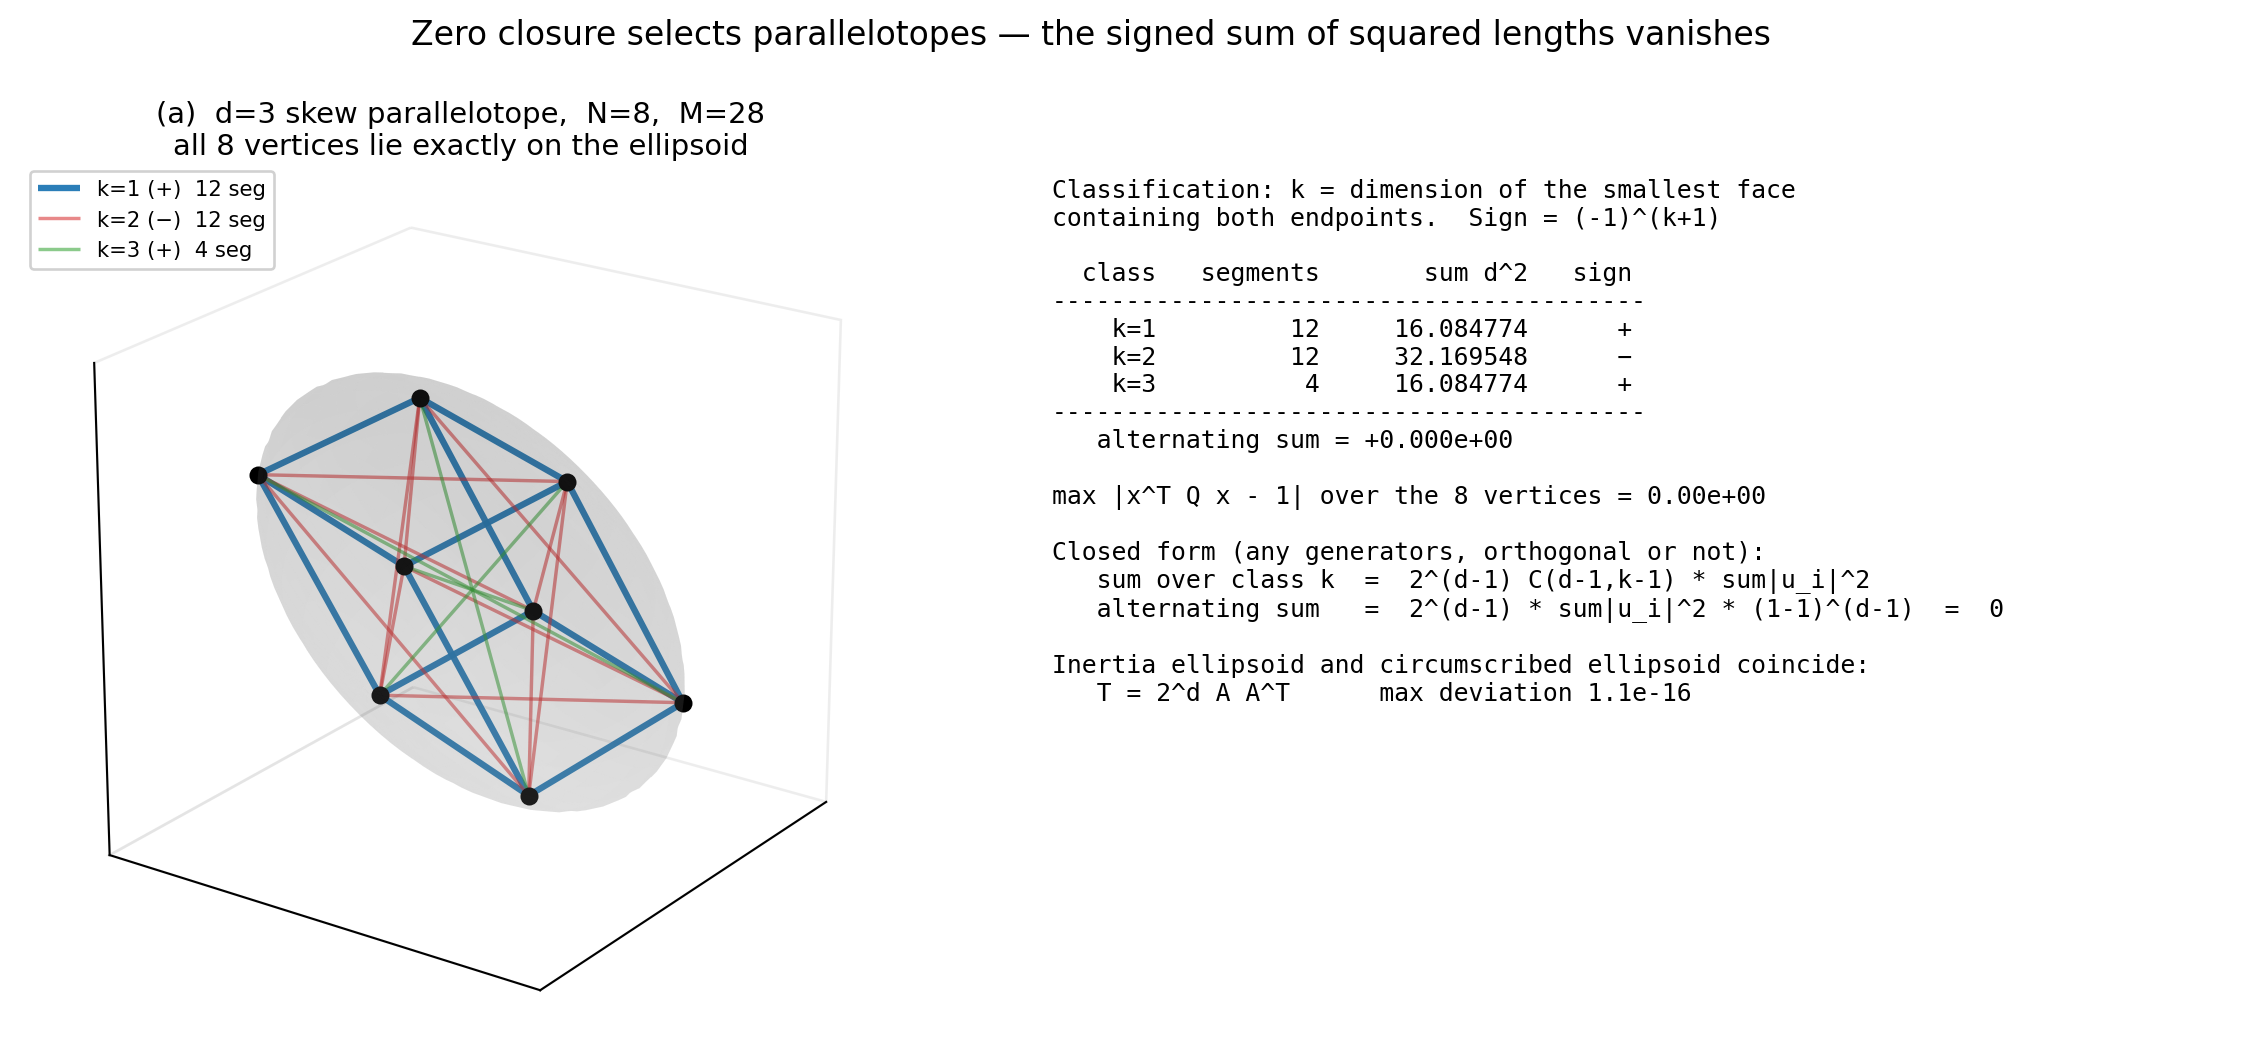
\includegraphics[keepaspectratio,alt={図1}]{figures_v1/fig1_parallelotope_d3.png}}
\caption{図1}
\end{figure}

斜交した平行六面体（\(d = 3\)、\(N = 2^3 = 8\)、\(M = 28\)）。\(28\)
本の線分を、両端点を含む最小の面の次元 \(k\)
で色分けする。\(k=1\)（辺）が12本、\(k=2\)（面の対角線）が12本、\(k=3\)（空間対角線）が4本。符号
\((-1)^{k+1}\) を付けた交代和が厳密に零になる。

\textbf{長さで分類してはならない。}
斜交した平行六面体では相異なる長さ\(^2\)
が13種類現れるが、面次元による分類はちょうど3種類である。立方体のように対称性の高い図形でのみ両者がたまたま一致する。

\paragraph{図2 ---
4次元の平行多面体（3次元への射影）}\label{ux56f32-4ux6b21ux5143ux306eux5e73ux884cux591aux9762ux4f533ux6b21ux5143ux3078ux306eux5c04ux5f71}

\begin{figure}
\centering
\pandocbounded{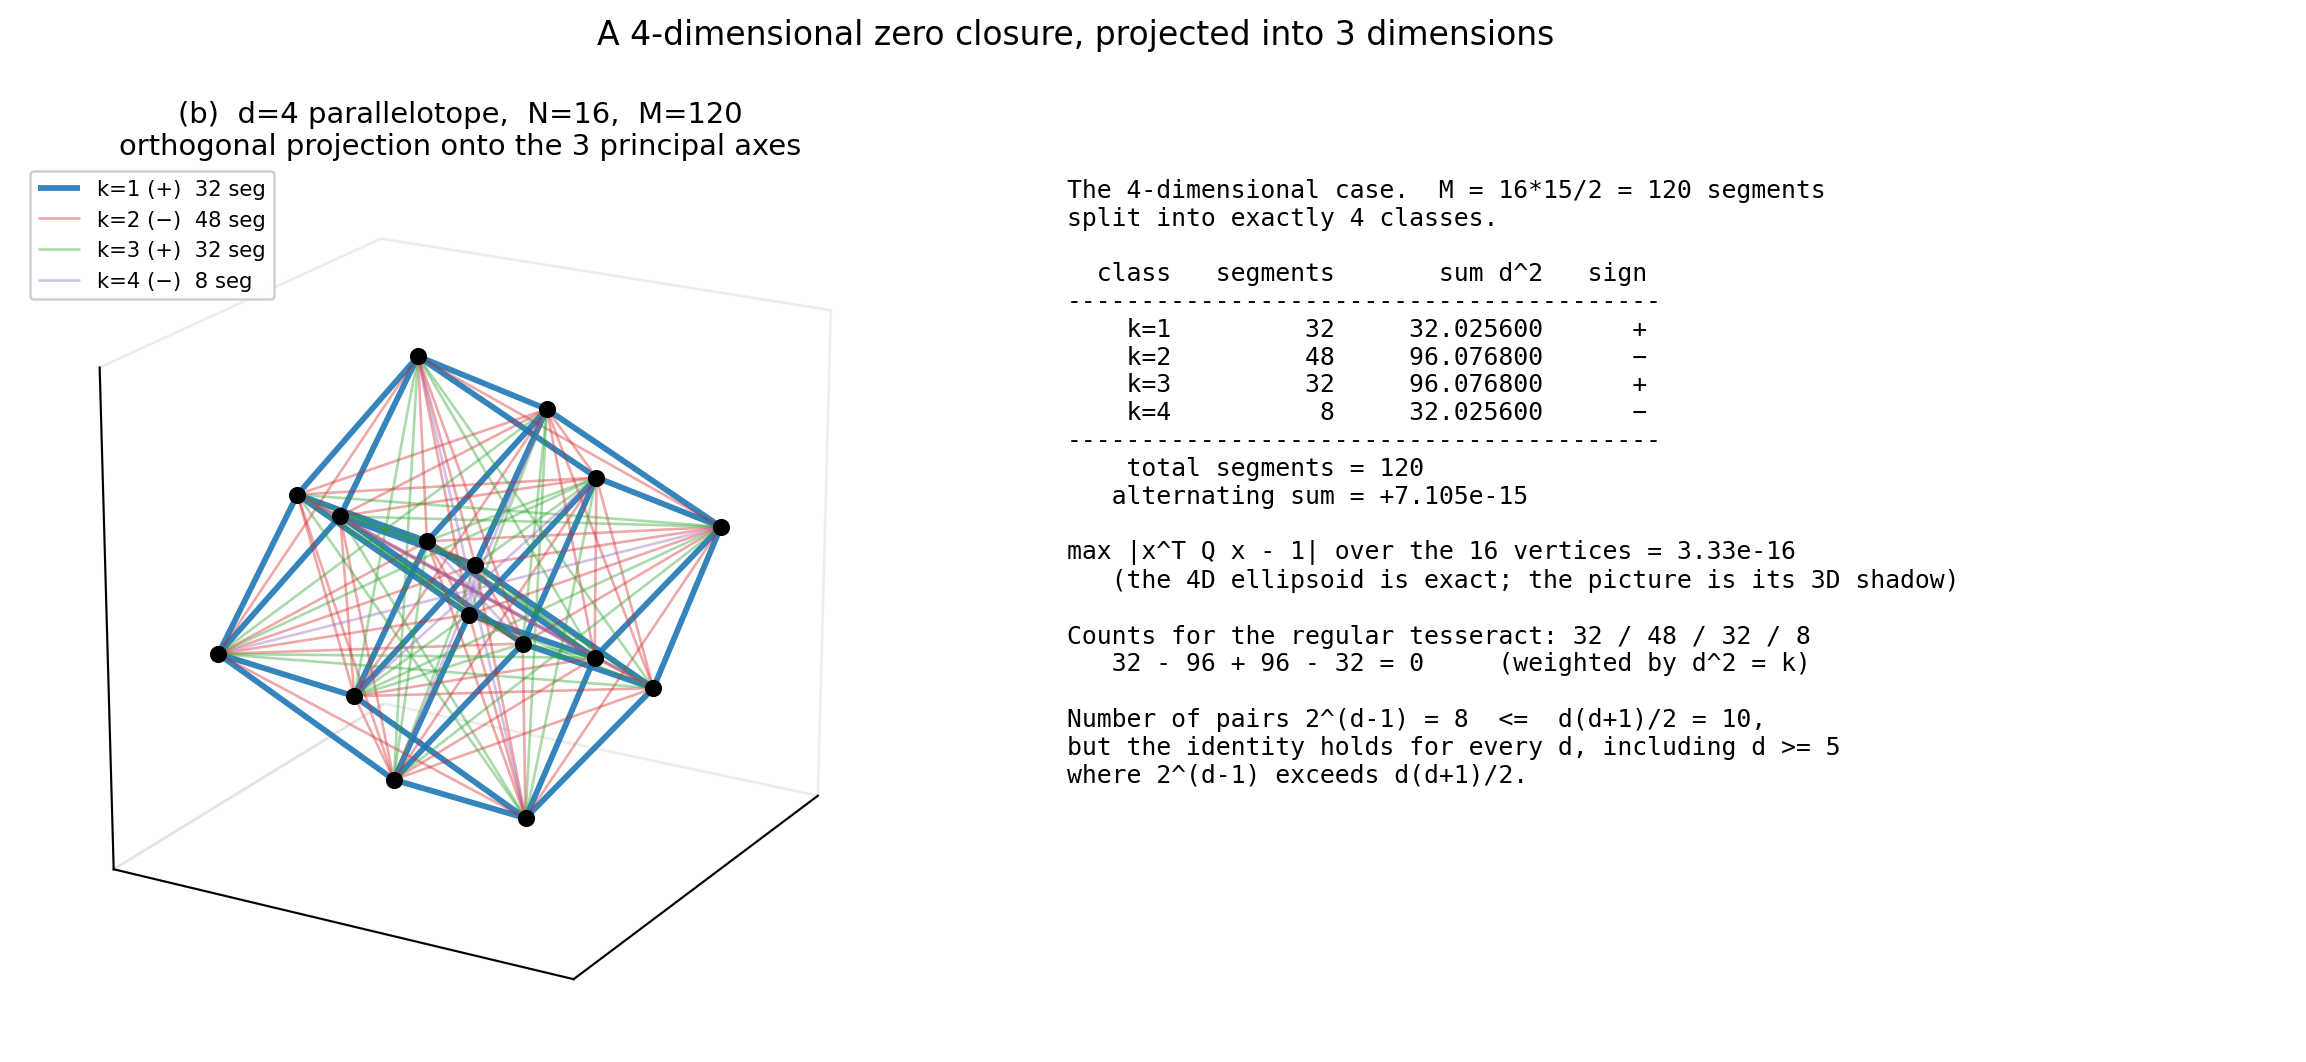
\includegraphics[keepaspectratio,alt={図2}]{figures_v1/fig2_parallelotope_d4_projection.png}}
\caption{図2}
\end{figure}

\(d = 4\)、\(N = 16\)、\(M = 120\)。\(120\)
本が4クラスに分かれる（\(32 / 48 / 32 / 8\)）。\(\sum d^2\) は
\(32.03 / 96.08 / 96.08 / 32.03\) で、交代和は \(+7.1\times10^{-15}\)。

\textbf{絵は3次元への影である。楕円体は4次元では厳密であり、\(16\)
頂点全てで \(|x^{\mathsf T}Qx - 1| \le 3.3\times10^{-16}\)
が成立している。}
影の見た目が楕円からずれて見えても、それは射影の効果である。

対の数は \(2^{d-1} = 8 \le d(d+1)/2 = 10\) であるが、この恒等式は
\(2^{d-1}\) が \(d(d+1)/2\) を超える \(d \ge 5\)
でも成立する（主張6B）。

\paragraph{図3 ---
反例：楕円体に乗るだけでは足りない}\label{ux56f33-ux53cdux4f8bux6955ux5186ux4f53ux306bux4e57ux308bux3060ux3051ux3067ux306fux8db3ux308aux306aux3044}

\begin{figure}
\centering
\pandocbounded{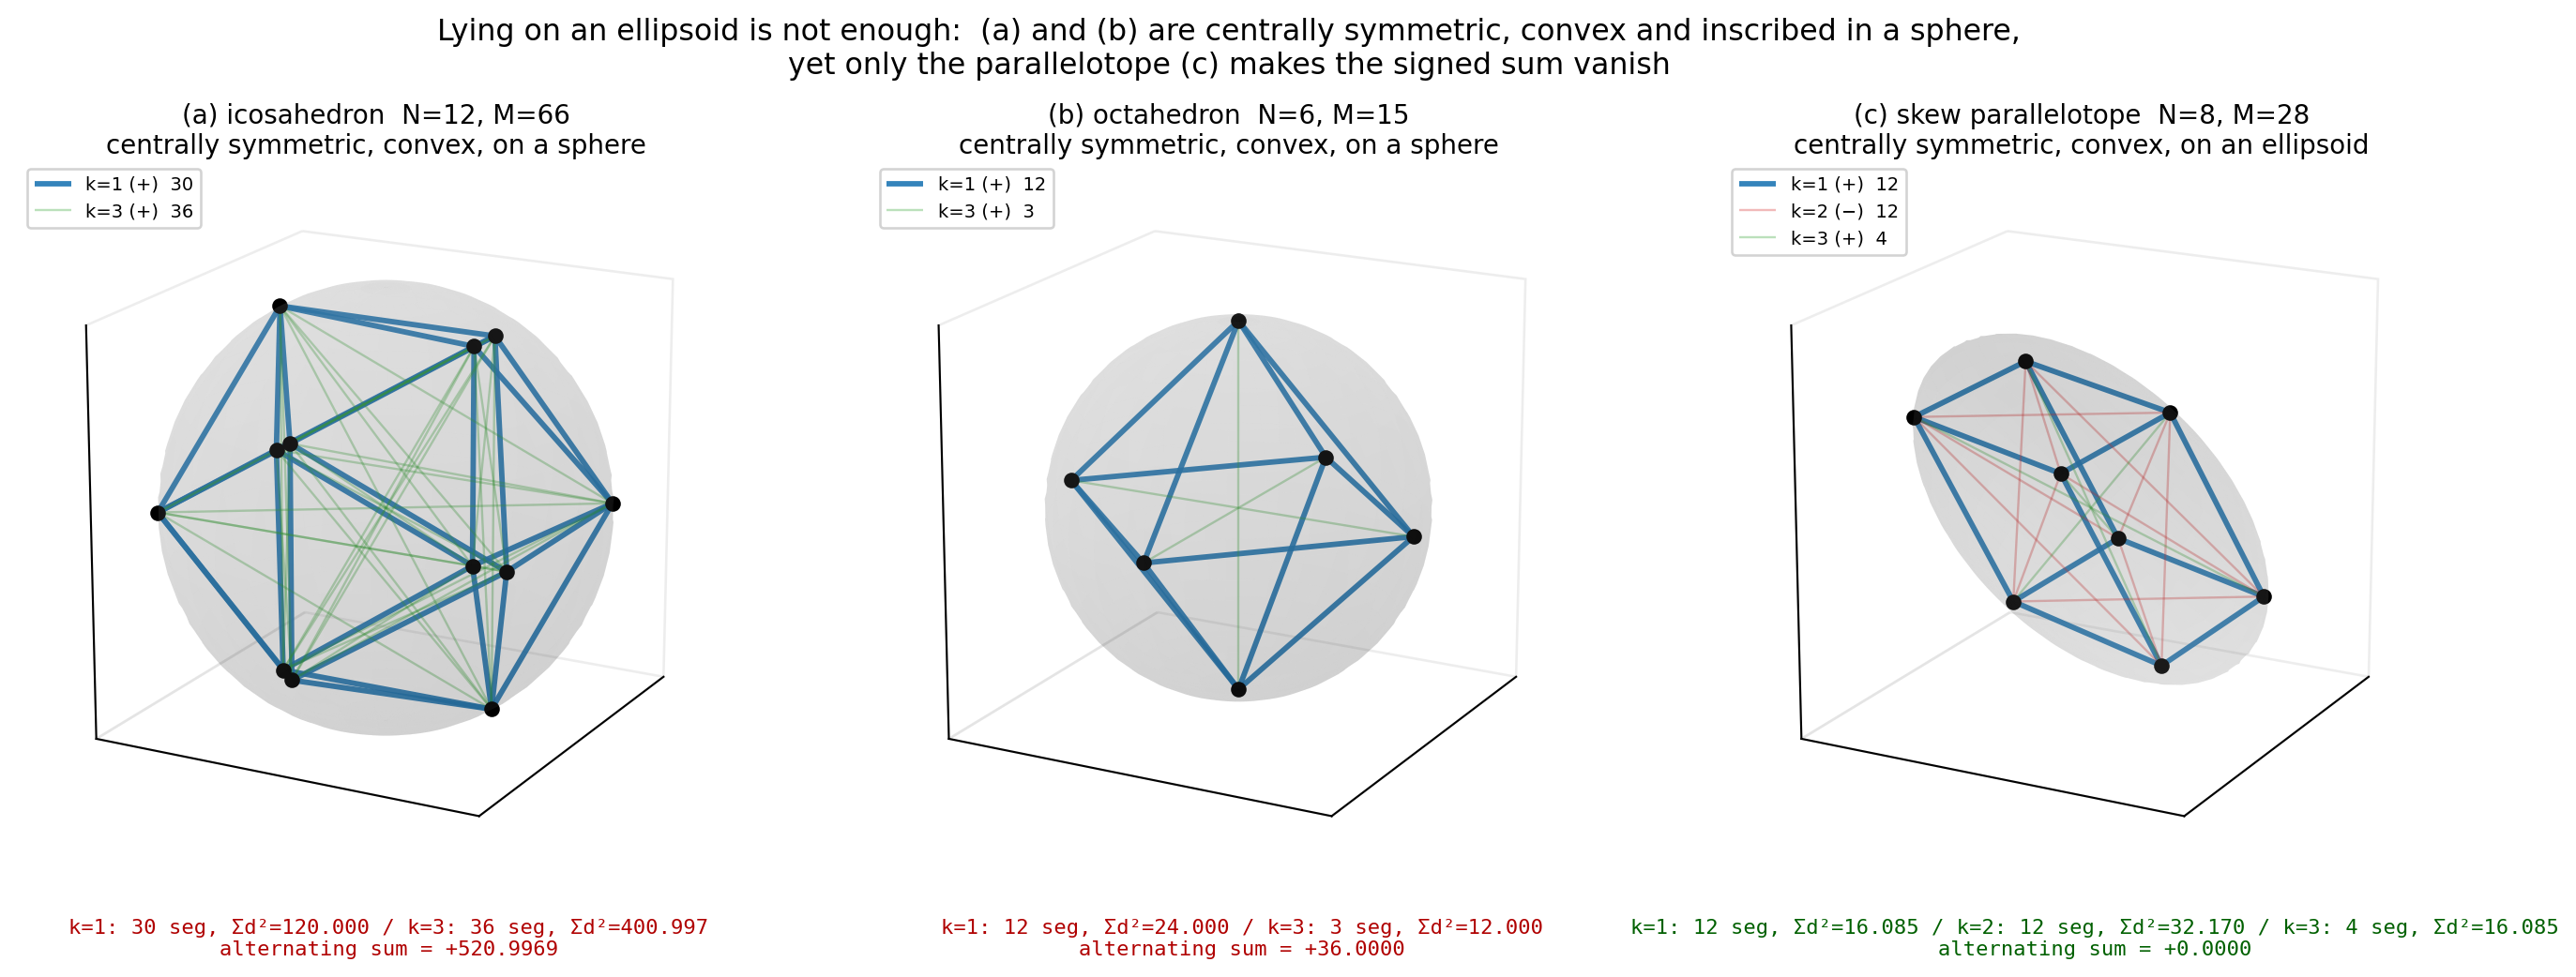
\includegraphics[keepaspectratio,alt={図3}]{figures_v1/fig3_counterexamples.png}}
\caption{図3}
\end{figure}

\begin{enumerate}
\def\labelenumi{(\alph{enumi})}
\tightlist
\item
  正二十面体（\(N=12\)）、(b) 正八面体（\(N=6\)）、(c)
  斜交平行六面体（\(N=8\)）。(a) と (b)
  は\textbf{中心対称かつ凸で、しかも球面上に乗っている}。それでも交代和は
  \(+520.997\) と \(+36.000\) であって零にならない。零になるのは (c)
  の平行多面体だけである（\(+0.0000\)）。
\end{enumerate}

\textbf{この図が示すのは、「楕円面に乗ること」と「零閉鎖すること」は別の条件だという一点である。}
零閉鎖の方が真に強い。

\paragraph{図4 ---
零閉鎖の楕円体と、閉鎖が固定するもの}\label{ux56f34-ux96f6ux9589ux9396ux306eux6955ux5186ux4f53ux3068ux9589ux9396ux304cux56faux5b9aux3059ux308bux3082ux306e}

\begin{figure}
\centering
\pandocbounded{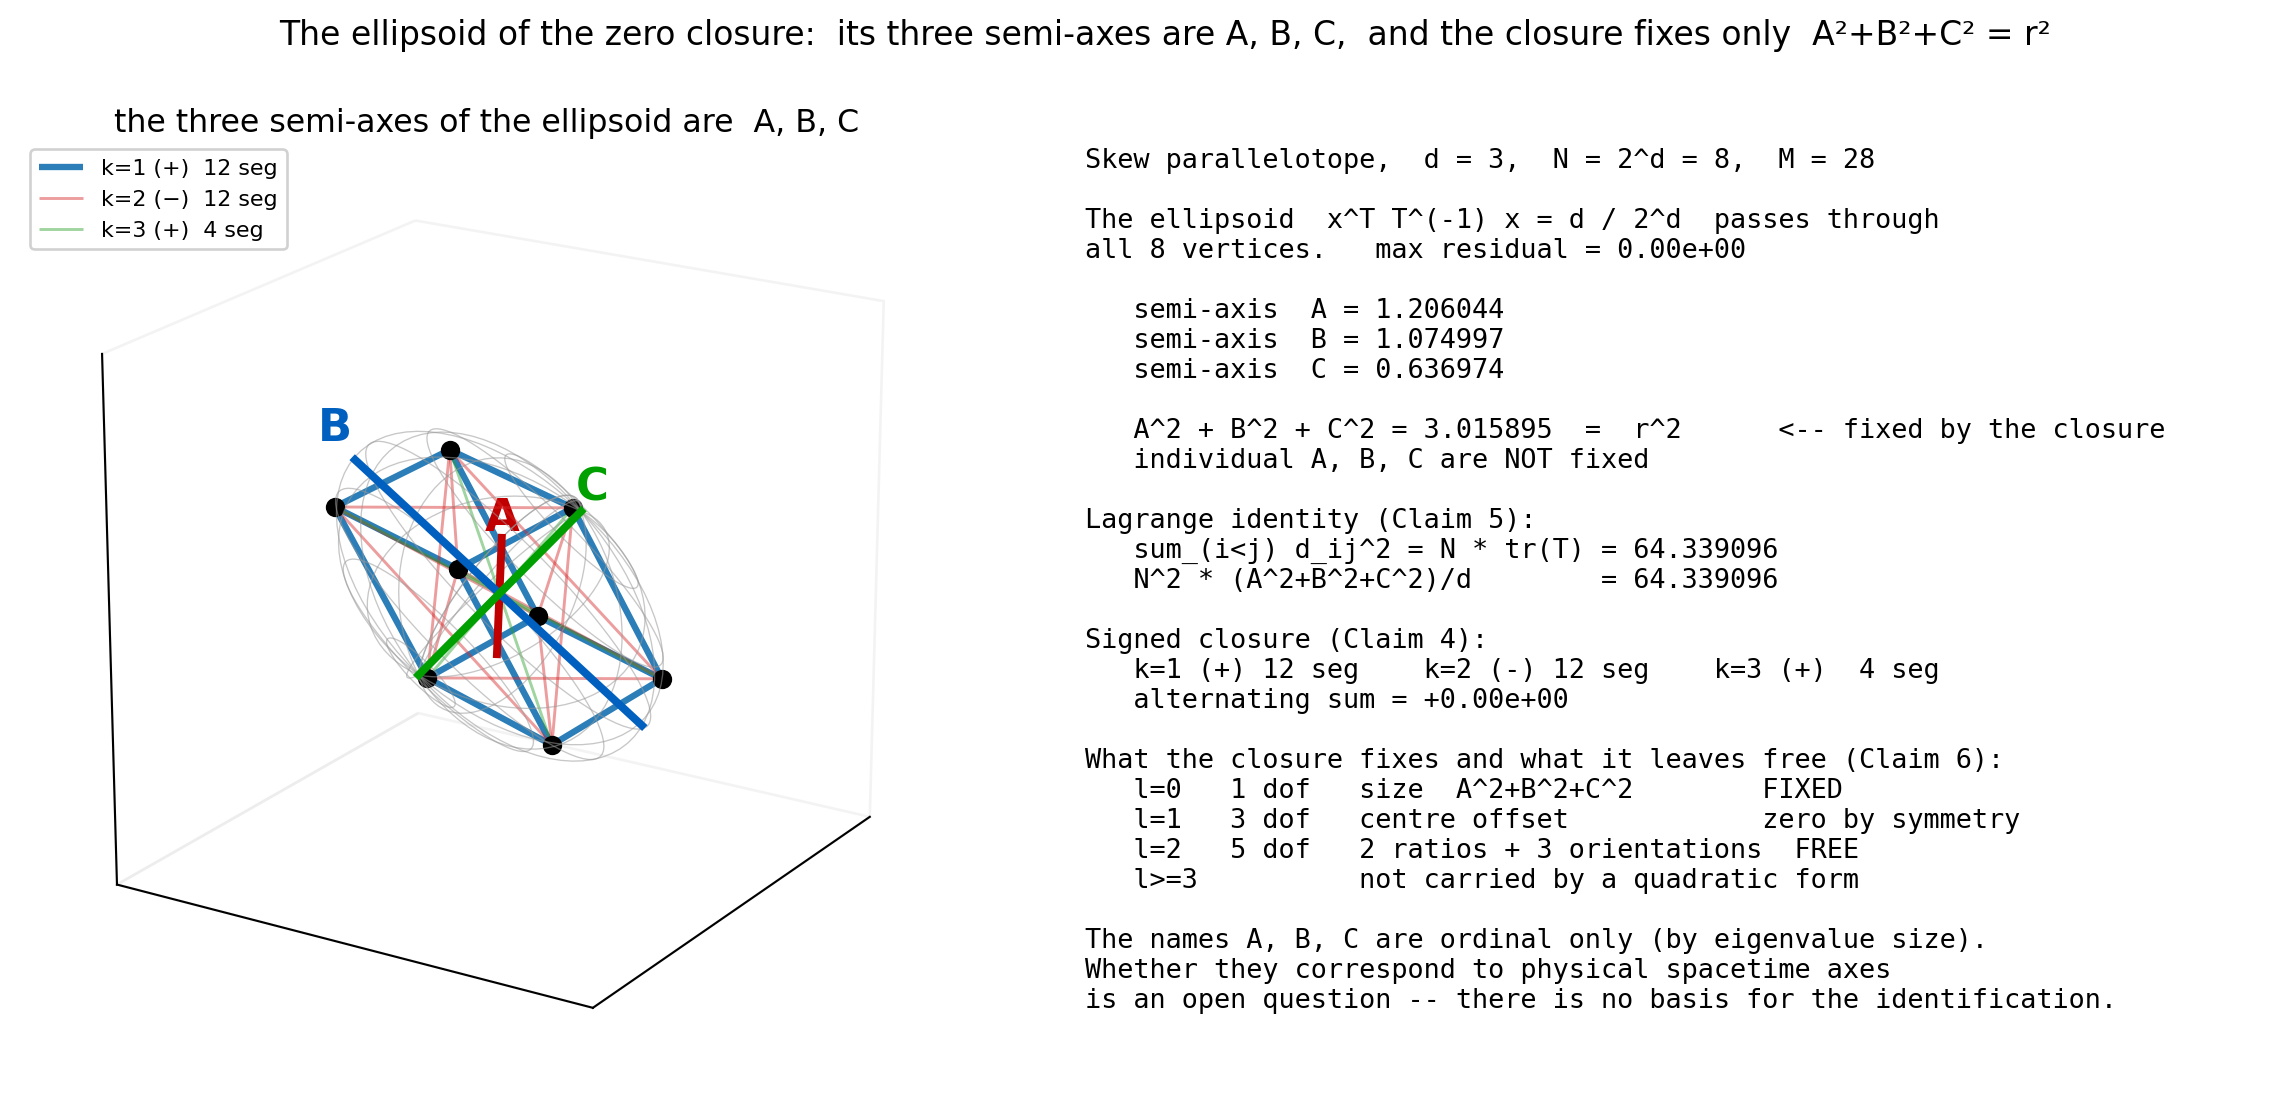
\includegraphics[keepaspectratio,alt={図4}]{figures_v1/fig4_semiaxes_ABC.png}}
\caption{図4}
\end{figure}

平行多面体の外接楕円体は\textbf{正規化慣性楕円体（\(c = d/N\)）}と一致する（主張6B、§0
用語定義）。半軸を \(A, B, C\) とする。\textbf{零閉鎖 \(S(D)=0\)
は符号付き距離和に1条件を課すが、\(A^2+B^2+C^2\) の値は固定しない。}
\(C\) の固定または正規化を加えると無符号全二乗量 \(U(D)=2C\)
が固定され、それに対応して慣性テンソルのトレース、すなわち \(l=0\)
が固定される（主張5）。個々の \(A, B, C\) は決まらない。多重極で分けると
\(l=0\) の1自由度が（\(C\) 固定または正規化により）決まり、\(l=2\)
の5自由度（形2＋向き3）が自由に残る（主張6）。\textbf{\(T\) の分解は
\(l=0\oplus l=2\) の二つだけであり、\(l=1\)（一次モーメント）は \(T\)
の成分ではない。重心座標では定義により零である}（主張6 の訂正）。

\(A, B, C\)
という名前は固有値の大小順で付けた序数である。物理的時空との対応は今後の課題である（§0B、主張12）。

\subsubsection{5.2
数値模型の図（走行結果）}\label{ux6570ux5024ux6a21ux578bux306eux56f3ux8d70ux884cux7d50ux679c}

条件：mode =
electron、\(N = 16 = 2^4\)、\(\delta = 0.1\)、\(T = 40000\)。物質側（\texttt{\_m\_}）と真空対照（\texttt{\_v\_}）。各図は4段構成である。

{\def\LTcaptype{none} % do not increment counter
\begin{longtable}[]{@{}
  >{\raggedright\arraybackslash}p{(\linewidth - 2\tabcolsep) * \real{0.5000}}
  >{\raggedright\arraybackslash}p{(\linewidth - 2\tabcolsep) * \real{0.5000}}@{}}
\toprule\noalign{}
\begin{minipage}[b]{\linewidth}\raggedright
段
\end{minipage} & \begin{minipage}[b]{\linewidth}\raggedright
内容
\end{minipage} \\
\midrule\noalign{}
\endhead
\bottomrule\noalign{}
\endlastfoot
(a) & 絶対スケール。枠は \(\pm 0.17\) に固定。全 \(\tau\)
で同じ枠なので、枠に対する大きさの変化がそのままスケールの変化である \\
(b) & \(r_{\rm rms}\) で正規化。枠は \(\pm 1.1\)
に固定。形だけを比較する \\
(c) & スケール履歴（対数）。現在の \(\tau\) を縦線で示す \\
(d) & 全15主軸の履歴。\(0\) より上が実、下が虚 \\
\end{longtable}
}

\begin{quote}
\textbf{枠の値について（v3 の記述誤りの訂正）}：図の題字に出る
\texttt{half-range} は起動引数 \texttt{-\/-absmax}
の値であり、実際の枠はこれを \texttt{-\/-zoom}（既定
2.0）で割った値である。v3 は \(\pm0.28\)／\(\pm2.2\)
と書いていたが、実際の枠は \(\pm0.14\)／\(\pm1.1\) であった。v4 の
\(N=16\) 図は \texttt{-\/-absmax\ 0.34\ -\/-zoom\ 2}（実枠
\(\pm0.17\)）で全頂点が枠内に入るようにしてある。
\end{quote}

頂点の色は偏差
\(s_i\)（青が楕円面の内側、赤が外側、白が楕円面上）、線分の色は関係の長さ
\(|z|\) である。

\paragraph{図5〜8 ---
物質側の4時点}\label{ux56f358-ux7269ux8ceaux5074ux306e4ux6642ux70b9}

{\def\LTcaptype{none} % do not increment counter
\begin{longtable}[]{@{}
  >{\raggedright\arraybackslash}p{(\linewidth - 2\tabcolsep) * \real{0.5000}}
  >{\raggedright\arraybackslash}p{(\linewidth - 2\tabcolsep) * \real{0.5000}}@{}}
\toprule\noalign{}
\begin{minipage}[b]{\linewidth}\raggedright
\(\tau\)
\end{minipage} & \begin{minipage}[b]{\linewidth}\raggedright
図
\end{minipage} \\
\midrule\noalign{}
\endhead
\bottomrule\noalign{}
\endlastfoot
0（開始） &
\pandocbounded{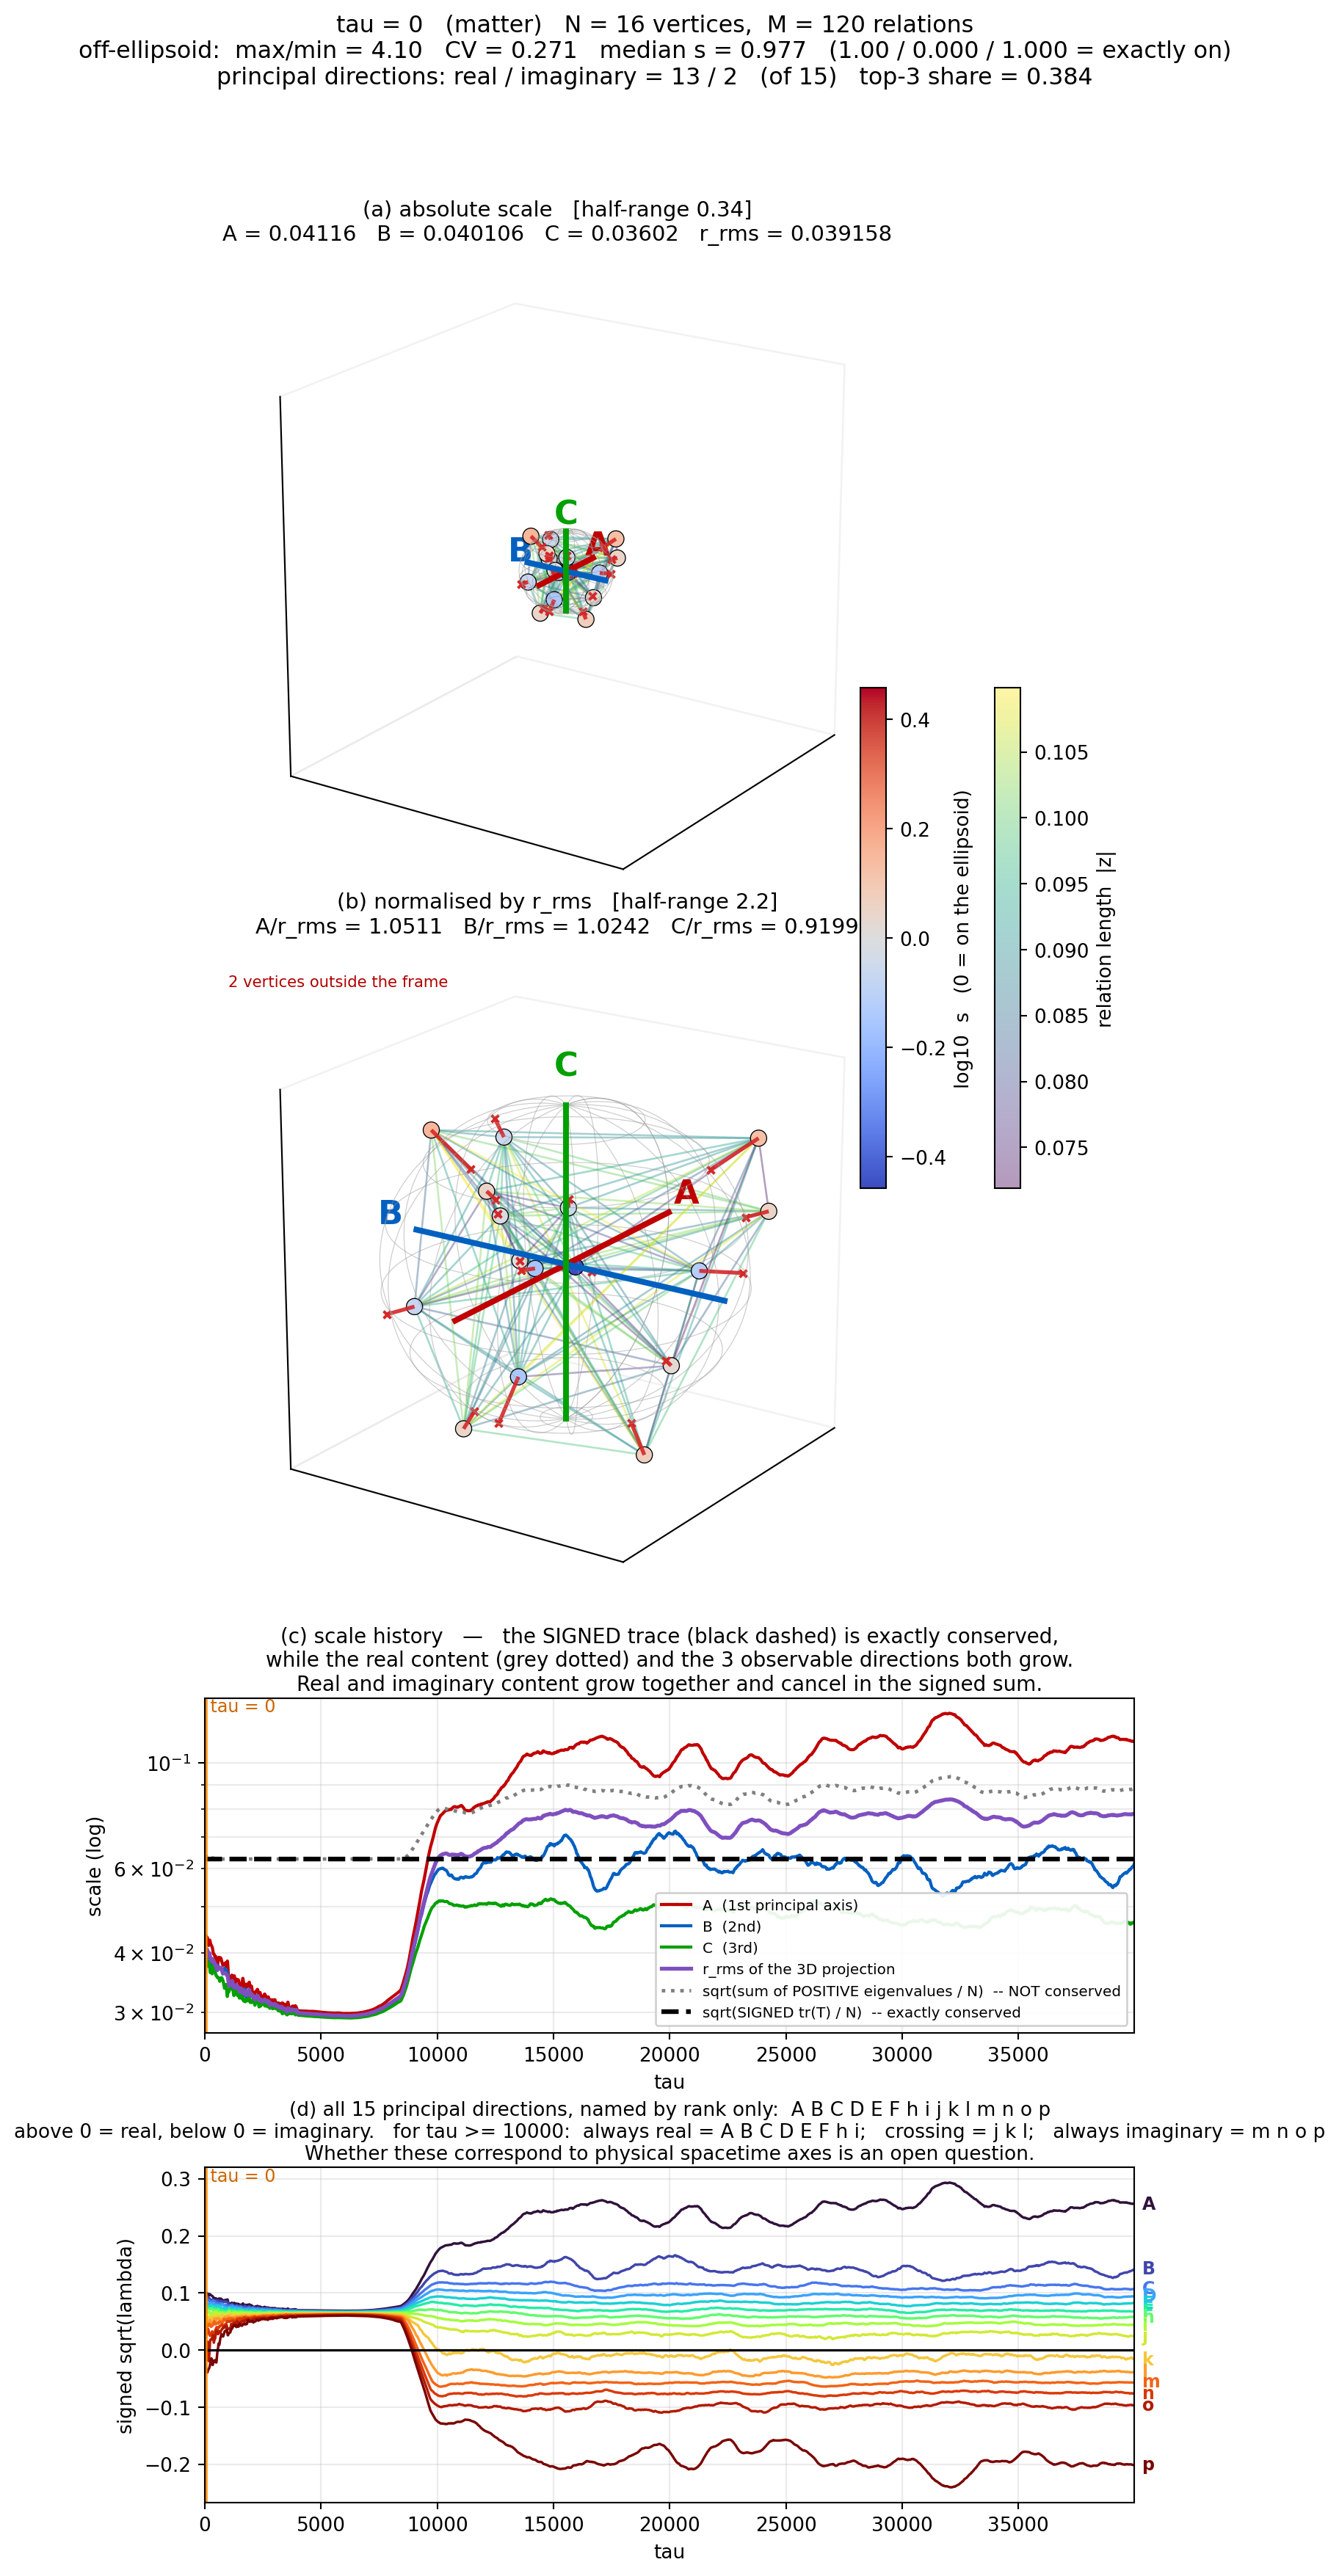
\includegraphics[keepaspectratio,alt={物質 τ=0}]{複製_ダンプ版_v1/次元の生成構造/対照実験_N掃引1to20_三系_v2/figures_tau/fig_ellipsoid_tau00000_electron_T40000_d0.1_rep-dump40k16_N16_m_v1.png}} \\
4000（転移前） &
\pandocbounded{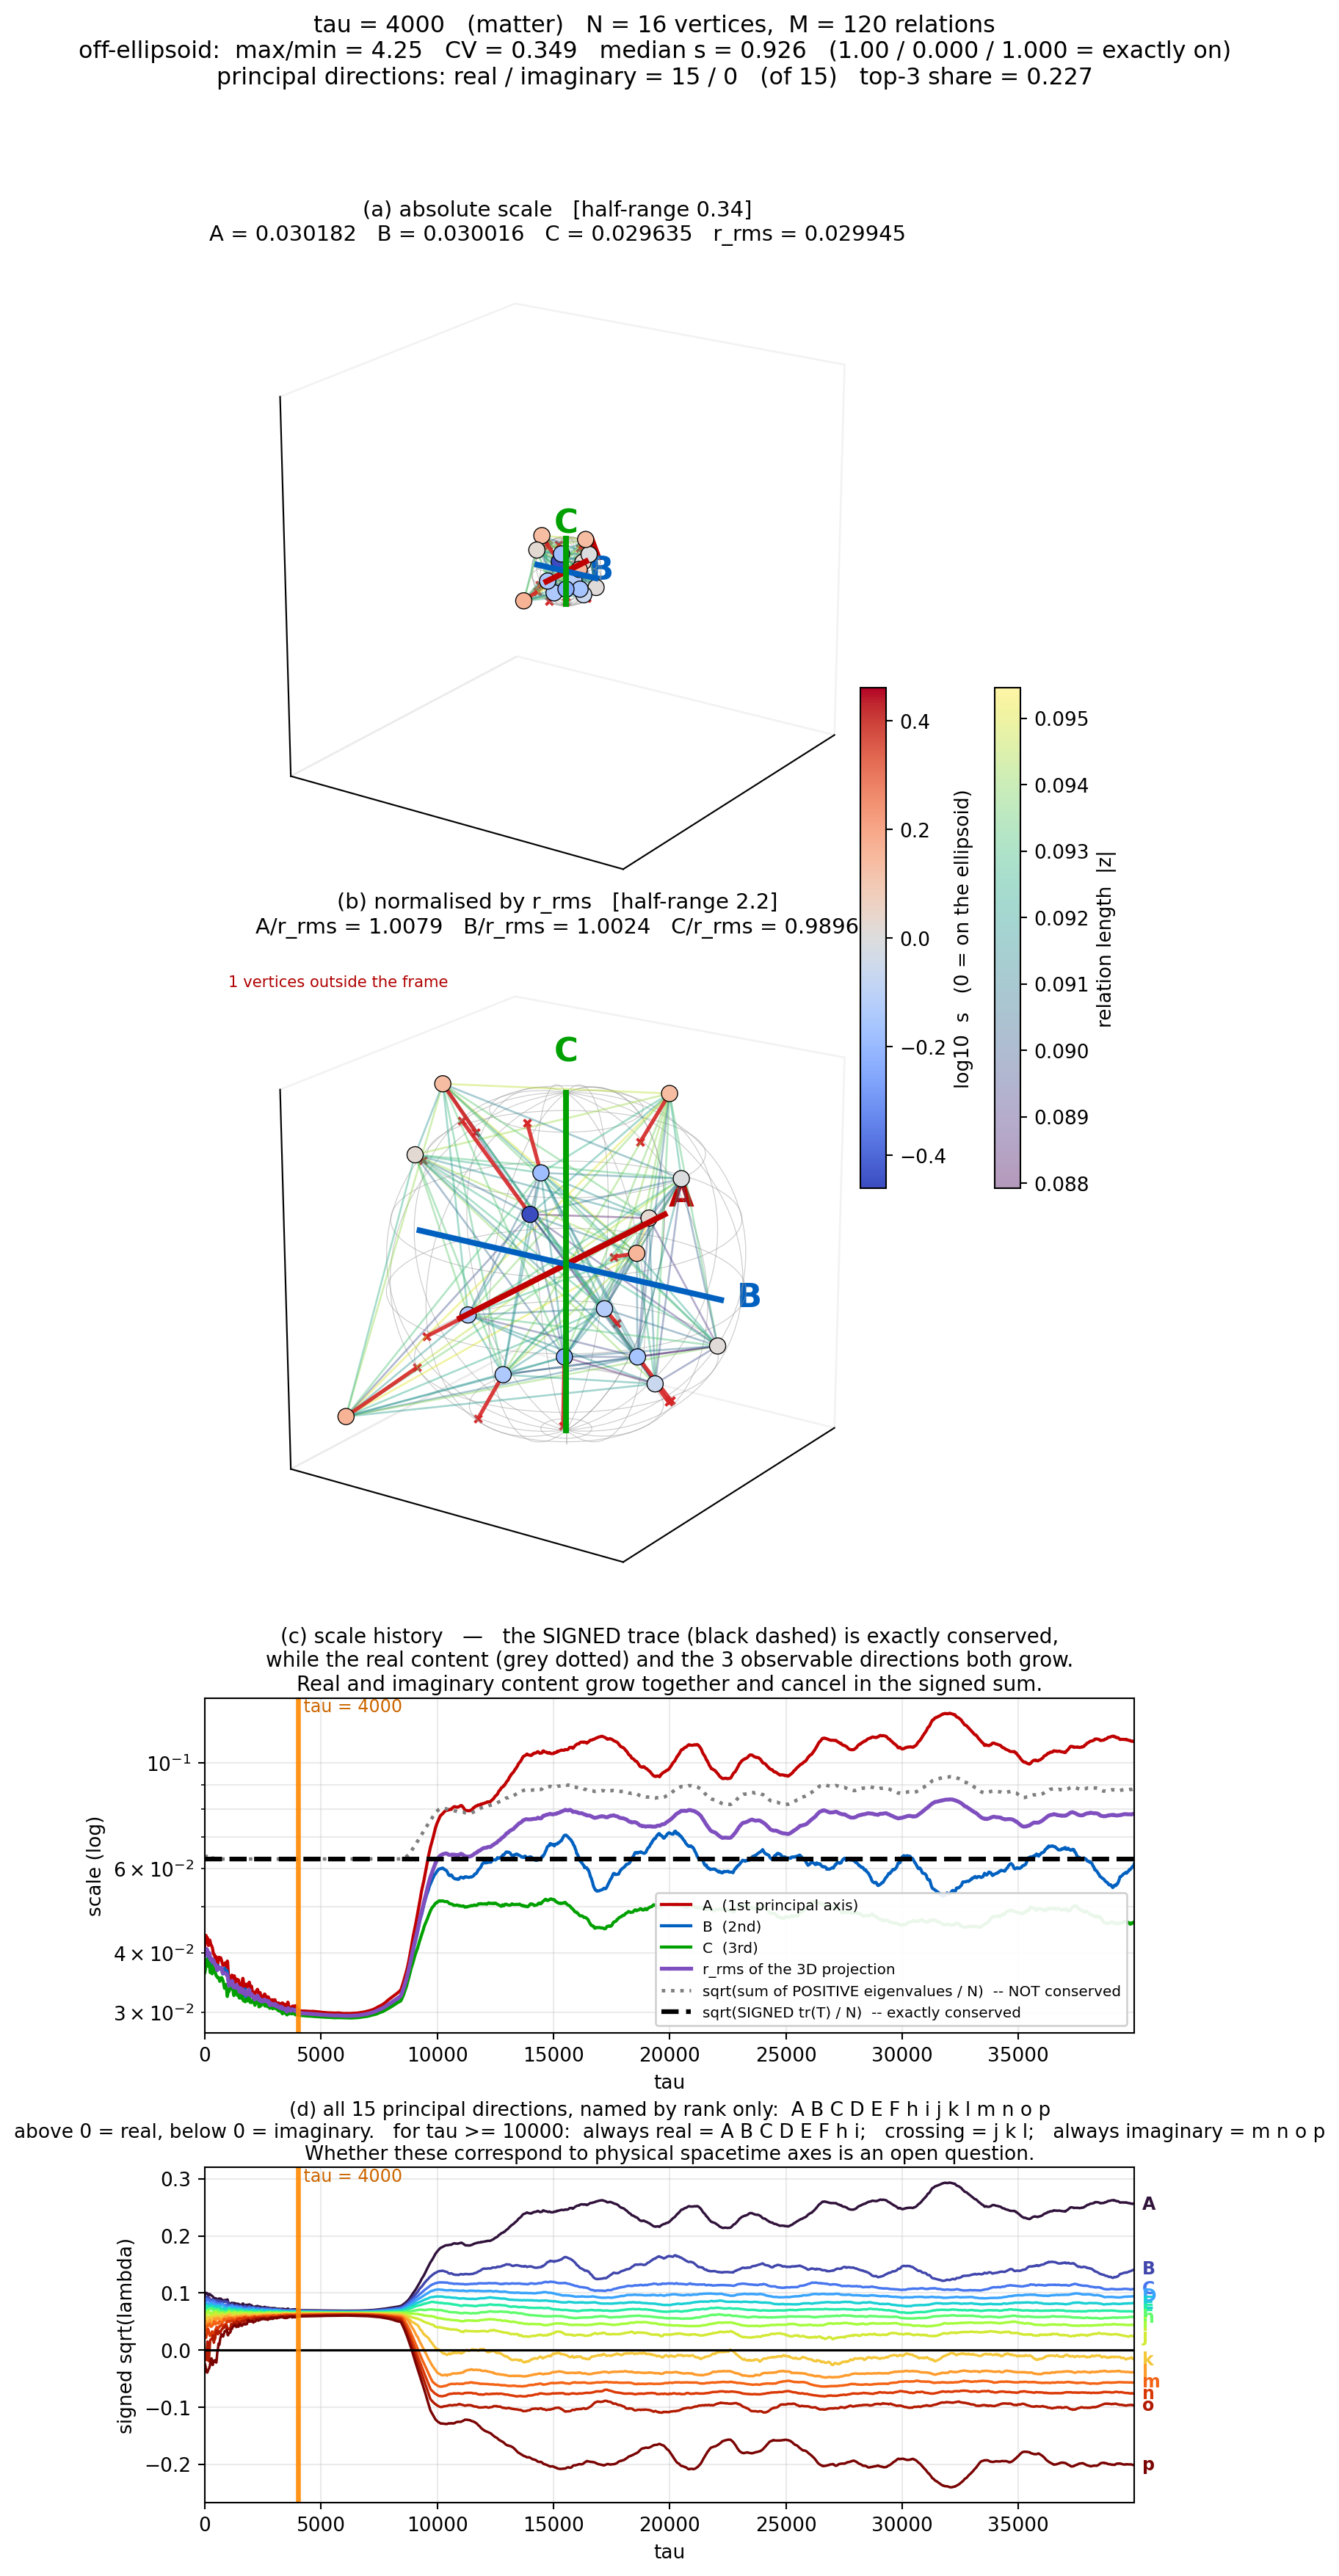
\includegraphics[keepaspectratio,alt={物質 τ=4000}]{複製_ダンプ版_v1/次元の生成構造/対照実験_N掃引1to20_三系_v2/figures_tau/fig_ellipsoid_tau04000_electron_T40000_d0.1_rep-dump40k16_N16_m_v1.png}} \\
9487（転移直後） &
\pandocbounded{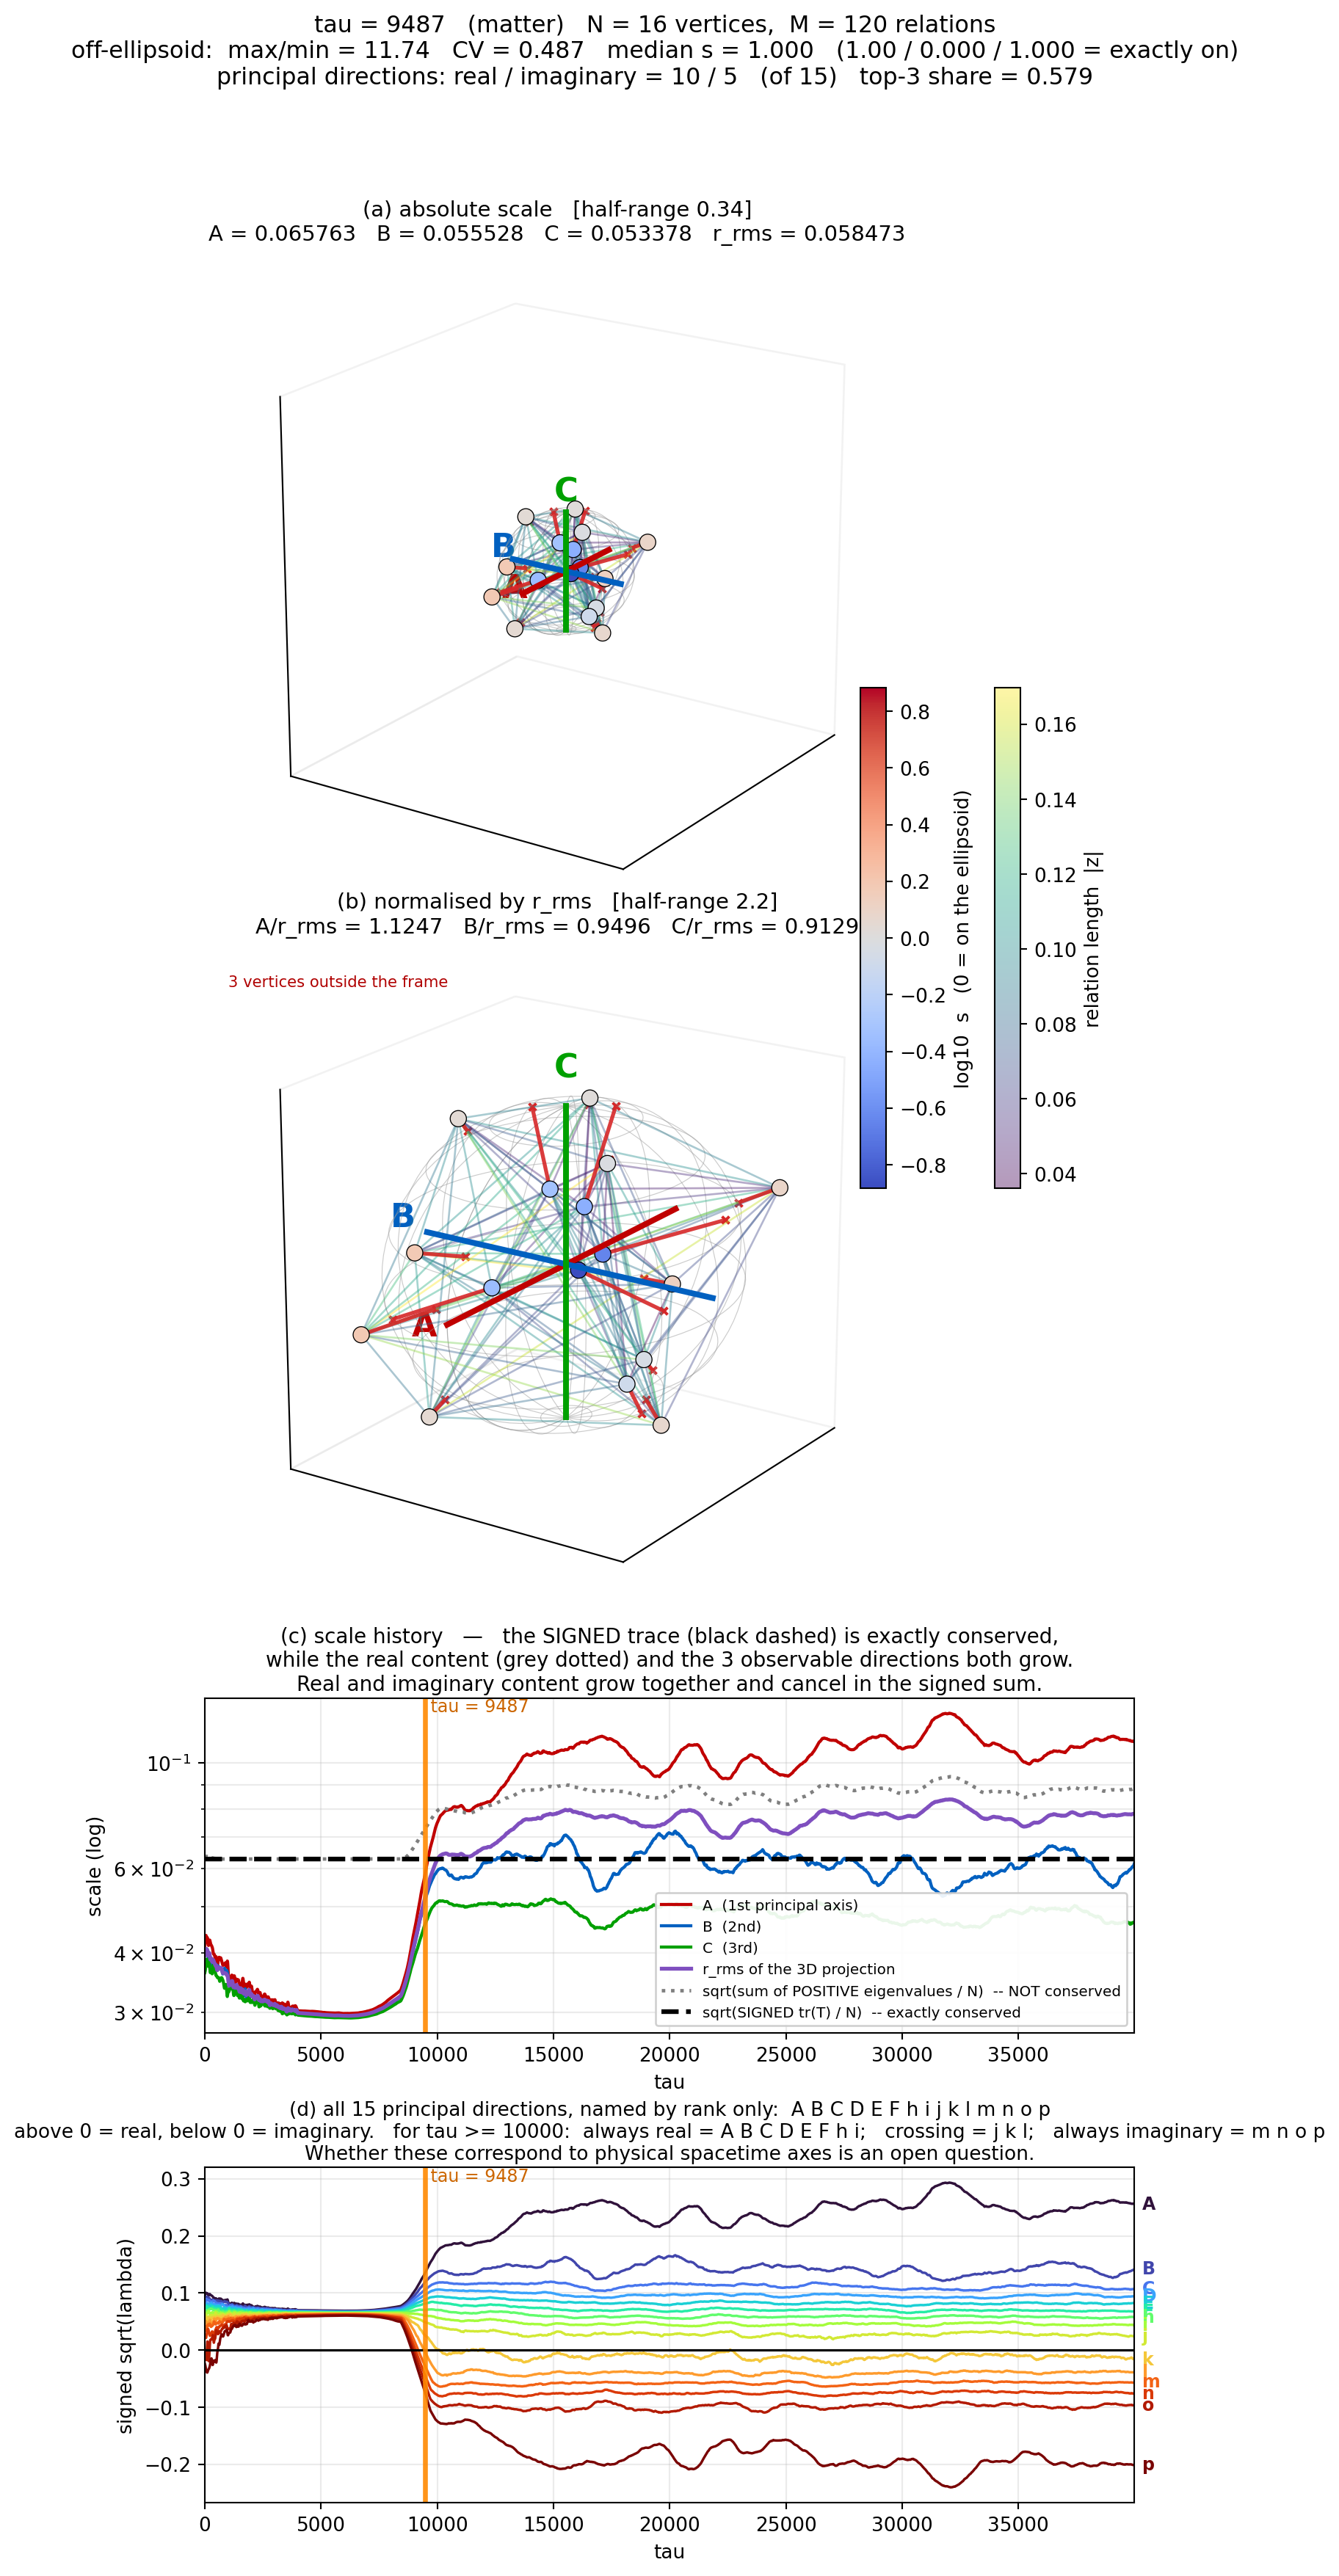
\includegraphics[keepaspectratio,alt={物質 τ=9487}]{複製_ダンプ版_v1/次元の生成構造/対照実験_N掃引1to20_三系_v2/figures_tau/fig_ellipsoid_tau09487_electron_T40000_d0.1_rep-dump40k16_N16_m_v1.png}} \\
39991（終了） &
\pandocbounded{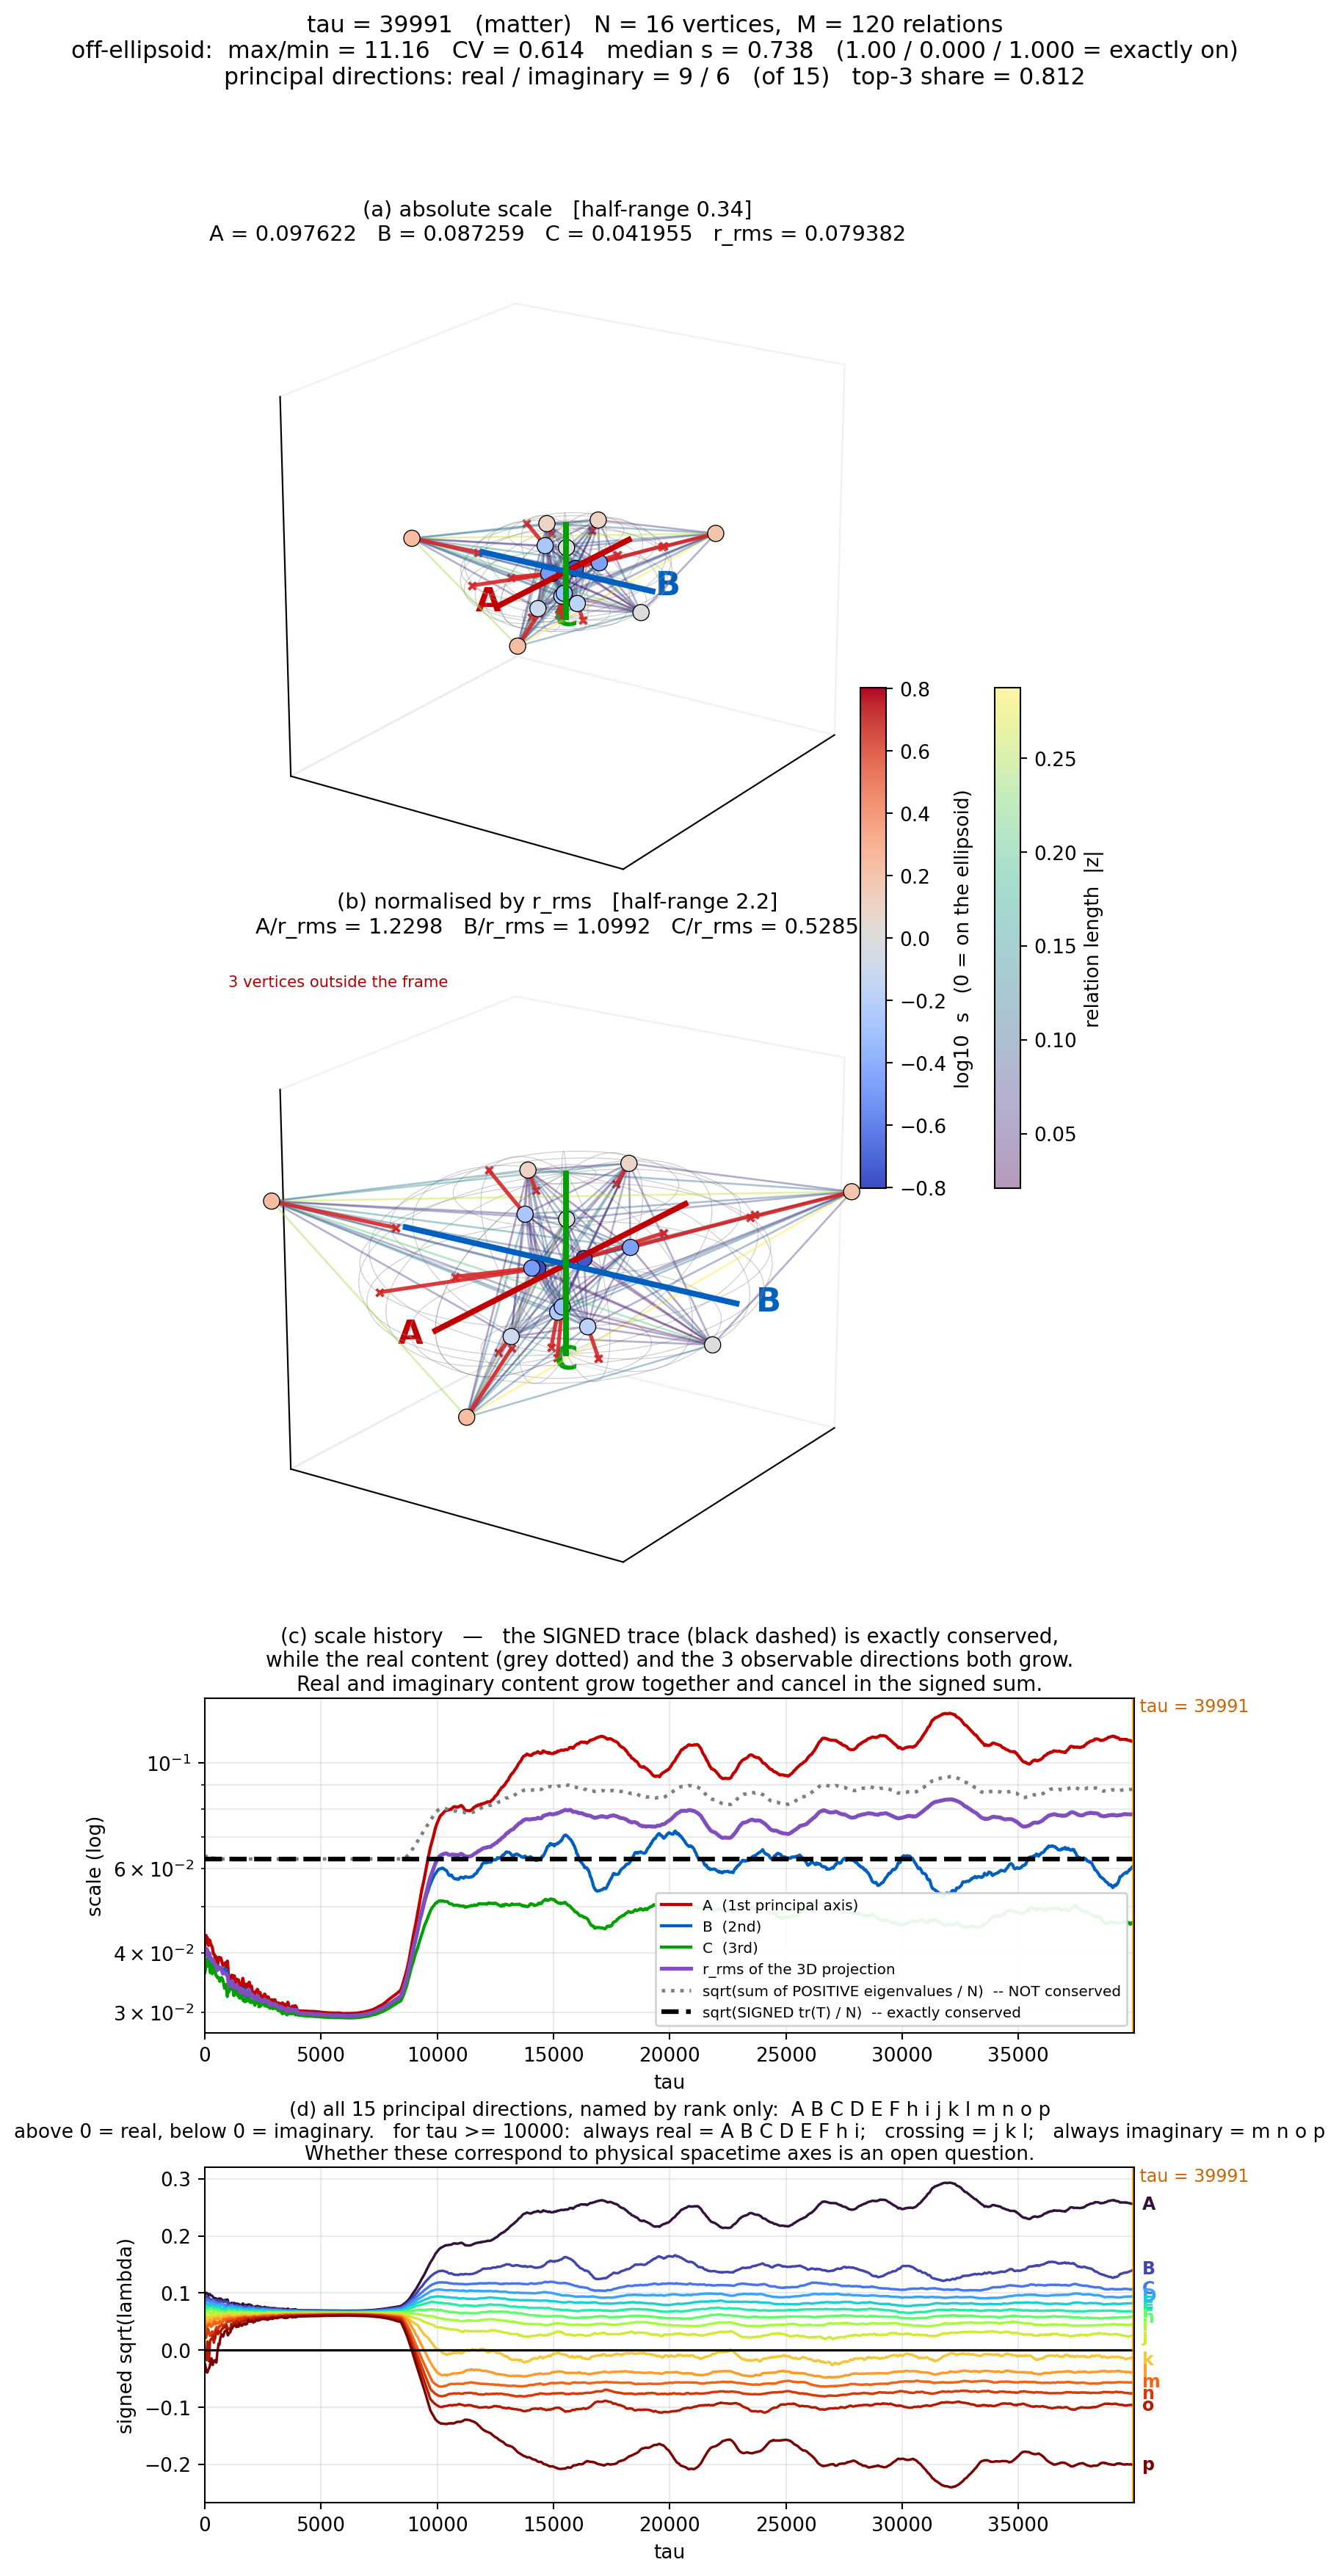
\includegraphics[keepaspectratio,alt={物質 τ=39991}]{複製_ダンプ版_v1/次元の生成構造/対照実験_N掃引1to20_三系_v2/figures_tau/fig_ellipsoid_tau39991_electron_T40000_d0.1_rep-dump40k16_N16_m_v1.png}} \\
\end{longtable}
}

\paragraph{図9〜12 ---
真空対照の4時点}\label{ux56f3912-ux771fux7a7aux5bfeux7167ux306e4ux6642ux70b9}

{\def\LTcaptype{none} % do not increment counter
\begin{longtable}[]{@{}
  >{\raggedright\arraybackslash}p{(\linewidth - 2\tabcolsep) * \real{0.5000}}
  >{\raggedright\arraybackslash}p{(\linewidth - 2\tabcolsep) * \real{0.5000}}@{}}
\toprule\noalign{}
\begin{minipage}[b]{\linewidth}\raggedright
\(\tau\)
\end{minipage} & \begin{minipage}[b]{\linewidth}\raggedright
図
\end{minipage} \\
\midrule\noalign{}
\endhead
\bottomrule\noalign{}
\endlastfoot
0 &
\pandocbounded{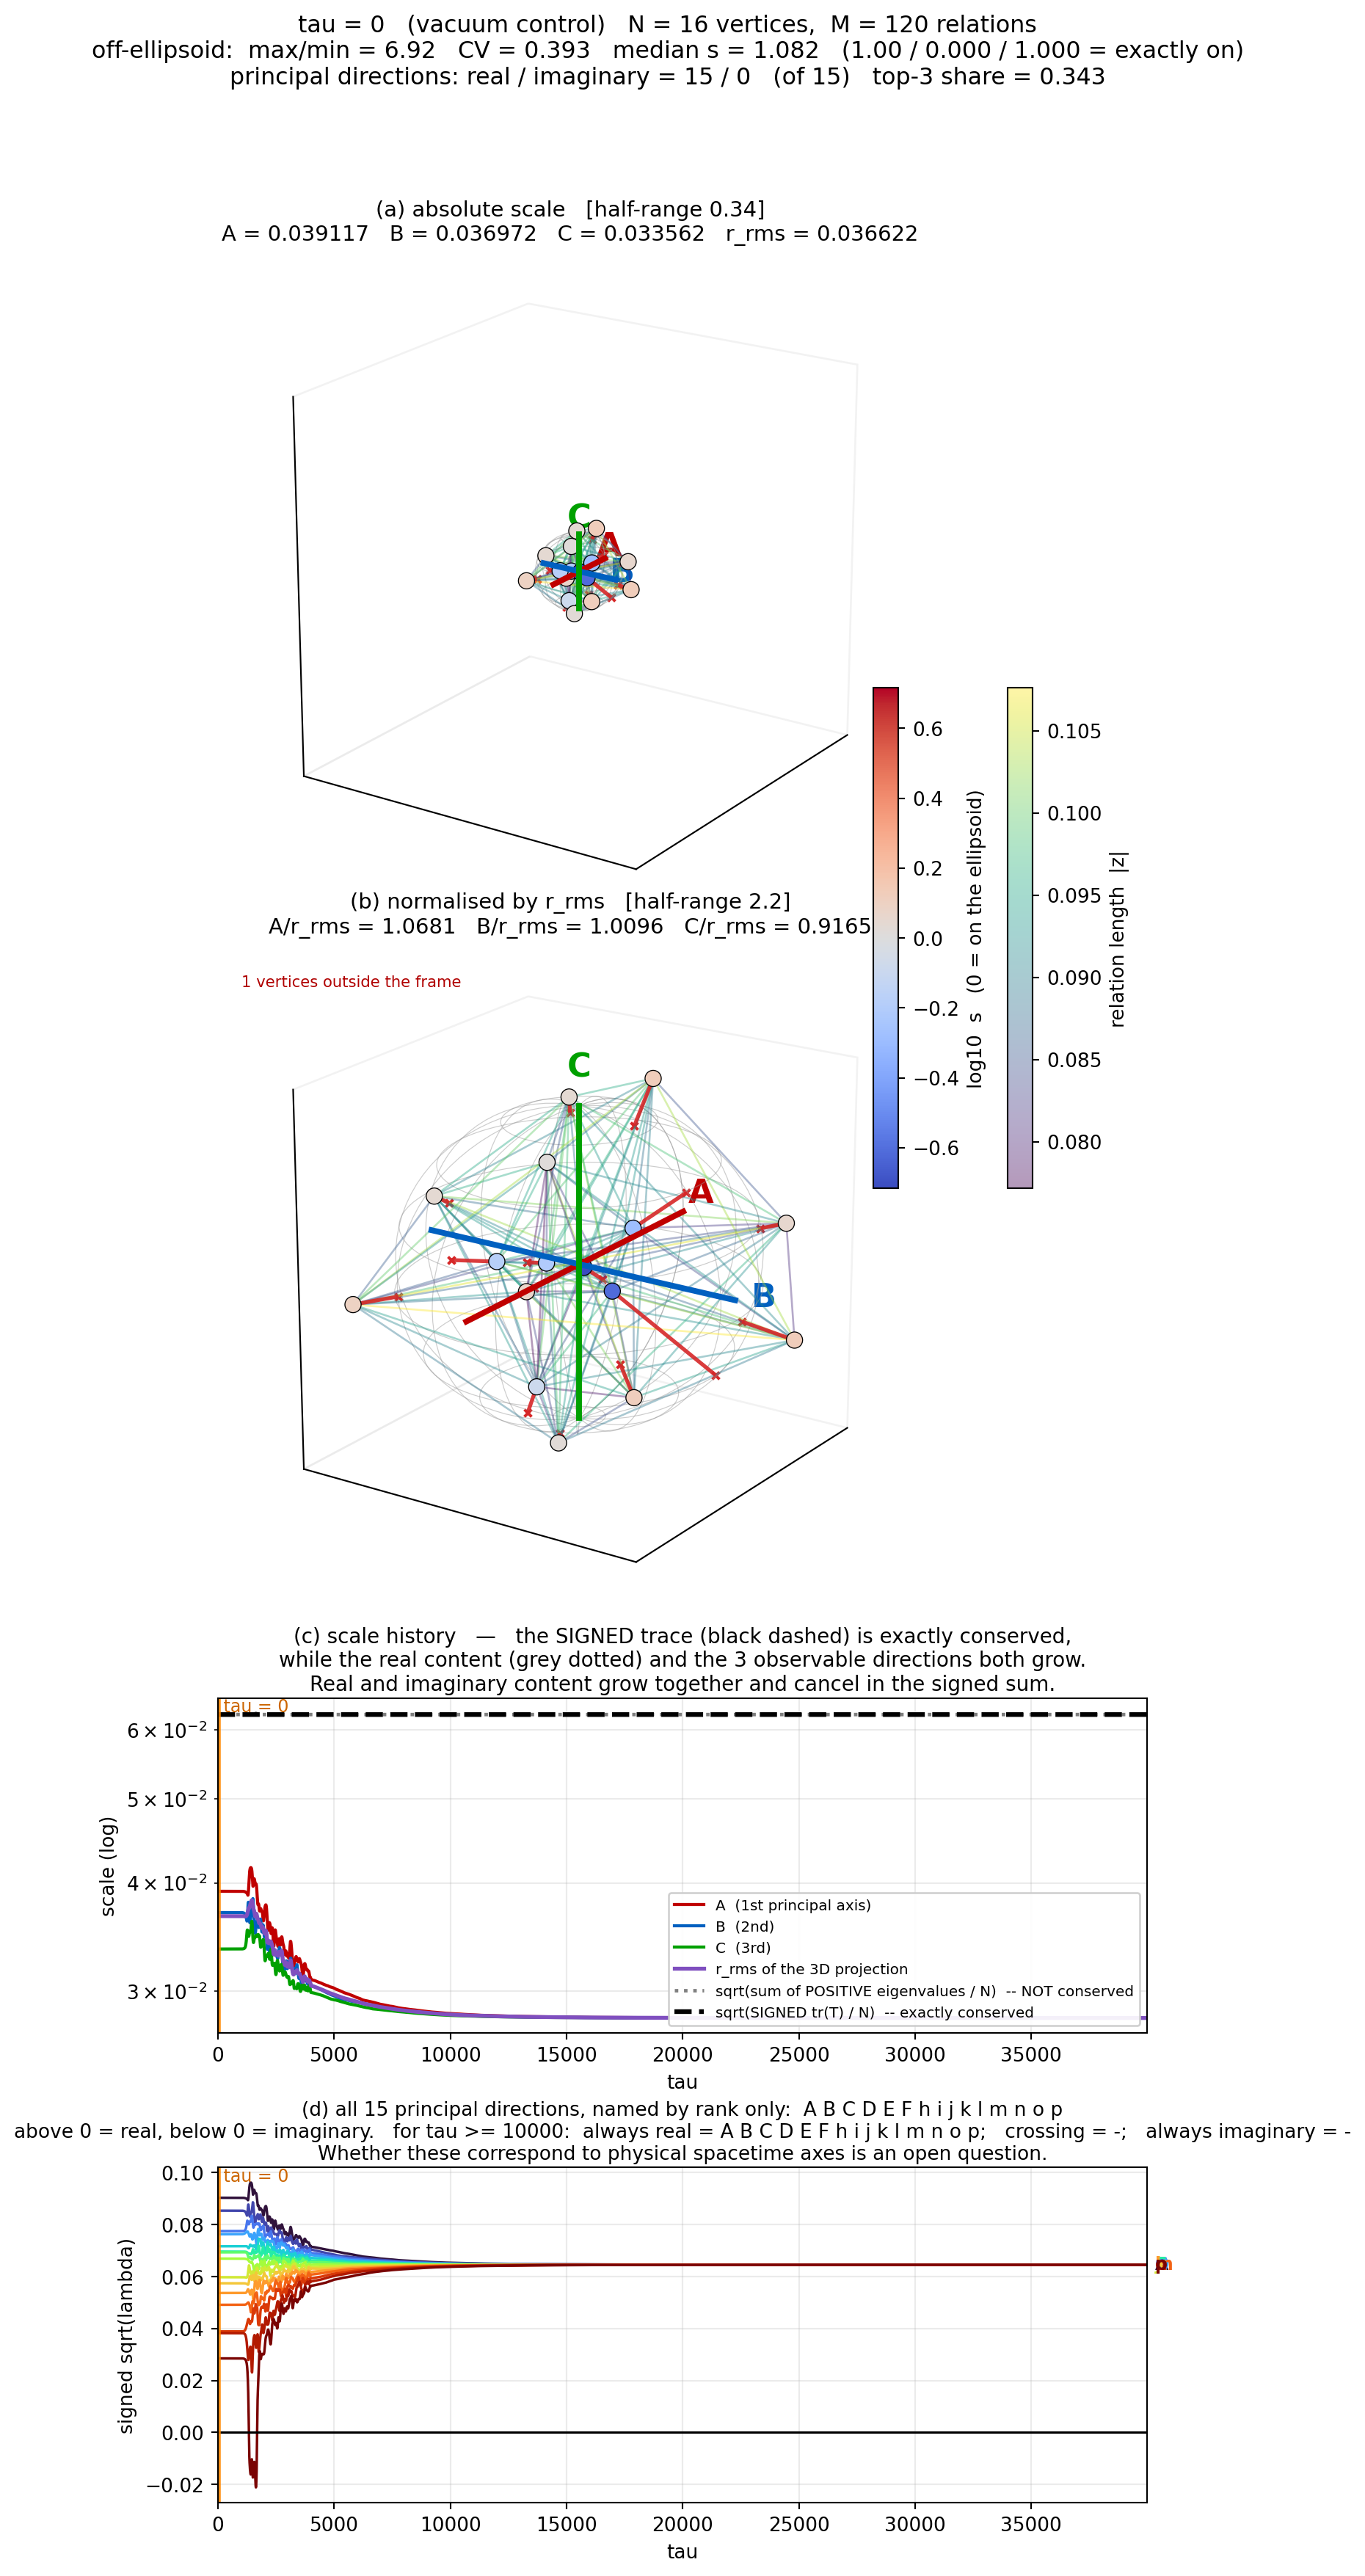
\includegraphics[keepaspectratio,alt={真空 τ=0}]{複製_ダンプ版_v1/次元の生成構造/対照実験_N掃引1to20_三系_v2/figures_tau/fig_ellipsoid_tau00000_electron_T40000_d0.1_rep-dump40k16_N16_v_v1.png}} \\
4000 &
\pandocbounded{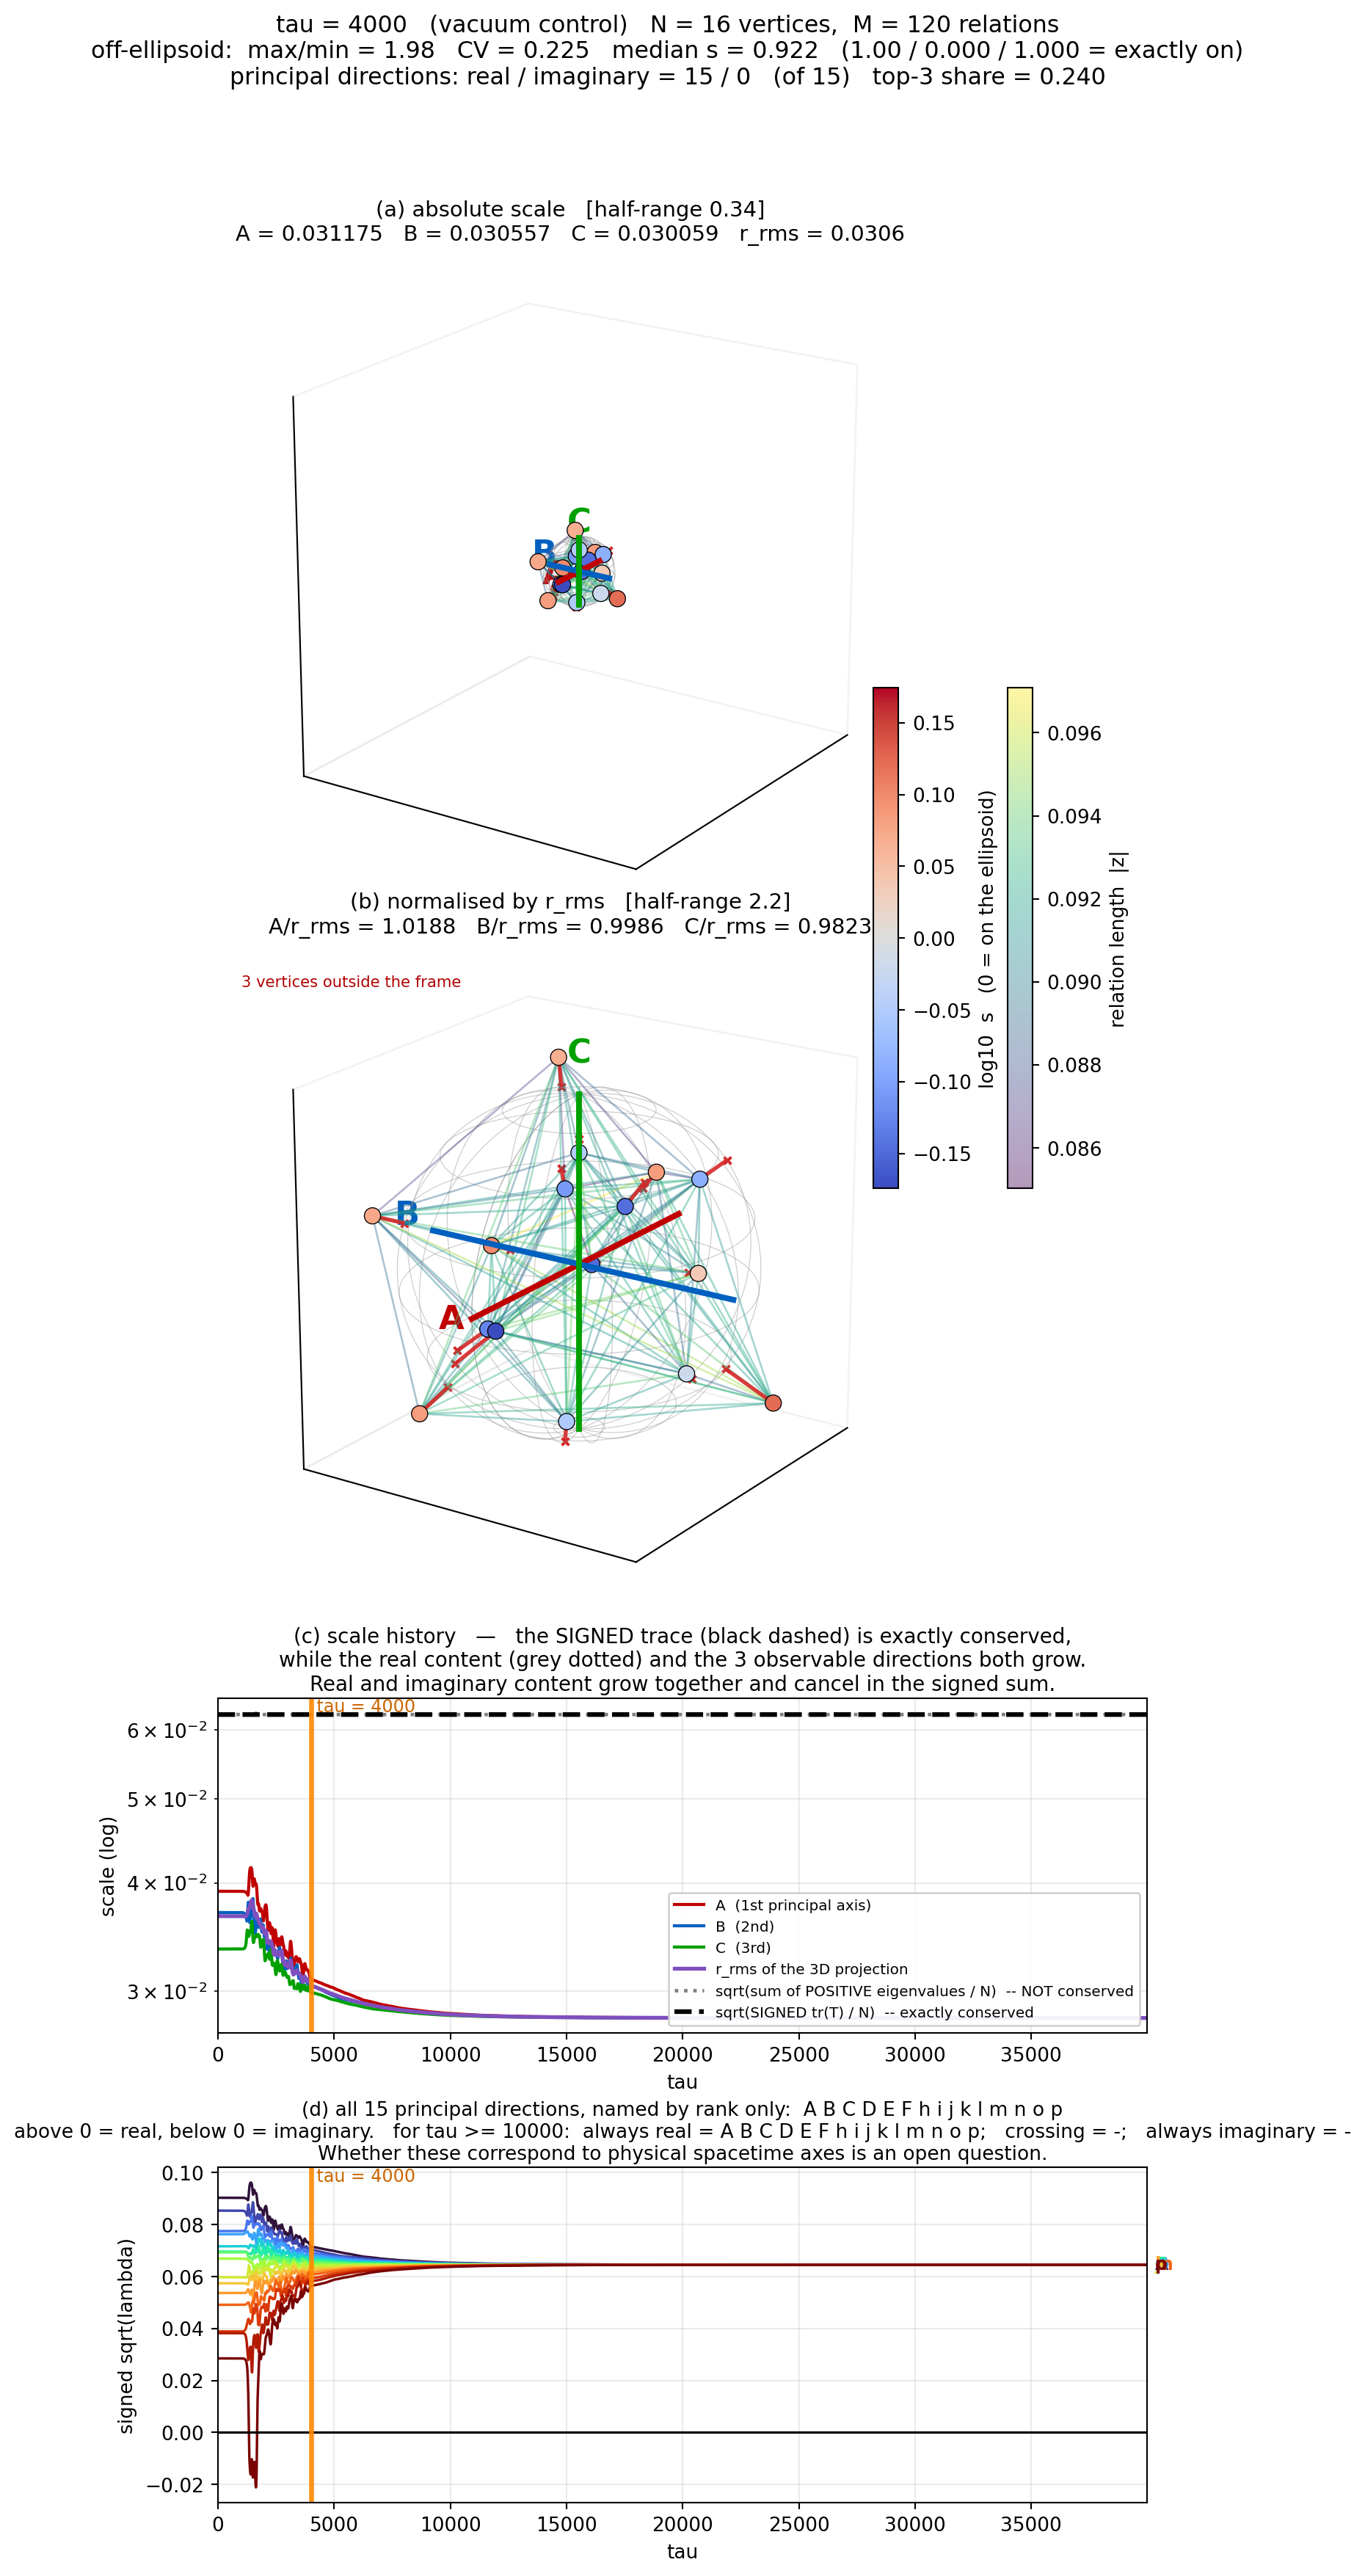
\includegraphics[keepaspectratio,alt={真空 τ=4000}]{複製_ダンプ版_v1/次元の生成構造/対照実験_N掃引1to20_三系_v2/figures_tau/fig_ellipsoid_tau04000_electron_T40000_d0.1_rep-dump40k16_N16_v_v1.png}} \\
9487 &
\pandocbounded{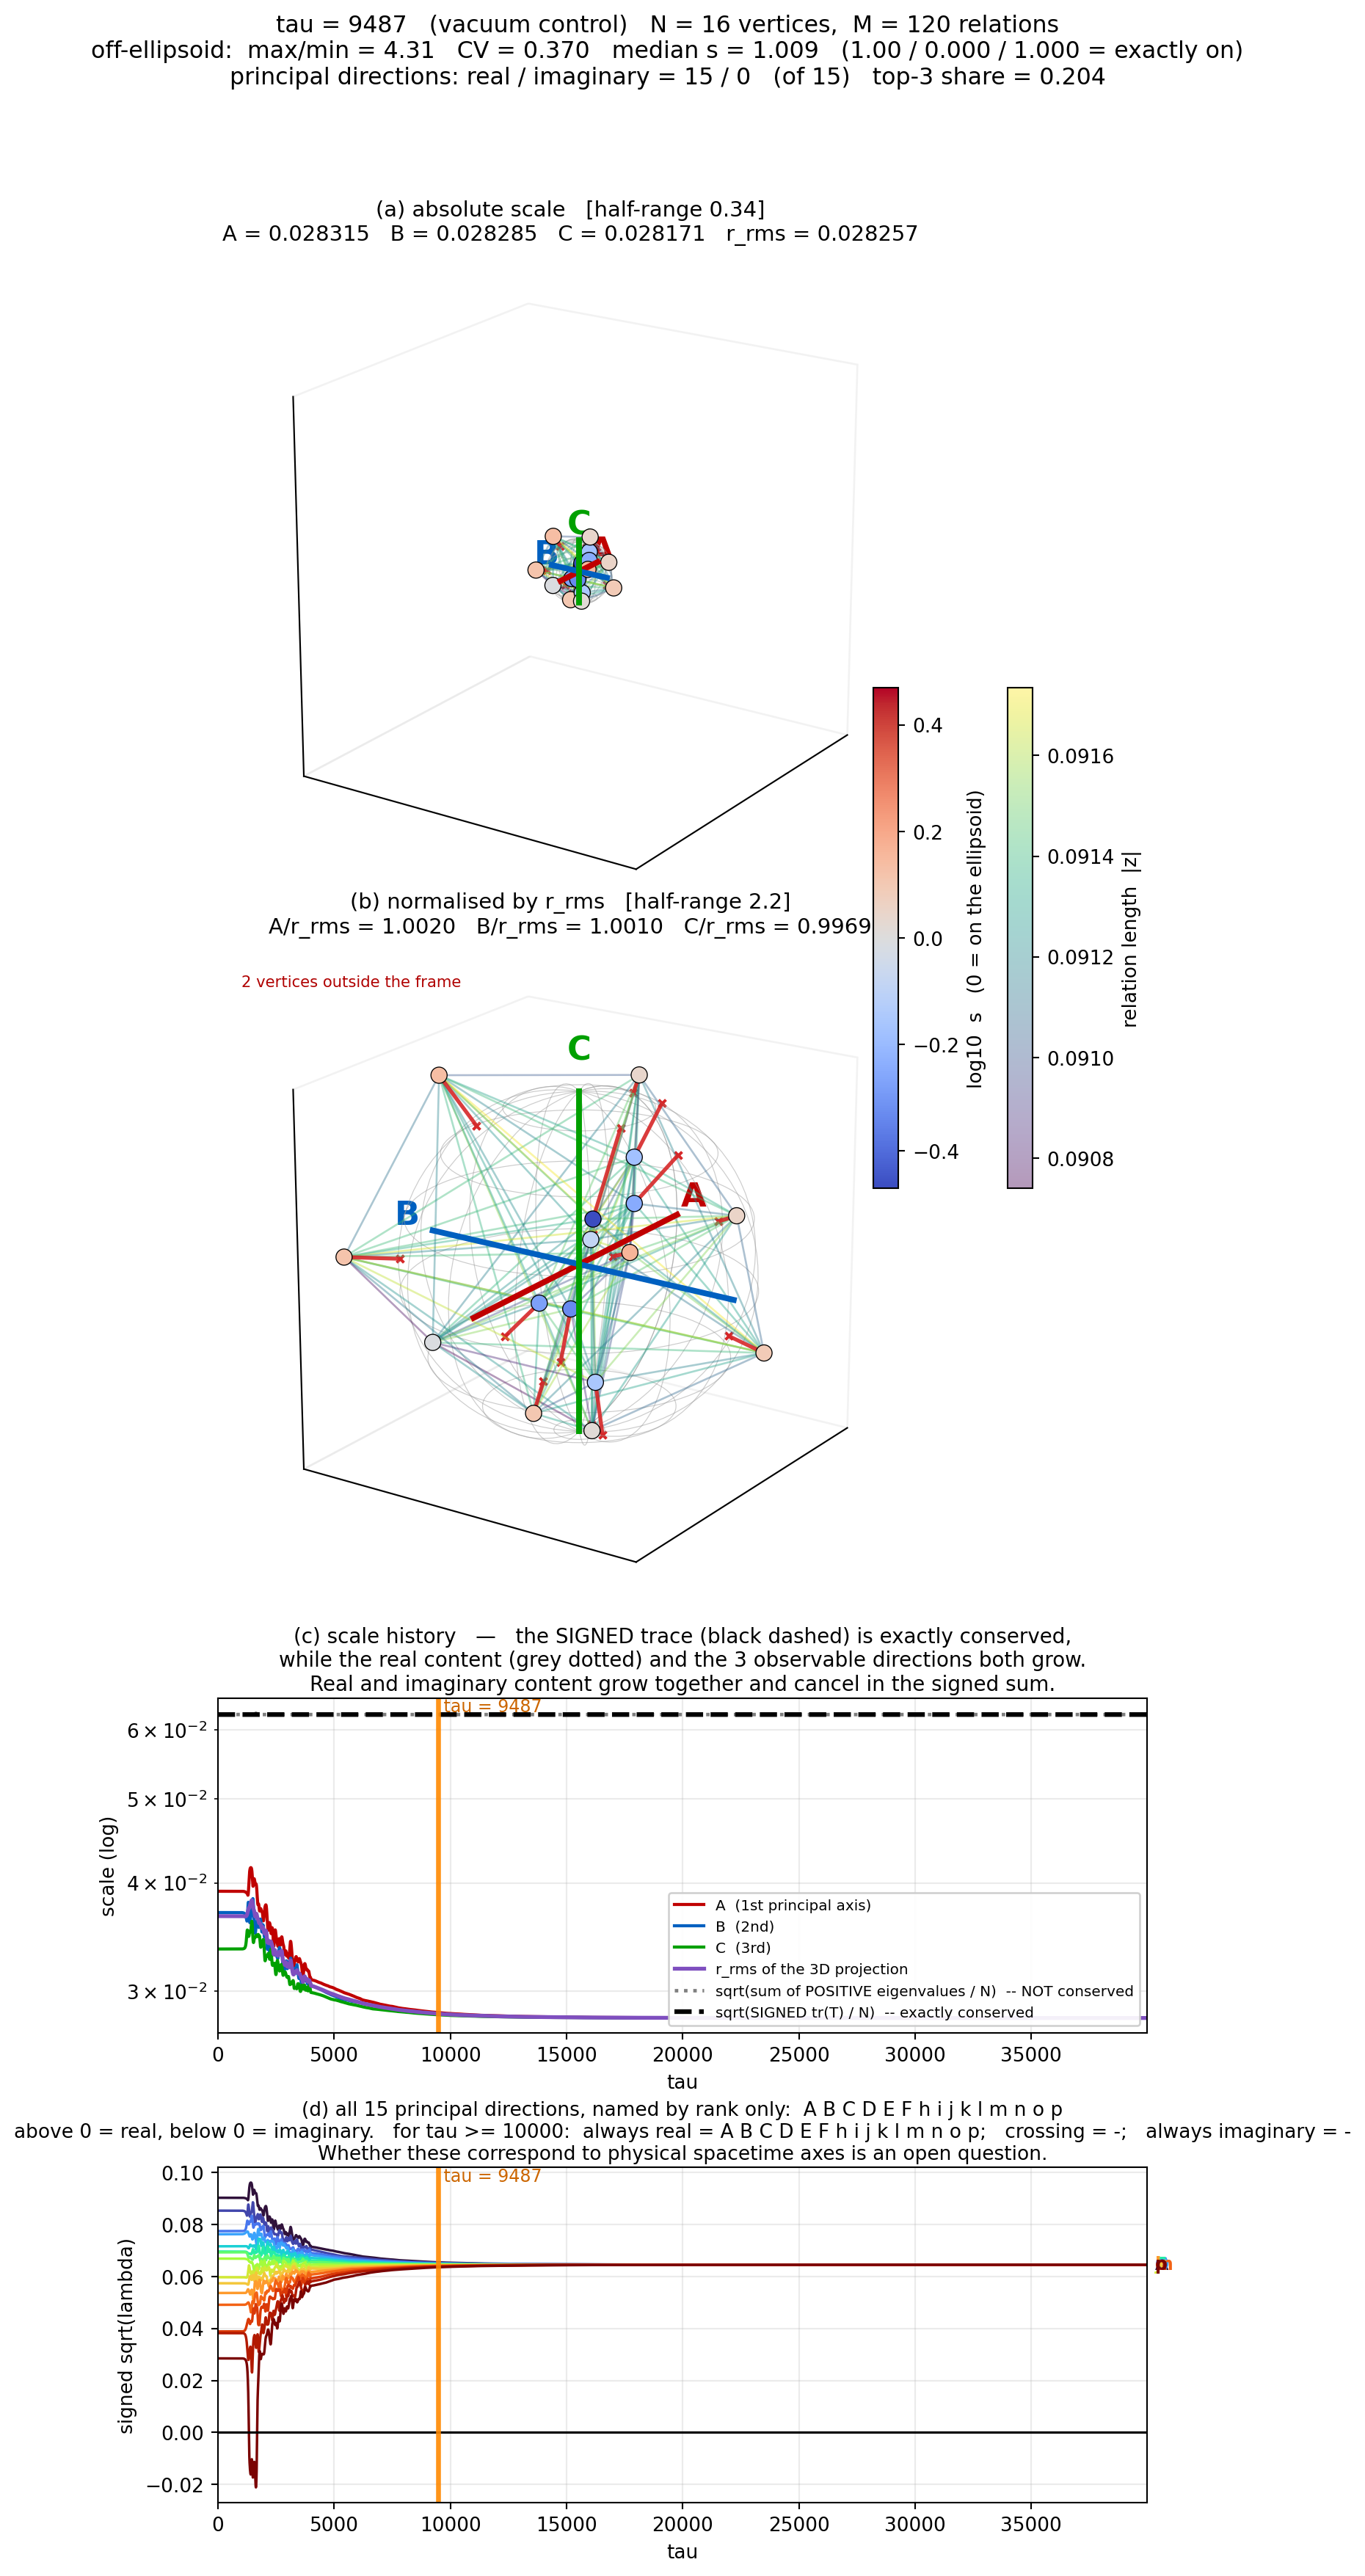
\includegraphics[keepaspectratio,alt={真空 τ=9487}]{複製_ダンプ版_v1/次元の生成構造/対照実験_N掃引1to20_三系_v2/figures_tau/fig_ellipsoid_tau09487_electron_T40000_d0.1_rep-dump40k16_N16_v_v1.png}} \\
39991 &
\pandocbounded{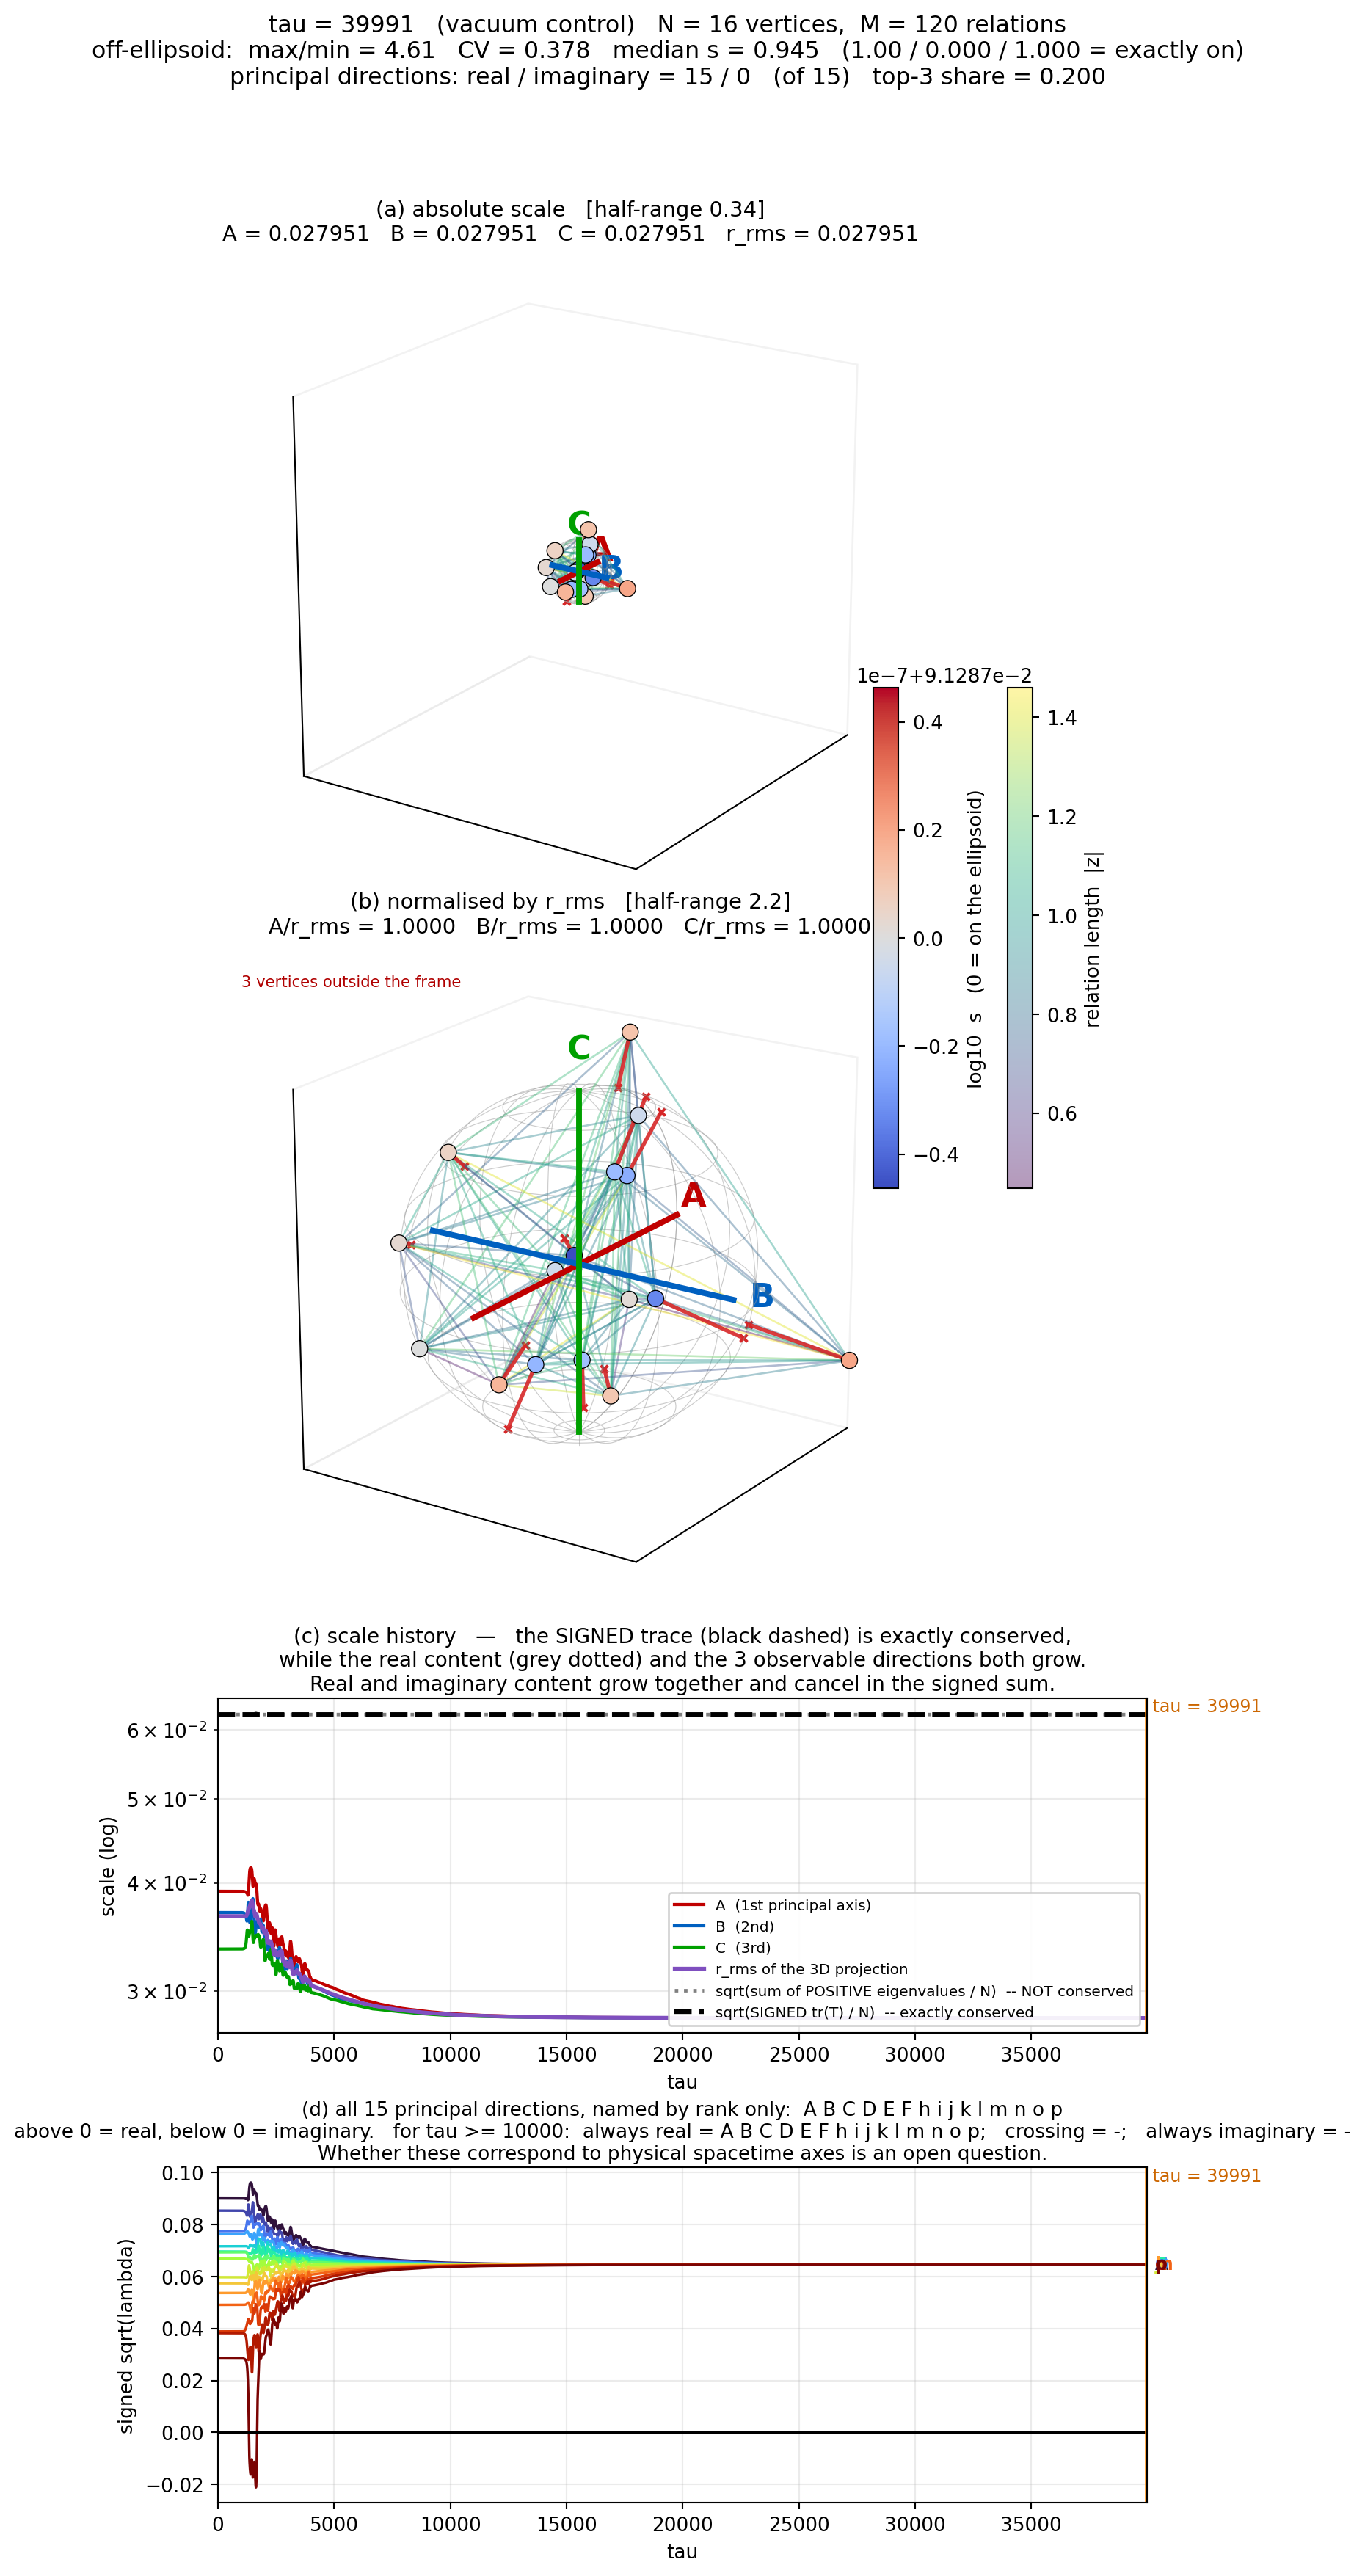
\includegraphics[keepaspectratio,alt={真空 τ=39991}]{複製_ダンプ版_v1/次元の生成構造/対照実験_N掃引1to20_三系_v2/figures_tau/fig_ellipsoid_tau39991_electron_T40000_d0.1_rep-dump40k16_N16_v_v1.png}} \\
\end{longtable}
}

\begin{center}\rule{0.5\linewidth}{0.5pt}\end{center}

\subsection{5.3 図の読み方 その1 ---
インフレーションの誤読を防ぐ}\label{ux56f3ux306eux8aadux307fux65b9-ux305dux306e1-ux30a4ux30f3ux30d5ux30ecux30fcux30b7ux30e7ux30f3ux306eux8aa4ux8aadux3092ux9632ux3050}

\textbf{この節は必読である。図5〜8
は二通りの正反対の誤読を招く。両方とも誤りである。}

\subsubsection{誤読1：「保存則が成り立っているのだから、拡大は起きていない」}\label{ux8aa4ux8aad1ux4fddux5b58ux5247ux304cux6210ux308aux7acbux3063ux3066ux3044ux308bux306eux3060ux304bux3089ux62e1ux5927ux306fux8d77ux304dux3066ux3044ux306aux3044}

\begin{enumerate}
\def\labelenumi{(\alph{enumi})}
\setcounter{enumi}{2}
\tightlist
\item
  段の\textbf{黒い破線}は \(\tau\)
  の全域で完全に水平である。これを見て「何も拡大していない」と読むのは誤りである。
\end{enumerate}

黒い破線が表しているのは\textbf{符号付き}トレース
\(\mathrm{tr}(B) = \sum_a \lambda_a\) である（\(B\)
は二重中心化グラム行列。慣性テンソル \(T\) ではない、主張5
の記号の注意）。ラグランジュの恒等式
\(\sum_{i<j}d_{ij}^2 = N\,\mathrm{tr}(B)\)
により、これは関係量のパワーそのものである。実測では後期968点の最小値と最大値が8桁まで一致する（相対幅
\(8.3\times10^{-9}\)）。\textbf{ただしこれは数値精度の範囲での保存であって、更新則から導いた解析的保存則ではない}（主張13
の分類）。

しかし\textbf{符号付き和が保存することは、各方向が動かないことを意味しない。}

同じ (c)
段の\textbf{灰色の点線}は正の固有値だけの和である。これは水平ではなく、転移で跳ね上がって
\(1.90\) 倍になる。絶対値和 \(\sum_a|\lambda_a|\) は \(2.79\)
倍になる。実方向の総量が増え、虚方向の総量がほぼゼロから現れ、その\textbf{差}が保存しているのである（主張13）。

指数関数的な増幅は実在する。(c) 段の赤・青・緑の線が
\(\tau \approx 9000\)
で垂直に跳ね上がっているのがそれである。\textbf{\(N=12\)
ではこの跳ね上がりが \(\tau \approx 2500\)
にあった。転移時刻は分解能に依存する。}

\subsubsection{\texorpdfstring{誤読2：「\(A\) が \(2.8\)
倍になったのだから、系全体が \(2.8\)
倍になった」}{誤読2：「A が 2.8 倍になったのだから、系全体が 2.8 倍になった」}}\label{ux8aa4ux8aad2a-ux304c-2.8-ux500dux306bux306aux3063ux305fux306eux3060ux304bux3089ux7cfbux5168ux4f53ux304c-2.8-ux500dux306bux306aux3063ux305f}

これも誤りである。符号付きトレースは動いていない。

観測される3方向が拡大するのは、次の\textbf{二つの効果の積}である。

\begin{enumerate}
\def\labelenumi{\arabic{enumi}.}
\tightlist
\item
  絶対値和が \(2.79\) 倍に増える
\item
  上位3方向の占有率が \(0.384\) から \(0.812\) へ上がる（集中）
\end{enumerate}

どちらか一方だけでは説明にならない。

\subsubsection{誤読3：「余剰次元がコンパクト化した」}\label{ux8aa4ux8aad3ux4f59ux5270ux6b21ux5143ux304cux30b3ux30f3ux30d1ux30afux30c8ux5316ux3057ux305f}

\textbf{これも誤りである。} \(m, n, o, p\)
は小さく丸まって観測から消えたのではない。

\begin{enumerate}
\def\labelenumi{(\alph{enumi})}
\setcounter{enumi}{3}
\tightlist
\item
  段を見ると、\(p\) は \(\tau \approx 9000\)
  でゼロを\textbf{通過して}下へ抜け、そのまま \(-0.19\)
  まで\textbf{絶対値を増やしながら}落ちていく。転移前後の比は \(5.568\)
  倍である。\(o\) も \(2.624\) 倍、\(n\) も \(1.674\) 倍、\(m\) も
  \(1.123\) 倍。\textbf{虚側へ移る4本はすべて絶対値を増やしている。}
  縮んでいるのは往復組の \(j\)（\(0.477\) 倍）と \(k\)（\(0.380\)
  倍）である。
\end{enumerate}

したがって起きているのは「余剰次元が縮んだ」ではなく、\textbf{「3方向が拡大し、7方向が符号を変えた（うち3本は往復）」}である。機構が違う。

\subsubsection{誤読4：「主軸が15本あるから、この系は15次元の平行多面体である」}\label{ux8aa4ux8aad4ux4e3bux8ef8ux304c15ux672cux3042ux308bux304bux3089ux3053ux306eux7cfbux306f15ux6b21ux5143ux306eux5e73ux884cux591aux9762ux4f53ux3067ux3042ux308b}

\textbf{これも誤りである。} 主軸の本数は
\(N-1 = 15\)、零閉鎖が要求する平行多面体の次元は \(d = 4\)（\(N = 2^4\)
より）であって、別物である（主張16-d）。系が平行多面体に到達したならランクは
\(4\) に落ちるはずだが、実測のランクは 8〜11 である。到達していない。

\subsubsection{図の見方の要点}\label{ux56f3ux306eux898bux65b9ux306eux8981ux70b9}

\begin{itemize}
\tightlist
\item
  \begin{enumerate}
  \def\labelenumi{(\alph{enumi})}
  \tightlist
  \item
    段は全 \(\tau\) で枠が \(\pm 0.17\) に固定してある。\(\tau = 4000\)
    の図と \(\tau = 39991\)
    の図を並べると、楕円体そのものが枠に対して大きくなっているのが直接見える。
  \end{enumerate}
\item
  \begin{enumerate}
  \def\labelenumi{(\alph{enumi})}
  \setcounter{enumi}{1}
  \tightlist
  \item
    段は \(r_{\rm rms}\)
    で割ってあるので、大きさの情報が消えて形だけが残る。\(\tau = 39991\)
    で \(A/r_{\rm rms} = 1.230\)、\(C/r_{\rm rms} = 0.529\)
    と、扁平になっているのがわかる。
  \end{enumerate}
\item
  \begin{enumerate}
  \def\labelenumi{(\alph{enumi})}
  \setcounter{enumi}{2}
  \tightlist
  \item
    段の縦線が現在の \(\tau\) である。各図がどの時点かを (c)
    段の中で確認できる。\textbf{(a)
    段の絶対スケールだけを見て時系列を判断してはならない。}
  \end{enumerate}
\item
  \begin{enumerate}
  \def\labelenumi{(\alph{enumi})}
  \setcounter{enumi}{3}
  \tightlist
  \item
    段の右端の文字が15本の主軸の名前である。
  \end{enumerate}
\end{itemize}

\subsubsection{真空対照との比較}\label{ux771fux7a7aux5bfeux7167ux3068ux306eux6bd4ux8f03}

図9〜12（真空）では、(c)
段の黒破線も灰点線も\textbf{両方とも}水平である。転移が起きないので絶対値和も増えない。(d)
段の15本は全て正の側に留まり、\(\tau = 39991\) では全て \(0.0645\)
に集まって完全等方になる。

\textbf{図5〜8
で見えている拡大と虚方向への転落は、いずれも物質の生成に伴う現象であって、系が最初から持っていた性質ではない。}
これが対照実験の結論である。

\begin{center}\rule{0.5\linewidth}{0.5pt}\end{center}

\subsection{\texorpdfstring{5.4 図の読み方 その2 ---
\(A,B,C,D,E,F,h,i,j,k,l,m,n,o,p\)
の15本の主軸とは何か}{5.4 図の読み方 その2 --- A,B,C,D,E,F,h,i,j,k,l,m,n,o,p の15本の主軸とは何か}}\label{ux56f3ux306eux8aadux307fux65b9-ux305dux306e2-abcdefhijklmnop-ux306e15ux672cux306eux4e3bux8ef8ux3068ux306fux4f55ux304b}

\subsubsection{なぜ15本なのか}\label{ux306aux305c15ux672cux306aux306eux304b}

分解能 \(N = 16\) の系は \(M = N(N-1)/2 = 120\)
本の関係を持つ。各関係量から長さ \(d_{ij}\) を読み、二重中心化

\[B = -\tfrac12\,J\,D^{\circ 2}\,J,\qquad J = I - \tfrac1N\mathbf{1}\mathbf{1}^{\mathsf T}\]

によりグラム行列を作ると、\(B\mathbf{1} = 0\)
が厳密に成り立つ。この自明ゼロは主軸ではないから、主軸は \(N - 1 = 15\)
本である。

\textbf{15 という数は分解能 \(N=16\) から出た \(N-1\)
であって、外から選んだ数ではない。} \(N\) を変えれば \(N-1\)
に変わる（\(N=12\) なら 11 本だった）。この点で、超弦理論の \(10\) や
\(11\) のように理論の無矛盾性から一意に決まる次元数とは性格が異なる。

\textbf{そして \(N\) の選び方には根拠がある。}
平行多面体族として零閉鎖を実現するなら \(N = 2^d\)
であり（主張16）、本ノートは \(N = 16 = 2^4\)
を採る。したがって主軸の本数は \(2^d - 1 = 15\) である。\(d\) と
\(2^d-1\) を混同しないこと（主張16-d）。

\subsubsection{15本が何をしているか}\label{ux672cux304cux4f55ux3092ux3057ux3066ux3044ux308bux304b}

{\def\LTcaptype{none} % do not increment counter
\begin{longtable}[]{@{}
  >{\raggedright\arraybackslash}p{(\linewidth - 8\tabcolsep) * \real{0.2000}}
  >{\raggedright\arraybackslash}p{(\linewidth - 8\tabcolsep) * \real{0.2000}}
  >{\raggedright\arraybackslash}p{(\linewidth - 8\tabcolsep) * \real{0.2000}}
  >{\raggedright\arraybackslash}p{(\linewidth - 8\tabcolsep) * \real{0.2000}}
  >{\raggedright\arraybackslash}p{(\linewidth - 8\tabcolsep) * \real{0.2000}}@{}}
\toprule\noalign{}
\begin{minipage}[b]{\linewidth}\raggedright
組
\end{minipage} & \begin{minipage}[b]{\linewidth}\raggedright
主軸
\end{minipage} & \begin{minipage}[b]{\linewidth}\raggedright
転移前後の比
\end{minipage} & \begin{minipage}[b]{\linewidth}\raggedright
実／虚
\end{minipage} & \begin{minipage}[b]{\linewidth}\raggedright
役割
\end{minipage} \\
\midrule\noalign{}
\endhead
\bottomrule\noalign{}
\endlastfoot
\textbf{\(A, B, C\)} & 第1〜3 & \(2.80\) / \(1.73\) / \(1.42\) & 実 &
\textbf{拡大する。3次元射影に現れる。図化に使う} \\
\textbf{\(D, E, F, h, i\)} & 第4〜8 & \(1.27\) / \(1.14\) / \(1.01\) /
\(0.87\) / \(0.71\) & 実 &
\textbf{ほぼ変わらない。実軸だが射影には現れない} \\
\textbf{\(j, k, l\)} & 第9〜11 & \(0.48\) / \(0.38\) / \(0.73\) & 往復 &
\textbf{実虚の境界を行き来する。虚方向の本数が4〜7で揺れる原因} \\
\textbf{\(m, n, o, p\)} & 第12〜15 & \(1.12\) / \(1.67\) / \(2.62\) /
\(5.57\) & 虚 & \textbf{虚側に落ちる。ただし絶対値は増える} \\
\end{longtable}
}

実軸は \(A\)〜\(i\) の8本、虚軸は \(m,n,o,p\)
の4本で確定しており、\(j,k,l\)
の3本が境界を往復する。「虚6本」が最も多い（968点中616点）。

\subsubsection{名前が序数であることの意味}\label{ux540dux524dux304cux5e8fux6570ux3067ux3042ux308bux3053ux3068ux306eux610fux5473}

\(A\) から \(p\)
までの名前は、\textbf{その時刻における固有値の大小順}を表すだけである。次のことに注意しなければならない。

\begin{enumerate}
\def\labelenumi{\arabic{enumi}.}
\tightlist
\item
  \textbf{名前は物理量ではない。} \(A\) が「時間軸」であるとか \(B\)
  が「\(R\)」であるといった対応は、一切主張していない。
\item
  \textbf{同じ名前が同じ方向を指し続けるとは限らない。}
  固有値が縮退する時刻では順序が入れ替わる。\(N=16\)
  の実測最小ギャップは \(3.4\times10^{-6}\)〜\(5.1\times10^{-5}\)
  であり、\(N=12\) より一桁小さい。縮退は現実に起きている。
\item
  \textbf{主軸ベクトルは時間的に連続しない。}
  第1主軸ベクトルの内積の絶対値は \(\tau = 4000\) と \(\tau = 39991\)
  の間でわずか \(0.0450\)、\(\tau = 9487\) と \(\tau = 39991\) の間では
  \(0.0233\) である。つまり転移直後の \(A\) と終了時の \(A\)
  は、ほとんど直交した別の方向である。
\end{enumerate}

\textbf{したがって (d)
段の15本の線は「15個の物理的な軸の時間発展」ではない。「各時刻において固有値の大きさで順位付けした値の系列」である。}
この区別は重要である。

\subsubsection{物理への同定は今後の課題である}\label{ux7269ux7406ux3078ux306eux540cux5b9aux306fux4ecaux5f8cux306eux8ab2ux984cux3067ux3042ux308b}

15方向のうち3方向が急拡大し、5方向がほぼ不変にとどまり、7方向が虚方向へ移る（うち3本は往復）という構造が得られた。しかし、

\begin{quote}
\textbf{これらが物理的時空（時間1軸＋空間3軸、あるいは \(R\) と
\(Q\)）に同定できるのか、同定できないのか、あるいは別の写像を挟む必要があるのかは、今後の課題である。同定できる根拠は現時点で何もない。}
\end{quote}

同様に、

\begin{quote}
\textbf{この15本の主軸からなるスペクトル構造が超弦理論をはじめとする既存の高次元理論とどのような関係にあるのかも、今後の課題である。}
\end{quote}

\textbf{v3 まで本ノートは \(N=12\) を採っていたため主軸が 11
本であり、超弦理論の 11
次元と数が一致していた。これは分解能の選び方による偶然である。} \(N=16\)
では 15 本になる。§5.3 の誤読3
で述べた通り機構も異なる（コンパクト化ではない）。また出所も異なる（本模型では
\(N-1\)、超弦理論では無矛盾性）。\textbf{語の一致をもって理論の対応を主張しない。}

\begin{center}\rule{0.5\linewidth}{0.5pt}\end{center}

\subsection{5.5 図13 ---
準振動とその周期（主張15）}\label{ux56f313-ux6e96ux632fux52d5ux3068ux305dux306eux5468ux671fux4e3bux5f3515}

\begin{figure}
\centering
\pandocbounded{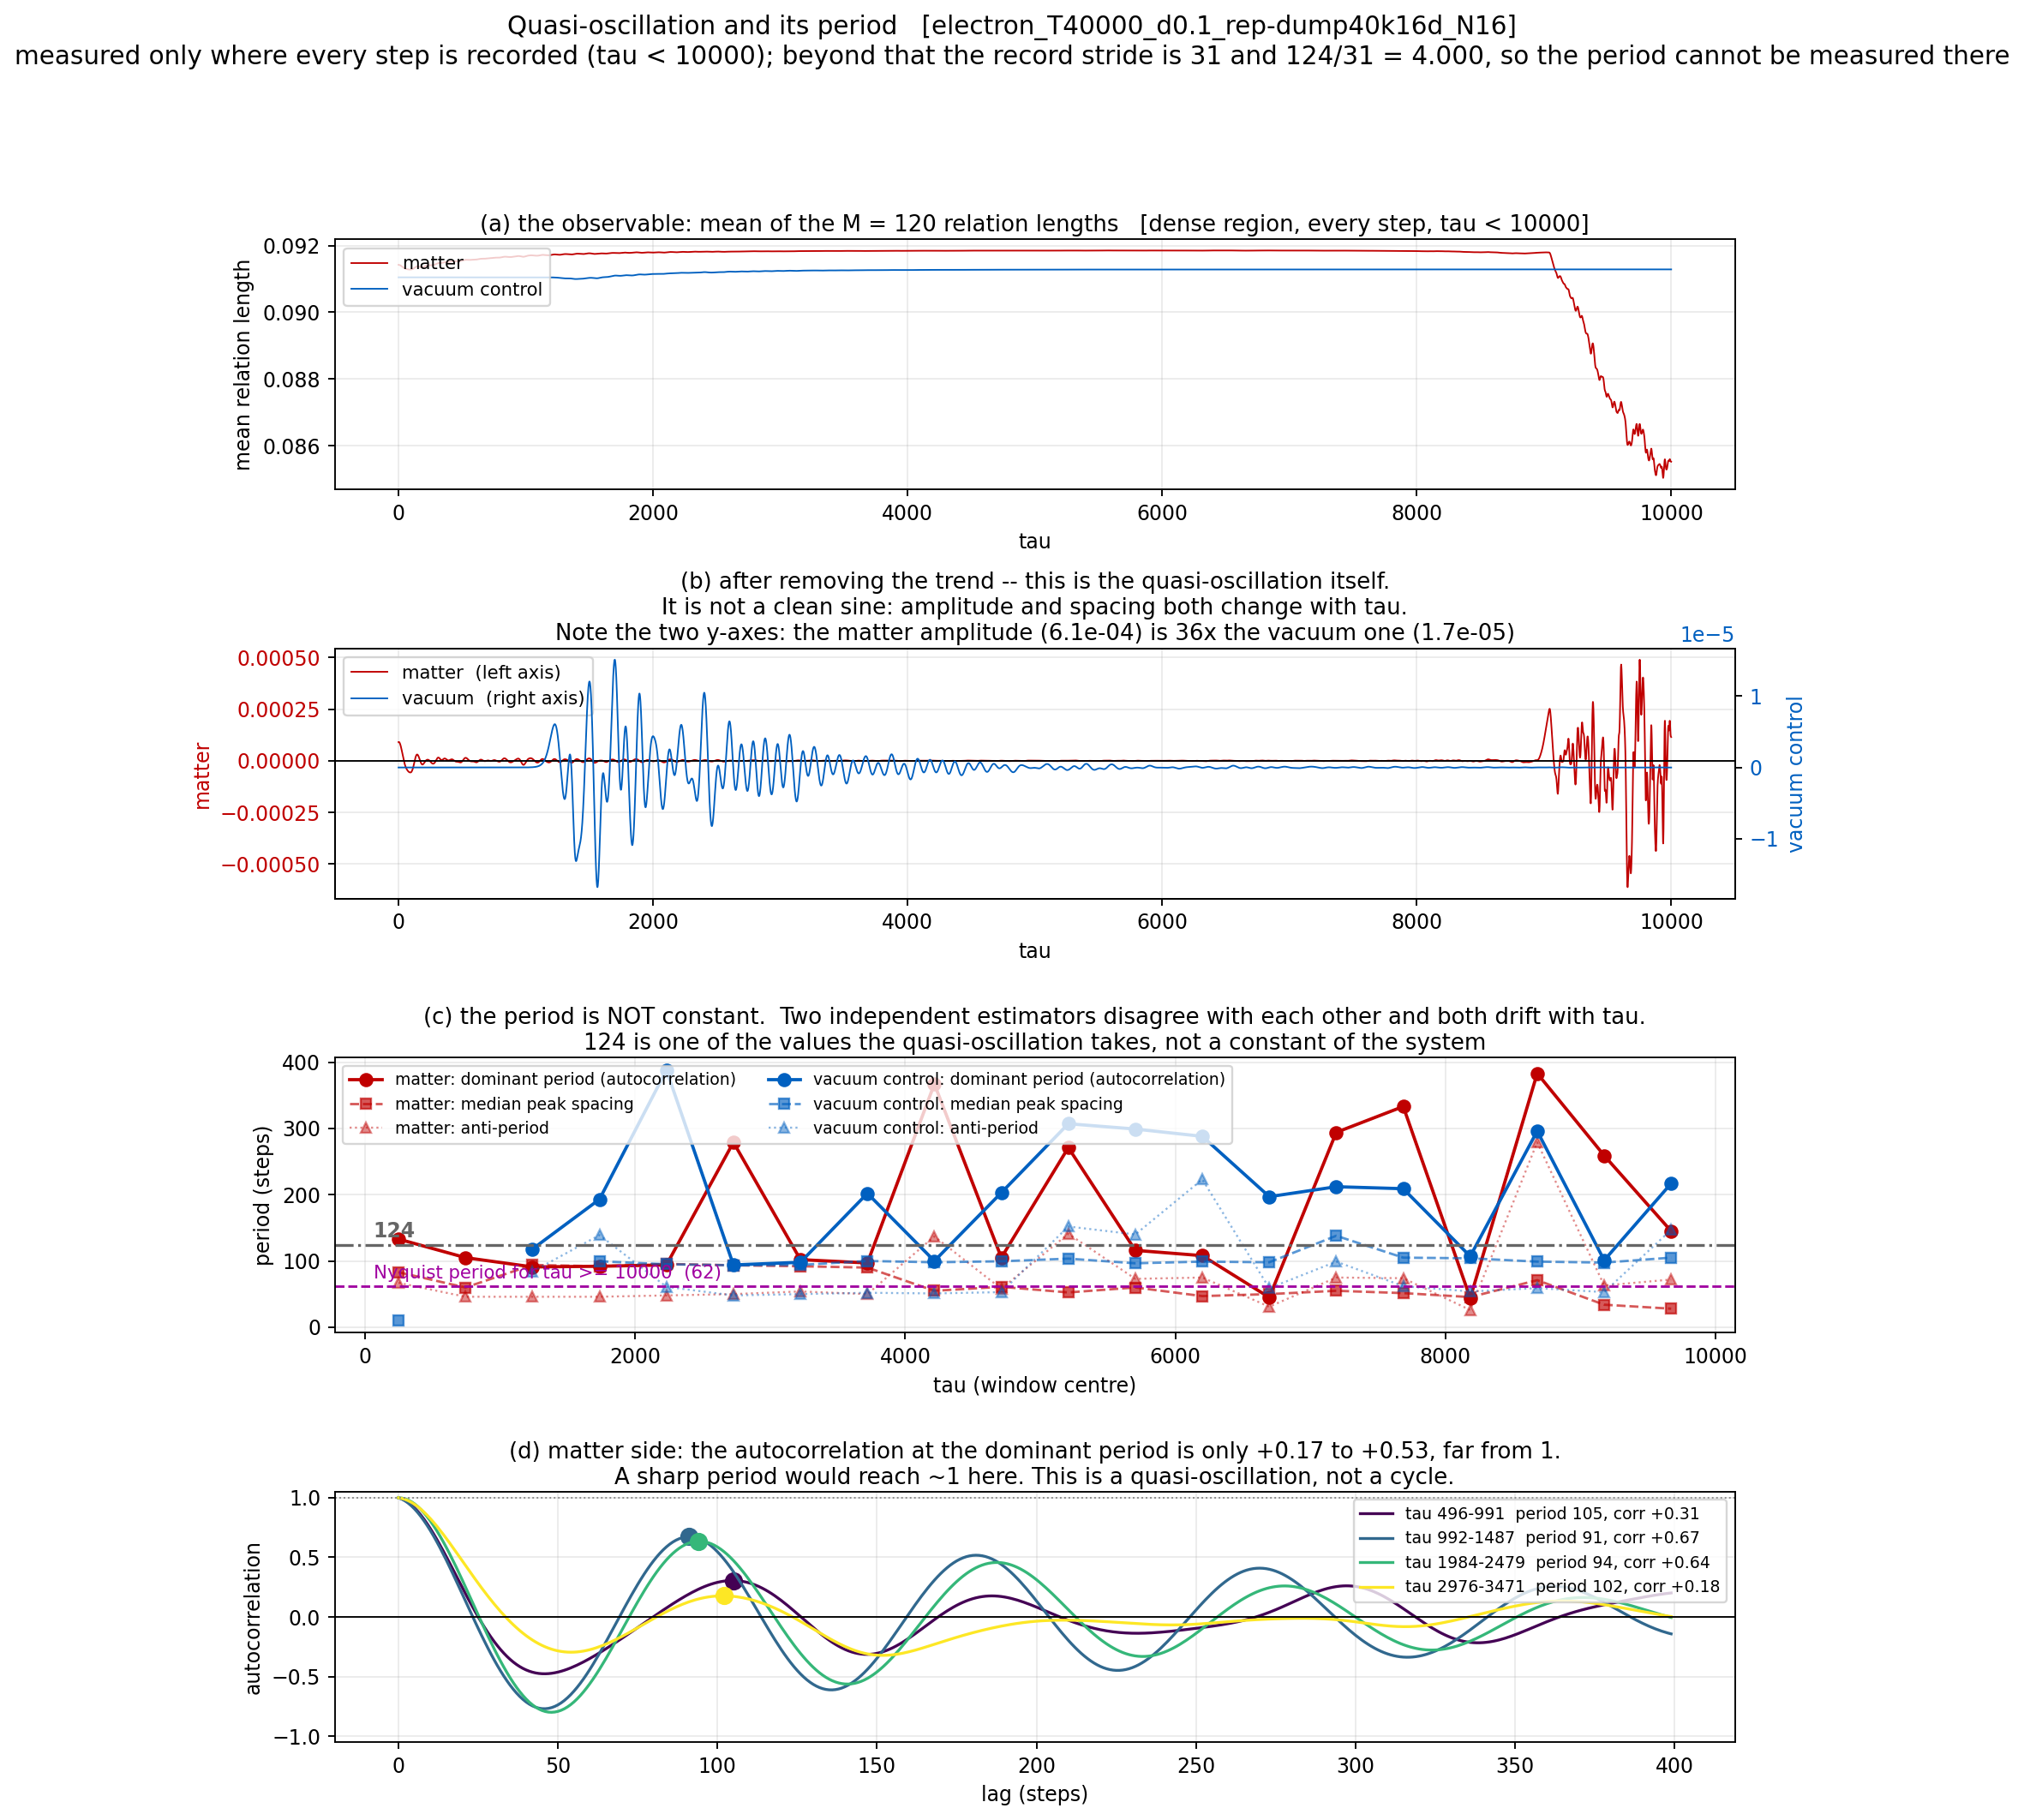
\includegraphics[keepaspectratio,alt={図13}]{複製_ダンプ版_v1/次元の生成構造/対照実験_N掃引1to20_三系_v2/figures_tau/fig_period_electron_T40000_d0.1_rep-dump40k16d_N16_v1.png}}
\caption{図13}
\end{figure}

導出プログラムは
\texttt{複製\_ダンプ版\_v1/次元の生成構造/対照実験\_N掃引1to20\_三系\_v2/make\_period\_figure\_v1.py}。測定値そのものは
\texttt{複製\_ダンプ版\_v1/次元の生成構造/対照実験\_N掃引1to20\_三系\_v2/figures\_tau/period\_series\_electron\_T40000\_d0.1\_rep-dump40k16d\_N16\_v1.npz}
に保存してある。

\textbf{この図は密領域を \(\tau<10000\)
に広げた専用走行（\texttt{...rep-dump40k16d\_N16}）によるもので、転移（\(\tau\approx9000\)）を含む。}
楕円体図（図5〜12）の走行 \texttt{...rep-dump40k16\_N16}
とは同一条件・同一乱数で、密領域の取り方だけが異なる。

{\def\LTcaptype{none} % do not increment counter
\begin{longtable}[]{@{}
  >{\raggedright\arraybackslash}p{(\linewidth - 2\tabcolsep) * \real{0.5000}}
  >{\raggedright\arraybackslash}p{(\linewidth - 2\tabcolsep) * \real{0.5000}}@{}}
\toprule\noalign{}
\begin{minipage}[b]{\linewidth}\raggedright
段
\end{minipage} & \begin{minipage}[b]{\linewidth}\raggedright
内容
\end{minipage} \\
\midrule\noalign{}
\endhead
\bottomrule\noalign{}
\endlastfoot
(a) &
観測量そのもの。120本の関係長の平均。密領域（全ステップ記録）のみ \\
(b) & 201点移動平均を引いた残り。これが準振動そのもの \\
(c) & 卓越周期の \(\tau\)
依存。自己相関法（丸・実線）と山間隔法（四角・破線）と反周期（三角・点線）を重ねた \\
(d) & 自己相関そのもの。物質側の4窓 \\
\end{longtable}
}

\textbf{この図の読み方}

\begin{itemize}
\tightlist
\item
  (a)：物質側（赤）は \(\tau \approx 8900\)
  まで平坦で、そこから\textbf{急落する}。これが転移である。真空側（青）は全区間で平坦のままである。\(N=12\)
  では同じ急落が \(\tau \approx 2300\) にあった。
\item
  (b)：\textbf{左右で軸が違う。}
  物質側（左軸）は転移まで振幅がほぼ零で、\(\tau \approx 8900\)
  から一気に立ち上がる。真空側（右軸、\(10^{-5}\) 台）は
  \(\tau \approx 1200\)〜\(4000\)
  に一度きれいな振動を見せてから減衰する。\textbf{転移前には物質側の振動がむしろ真空側より小さい区間がある}（\(\tau\in[3968,8927]\)、主張15
  の項目7）。この区間の山間隔をノイズと判定した根拠がこの段である。
\item
  (c)：\textbf{この段が主張15 の核心である。} 灰色の一点鎖線が \(124\)
  である。2本の推定線はどちらもこの線の上を横切るだけで、その上に留まらない。\textbf{2つの推定法が互いに一致しないこと、そしてどちらも
  \(\tau\)
  とともに漂動することが、単一の鋭い周期が存在しないことの証拠である。}
  紫の破線は \(\tau \ge 10000\) におけるナイキスト周期 \(62\)
  で、この線より下は後期には測れない領域である。\textbf{転移後の山間隔
  \(34.0 \to 28.0\)
  はこの線より下にある}から、粗い記録の走行では原理的に捉えられなかった。
\item
  (d)：\textbf{鋭い周期であれば、卓越周期のラグで自己相関が \(1\)
  に達するはずである。} \(N=16\) の実測は \(+0.134\)〜\(+0.673\)
  にとどまる（各曲線上の丸印）。これが「巡回」ではなく「準振動」だと判断した根拠である。曲線の形も窓ごとに違う。
\end{itemize}

\textbf{この図が禁じる誤読}

\begin{quote}
「\(124\) ステップの周期がある」------正確ではない。\(124\)
は準振動が取る値の一つであって、系の定数ではない。(c) 段の2本の推定線が
\(124\) の線上に載っていないことを見ること。

「周期があるから \(U^n = I\)
が確認された」------確認されていない。\(U^n = I\) に由来するなら周期は
\(n\) で決まる定数のはずである。実測は変動している。\(U^n = I\)
によるものか別の現象かは未決着である。
\end{quote}

\begin{center}\rule{0.5\linewidth}{0.5pt}\end{center}

\subsection{6.
本ノートが確定させたこと}\label{ux672cux30ceux30fcux30c8ux304cux78baux5b9aux3055ux305bux305fux3053ux3068}

冒頭に挙げた二つの問いへの答えは以下である。

\textbf{問1：波を複素数で表現することは必須か。}

必須ではない（主張9）。複素数が実の符号不定形に対して追加しているのは
\(\sum q_np_n = 0\)
一本だけである（主張8）。\textbf{ただしこれを「スケール対称性の言い換え」と呼んではならない。}
それは主張8 で撤回した生成子の議論に戻ることになる。

\textbf{したがって複素表現は必須ではない。}
ただし\textbf{「公理を一つ節約する便法」という言い方は正確でない}。第0.5公理の読み
A
を独立公理から外せる理由は\textbf{零閉鎖式の同次性}であって、複素表現そのものではない（同次式なら複素かどうかに依らず解集合は錐である）。\textbf{複素表現が実の符号不定形に追加しているのは直交条件
\(\sum q_np_n = 0\) である。}

\textbf{問2：複素表現した場合の中心投影はどういう形になるか。}

中心投影の中心は頂点ではなく、主観空間から観測できない。虚数記号が付くのは中心方向だけであり、線分の長さは全て実数のままである（主張7）。

\textbf{そして中心投影の定式化では仮定（S）が成立するため（主張7）、「多体問題が一本のスカラー等値拘束へ縮約される」構造が保たれる（主張0）。}
実数では \(\sum x_n^2 = R^2\) が半径 \(R\) の球殻表面上の任意の点 \(P\)
を表し、拘束は \(X^{\mathsf T}F(X) = 0\) の一本に縮約された。複素では

\[x^2 + y^2 + z^2 - t^2 = R^2 + Q^2\]

となる。これは4変数のままでは符号数 \((3,1)\)
の一葉双曲面であって閉じない。\textbf{保存量 \(C = t^2+R^2+Q^2\)
を固定し、さらに仮定（U：状態が3次元部分空間に載る）と（R：読出しが線形正則
\(X = \Lambda u\)）を置けば、\(G = (\Lambda^{-1})^{\mathsf T}\Lambda^{-1}\)
の定める閉曲面（楕円面）になる}（主張0-c）。\textbf{\(t\)
だけを固定しても \(R, Q\) が動けば \(C\)
は変わるので、一枚の閉曲面にはならない。}

\textbf{縮約そのものは（S）だけで成立し、（U）（R）を要しない。}
（U）（R）は観測座標との対応をつけるために要る。

\textbf{ただし二点を混同してはならない。}
第一に、保存量は運動を決めるのではなく、\textbf{許される運動の空間を決める}だけである。第二に、この楕円面が\textbf{慣性楕円体そのものであることは未証明である}。それには
\(G^{-1}\propto T\) を示す必要があり、読出し写像 \(\Lambda\)
が未与である以上（主張2B）、現時点では示せない。\textbf{これが本ノートにおける最大の未導出部分である。}

\textbf{ただし右辺が保存するために必要なのは \(\dot C=0\)
であり、本模型の成分層でそれが期待できるのは定常解である。}
過渡期および準安定状態では逸脱し、振動する場合もある（主張0-d、主張10、主張15）。層の区別も要る。上の逸脱は成分の層での話であり、読出しの層には転移を貫通して保存する量が存在する（主張18-c・18-d）。

この形の零閉鎖を満たす配置として\textbf{平行多面体}が存在する（主張4-b、全
\(d\) で成立）。その場合の頂点数は \(N = 2^d\)
である。\textbf{ただし零閉鎖する配置が平行多面体に限られることは
\(d\ge3\)
で未証明である}（主張4-e）。中心対称かつ凸では足りないことは反例で示した（4-d）。平行多面体は必ず楕円体に内接し、その外接楕円体は\textbf{正規化慣性楕円体（\(c = d/N\)）}と一致する（主張6B）。そして配置の二次の情報は慣性楕円体に尽き、多重極
\(l\le2\) で飽和する（主張6）。

すなわち\textbf{中心投影と零閉鎖を同時に満たす、厳密に構成可能な一族}として、\textbf{\(d\)
本の線分のミンコフスキー和として作られ、一つの楕円体に内接し、その楕円体の情報が
\(l\le2\)
で飽和する配置}がある。\textbf{これが唯一の一族であるかは未証明である}（主張4-e）。

\textbf{v3 で追加した問3：数値模型は実際にその配置になっているか。}

なっていない。

\begin{itemize}
\tightlist
\item
  \textbf{成分の層では}、零閉鎖は定常状態でのみ成立する恒等式であり、過渡状態と準安定状態では破れる。楕円面からの偏差は
  \(\tau\) とともに単調に減らず、転移後 36,000 ステップにわたり max/min
  \(= 12\) 前後に留まる（主張10）
\item
  この偏差はシード強度に依存する。本走行の \(\delta = 0.1\)
  は大きい。\textbf{シードを弱めた場合・\(\tau\)
  を伸ばした場合に偏差が漸減するかは未確認である}（主張11）
\item
  配置は平行多面体に到達しない。ランクは \(15\) から \(8\)〜\(11\)
  へ落ちるが \(d = 4\) までは落ちない（§3B）
\item
  系の二重中心化読出しは \(N-1 = 15\) 本の非自明な主軸を持ち、上位3方向
  \(A,B,C\) へのスペクトル集中により観測スケールが拡大する。\(D\)〜\(i\)
  はほぼ不変、\(m,n,o,p\) は虚方向へ移り、\(j,k,l\)
  は往復する。\textbf{これが「余剰方向が小さく縮んで見えなくなる」型のコンパクト化でないこと}は確定したが、\textbf{物理的時空への同定は今後の課題であり、根拠は何もない}（主張12）
\item
  平行多面体族として零閉鎖を実現する場合、分解能は \(N = 2^d\)
  になる。本ノートは
  \(N=16\)（\(d=4\)）を採る。ただしこれは十分条件ではなく（rank \(= d\)
  も単独では足りない）、全零閉鎖解に対する必要条件であることも未導出である（主張16）
\item
  平行多面体を選び出しているのは \(\sum x_n^2 = 0\)
  という式の形ではなく、面次元による符号則である。符号と配置をともに自由に選べるなら
  \(N \ge 3\) で非自明解が存在してしまう（主張17）
\item
  保存するのは符号付きトレースであり、実方向の総量と虚方向の総量はともに増えて相殺する（主張13）
\item
  虚方向は真空には存在せず、物質の生成とともに現れる（主張14）
\item
  主軸の\textbf{向きは保存しない}。上位3主軸の部分空間は約 2000
  ステップで乱数基準まで相関を失い、\(36{,}000\)
  ステップ掃引しても安定化しない。しかし\textbf{向きに依らない保存量（二次形式）は存在する}。\(\sum_e\lvert x_e\rvert^2\)
  と \(\sum_e x_e^2\)
  の少なくとも2種類が確認され、どちらもトレース型なので向きの拡散の影響を受けない。とくに
  \(\sum_e x_e^2\)
  は\textbf{複素数として転移を貫通して不変}である（主張18）
\item
  \(10^2\) ステップ規模の準振動が存在するが、周期は \(\tau\)
  とともに変動する。\(N=16\) では転移前の山間隔 \(90\)〜\(95.5\)
  が転移域で \(34.0\)、転移直後で \(28.0\) へ短縮し、真空側は
  \(93.5\)〜\(138\) のまま短縮しない。\textbf{転移が周期を短くするという
  \(N=12\) の所見は \(N=16\) でも再現した。} ただし\textbf{これが第2公理
  \(U^n = I\) によるものか別の現象かは今後の課題である}（主張15）
\end{itemize}

\textbf{v4 で追加した問4：表題の「4次元」とは何か。}

\((r, t, R, Q)\)
を座標とする\textbf{4次元}である（主張2B）。そして零閉鎖が

\[r^2 = t^2 + R^2 + Q^2\]

を与えるので、この4次元空間の中に\textbf{光錐型の零錐}がある。\textbf{これが表題の意味である。}

\(x, y, z\)
はその後の3次元読出しの話であり、4次元という主張には要らない。関係性が与えるのは長さ
\(r\) だけで、\(x,y,z\) は \(r\) が許す面 \(S_r^2\)
の上の点である（主張2B）。零錐上の自由度は 3、射影化すれば 2 である。

\textbf{平行多面体の次元
\(d = 4\)（\(N=16\)、主張16）とは別物である。数字の一致は偶然であって、一方から他方は導かれない。}

\textbf{v4 で追加した問5：向きは安定するのか。}

しない（主張18-a）。しかし\textbf{重要なのは向きではなく、向きに依らない保存量（二次形式）が存在するかどうかである。}
存在する（主張18-b）。エルミート \(\sum\lvert x_e\rvert^2\) と双線形
\(\sum x_e^2\)
の少なくとも2種類で、後者は複素数として転移を貫通して不変である。どちらもトレース型なので、向きが拡散しても値は変わらない。\textbf{ただし保存するのは読出しの層だけであり、成分の層では保存しない（主張18-d）。}

この結果は、\(r\) からの読出しの写像（主張2B）と、\(A,B,\dots,p\)
の物理への同定（主張12）という二つの未解決を、\textbf{同じ一つの問題}として整理する。\textbf{本走行の範囲では}固定された枠との同定は支持されず、同定できるとすれば向きに依らない量である（主張18-f）。

\textbf{幾何の言明（主張1〜9）と数値模型の実測（主張10〜18）の間には、まだ埋まっていない距離がある。}
本ノートはその距離を測り、どこが埋まっていないかを特定した。埋めるために必要な作業は次の五つに絞られる。

\begin{enumerate}
\def\labelenumi{\arabic{enumi}.}
\tightlist
\item
  \textbf{仮定（S）を模型の側で立てるか、立たないことを示す}（主張0-b）。実部と虚部の支持が分離すれば直交条件
  \(\sum q_np_n=0\)
  が恒等式になり、独立な拘束が二本から\textbf{一本}へ落ちる。\textbf{これが通れば「多体問題を二次等値拘束1本へ縮約する」という本ノートの中心主張が、模型の側でも完成する。最優先はこれである}
\item
  \textbf{仮定（\(\Gamma\)：幾何符号対応）を立てるか、立たないことを示す}（主張5、§3B）。\(\mathcal{I}_\pm\)
  の分割が面次元符号 \(s_e\)
  の分割と一致するかどうかである。\textbf{これが通らない限り、複素零閉鎖と主張4
  の符号付き閉包 \(S(D)=0\) は繋がらない。}
\item
  \textbf{3次元状態部分空間 \(U\) の存在を示し、読出し写像 \(\Lambda\)
  を与え、\(G^{-1}\propto T\)
  を示す}（主張0-c）。三段とも未導出である。全部通れば「複素零閉鎖の読出し面＝慣性楕円体」が一本につながり、主張0
  と主張6B が直結する
\item
  \textbf{更新則から \(X^{\mathsf T}F(X)=\tfrac12\dot C\)
  に相当する恒等式を導く}（主張13・18-b）。現状の保存は数値精度の範囲での観測であって、解析的な保存則ではない
\item
  \textbf{\(d\ge3\) における「零閉鎖 \(\Rightarrow\)
  平行多面体」を証明するか、反例を出す}（主張4-e）。これが決まらない限り
  \(N=2^d\) は条件付きの言明にとどまる
\end{enumerate}

\begin{center}\rule{0.5\linewidth}{0.5pt}\end{center}

\subsection{付録A.
本ノートで使用したプログラムの一覧}\label{ux4ed8ux9332a.-ux672cux30ceux30fcux30c8ux3067ux4f7fux7528ux3057ux305fux30d7ux30edux30b0ux30e9ux30e0ux306eux4e00ux89a7}

すべてリポジトリ内に保存してある。\textbf{パスはこのファイルの位置からの相対パスであり、略記を用いない。}
ハッシュは MD5 の先頭8桁。

複製は2つある。

\begin{itemize}
\tightlist
\item
  \texttt{複製\_対照実験\_N16\_v1/} --- 検証済みレプリカ。正本を md5
  一致で複製したもので、\textbf{一行も改変していない}
\item
  \texttt{複製\_ダンプ版\_v1/} ---
  ダンプ改造版。\textbf{実際に走らせたのはこちら}
\end{itemize}

依存が \texttt{HERE.parent} と \texttt{PAPER8.parent.parent}
を使うため、複製はリポジトリ相対の入れ子構造を保っている。両複製の内部の相対構造は同一であり、以下では走行に用いた
\texttt{複製\_ダンプ版\_v1/} 側のパスを示す。

\subsubsection{A.1
本ノートのために新規作成したプログラム（7本）}\label{a.1-ux672cux30ceux30fcux30c8ux306eux305fux3081ux306bux65b0ux898fux4f5cux6210ux3057ux305fux30d7ux30edux30b0ux30e9ux30e07ux672c}

{\def\LTcaptype{none} % do not increment counter
\begin{longtable}[]{@{}
  >{\raggedright\arraybackslash}p{(\linewidth - 6\tabcolsep) * \real{0.2500}}
  >{\raggedright\arraybackslash}p{(\linewidth - 6\tabcolsep) * \real{0.2500}}
  >{\raggedright\arraybackslash}p{(\linewidth - 6\tabcolsep) * \real{0.2500}}
  >{\raggedright\arraybackslash}p{(\linewidth - 6\tabcolsep) * \real{0.2500}}@{}}
\toprule\noalign{}
\begin{minipage}[b]{\linewidth}\raggedright
ファイル
\end{minipage} & \begin{minipage}[b]{\linewidth}\raggedright
ハッシュ
\end{minipage} & \begin{minipage}[b]{\linewidth}\raggedright
役割
\end{minipage} & \begin{minipage}[b]{\linewidth}\raggedright
生成物
\end{minipage} \\
\midrule\noalign{}
\endhead
\bottomrule\noalign{}
\endlastfoot
\texttt{複製\_ダンプ版\_v1/次元の生成構造/対照実験\_N掃引1to20\_三系\_v2/make\_scale\_series\_v1.py}
& \texttt{4df6b80c} & ダンプから全 \(\tau\)
の主軸スペクトル・ランク・虚方向数・符号付きトレース・正負成分を抽出してキャッシュ
&
\texttt{複製\_ダンプ版\_v1/次元の生成構造/対照実験\_N掃引1to20\_三系\_v2/scale\_series\_*.npz} \\
\texttt{複製\_ダンプ版\_v1/次元の生成構造/対照実験\_N掃引1to20\_三系\_v2/make\_ellipsoid\_figure\_v1.py}
& \texttt{2f75f478} & 指定 \(\tau\)
の4段図（楕円体・正規化・スケール履歴・全 \(N-1\)
主軸履歴）。主張10・12・13・14 の導出。\textbf{v4 で軸名表を 15
本（\(\dots l,m,n,o,p\)）へ拡張した}（v3 のハッシュは
\texttt{da11c229}、11 本までしか名前が無く 12
本目以降が番号で描かれていた） & 図5〜12 \\
\texttt{複製\_ダンプ版\_v1/次元の生成構造/対照実験\_N掃引1to20\_三系\_v2/make\_period\_figure\_v1.py}
& \texttt{5ea24de2} &
準振動の周期を自己相関法と山間隔法の2通りで測り図化。主張15
の導出。\textbf{v4 で2点を修正した}（v3 のハッシュは
\texttt{a384c970}）：(1) 密領域の終端 \texttt{-\/-dense-end} が 4000
固定で、密領域を広げた走行でも \(\tau<4000\)
しか測らない罠があったため、既定を \texttt{dump\_meta} の
\texttt{dump\_tauc} から取るようにした。(2) (a) 段の題字が
\texttt{M\ =\ 66} 固定で
\(N=16\)（\(M=120\)）では誤表示だったため、メタの \texttt{m}
から取るようにした &
図13、\texttt{複製\_ダンプ版\_v1/次元の生成構造/対照実験\_N掃引1to20\_三系\_v2/figures\_tau/period\_series\_*.npz} \\
\texttt{複製\_ダンプ版\_v1/次元の生成構造/対照実験\_N掃引1to20\_三系\_v2/check\_invariants\_v1.py}
& \texttt{a9f78842} &
主軸の向きの安定性（部分空間の重なり）と、保存する二次不変量（エルミート・双線形・\(\mathrm{tr}(B^k)\)・成分層）を測る。主張18
の導出 & \texttt{figures\_tau/invariants\_*.json} \\
\texttt{figures\_v1/make\_figs.py} & \texttt{7fc0ac70} &
平行多面体の面次元分類（\(d=3\) と \(d=4\)）。主張4 の導出 & 図1、図2 \\
\texttt{figures\_v1/make\_fig3.py} & \texttt{ff721504} &
中心対称かつ凸な反例（正二十面体・正八面体）と平行多面体の対比。主張4-d
の導出 & 図3 \\
\texttt{figures\_v1/make\_fig4.py} & \texttt{b940a9af} &
零閉鎖の楕円体と半軸 \(A,B,C\)、閉鎖が固定する自由度。主張5・6・6B
の導出 & 図4 \\
\texttt{figures\_v1/check\_sufficiency\_v1.py} & \texttt{eb58bbef} &
\(N=2^d\)・rank \(=d\) が単独でも同時でも十分でないこと、rank \(=N-1\)
での判定の自明化、\(N=d+1\)（単体）の縮退。主張16-b・16-c の導出 &
\texttt{check\_sufficiency\_v1.json} \\
\texttt{figures\_v1/check\_real\_solutions\_v1.py} & \texttt{c45e9259} &
符号選択だけでは固定距離集合を零にできないこと・符号と配置がともに自由なら解けること（検査B）、\(\sum_{辺}d^2=\sum_{主対角線}d^2\)（検査D）、面次元クラス別の実虚内訳（検査E）、長さのみからのクラス復元（検査F）。主張4-f・4-g・17
の導出 & \texttt{check\_real\_solutions\_v1.json} \\
\end{longtable}
}

\subsubsection{A.2 走行プログラム ---
改変したもの（2本）}\label{a.2-ux8d70ux884cux30d7ux30edux30b0ux30e9ux30e0-ux6539ux5909ux3057ux305fux3082ux306e2ux672c}

正本（\texttt{複製\_対照実験\_N16\_v1/}
側）は一行も書き換えていない。改変は \texttt{複製\_ダンプ版\_v1/}
側にのみ加えた。改変箇所には印を付けてある。ハッシュは改変前（正本）のもの。

{\def\LTcaptype{none} % do not increment counter
\begin{longtable}[]{@{}
  >{\raggedright\arraybackslash}p{(\linewidth - 4\tabcolsep) * \real{0.3333}}
  >{\raggedright\arraybackslash}p{(\linewidth - 4\tabcolsep) * \real{0.3333}}
  >{\raggedright\arraybackslash}p{(\linewidth - 4\tabcolsep) * \real{0.3333}}@{}}
\toprule\noalign{}
\begin{minipage}[b]{\linewidth}\raggedright
ファイル（\texttt{複製\_ダンプ版\_v1/次元の生成構造/対照実験\_N掃引1to20\_三系\_v2/}）
\end{minipage} & \begin{minipage}[b]{\linewidth}\raggedright
\texttt{R} のハッシュ
\end{minipage} & \begin{minipage}[b]{\linewidth}\raggedright
改変内容
\end{minipage} \\
\midrule\noalign{}
\endhead
\bottomrule\noalign{}
\endlastfoot
\texttt{run\_nsweep\_three\_series\_v2.py} & \texttt{3e8e06c8} &
二段サンプリングのダンプ機構を追加。\texttt{DUMP\_TAUC}（既定
4000）まで全ステップ、以降 \texttt{DUMP\_STRIDE}（既定 31）毎に \(C_2\)
を memmap へ書き出す。対応表 \texttt{dump\_taus}
をメタに保存。物理・記録項目・判定・図の生成ロジックには触れていない \\
\texttt{run\_tb\_nsweep\_1to20\_v1.py} & \texttt{bfa5d854} &
最終フレームの診断辞書をキー別に配列化して保存する経路を追加 \\
\end{longtable}
}

\subsubsection{A.3 走行プログラム ---
無改変（22本）}\label{a.3-ux8d70ux884cux30d7ux30edux30b0ux30e9ux30e0-ux7121ux6539ux590922ux672c}

\texttt{複製\_対照実験\_N16\_v1/} と \texttt{複製\_ダンプ版\_v1/}
でバイト一致を確認済み。物理を決めているのはこれらである。

\textbf{核（統一万能関数）}

{\def\LTcaptype{none} % do not increment counter
\begin{longtable}[]{@{}
  >{\raggedright\arraybackslash}p{(\linewidth - 2\tabcolsep) * \real{0.5000}}
  >{\raggedright\arraybackslash}p{(\linewidth - 2\tabcolsep) * \real{0.5000}}@{}}
\toprule\noalign{}
\begin{minipage}[b]{\linewidth}\raggedright
ファイル（\texttt{複製\_ダンプ版\_v1/次元の生成構造/統一万能関数\_v1/}）
\end{minipage} & \begin{minipage}[b]{\linewidth}\raggedright
ハッシュ
\end{minipage} \\
\midrule\noalign{}
\endhead
\bottomrule\noalign{}
\endlastfoot
\texttt{unified\_interaction\_v1.py} & \texttt{bf45d4c7} \\
\texttt{unified\_interaction\_v2.py} & \texttt{728e79a7} \\
\texttt{unified\_readout\_v3.py} & \texttt{bea700fe} \\
\texttt{unified\_dimension\_v1.py} & \texttt{1416d9ad} \\
\texttt{selection\_v1.py} & \texttt{5c23ced4} \\
\end{longtable}
}

\textbf{万能非弾性写像・多体接続・親白色波}

{\def\LTcaptype{none} % do not increment counter
\begin{longtable}[]{@{}
  >{\raggedright\arraybackslash}p{(\linewidth - 2\tabcolsep) * \real{0.5000}}
  >{\raggedright\arraybackslash}p{(\linewidth - 2\tabcolsep) * \real{0.5000}}@{}}
\toprule\noalign{}
\begin{minipage}[b]{\linewidth}\raggedright
ファイル
\end{minipage} & \begin{minipage}[b]{\linewidth}\raggedright
ハッシュ
\end{minipage} \\
\midrule\noalign{}
\endhead
\bottomrule\noalign{}
\endlastfoot
\texttt{複製\_ダンプ版\_v1/次元の生成構造/万能非弾性写像\_managed\_v1/universal\_inelastic\_map\_v1.py}
& \texttt{7c07a52e} \\
\texttt{複製\_ダンプ版\_v1/次元の生成構造/万能非弾性写像\_managed\_v1/universal\_inelastic\_map\_v3.py}
& \texttt{bfb15801} \\
\texttt{複製\_ダンプ版\_v1/次元の生成構造/万能非弾性写像\_managed\_v1/run\_ignition\_fate\_exact\_v3.py}
& \texttt{a95f3327} \\
\texttt{複製\_ダンプ版\_v1/次元の生成構造/万能相互作用多体接続\_v1/run\_stage2\_vertex\_engine\_v1.py}
& \texttt{55f88e26} \\
\texttt{複製\_ダンプ版\_v1/次元の生成構造/万能相互作用多体接続\_v1/run\_stage3\_sharedO\_v2\_and\_hair\_v1.py}
& \texttt{75bc31db} \\
\texttt{複製\_ダンプ版\_v1/次元の生成構造/make\_parent\_white\_managed\_v1/make\_parent\_white\_harmonics\_n\_only\_v3.py}
& \texttt{328c0457} \\
\end{longtable}
}

\textbf{過去論文の走行環境（依存として読み込まれる）}

{\def\LTcaptype{none} % do not increment counter
\begin{longtable}[]{@{}
  >{\raggedright\arraybackslash}p{(\linewidth - 2\tabcolsep) * \real{0.5000}}
  >{\raggedright\arraybackslash}p{(\linewidth - 2\tabcolsep) * \real{0.5000}}@{}}
\toprule\noalign{}
\begin{minipage}[b]{\linewidth}\raggedright
ファイル
\end{minipage} & \begin{minipage}[b]{\linewidth}\raggedright
ハッシュ
\end{minipage} \\
\midrule\noalign{}
\endhead
\bottomrule\noalign{}
\endlastfoot
\texttt{複製\_ダンプ版\_v1/次元の生成構造/第8論文\_二段階seed除去による準安定相の因果分離/code/run\_preliminary\_seed\_ablation\_v1.py}
& \texttt{45c4b42a} \\
\texttt{複製\_ダンプ版\_v1/次元の生成構造/第9論文\_フェルミオンの生成構造/対照実験\_波束収縮\_実行環境\_v1/20260713/run\_exchange\_scattering\_matrix\_fermionic\_localization\_transfer\_preliminary\_v1.py}
& \texttt{3cb0bfda} \\
\texttt{複製\_ダンプ版\_v1/次元の生成構造/第9論文\_フェルミオンの生成構造/対照実験\_波束収縮\_実行環境\_v1/20260715/run\_system\_A\_localization\_exchange\_R\_sweep\_preliminary\_v1.py}
& \texttt{941c7b21} \\
\texttt{複製\_ダンプ版\_v1/次元の生成構造/第9論文\_フェルミオンの生成構造/対照実験\_波束収縮\_実行環境\_v1/ab\_invariant\_theta\_toy\_v1/run\_ab\_invariant\_theta\_toy\_v1.py}
& \texttt{682a41ce} \\
\texttt{複製\_ダンプ版\_v1/時間軸Q軸とフェルミオンの生成構造/検証\_対照実験/第5論文原本\_自発的分裂予備実験\_v1/run\_n\_scaling\_lowrank\_v1.py}
& \texttt{1b63c1ec} \\
\texttt{複製\_ダンプ版\_v1/時間軸Q軸とフェルミオンの生成構造/検証\_対照実験/第5論文原本\_自発的分裂予備実験\_v1/run\_plane\_flow\_exact\_v1.py}
& \texttt{444ea69f} \\
\texttt{複製\_ダンプ版\_v1/時間軸Q軸とフェルミオンの生成構造/検証\_対照実験/第5論文原本\_自発的分裂予備実験\_v1/run\_plane\_flow\_approx\_v1.py}
& \texttt{5d6a5e8a} \\
\texttt{複製\_ダンプ版\_v1/時間軸Q軸とフェルミオンの生成構造/検証\_対照実験/第5論文原本\_自発的分裂予備実験\_v1/exact\_lowN\_eigenspectrum\_v2/code/run\_n300\_dimension\_saturation\_v2.py}
& \texttt{a11fb4ca} \\
\texttt{複製\_ダンプ版\_v1/時間軸Q軸とフェルミオンの生成構造/検証\_対照実験/第5論文原本\_自発的分裂予備実験\_v1/exact\_lowN\_eigenspectrum\_v2/paper7\_longtime/code/run\_paper7\_5color\_timeseries.py}
& \texttt{25b4dbde} \\
\texttt{複製\_ダンプ版\_v1/時間軸Q軸とフェルミオンの生成構造/検証\_対照実験/第5論文原本\_自発的分裂予備実験\_v1/exact\_lowN\_eigenspectrum\_v2/paper7\_longtime/code/run\_paper7\_transverse.py}
& \texttt{6c0125b5} \\
\end{longtable}
}

\textbf{条件固定ランナー}

{\def\LTcaptype{none} % do not increment counter
\begin{longtable}[]{@{}
  >{\raggedright\arraybackslash}p{(\linewidth - 4\tabcolsep) * \real{0.3333}}
  >{\raggedright\arraybackslash}p{(\linewidth - 4\tabcolsep) * \real{0.3333}}
  >{\raggedright\arraybackslash}p{(\linewidth - 4\tabcolsep) * \real{0.3333}}@{}}
\toprule\noalign{}
\begin{minipage}[b]{\linewidth}\raggedright
ファイル
\end{minipage} & \begin{minipage}[b]{\linewidth}\raggedright
ハッシュ
\end{minipage} & \begin{minipage}[b]{\linewidth}\raggedright
役割
\end{minipage} \\
\midrule\noalign{}
\endhead
\bottomrule\noalign{}
\endlastfoot
\texttt{複製\_ダンプ版\_v1/次元の生成構造/対照実験\_N掃引1to20\_三系\_v2/run\_sample4fig\_electron\_N12\_d0.1\_T4000\_v1.py}
& \texttt{d86c535f} &
正本を無改変のまま条件だけ固定して起動するラッパー。\(\delta\)
水準の選択根拠を docstring に記録してある \\
\end{longtable}
}

\subsubsection{A.4 再現手順}\label{a.4-ux518dux73feux624bux9806}

\textbf{開始ディレクトリはこのファイルの置かれている
\texttt{次元の生成構造/ゼロ閉塞の幾何・代数構造/} である。} 以下の
\texttt{cd} はそこからの相対移動である。

\begin{Shaded}
\begin{Highlighting}[]
\CommentTok{\# 1. 走行（N=16=2\^{}4、二段サンプリングでダンプ）}
\BuiltInTok{cd}\NormalTok{ 複製\_ダンプ版\_v1/次元の生成構造/対照実験\_N掃引1to20\_三系\_v2}
\VariableTok{DUMP\_TAUC}\OperatorTok{=}\NormalTok{4000 }\VariableTok{DUMP\_STRIDE}\OperatorTok{=}\NormalTok{31 }\DataTypeTok{\textbackslash{}}
  \ExtensionTok{python3}\NormalTok{ run\_nsweep\_three\_series\_v2.py electron 16 16 40000 0.1 dump40k16}

\CommentTok{\# 2. 主軸スペクトルの抽出（物質側・真空側）}
\ExtensionTok{python3}\NormalTok{ make\_scale\_series\_v1.py electron\_T40000\_d0.1\_rep{-}dump40k16\_N16 m v}

\CommentTok{\# 3. 図5〜12（4時点 × 物質／真空）}
\CommentTok{\#    τ は N=16 の転移（τ≈9000〜9500）に合わせて選んである}
\ControlFlowTok{for}\NormalTok{ side }\KeywordTok{in}\NormalTok{ m v}\KeywordTok{;} \ControlFlowTok{do}
  \ExtensionTok{python3}\NormalTok{ make\_ellipsoid\_figure\_v1.py }\DataTypeTok{\textbackslash{}}
    \AttributeTok{{-}{-}stem}\NormalTok{ electron\_T40000\_d0.1\_rep{-}dump40k16\_N16 }\AttributeTok{{-}{-}side} \VariableTok{$side} \DataTypeTok{\textbackslash{}}
    \AttributeTok{{-}{-}absmax}\NormalTok{ 0.34 }\AttributeTok{{-}{-}tau}\NormalTok{ 0 4000 9487 39991}
\ControlFlowTok{done}

\CommentTok{\# 4. 図13（準振動の周期）— 転移を密領域に含める専用走行が要る}
\CommentTok{\#    既定の DUMP\_TAUC=4000 では N=16 の転移（τ≈9000）が窓の外に落ちる}
\VariableTok{DUMP\_TAUC}\OperatorTok{=}\NormalTok{10000 }\VariableTok{DUMP\_STRIDE}\OperatorTok{=}\NormalTok{31 }\DataTypeTok{\textbackslash{}}
  \ExtensionTok{python3}\NormalTok{ run\_nsweep\_three\_series\_v2.py electron 16 16 40000 0.1 dump40k16d}
\ExtensionTok{python3}\NormalTok{ make\_period\_figure\_v1.py electron\_T40000\_d0.1\_rep{-}dump40k16d\_N16}
\CommentTok{\#    {-}{-}dense{-}end は既定で dump\_meta の dump\_tauc（=10000）を読む}

\CommentTok{\# 5. 主張18（向きの安定性と保存する二次形式）}
\ExtensionTok{python3}\NormalTok{ check\_invariants\_v1.py electron\_T40000\_d0.1\_rep{-}dump40k16\_N16 }\DataTypeTok{\textbackslash{}}
        \AttributeTok{{-}{-}N}\NormalTok{ 16 }\AttributeTok{{-}{-}late}\NormalTok{ 10000 }\AttributeTok{{-}{-}windows}\NormalTok{ 0,4000,8991,9487,20000,40000}

\CommentTok{\# 6. 図1〜4（幾何の合成配置）}
\CommentTok{\#    ここまでで 複製\_ダンプ版\_v1/次元の生成構造/対照実験\_N掃引1to20\_三系\_v2 に居るので、}
\CommentTok{\#    3つ上がると開始ディレクトリに戻る}
\BuiltInTok{cd}\NormalTok{ ../../../figures\_v1}
\ExtensionTok{python3}\NormalTok{ make\_figs.py }\KeywordTok{\&\&} \ExtensionTok{python3}\NormalTok{ make\_fig3.py }\KeywordTok{\&\&} \ExtensionTok{python3}\NormalTok{ make\_fig4.py}
\ExtensionTok{python3}\NormalTok{ check\_sufficiency\_v1.py }\KeywordTok{\&\&} \ExtensionTok{python3}\NormalTok{ check\_real\_solutions\_v1.py}
\end{Highlighting}
\end{Shaded}

\subsubsection{A.5 生成データ}\label{a.5-ux751fux6210ux30c7ux30fcux30bf}

\(N=16\)
の走行は\textbf{2本}ある。同一条件・同一乱数で、二段サンプリングの密領域の取り方だけが異なる。ディレクトリは
\texttt{複製\_ダンプ版\_v1/次元の生成構造/対照実験\_N掃引1to20\_三系\_v2/}。

{\def\LTcaptype{none} % do not increment counter
\begin{longtable}[]{@{}
  >{\raggedright\arraybackslash}p{(\linewidth - 8\tabcolsep) * \real{0.2000}}
  >{\raggedright\arraybackslash}p{(\linewidth - 8\tabcolsep) * \real{0.2000}}
  >{\raggedright\arraybackslash}p{(\linewidth - 8\tabcolsep) * \real{0.2000}}
  >{\raggedright\arraybackslash}p{(\linewidth - 8\tabcolsep) * \real{0.2000}}
  >{\raggedright\arraybackslash}p{(\linewidth - 8\tabcolsep) * \real{0.2000}}@{}}
\toprule\noalign{}
\begin{minipage}[b]{\linewidth}\raggedright
stem
\end{minipage} & \begin{minipage}[b]{\linewidth}\raggedright
\texttt{DUMP\_TAUC}
\end{minipage} & \begin{minipage}[b]{\linewidth}\raggedright
フレーム
\end{minipage} & \begin{minipage}[b]{\linewidth}\raggedright
走行時間
\end{minipage} & \begin{minipage}[b]{\linewidth}\raggedright
用途
\end{minipage} \\
\midrule\noalign{}
\endhead
\bottomrule\noalign{}
\endlastfoot
\texttt{electron\_T40000\_d0.1\_rep-dump40k16\_N16} & 4000 & 5162 & 2300
s & 楕円体図（図5〜12）、主軸スペクトル、主張10・12・13・14・18 \\
\texttt{electron\_T40000\_d0.1\_rep-dump40k16d\_N16} & 10000 & 10968 &
2688 s & 周期図（図13）、主張15。\textbf{転移 \(\tau\approx9000\)
を密領域に含む} \\
\end{longtable}
}

{\def\LTcaptype{none} % do not increment counter
\begin{longtable}[]{@{}
  >{\raggedright\arraybackslash}p{(\linewidth - 4\tabcolsep) * \real{0.3333}}
  >{\raggedright\arraybackslash}p{(\linewidth - 4\tabcolsep) * \real{0.3333}}
  >{\raggedright\arraybackslash}p{(\linewidth - 4\tabcolsep) * \real{0.3333}}@{}}
\toprule\noalign{}
\begin{minipage}[b]{\linewidth}\raggedright
ファイル
\end{minipage} & \begin{minipage}[b]{\linewidth}\raggedright
大きさ
\end{minipage} & \begin{minipage}[b]{\linewidth}\raggedright
備考
\end{minipage} \\
\midrule\noalign{}
\endhead
\bottomrule\noalign{}
\endlastfoot
\texttt{dump\_C2\_\{stem\}\_\{m,v\}\_v1.npy} & 各 1268.6
MB（\texttt{16d} は 2695.5 MB） & フレーム × 120 関係 × 16 × 8
複素。\textbf{gitignore 済}（手順1・4で再生成できる） \\
\texttt{dump\_meta\_\{stem\}\_\{m,v\}\_v1.npz} & 小 & \(\tau\) 対応表
\texttt{dump\_taus}、\texttt{dump\_tauc}、\texttt{dump\_stride}、関係数
\texttt{m} を含む \\
\texttt{scale\_series\_\{stem\}\_\{m,v\}\_v1.npz} & 小 & 全 \(\tau\)
の主軸スペクトル（15本）・ランク・虚方向数・符号付きトレース \\
\texttt{figures\_tau/period\_series\_electron\_T40000\_d0.1\_rep-dump40k16d\_N16\_v1.npz}
& 小 & 主張15 の測定値そのもの \\
\texttt{result\_nsweep\_electron\_T40000\_d0.1\_rep-dump40k16\_v2.json}
& 小 & 閉包残差等の判定値（\texttt{closure\_med} ほか） \\
\texttt{figures\_v1/check\_sufficiency\_v1.json} & 小 & 主張16-b・16-c
の数値 \\
\texttt{figures\_v1/check\_real\_solutions\_v1.json} & 小 &
主張4-f・4-g・17 の数値 \\
\end{longtable}
}

\textbf{走行時間}：\(N=16\)・\(T=40000\) の2系列で 2300
秒（\texttt{dump40k16}）／2688 秒（\texttt{dump40k16d}）。\(N=12\)
の同条件より約 1.5 倍かかる。

\textbf{決定性の検証}：走行スクリプトが \texttt{determinism\_max\_abs}
を出力する。手順1は同じ入力に対して同じ出力を与える。

\end{document}
